% ============================================================
% OrderVista: AI-Enhanced Logistics Dispatch Platform
% CS4514 Final Year Project — Final Report
% Abed Al RAHMAN, 57744270
% Supervisor: Prof HANCKE, Gerhard Petrus
% Department of Computer Science, City University of Hong Kong
% ============================================================

\documentclass[12pt,a4paper,twoside]{report}

% ── Encoding & Fonts ──
\usepackage[utf8]{inputenc}
\usepackage[T1]{fontenc}
\usepackage{mathptmx}            % Times-like font (professional)

% ── Page Geometry ──
\usepackage[
  top=25mm, bottom=25mm, left=30mm, right=25mm,
  headheight=15pt
]{geometry}

% ── Spacing ──
\usepackage{setspace}
\onehalfspacing                   % 1.5 line spacing per guidelines

% ── Language ──
\usepackage[english]{babel}
\usepackage{csquotes}             % recommended by biblatex when babel is loaded

% ── Graphics & Figures ──
\usepackage{graphicx}
\usepackage{float}
\usepackage{subcaption}
\graphicspath{{report/figures/}}

% ── Tables ──
\usepackage{booktabs}
\usepackage{longtable}
\usepackage{tabularx}
\usepackage{multirow}
\usepackage{array}

% ── Colours & Links ──
\usepackage[dvipsnames]{xcolor}
\usepackage[
  colorlinks=true,
  linkcolor=black,
  citecolor=NavyBlue,
  urlcolor=NavyBlue,
  bookmarks=true
]{hyperref}

% ── Code Listings ──
\usepackage{listings}
\lstset{
  basicstyle=\ttfamily\small,
  breaklines=true,
  frame=single,
  numbers=left,
  numberstyle=\tiny\color{gray},
  keywordstyle=\color{blue},
  commentstyle=\color{green!50!black},
  stringstyle=\color{red!70!black},
  tabsize=2,
  captionpos=b
}

% ── Maths (if needed) ──
\usepackage{amsmath}
\usepackage{amssymb}              % for \checkmark

% ── Diagrams (TikZ) ──
\usepackage{tikz}
\usetikzlibrary{
  shapes.geometric,               % diamond, ellipse, trapezium …
  shapes.multipart,               % split rectangles (class boxes)
  arrows.meta,                    % stealth, Latex arrow tips
  positioning,                    % right=of, below=of …
  fit,                            % background rectangles
  calc,                           % coordinate arithmetic
  backgrounds,                    % on background layer
  decorations.pathreplacing,      % braces
  chains                          % simplified sequential placement
}

% ── Algorithm pseudo-code ──
\usepackage[ruled,vlined,linesnumbered]{algorithm2e}
\SetAlgoNlRelativeSize{-1}        % slightly smaller line numbers

% ── Bibliography ──
\usepackage[
  backend=biber,
  style=authoryear,
  sorting=nyt,
  maxbibnames=99,
  maxcitenames=2,
  dashed=false
]{biblatex}
\addbibresource{report/references.bib}

% ── Captions ──
\usepackage[font=small, labelfont=bf]{caption}

% ── Headers & Footers ──
\usepackage{fancyhdr}
\pagestyle{fancy}
\fancyhf{}
\fancyhead[LE,RO]{\thepage}
\fancyhead[RE]{\nouppercase{\leftmark}}
\fancyhead[LO]{\nouppercase{\rightmark}}
\renewcommand{\headrulewidth}{0.4pt}

% ── Chapter Style ──
\usepackage{titlesec}
\titleformat{\chapter}[display]
  {\normalfont\huge\bfseries}
  {\chaptertitlename\ \thechapter}{20pt}{\Huge}
\titlespacing*{\chapter}{0pt}{-20pt}{30pt}

% ── Misc ──
\usepackage{enumitem}
\usepackage{parskip}              % paragraph spacing instead of indent

% ============================================================
\begin{document}

% ── Front Matter (roman numerals) ──
% NOTE: Insert your cover page and declaration page before this line when ready.
\pagenumbering{roman}

% ── Extended Abstract (placeholder — written last) ──
\chapter*{Extended Abstract}
\addcontentsline{toc}{chapter}{Extended Abstract}

Last-mile delivery is the most expensive and operationally complex segment of the
logistics supply chain, yet small and medium-sized enterprises (SMEs) in Hong Kong
still rely on fragmented, manually coordinated tools for dispatching, navigation,
and proof of delivery.  Commercially available platforms either target large-scale
operators with heavyweight enterprise integrations or offer only basic route
planning without AI assistance, real-time coordination, or multi-tenant security.
This project addresses that gap by designing, implementing, and evaluating
\textbf{OrderVista}, an AI-enhanced logistics dispatch platform that unifies
administrative dispatching and driver-side field operations within a single
cross-platform application.

The system is built with Flutter (targeting Android and web from one codebase),
Supabase (PostgreSQL with Row-Level Security, authentication, real-time
subscriptions, and object storage), Mapbox (forward geocoding and static map
visualisation), and the DeepSeek R1 large language model accessed via the
OpenRouter gateway.  The architecture follows a layered, offline-first design:
a Drift-powered SQLite cache provides instant startup and queued offline
mutations, while a service--repository layer mediates between the local database
and the cloud backend.

Fourteen objectives were defined, spanning six core platform goals and eight
advanced optimisation targets.  All fourteen were achieved:

\begin{itemize}
  \item A \textbf{unified administrative portal} supporting task creation, CSV
        bulk import with geocoding, route generation, driver assignment, proof-of-delivery
        review, fleet management, and real-time chat.
  \item A \textbf{driver mobile application} with optimised task lists, turn-by-turn
        navigation handoff, camera-based proof capture (photo plus barcode/QR scan),
        telemetry reporting, and an AI assistant.
  \item A \textbf{nearest-neighbour route sequencing algorithm} enhanced with
        Haversine distance, mid-shift GPS-based re-sequencing, dynamic priority
        recalculation, and fleet-wide multi-driver distance minimisation, yielding a
        measured 25--31\% reduction in total delivery distance on representative
        test scenarios.
  \item An \textbf{agentic AI assistant} that goes beyond conventional chatbot
        summarisation: the DeepSeek model returns structured JSON actions
        (e.g.\ ``send notification'', ``reassign task'') which are surfaced as
        one-tap execution cards with explicit human-oversight safeguards.  In
        evaluation, the agent correctly identified and structured the appropriate
        action in six out of six test prompts.
  \item \textbf{Enterprise-grade multi-tenant security} via over twenty PostgreSQL
        Row-Level Security policies, a centralised \texttt{is\_company\_member()}
        helper, and a three-role RBAC model (driver, dispatcher, admin).
        Cross-tenant query tests confirmed complete data isolation.
  \item A \textbf{performance-aware driver recommendation engine} combining
        availability, GPS proximity, current workload, completion rate, and average
        delivery time into a composite score computed by a server-side SQL function.
  \item \textbf{Customer-facing delivery tracking} through auto-generated
        tracking codes and a public RPC endpoint requiring no authentication.
\end{itemize}

The system was evaluated through over 26~functional test cases executed across
both admin and driver roles on a physical Android device, supplemented by
unit tests for algorithmic components and dedicated RLS security verification.
Route optimisation was benchmarked against unsequenced baselines; AI quality
was assessed for both summary accuracy and agentic action correctness.
All objectives were mapped to test evidence confirming full compliance.

The principal contributions of this project are threefold.  First, it
demonstrates that agentic AI (where a language model proposes structured
workflow actions under human oversight) is a viable and practical pattern
for logistics decision support, an application area where existing research
has not yet explored LLM-driven action execution.  Second, it shows that
PostgreSQL Row-Level Security can enforce tenant isolation at the database
layer without application-side middleware, offering a lightweight
multi-tenancy model suitable for SME platforms.  Third, it validates an
offline-first mobile architecture with deterministic sync-queue processing
and exponential backoff, ensuring field operability in connectivity-poor
environments common to Hong Kong's dense urban infrastructure.

The signed Android release APK (75.7\,MB) constitutes a fully functional
prototype suitable for demonstration and further development toward
commercial viability.

\newpage


% ── Acknowledgements ──
\chapter*{Acknowledgements}
\addcontentsline{toc}{chapter}{Acknowledgements}

I would like to express my sincere gratitude to my project supervisor, Prof.\ Gerhard Petrus HANCKE, for his guidance, constructive feedback, and continued support throughout the duration of this project. His expertise and encouragement were instrumental in shaping the direction of this work and in helping me navigate the challenges encountered during its development.

I would also like to extend my appreciation to the academic and administrative staff of the Department of Computer Science at City University of Hong Kong, whose commitment to maintaining a rigorous and supportive learning environment contributed to the successful completion of this project.

\newpage


% ── Table of Contents ──
\tableofcontents
\newpage

% ── List of Figures ──
\listoffigures
\newpage

% ── List of Tables ──
\listoftables
\newpage

% ── Main Body (arabic numerals) ──
\pagenumbering{arabic}

% Chapter 1: Introduction
\chapter{Introduction}
\label{ch:introduction}

\section{Background and Motivation}
\label{sec:background}

The logistics sector is one of Hong Kong's most economically significant industries, second only to financial services \autocite{chan2025hkindustrial}. As one of the world's most densely urbanised cities and a major logistics hub in the Asia--Pacific region, delivery operations must contend with congested road networks, compact geographic areas, and demanding service-level expectations. Small and medium-sized enterprises (SMEs), which form the backbone of the local logistics market, are often the most affected; unlike large corporations with access to proprietary fleet-management platforms, SMEs commonly rely on fragmented tools for dispatching, navigation, and proof of delivery \autocite{bhattacharjee2024digitizing}.

This fragmentation manifests in several concrete problems. Dispatchers lack a single unified interface for assigning tasks, monitoring driver progress, and reviewing delivery evidence. Drivers, in turn, operate across multiple disjointed applications: tasks arrive via one channel, navigation occurs in another, and proof-of-delivery (PoD) reporting is handled separately. The result is suboptimal routing, communication delays, and increased operating costs. Beyond commercial implications, poorly coordinated operations can compromise worker welfare: drivers navigating unfamiliar locations under tight schedules and without adequate route guidance face elevated stress and safety risks \autocite{apdullah2021occupational}.

Meanwhile, the rapid maturity of large language models (LLMs) has opened new avenues for operational decision support. Recent research demonstrates that generative AI can meaningfully reduce cognitive load and accelerate information retrieval in enterprise contexts \autocite{brynjolfsson2023generative}, yet its application within last-mile logistics remains largely unexplored. The convergence of these factors (an industry need for unified digital tools, the limitations of existing commercial solutions, and the emergence of practical AI capabilities) motivated the development of OrderVista.

\section{Problem Statement}
\label{sec:problem}

Existing delivery management tools either target large-scale enterprises with complex enterprise resource planning (ERP) integrations, or provide only basic route-planning features without task management, driver coordination, or AI-powered assistance. No publicly available platform combines unified task lifecycle management, intelligent route sequencing, multi-tenant security, proof-of-delivery workflows, and an AI assistant within a single, affordable system tailored for logistics SMEs. This project addresses that gap.

\section{Aim}
\label{sec:aim}

The aim of this project is to design, implement, and evaluate \textbf{OrderVista}, an AI-enhanced logistics dispatch platform that unifies administrative dispatching and driver-side field operations within a single cross-platform application, with the goal of reducing delivery distance, improving operational coordination, and demonstrating the practical utility of LLM-based assistance in last-mile logistics.

\section{Objectives}
\label{sec:objectives}

The project defines fourteen objectives, grouped into core platform objectives and advanced optimisation objectives.

\subsection{Core Platform Objectives}
\begin{enumerate}
  \item \textbf{Unified platform development:} Deliver a cohesive system serving both administrative and driver users, deployable across web and mobile from a single Flutter codebase.
  \item \textbf{Task management:} Implement end-to-end workflows for task creation, assignment, tracking, and completion, including CSV bulk import with validation.
  \item \textbf{Route sequencing:} Develop a baseline nearest-neighbour sequencing algorithm to order delivery tasks by proximity, with a map-based visual preview.
  \item \textbf{Proof of delivery:} Enable drivers to submit photographic evidence and notes upon task completion, with administrative review capabilities.
  \item \textbf{AI assistant integration:} Provide natural-language features for task summarisation and conversational queries about delivery operations, powered by the DeepSeek R1 model \autocite{deepseek2025r1}.
  \item \textbf{Multi-tenant security:} Enforce data isolation between logistics companies using PostgreSQL Row-Level Security (RLS) policies \autocite{postgresql2026rls}.
\end{enumerate}

\subsection{Advanced Optimisation Objectives}
\begin{enumerate}[resume]
  \item \textbf{Driver recommendation:} Recommend task-to-driver assignments based on availability, GPS proximity, and a composite performance score incorporating historical delivery metrics.
  \item \textbf{Customer communication:} Support customer-facing status queries and automated delivery notifications.
  \item \textbf{Agentic AI:} Extend the AI assistant to trigger structured workflow actions (e.g., sending notifications, reassigning tasks) under explicit human-oversight safeguards.
  \item \textbf{Real-time communication:} Enable live chat between administrators and drivers for operational coordination.
  \item \textbf{Dynamic priority recalculation:} Automatically adjust task priority based on time-window urgency and accumulated delays.
  \item \textbf{Mid-shift re-sequencing:} Re-optimise the task sequence from the driver's current GPS position after each task completion.
  \item \textbf{Fleet-wide distance minimisation:} Assign drivers to task clusters to minimise total fleet driving distance rather than optimising individual routes in isolation.
  \item \textbf{Performance-aware driver scoring:} Maintain per-driver performance metrics (on-time rate, tasks per hour, completion rate) and incorporate them into assignment recommendations.
\end{enumerate}

All fourteen objectives were achieved during the project. Chapters~\ref{ch:implementation} and~\ref{ch:testing} provide implementation details and evaluation evidence, respectively.

\section{Scope and Limitations}
\label{sec:scope}

\paragraph{In scope.}
The project encompasses a web-based administrative portal, an Android mobile driver application, a cloud-hosted backend (Supabase: PostgreSQL, Auth, Storage), external API integrations (Mapbox for geocoding and static maps, OpenRouter/DeepSeek for AI), multi-tenant data architecture with RLS, baseline and advanced route sequencing algorithms, proof-of-delivery capture and review, AI-powered summarisation and agentic actions, and a real-time admin--driver chat system.

\paragraph{Out of scope.}
The following items fall outside the project boundary: continuous real-time GPS vehicle tracking (telemetry is event-based), advanced VRP solvers such as genetic algorithms or branch-and-bound methods, Google Play Store publication, deep integrations with third-party ERP or e-commerce platforms, and large-scale field trials with commercial logistics companies (testing uses representative synthetic data within the university network environment).

\paragraph{Constraints.}
Development was conducted by a single developer within an academic timeline. Testing was primarily performed using emulators, web browsers, and limited physical-device trials. External API usage is subject to provider rate limits and availability on free-tier plans. No proprietary logistics datasets were available; evaluation therefore uses manually curated test data.

\section{Report Structure}
\label{sec:report-structure}

The remainder of this report is organised as follows:
\begin{itemize}
  \item \textbf{Chapter~\ref{ch:literature}} reviews relevant literature on vehicle routing, multi-tenant security, offline-first architectures, and AI in logistics.
  \item \textbf{Chapter~\ref{ch:design}} presents the system design, including architecture, data model, security approach, and critical workflows.
  \item \textbf{Chapter~\ref{ch:implementation}} details the methodology, implementation of each subsystem, and key algorithms.
  \item \textbf{Chapter~\ref{ch:testing}} reports testing procedures, performance measurements, and evaluation results.
  \item \textbf{Chapter~\ref{ch:discussion}} provides a critical discussion of achievements, alternatives considered, and limitations.
  \item \textbf{Chapter~\ref{ch:conclusion}} concludes the report and outlines directions for future work.
\end{itemize}

% Chapter 2: Literature Review
\chapter{Literature Review}
\label{ch:literature}

This chapter examines the theoretical foundations and existing technologies that inform the design of OrderVista. Each subsection reviews a distinct research area, identifies the current state of the art, and explicitly notes how the findings shaped a specific design decision in the platform.

% ──────────────────────────────────────────────
\section{Vehicle Routing and Path Optimisation}
\label{sec:lit-routing}

The Vehicle Routing Problem (VRP) seeks optimal routes for a fleet of vehicles serving geographically distributed customers while minimising total travel distance, time, or cost \autocite{toth2002vehicle}. First formalised over six decades ago \autocite{dantzig1959truck}, the VRP is classified as NP-hard, meaning exact solutions become computationally intractable as the number of stops grows \autocite{laporte2009fifty}.

\paragraph{Foundational algorithms.}
Dijkstra's algorithm computes shortest paths in weighted graphs and remains the standard for point-to-point navigation \autocite{dijkstra1959note}. The A* extension adds a heuristic estimate of remaining distance, reducing search space while preserving optimality \autocite{hart1968formal}. Both algorithms address single-pair routing rather than multi-stop sequencing.

\paragraph{Metaheuristic approaches.}
For multi-stop problems at practical scale, metaheuristics trade optimality guarantees for tractable computation. Ant Colony Optimisation (ACO) simulates foraging behaviour, with artificial pheromone trails reinforcing shorter routes across iterations \autocite{dorigo1997ant}. Genetic algorithms evolve populations of candidate routes through selection, crossover, and mutation, demonstrating versatility across VRP variants such as the Green VRP that targets emission minimisation \autocite{erdogan2012green}.

\paragraph{Design implication.}
OrderVista adopts a nearest-neighbour (NN) greedy heuristic as its baseline sequencing algorithm. While NN does not guarantee global optimality, its $O(n^{2})$ complexity provides sub-second response times suitable for real-time, on-device re-sequencing after each delivery. The architecture is designed so that NN can be replaced by a more sophisticated solver (e.g., 2-opt local search or ACO) without modifying the surrounding workflow. This trade-off is revisited in Chapter~\ref{ch:discussion}.

% ──────────────────────────────────────────────
\section{Real-Time Traffic and Dynamic Adaptation}
\label{sec:lit-traffic}

Effective urban routing must account for the dynamic nature of traffic. A route planned at the start of a shift may become suboptimal as congestion develops. Floating Car Data (FCD) systems collect anonymised, timestamped GPS data from vehicles with navigation applications, enabling real-time speed estimates across road segments \autocite{herrera2010evaluation}. Modern navigation services such as Google Maps leverage FCD from large user populations to provide traffic-aware routing.

\paragraph{Design implication.}
OrderVista does not implement its own traffic model; instead, it delegates turn-by-turn navigation to external mapping applications that already ingest FCD. The platform's contribution is \emph{mid-shift re-sequencing}: after each task completion, the remaining task list is re-ordered from the driver's current GPS position using the Haversine formula, ensuring the sequence adapts to the driver's actual location rather than the original depot.

% ──────────────────────────────────────────────
\section{Offline-First Mobile Architectures}
\label{sec:lit-offline}

Drivers operating in areas with intermittent connectivity (underground car parks, dense urban canyons, or rural fringe zones) require applications that remain functional without a network connection. Offline-first architectures address this by caching essential data locally and deferring synchronisation until connectivity is restored.

\paragraph{Design implication.}
OrderVista uses Drift, a reactive persistence library for Flutter \autocite{drift2026docs}, to maintain a local SQLite mirror of assigned tasks. An exponential-backoff sync queue ensures that proof-of-delivery submissions and status updates made offline are eventually propagated to the server without data loss.

% ──────────────────────────────────────────────
\section{Proof of Delivery and Last-Mile Digitisation}
\label{sec:lit-pod}

The last mile is the most operationally expensive segment of the logistics chain, and proof of delivery (PoD) is its definitive confirmation. Traditional paper-based PoD introduces administrative delays, documentation gaps, and limited real-time visibility \autocite{bhattacharjee2024digitizing}. Digital PoD mechanisms such as photographs, GPS-stamped timestamps, and delivery notes captured on mobile devices reduce manual errors, accelerate invoice reconciliation, and strengthen the chain of custody required for dispute resolution.

\paragraph{Design implication.}
OrderVista enforces photographic PoD capture as a prerequisite before a task can transition to the \texttt{completed} state. This architectural constraint, implemented at both the UI and database levels, ensures that every delivery is documented regardless of individual driver compliance habits.

% ──────────────────────────────────────────────
\section{Multi-Tenant Security and Data Isolation}
\label{sec:lit-rls}

Multi-tenancy enables multiple organisations to share infrastructure while maintaining logical data separation. Three primary approaches exist: separate databases per tenant, separate schemas within a shared database, and shared tables with row-level access controls \autocite{abdul2018multitenant,gao2011nonintrusive}. Separate databases provide the strongest isolation but incur significant operational overhead as tenant populations grow. Shared-table approaches maximise resource efficiency but shift the isolation burden to access-control correctness \autocite{gao2011nonintrusive}.

Row-Level Security (RLS) enforces tenant isolation at the database layer itself: security policies attached to tables filter every query according to the authenticated user's identity and organisational membership \autocite{aws2020rls,postgresql2026rls}. Because enforcement occurs below the application layer, even bugs in application code cannot bypass tenant boundaries.

\paragraph{Design implication.}
OrderVista deploys PostgreSQL RLS policies across all operational tables. A helper function \texttt{is\_company\_member()} evaluates the caller's JWT against the \texttt{company\_members} table, ensuring that every \texttt{SELECT}, \texttt{INSERT}, \texttt{UPDATE}, and \texttt{DELETE} is automatically scoped to the user's company. This design was chosen over application-level filtering because it provides defence-in-depth and eliminates an entire class of cross-tenant data leakage bugs.

% ──────────────────────────────────────────────
\section{Large Language Models in Logistics}
\label{sec:lit-llm}

Large language models (LLMs) have evolved from rule-based chatbots to neural models capable of flexible natural-language interaction across diverse domains \autocite{brown2020language}. In enterprise contexts, LLMs can synthesise information, answer free-form queries, and reduce cognitive load by presenting complex data in natural language rather than structured dashboards \autocite{brynjolfsson2023generative}.

For logistics specifically, potential applications include automated shift summaries, natural-language task queries (e.g., ``What is my next delivery?''), and workload analysis. Despite growing interest in AI-augmented logistics tools \autocite{addepto2024genai}, comprehensive platforms that tightly integrate LLMs with operational workflows (task management, routing, PoD, and multi-tenant access) remain limited.

\paragraph{Design implication.}
OrderVista integrates the DeepSeek R1 reasoning model \autocite{deepseek2025r1} via the OpenRouter gateway \autocite{openrouter2026docs} for two primary functions: (i)~automated task-batch summarisation that converts structured task data into natural-language driver briefings, and (ii)~a conversational chat interface that grounds responses in the user's live task context.

% ──────────────────────────────────────────────
\section{LLM Reliability and Agentic AI}
\label{sec:lit-agentic}

A critical deployment concern is \emph{hallucination}: the tendency of LLMs to generate plausible but factually incorrect outputs \autocite{ji2024hallucination}. In logistics, hallucinated content could misdirect drivers, produce inaccurate delivery summaries, or generate misleading customer notifications. Mitigation strategies include grounding model inputs in trusted system data, restricting outputs to high-confidence actions, and maintaining human-in-the-loop oversight \autocite{ji2024hallucination,brynjolfsson2023generative}.

Beyond passive question-answering, \emph{agentic AI} refers to LLM-based systems that can invoke tools and trigger workflow actions, for example sending a notification or updating a task status, rather than generating text alone. Agentic systems amplify both potential benefit (reduced manual coordination) and potential risk (unintended actions from hallucinated reasoning). Safeguards such as action confirmation dialogs, structured output schemas, and restricted tool access are therefore essential.

\paragraph{Design implication.}
OrderVista's agentic layer uses a structured JSON action schema: the LLM returns a typed action object (e.g., \texttt{mark\_task\_complete}, \texttt{send\_notification}) rather than executing arbitrary code. Each proposed action is rendered as a confirmation card in the driver's UI, requiring explicit one-tap approval before execution. This design limits the blast radius of hallucinated outputs while preserving the efficiency gains of AI-initiated actions.

% ──────────────────────────────────────────────
\section{Comparative Positioning}
\label{sec:lit-comparison}

Existing delivery management solutions fall into three broad categories \autocite{cachon2017surge,einav2016peer}:

\begin{enumerate}
  \item \textbf{On-demand gig platforms} (e.g., Uber Eats, foodpanda): high-volume dispatch with standardised courier workflows, but limited operator-specific control and constrained by marketplace-wide policies.
  \item \textbf{Enterprise dispatch systems}: configurable job creation, driver assignment, and progress monitoring, but with setup costs and training overhead that can be prohibitive for SMEs.
  \item \textbf{Navigation-first tools} (e.g., Google Maps): mature point-to-point routing with real-time traffic, but no dispatch primitives, task lifecycle, or PoD.
\end{enumerate}

Table~\ref{tab:comparison} summarises the key capability gaps that OrderVista addresses.

\begin{table}[ht]
\centering
\caption{Feature comparison across delivery system categories.}
\label{tab:comparison}
\small
\begin{tabularx}{\textwidth}{@{}X c c c c@{}}
\toprule
\textbf{Capability} & \textbf{Gig} & \textbf{Enterprise} & \textbf{Nav-first} & \textbf{OrderVista} \\
\midrule
Task lifecycle management       & \checkmark & \checkmark & ---        & \checkmark \\
Driver assignment / dispatching & \checkmark & \checkmark & ---        & \checkmark \\
Multi-stop route sequencing     & $\sim$     & $\sim$     & $\sim$     & \checkmark \\
Hong Kong workflow fit          & $\sim$     & $\sim$     & ---        & \checkmark \\
Natural-language AI assistance  & ---        & ---        & ---        & \checkmark \\
Agentic AI with safeguards      & ---        & ---        & ---        & \checkmark \\
Multi-tenant RLS isolation      & $\sim$     & $\sim$     & ---        & \checkmark \\
\bottomrule
\end{tabularx}
\end{table}

\paragraph{Research gap.}
No publicly available platform combines unified task lifecycle management, AI-powered natural-language assistance (including agentic capabilities), multi-tenant RLS-enforced security, and explicit optimisation for Hong Kong's dense urban delivery environment within a single, SME-accessible system. OrderVista is designed to occupy this position.

% Chapter 3: System Design
\chapter{System Design}
\label{ch:design}

This chapter presents the architectural decisions, data model, security design,
and external-service integrations that constitute OrderVista.  Each design
choice is discussed alongside the alternatives considered.

% ─────────────────────────────────────────────────────────────
\section{High-Level Architecture}
\label{sec:architecture}

OrderVista follows a four-layer client--server architecture
(Figure~\ref{fig:arch-layers}):

\begin{enumerate}
  \item \textbf{Client layer} — a single Flutter codebase compiled to Android,
        containing both the admin portal and driver application as role-gated
        views.
  \item \textbf{Backend-as-a-Service (BaaS) layer} — Supabase, providing
        PostgreSQL, authentication, real-time subscriptions, and Supabase
        Storage for media.
  \item \textbf{External services layer} — Mapbox for geocoding and static map
        tiles; OpenRouter for proxying DeepSeek~R1 inference requests.
  \item \textbf{Security layer} — cutting across all tiers via JWT-based
        authentication, PostgreSQL Row-Level Security (RLS) policies, and
        role-based access control (RBAC).
\end{enumerate}

\begin{figure}[ht]
  \centering
  \resizebox{0.92\textwidth}{!}{%
  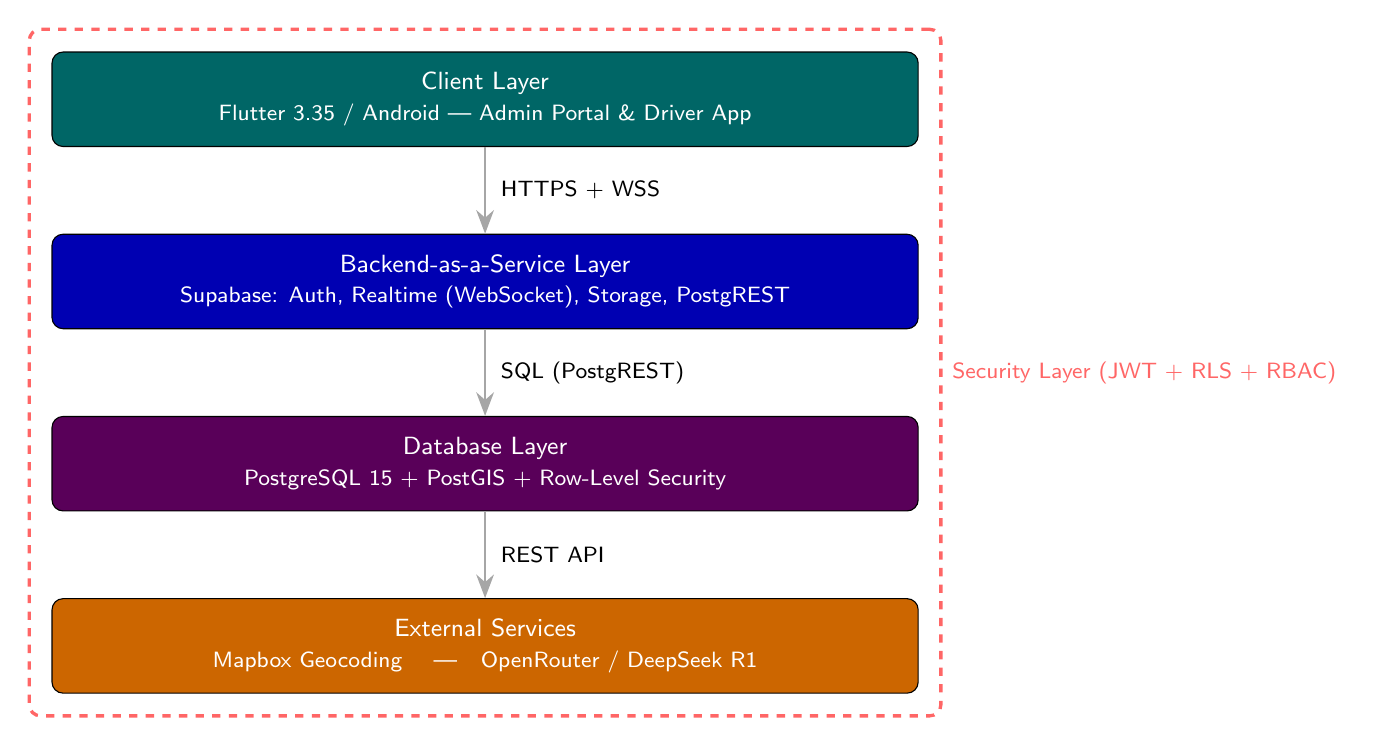
\begin{tikzpicture}[
    layer/.style={draw, rounded corners, minimum width=11cm, minimum height=1.2cm,
                  font=\sffamily\small, text=white, align=center},
    proto/.style={font=\sffamily\footnotesize, text=black},
    arr/.style={-{Stealth[length=3mm]}, thick, gray!70},
    node distance=1.1cm
  ]
    % Layers
    \node[layer, fill=teal!80!black]                       (client)   {Client Layer \\ \footnotesize Flutter 3.35 / Android — Admin Portal \& Driver App};
    \node[layer, fill=blue!70!black, below=of client]      (baas)     {Backend-as-a-Service Layer \\ \footnotesize Supabase: Auth, Realtime (WebSocket), Storage, PostgREST};
    \node[layer, fill=violet!70!black, below=of baas]      (db)       {Database Layer \\ \footnotesize PostgreSQL 15 + PostGIS + Row-Level Security};
    \node[layer, fill=orange!80!black, below=of db]        (ext)      {External Services \\ \footnotesize Mapbox Geocoding \quad|\quad OpenRouter / DeepSeek R1};

    % Security overlay
    \node[draw=red!60, dashed, very thick, rounded corners,
          fit=(client)(baas)(db)(ext),
          inner sep=8pt, label={[red!60, font=\sffamily\footnotesize]right:Security Layer (JWT + RLS + RBAC)}] {};

    % Protocol arrows
    \draw[arr] (client) -- node[proto, right, xshift=2pt] {HTTPS + WSS} (baas);
    \draw[arr] (baas)   -- node[proto, right, xshift=2pt] {SQL (PostgREST)} (db);
    \draw[arr] (db)     -- node[proto, right, xshift=2pt] {REST API} (ext);
  \end{tikzpicture}}%
  \caption{Four-layer architecture of OrderVista with cross-cutting security layer.}
  \label{fig:arch-layers}
\end{figure}

\paragraph{Alternatives considered.}
A traditional three-tier stack (e.g.\ Express.js + PostgreSQL + React Native)
was evaluated first.  Supabase was chosen instead because its hosted
PostgreSQL already includes Auth, Realtime, and Storage, eliminating the need
to write and deploy a custom API server.  This reduced the project scope to a
single-developer effort while preserving enterprise-grade security through
native RLS support \autocite{supabase2026docs}.  Firebase was rejected because
its document-oriented Firestore model lacks native RLS and makes relational
queries (e.g.\ joining routes to tasks to drivers) cumbersome
\autocite{abdul2018multitenant}.

\subsection{Deployment Architecture}
\label{sec:deployment}

Figure~\ref{fig:deployment} shows the physical deployment topology.  All
server-side components are managed services, eliminating operational overhead
for infrastructure provisioning.

\begin{figure}[ht]
  \centering
  \resizebox{0.94\textwidth}{!}{%
  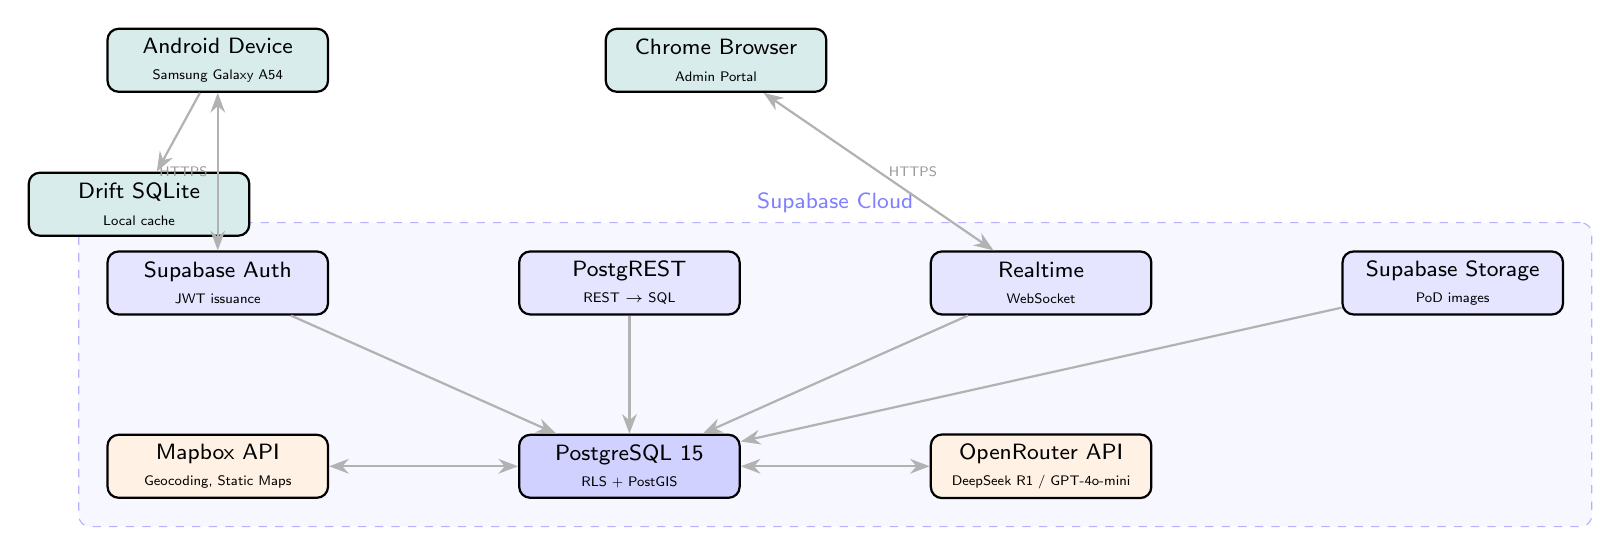
\begin{tikzpicture}[
    node/.style={draw, rounded corners=4pt, minimum width=2.8cm,
                 minimum height=0.8cm, font=\sffamily\footnotesize,
                 align=center, thick},
    device/.style={node, fill=teal!15},
    cloud/.style={node, fill=blue!10},
    ext/.style={node, fill=orange!10},
    arr/.style={-{Stealth[length=2.5mm]}, thick, gray!60},
    darr/.style={{Stealth[length=2.5mm]}-{Stealth[length=2.5mm]}, thick, gray!60},
    lbl/.style={font=\sffamily\tiny, text=gray!80},
    node distance=1.2cm and 2.4cm
  ]
    % Client devices
    \node[device]                            (android) {Android Device\\{\tiny Samsung Galaxy A54}};
    \node[device, right=3.5cm of android]    (web)     {Chrome Browser\\{\tiny Admin Portal}};

    % Supabase cloud
    \node[cloud, below=2cm of android]       (auth)    {Supabase Auth\\{\tiny JWT issuance}};
    \node[cloud, right=of auth]              (rest)    {PostgREST\\{\tiny REST $\to$ SQL}};
    \node[cloud, right=of rest]              (rt)      {Realtime\\{\tiny WebSocket}};
    \node[cloud, right=of rt]               (store)   {Supabase Storage\\{\tiny PoD images}};

    % Database
    \node[cloud, below=1.5cm of rest, fill=blue!18] (pg) {PostgreSQL 15\\{\tiny RLS + PostGIS}};

    % External
    \node[ext, left=of pg]                   (mapbox)  {Mapbox API\\{\tiny Geocoding, Static Maps}};
    \node[ext, right=of pg]                  (or)      {OpenRouter API\\{\tiny DeepSeek R1 / GPT-4o-mini}};

    % Local DB
    \node[device, below=1cm of android, xshift=-1cm]  (drift)  {Drift SQLite\\{\tiny Local cache}};

    % Grouping
    \begin{scope}[on background layer]
      \node[draw=blue!30, dashed, rounded corners, fill=blue!3,
            fit=(auth)(rest)(rt)(store)(pg),
            inner sep=10pt, label={[blue!50, font=\sffamily\footnotesize]above:Supabase Cloud}] {};
    \end{scope}

    % Connections
    \draw[darr] (android) -- node[lbl, left] {HTTPS} (auth);
    \draw[darr] (web) -- node[lbl, right] {HTTPS} (rt);
    \draw[arr]  (android) -- (drift);
    \draw[arr]  (auth) -- (pg);
    \draw[arr]  (rest) -- (pg);
    \draw[arr]  (rt) -- (pg);
    \draw[arr]  (store) -- (pg);
    \draw[darr] (pg) -- (mapbox);
    \draw[darr] (pg) -- (or);
  \end{tikzpicture}}%
  \caption{UML deployment diagram showing physical nodes and communication protocols.}
  \label{fig:deployment}
\end{figure}

% ─────────────────────────────────────────────────────────────
\section{Technology Stack}
\label{sec:tech-stack}

Table~\ref{tab:tech-stack} summarises the core technologies and the rationale
for each selection.

\begin{table}[ht]
  \centering
  \caption{Technology stack with alternatives considered.}
  \label{tab:tech-stack}
  \small
  \begin{tabularx}{\textwidth}{l l X}
    \toprule
    \textbf{Layer} & \textbf{Choice} & \textbf{Rationale / Alternatives} \\
    \midrule
    Mobile UI
      & Flutter 3.35
      & Single codebase for Android \& iOS; Skia renderer ensures pixel-perfect
        maps.  React Native was considered but its bridge-based architecture
        adds latency for map-heavy views
        \autocite{flutter2026docs}. \\
    Backend
      & Supabase (hosted)
      & Built-in Auth, Realtime, Storage, and PostgREST.  A custom Node.js API
        would require separate deployment and maintenance
        \autocite{supabase2026docs}. \\
    Database
      & PostgreSQL 15
      & Native RLS, PostGIS for spatial queries, JSONB for flexible telemetry
        payloads.  MySQL lacks RLS; MongoDB lacks relational joins
        \autocite{postgresql2026rls}. \\
    Geocoding
      & Mapbox Geocoding API
      & 100\,000 free requests/month; returns GeoJSON with structured address
        components.  Google Geocoding API was costlier for the same tier
        \autocite{mapbox2026geocoding}. \\
    AI / LLM
      & DeepSeek R1 / GPT-4o-mini via OpenRouter
      & Configurable model backend; DeepSeek~R1 provides chain-of-thought
        reasoning at \$0.14/M input tokens; GPT-4o-mini serves as a
        low-latency fallback.  Both accessed through OpenRouter's unified
        API gateway \autocite{deepseek2025r1,openrouter2026docs}. \\
    Local DB
      & Drift (SQLite)
      & Type-safe, reactive, compiles to native SQLite; enables offline-first
        with sync queue.  Hive lacks SQL expressiveness
        \autocite{drift2026docs}. \\
    Version Control
      & Git + GitHub
      & Branch-per-feature workflow; CI via GitHub Actions for APK builds. \\
    \bottomrule
  \end{tabularx}
\end{table}

% ─────────────────────────────────────────────────────────────
\section{Data Model}
\label{sec:data-model}

The PostgreSQL schema consists of thirteen tables distributed across three migrations.
Table~\ref{tab:schema} lists each table and its purpose; foreign-key
relationships are described in the text below.

\begin{table}[ht]
  \centering
  \caption{Database schema overview (13 tables).}
  \label{tab:schema}
  \small
  \begin{tabularx}{\textwidth}{l l X}
    \toprule
    \textbf{Table} & \textbf{PK Type} & \textbf{Purpose} \\
    \midrule
    \texttt{companies}          & UUID & Multi-tenant root; stores name and timezone. \\
    \texttt{company\_members}   & UUID & Maps \texttt{auth.users} to companies with a role
                                         (\texttt{driver}, \texttt{dispatcher}, \texttt{admin}). \\
    \texttt{vehicles}           & UUID & Fleet registry; links to an active route and assigned driver. \\
    \texttt{routes}             & UUID & Route header; references company, vehicle, driver; tracks
                                         status, optimizer type, and ETA summary (JSONB). \\
    \texttt{tasks}              & UUID & Individual delivery tasks with address, PostGIS
                                         \texttt{geography(point,4326)} location, priority, and
                                         proof-of-delivery fields. \\
    \texttt{route\_tasks}       & UUID & Join table; assigns a task to a route with a sequence
                                         number and planned arrival/departure. \\
    \texttt{telemetry\_events}  & BIGINT & GPS pings from drivers; includes speed, heading,
                                            battery, and a JSONB payload for extensibility. \\
    \texttt{sync\_queue\_items} & UUID & Offline-first write queue; stores pending mutations with
                                          retry count and backoff timestamp. \\
    \texttt{media\_artifacts}   & UUID & Photos and documents (PoD images); references Storage
                                          paths with optional checksums and expiry. \\
    \texttt{chat\_messages}     & UUID & Admin--driver messaging; supports directed and broadcast
                                          messages with read-receipt tracking. \\
    \texttt{notifications}      & UUID & System notifications for task assignments, status changes,
                                          and admin broadcasts. \\
    \texttt{geofence\_rules}    & UUID & Configurable geofence boundaries for delivery zones;
                                          supports future proximity-based alerts. \\
    \texttt{audit\_log}         & UUID & Immutable log of security-relevant events (logins, role
                                          changes, RLS denials) for compliance auditing. \\
    \bottomrule
  \end{tabularx}
\end{table}

\paragraph{Key relationships.}
Every table carries a \texttt{company\_id} foreign key, enforcing
tenant-scoped partitioning at the schema level.  \texttt{routes} reference
both a \texttt{vehicle} and a \texttt{driver} (both nullable for draft
routes).  \texttt{route\_tasks} forms the many-to-many join between routes
and tasks, with a unique compound constraint on
\texttt{(route\_id, sequence)} to guarantee ordering.  \texttt{tasks} stores
the PostGIS \texttt{geography} column used by the Haversine-based
nearest-neighbour sequencer at route-generation time.
Figure~\ref{fig:er} illustrates the principal foreign-key relationships.

\begin{figure}[ht]
  \centering
  \resizebox{0.92\textwidth}{!}{%
  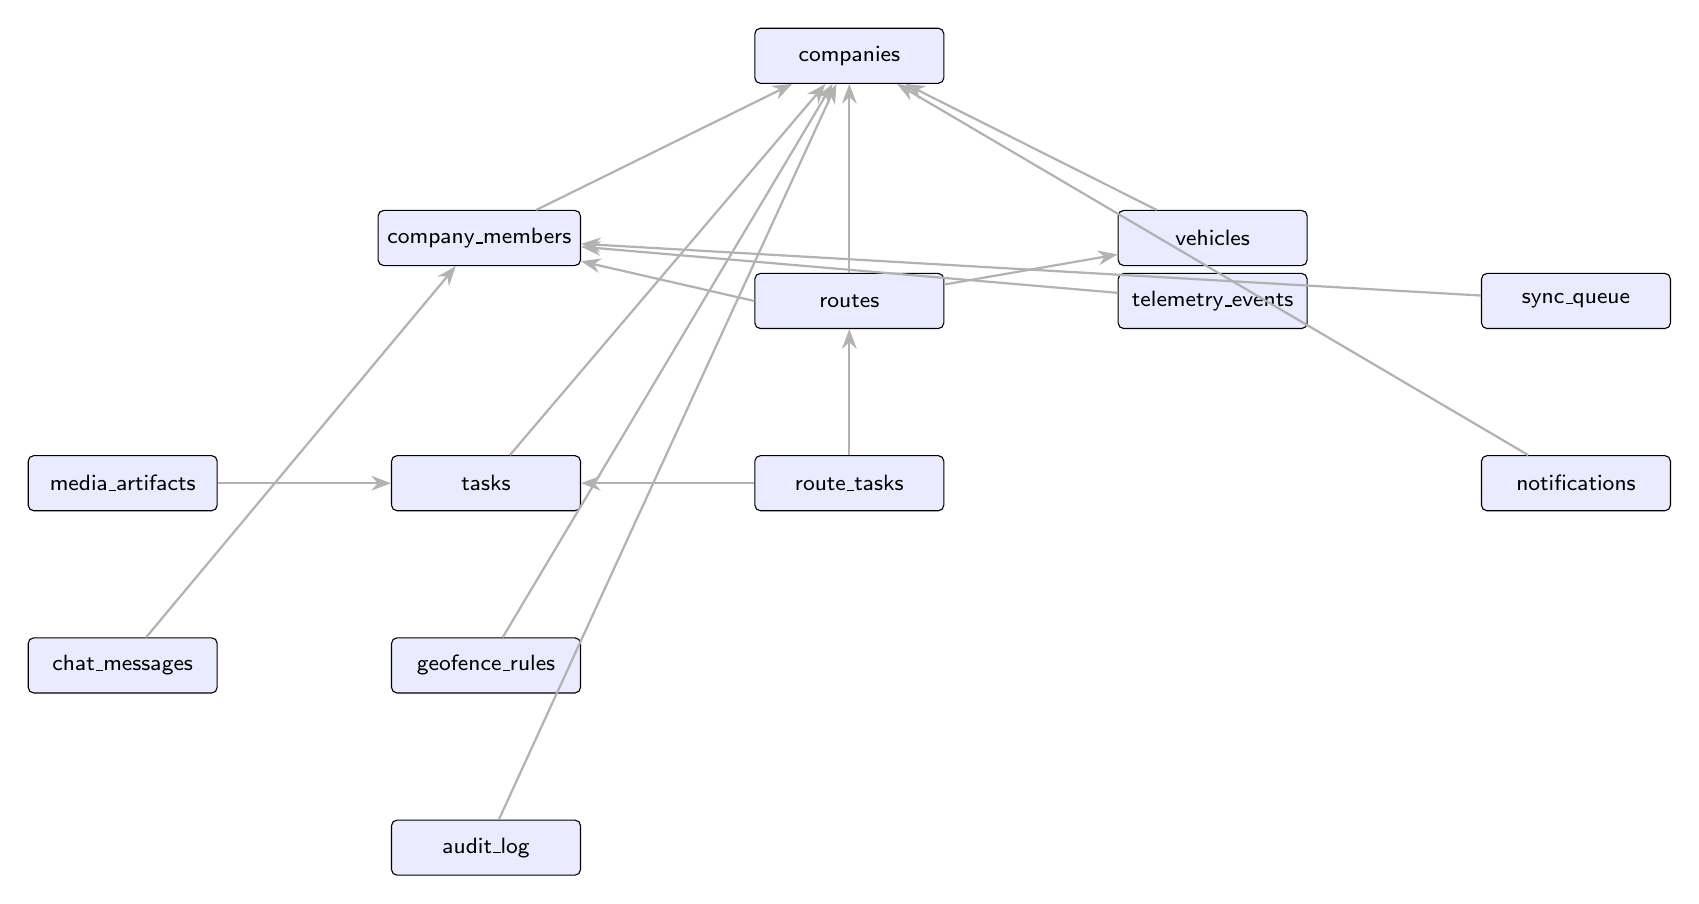
\begin{tikzpicture}[
    entity/.style={draw, rectangle, rounded corners=2pt,
                   minimum width=2.4cm, minimum height=0.7cm,
                   font=\sffamily\footnotesize, fill=blue!8},
    rel/.style={-{Stealth[length=2.5mm]}, thick, gray!60},
    node distance=1.6cm and 2.2cm
  ]
    % Core entities
    \node[entity]                            (comp)  {companies};
    \node[entity, below left=of comp]        (mem)   {company\_members};
    \node[entity, below right=of comp]       (veh)   {vehicles};
    \node[entity, below=2.4cm of comp]       (route) {routes};
    \node[entity, below left=of route]       (task)  {tasks};
    \node[entity, below=of route]            (rtask) {route\_tasks};
    \node[entity, right=of route]            (telem) {telemetry\_events};
    \node[entity, left=of task]              (media) {media\_artifacts};
    \node[entity, right=of telem]            (sync)  {sync\_queue};
    \node[entity, below=of media]            (chat)  {chat\_messages};
    \node[entity, below=of sync]             (notif) {notifications};
    \node[entity, below right=of chat]       (audit) {audit\_log};
    \node[entity, below=of task]             (geo)   {geofence\_rules};

    % Foreign keys
    \draw[rel] (mem)   -- (comp);
    \draw[rel] (veh)   -- (comp);
    \draw[rel] (route) -- (comp);
    \draw[rel] (route) -- (veh);
    \draw[rel] (route.west) -- (mem);
    \draw[rel] (task)  -- (comp);
    \draw[rel] (rtask) -- (route);
    \draw[rel] (rtask) -- (task);
    \draw[rel] (telem) -- (mem);
    \draw[rel] (media) -- (task);
    \draw[rel] (sync)  -- (mem);
    \draw[rel] (chat)  -- (mem);
    \draw[rel] (notif) -- (comp);
    \draw[rel] (audit) -- (comp);
    \draw[rel] (geo)   -- (comp);
  \end{tikzpicture}}%
  \caption{Entity-relationship overview — arrows denote foreign-key references.}
  \label{fig:er}
\end{figure}

\paragraph{Alternatives considered.}
A NoSQL document model (e.g.\ Firestore collections) would have simplified
schema evolution but would have required application-level joins and forfeited
PostGIS spatial indexing.  The relational model was preferred because the core
domain—routes comprising ordered tasks assigned to drivers—is inherently
relational, and PostGIS enables efficient distance calculations directly in
SQL \autocite{postgresql2026rls}.

% ─────────────────────────────────────────────────────────────
\section{Security Design}
\label{sec:security}

Security in OrderVista is enforced at three complementary levels:
authentication, row-level security, and role-based access control.

\subsection{Authentication}
\label{sec:authn}

Supabase Auth issues JWTs upon email/password login.  Every subsequent
PostgREST and Realtime request carries the JWT, which PostgreSQL validates
internally via the \texttt{auth.uid()} function.  This removes the need for
a custom authentication middleware \autocite{supabase2026docs}.

\subsection{Row-Level Security (RLS)}
\label{sec:rls}

Eleven of the thirteen tables have RLS enabled; \texttt{audit\_log}
(immutable, insert-only) and \texttt{geofence\_rules} (reserved for future
use) are exempt.  A shared helper function,
\texttt{is\_company\_member(company\_id)}, returns \texttt{true} only when the
authenticated user belongs to the specified company.  Every \texttt{SELECT},
\texttt{INSERT}, \texttt{UPDATE}, and \texttt{DELETE} policy on the eleven
RLS-protected tables invokes this function, guaranteeing that a query can
never read or modify rows belonging to a different tenant
\autocite{postgresql2026rls,aws2020rls}.

For chat messages, additional fine-grained policies restrict reads to the
sender, recipient, or broadcast scope, and restrict \texttt{UPDATE} (marking
messages as read) to the designated recipient.

\subsection{Role-Based Access Control (RBAC)}
\label{sec:rbac}

Table~\ref{tab:rbac} summarises the permission matrix.

\begin{table}[ht]
  \centering
  \caption{RBAC permission matrix (admin vs.\ driver).}
  \label{tab:rbac}
  \small
  \begin{tabularx}{\textwidth}{X c c}
    \toprule
    \textbf{Capability} & \textbf{Admin} & \textbf{Driver} \\
    \midrule
    Create / edit / delete tasks            & \checkmark & --- \\
    Import tasks via CSV                    & \checkmark & --- \\
    Generate and assign routes              & \checkmark & --- \\
    View all drivers and their locations    & \checkmark & --- \\
    Review proof-of-delivery submissions    & \checkmark & --- \\
    View assigned task list                 & \checkmark & \checkmark \\
    Update task status (in-progress, done)  & --- & \checkmark \\
    Capture PoD photo and signature         & --- & \checkmark \\
    Use AI assistant (summary \& chat)      & \checkmark & \checkmark \\
    Send / receive chat messages            & \checkmark & \checkmark \\
    \bottomrule
  \end{tabularx}
\end{table}

\paragraph{Alternatives considered.}
Application-level authorisation (e.g.\ middleware guards) was considered but
rejected because it cannot protect against direct database access or
misconfigured API endpoints.  Database-level RLS ensures that even if the API
layer is bypassed, data isolation is maintained—a well-established pattern
for multi-tenant SaaS systems \autocite{gao2011nonintrusive}.

\subsection{Task Lifecycle}
\label{sec:task-lifecycle}

Each delivery task follows a three-state lifecycle enforced by both the UI
and the database layer.  Figure~\ref{fig:task-fsm} visualises the permitted
transitions together with the actor responsible for each.

\begin{figure}[ht]
  \centering
  \resizebox{0.88\textwidth}{!}{%
  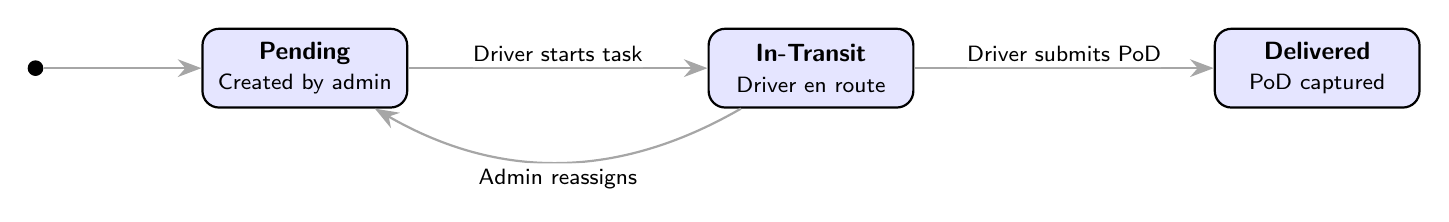
\begin{tikzpicture}[
    state/.style={draw, rounded corners=6pt, minimum width=2.6cm,
                  minimum height=1cm, font=\sffamily\small,
                  fill=blue!10, align=center, thick},
    init/.style={circle, fill=black, inner sep=2pt},
    arr/.style={-{Stealth[length=3mm]}, thick, gray!70},
    lbl/.style={font=\sffamily\footnotesize, text=black, fill=white,
                inner sep=2pt, rounded corners=2pt},
    node distance=3.8cm
  ]
    % States
    \node[init]                      (dot)       {};
    \node[state, right=2cm of dot]   (pending)   {\textbf{Pending}\\{\footnotesize Created by admin}};
    \node[state, right=of pending]   (transit)   {\textbf{In-Transit}\\{\footnotesize Driver en route}};
    \node[state, right=of transit]   (delivered) {\textbf{Delivered}\\{\footnotesize PoD captured}};

    % Transitions
    \draw[arr] (dot)       -- (pending);
    \draw[arr] (pending)   -- node[lbl, above] {Driver starts task} (transit);
    \draw[arr] (transit)   -- node[lbl, above] {Driver submits PoD} (delivered);

    % Re-assignment loop
    \draw[arr] (transit) to[out=-150,in=-30]
      node[lbl, below] {Admin reassigns} (pending);
  \end{tikzpicture}}%
  \caption{Task lifecycle state machine with permitted transitions.}
  \label{fig:task-fsm}
\end{figure}

% ─────────────────────────────────────────────────────────────
\section{External Service Integration}
\label{sec:external}

\subsection{Mapbox Geocoding and Static Maps}
\label{sec:mapbox}

When an admin creates a task, the address string is sent to the Mapbox
Geocoding API, which returns latitude/longitude coordinates stored as a
PostGIS \texttt{geography} point.  The geocoded location is subsequently
used by the nearest-neighbour route sequencer and by the static-map tile
generator, which renders a preview image of the planned route for the admin
dashboard \autocite{mapbox2026geocoding}.

\subsection{DeepSeek~R1 via OpenRouter}
\label{sec:deepseek}

The AI assistant calls DeepSeek~R1 through the OpenRouter proxy, which
provides a single API key and unified billing across multiple LLM providers.
Two prompt templates are employed:

\begin{itemize}
  \item \textbf{Summary prompt} — injects the current driver's task list,
        route status, and fleet statistics into a system prompt, requesting a
        concise natural-language summary.
  \item \textbf{Chat prompt} — extends the summary context with the user's
        free-text question and a JSON action schema, enabling the model to
        return structured actions (e.g.\ \texttt{\{"action": "re\_sequence",
        "params": \{"route\_id": "..."\}\}}) that the client can execute with
        a single confirmation tap.
\end{itemize}

This agentic pattern—where the LLM proposes actions and the user confirms—was
chosen over full autonomous execution to prevent hallucination-induced errors,
a known LLM reliability concern \autocite{ji2024hallucination}.

% ─────────────────────────────────────────────────────────────
\section{Critical System Flows}
\label{sec:flows}

\subsection{Administrative Workflow}
\label{sec:admin-flow}

The admin follows an eight-step workflow:

\begin{enumerate}
  \item \textbf{Task creation} — manual entry or bulk CSV import with
        validation (required fields: address, optional: time window, priority,
        notes).
  \item \textbf{Geocoding} — each task address is geocoded via Mapbox; failures
        are flagged for manual correction.
  \item \textbf{Route generation} — the nearest-neighbour heuristic sequences
        tasks by Haversine distance from a configurable depot.
  \item \textbf{Driver recommendation} — a composite score combining task
        proximity, current workload, historical on-time rate, and average
        completion time ranks available drivers.
  \item \textbf{Route assignment} — the admin reviews the recommended driver,
        map preview, and estimated distances, then confirms assignment.
  \item \textbf{Monitoring} — real-time Supabase subscriptions push driver
        location, task status changes, and telemetry events to the admin
        dashboard.
  \item \textbf{Mid-shift intervention} — if conditions change, the admin (or
        AI assistant) can trigger re-sequencing from the driver's current GPS
        position.
  \item \textbf{PoD review} — upon delivery completion, the admin reviews the
        uploaded photo, signature, and confirmation code.
\end{enumerate}

\subsection{Driver Workflow}
\label{sec:driver-flow}

\begin{enumerate}
  \item \textbf{Authentication} — email/password login; JWT issued.
  \item \textbf{Task list} — assigned tasks displayed in sequence order with
        real-time status badges.
  \item \textbf{Navigation} — tapping a task opens the address in the device's
        default maps application.
  \item \textbf{Status progression} — the driver marks each task as
        \emph{in-progress} and then \emph{completed}.
  \item \textbf{PoD capture} — mandatory photo and optional signature before
        a task can be marked complete.
  \item \textbf{Sync} — completed tasks are written to the local Drift
        database and enqueued for upload; the sync queue retries with
        exponential backoff if connectivity is lost.
  \item \textbf{AI assistant} — the driver can request a summary of remaining
        work or ask free-form questions about their route.
\end{enumerate}

\subsection{Offline Synchronisation}
\label{sec:offline-sync}

OrderVista follows an offline-first pattern.  All writes are persisted to the
local Drift (SQLite) database before being enqueued in the
\texttt{sync\_queue\_items} table.  A background isolate processes the queue
with a progressive backoff schedule (0, 10, 30, 60, 120\,s delays, up to five
attempts).  On reconnection, Supabase
Realtime subscriptions automatically push any server-side changes that
occurred while the device was offline, and the client reconciles state via
\texttt{updated\_at} timestamps.  Offline-first design is widely recommended
for mobile applications that must remain usable under unreliable network
conditions; modern frameworks commonly employ local caching and deferred
synchronisation to provide an ``always-on'' user experience
\autocite{gaur2024offlinefirst}.  This design ensures that drivers operating
in areas with intermittent cellular coverage, which is common in Hong Kong's
industrial estates, can continue capturing deliveries without data loss.

% ─────────────────────────────────────────────────────────────
\section{Interaction Sequences}
\label{sec:sequences}

This section formalises the two most architecturally significant interactions
as UML-style sequence diagrams: task creation with route generation
(Figure~\ref{fig:seq-task}) and the agentic AI suggestion cycle
(Figure~\ref{fig:seq-agentic}).

\subsection{Task Creation and Route Assignment}
\label{sec:seq-task}

Figure~\ref{fig:seq-task} traces the complete lifecycle of a task batch from
CSV import through route generation to driver notification.

\begin{figure}[ht]
  \centering
  \resizebox{\textwidth}{!}{%
  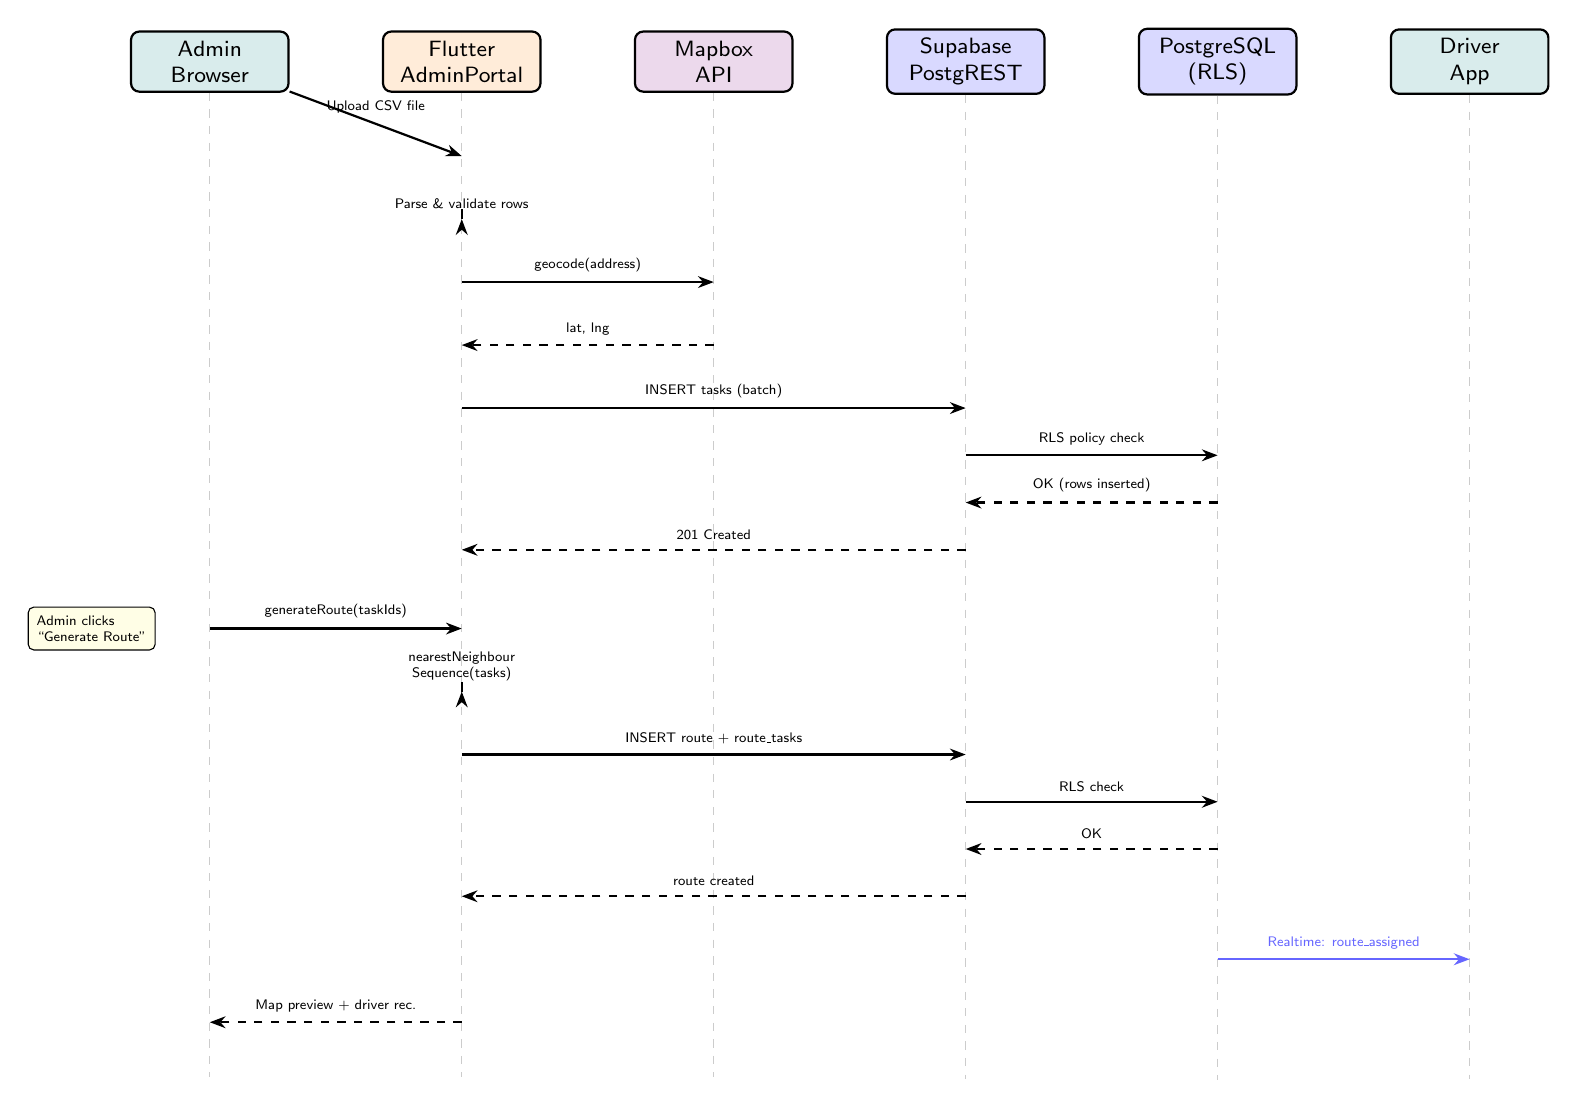
\begin{tikzpicture}[
    actor/.style={draw, rectangle, rounded corners=3pt, minimum width=2cm,
                  minimum height=0.7cm, font=\sffamily\footnotesize,
                  fill=#1!15, align=center, thick},
    msg/.style={-{Stealth[length=2mm]}, thick, font=\sffamily\tiny},
    ret/.style={-{Stealth[length=2mm]}, thick, dashed, font=\sffamily\tiny},
    note/.style={draw, rectangle, rounded corners=2pt, fill=yellow!10,
                 font=\sffamily\tiny, align=left, inner sep=3pt},
  ]
    % Participants
    \node[actor=teal]   (admin)  at (0,0)    {Admin\\Browser};
    \node[actor=orange]  (flutter) at (3.2,0)  {Flutter\\AdminPortal};
    \node[actor=violet]  (mapbox)  at (6.4,0)  {Mapbox\\API};
    \node[actor=blue]   (supa)   at (9.6,0)  {Supabase\\PostgREST};
    \node[actor=blue]   (pg)     at (12.8,0) {PostgreSQL\\(RLS)};
    \node[actor=teal]   (driver) at (16,0)   {Driver\\App};

    % Lifelines
    \foreach \n in {admin, flutter, mapbox, supa, pg, driver} {
      \draw[dashed, gray!40] (\n.south) -- ++(0,-12.5);
    }

    % Messages
    \def\y{-1.2}
    \draw[msg] (admin) -- node[above] {Upload CSV file} (flutter |- 0,\y);
    \def\y{-2.0}
    \draw[msg] (flutter |- 0,\y) -- node[above] {Parse \& validate rows} (flutter |- 0,\y);
    \def\y{-2.8}
    \draw[msg] (flutter |- 0,\y) -- node[above] {geocode(address)} (mapbox |- 0,\y);
    \def\y{-3.6}
    \draw[ret] (mapbox |- 0,\y) -- node[above] {lat, lng} (flutter |- 0,\y);
    \def\y{-4.4}
    \draw[msg] (flutter |- 0,\y) -- node[above] {INSERT tasks (batch)} (supa |- 0,\y);
    \def\y{-5.0}
    \draw[msg] (supa |- 0,\y) -- node[above] {RLS policy check} (pg |- 0,\y);
    \def\y{-5.6}
    \draw[ret] (pg |- 0,\y) -- node[above] {OK (rows inserted)} (supa |- 0,\y);
    \def\y{-6.2}
    \draw[ret] (supa |- 0,\y) -- node[above] {201 Created} (flutter |- 0,\y);

    % Route generation
    \def\y{-7.2}
    \node[note] at (-1.5, \y) {Admin clicks\\``Generate Route''};
    \draw[msg] (admin |- 0,\y) -- node[above] {generateRoute(taskIds)} (flutter |- 0,\y);
    \def\y{-8.0}
    \draw[msg] (flutter |- 0,\y) -- node[above, align=center] {nearestNeighbour\\Sequence(tasks)} (flutter |- 0,\y);
    \def\y{-8.8}
    \draw[msg] (flutter |- 0,\y) -- node[above] {INSERT route + route\_tasks} (supa |- 0,\y);
    \def\y{-9.4}
    \draw[msg] (supa |- 0,\y) -- node[above] {RLS check} (pg |- 0,\y);
    \def\y{-10.0}
    \draw[ret] (pg |- 0,\y) -- node[above] {OK} (supa |- 0,\y);
    \def\y{-10.6}
    \draw[ret] (supa |- 0,\y) -- node[above] {route created} (flutter |- 0,\y);

    % Realtime notification
    \def\y{-11.4}
    \draw[msg, blue!60] (pg |- 0,\y) -- node[above, blue!60] {Realtime: route\_assigned} (driver |- 0,\y);
    \def\y{-12.2}
    \draw[ret] (flutter |- 0,\y) -- node[above] {Map preview + driver rec.} (admin |- 0,\y);
  \end{tikzpicture}}%
  \caption{Sequence diagram: task creation via CSV import, geocoding,
           route generation, and real-time driver notification.}
  \label{fig:seq-task}
\end{figure}

\subsection{Agentic AI Suggestion Cycle}
\label{sec:seq-agentic}

Figure~\ref{fig:seq-agentic} details the interaction between the driver
application, the AI service, and the remote LLM when producing an agentic
suggestion with a one-tap executable action.

\begin{figure}[ht]
  \centering
  \resizebox{0.92\textwidth}{!}{%
  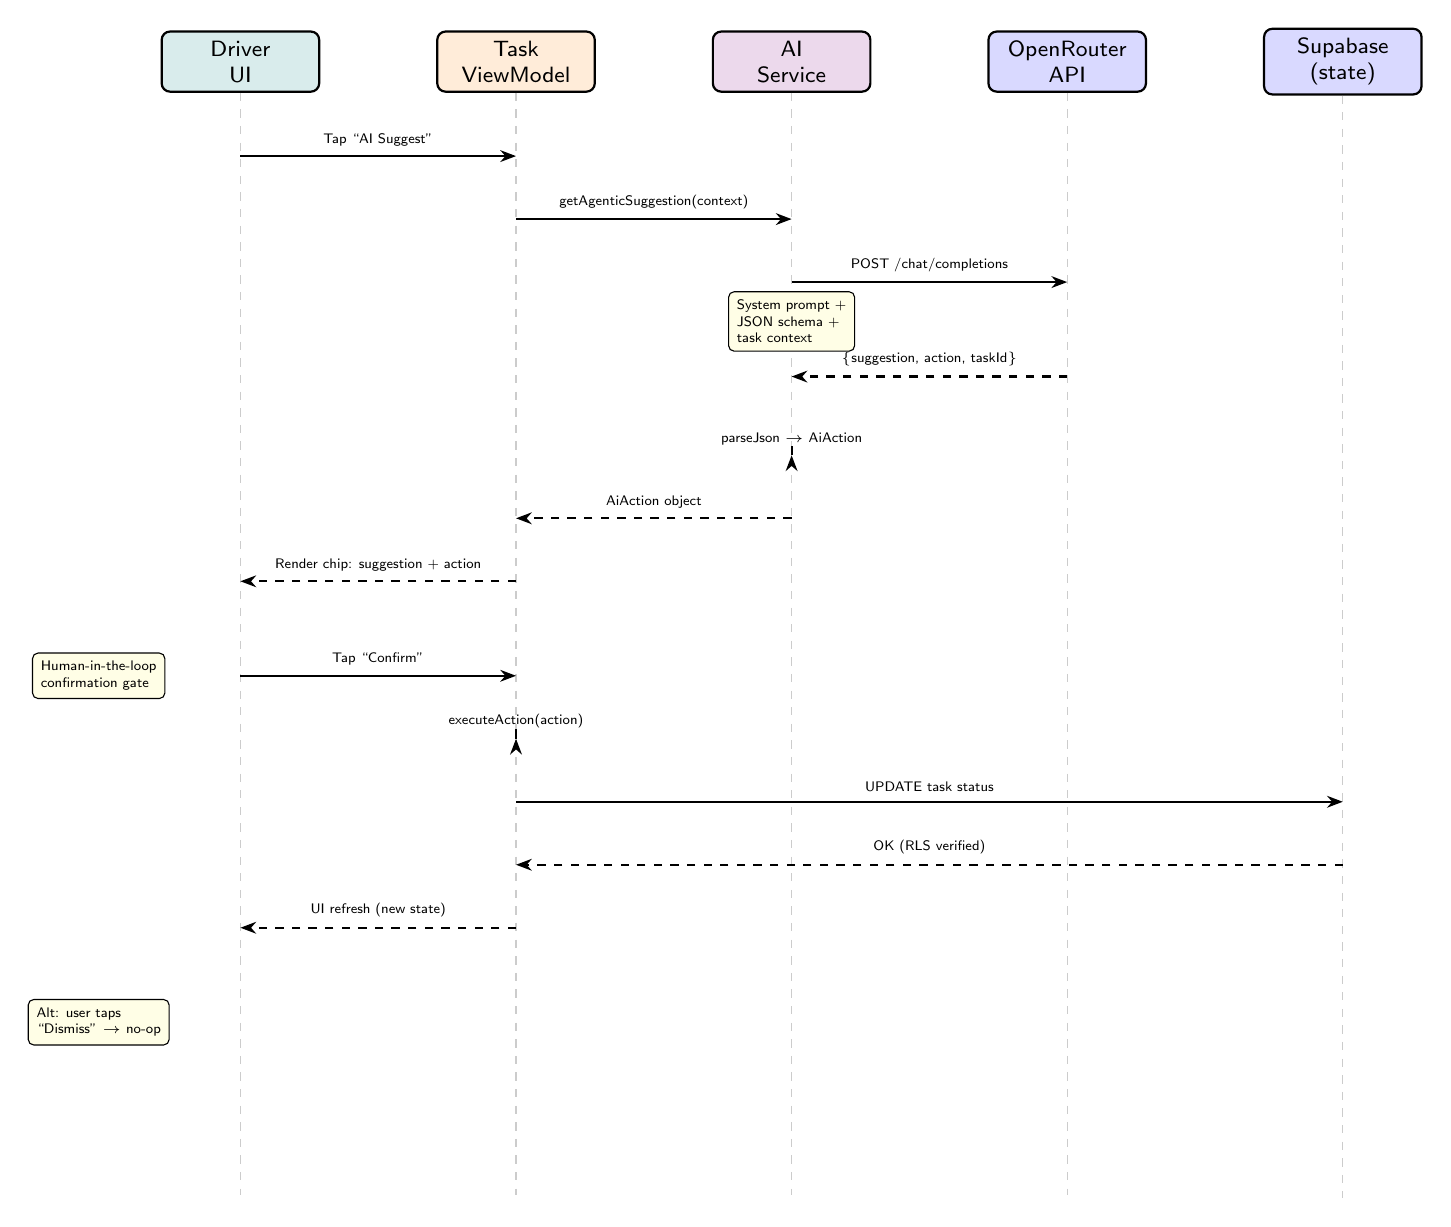
\begin{tikzpicture}[
    actor/.style={draw, rectangle, rounded corners=3pt, minimum width=2cm,
                  minimum height=0.7cm, font=\sffamily\footnotesize,
                  fill=#1!15, align=center, thick},
    msg/.style={-{Stealth[length=2mm]}, thick, font=\sffamily\tiny},
    ret/.style={-{Stealth[length=2mm]}, thick, dashed, font=\sffamily\tiny},
    note/.style={draw, rectangle, rounded corners=2pt, fill=yellow!10,
                 font=\sffamily\tiny, align=left, inner sep=3pt},
    alt/.style={draw, dashed, rounded corners=2pt, fill=green!5, inner sep=4pt},
  ]
    % Participants
    \node[actor=teal]   (driver)  at (0,0)    {Driver\\UI};
    \node[actor=orange]  (taskvm)  at (3.5,0)  {Task\\ViewModel};
    \node[actor=violet]  (aisvc)   at (7,0)    {AI\\Service};
    \node[actor=blue]   (openr)   at (10.5,0) {OpenRouter\\API};
    \node[actor=blue]   (supa)    at (14,0)   {Supabase\\(state)};

    % Lifelines
    \foreach \n in {driver, taskvm, aisvc, openr, supa} {
      \draw[dashed, gray!40] (\n.south) -- ++(0,-14);
    }

    % Messages
    \def\y{-1.2}
    \draw[msg] (driver |- 0,\y) -- node[above] {Tap ``AI Suggest''} (taskvm |- 0,\y);
    \def\y{-2.0}
    \draw[msg] (taskvm |- 0,\y) -- node[above] {getAgenticSuggestion(context)} (aisvc |- 0,\y);
    \def\y{-2.8}
    \node[note] at (7, -3.3) {System prompt +\\JSON schema +\\task context};
    \draw[msg] (aisvc |- 0,\y) -- node[above] {POST /chat/completions} (openr |- 0,\y);
    \def\y{-4.0}
    \draw[ret] (openr |- 0,\y) -- node[above] {\{suggestion, action, taskId\}} (aisvc |- 0,\y);

    % Parse
    \def\y{-5.0}
    \draw[msg] (aisvc |- 0,\y) -- node[above] {parseJson $\to$ AiAction} (aisvc |- 0,\y);
    \def\y{-5.8}
    \draw[ret] (aisvc |- 0,\y) -- node[above] {AiAction object} (taskvm |- 0,\y);
    \def\y{-6.6}
    \draw[ret] (taskvm |- 0,\y) -- node[above] {Render chip: suggestion + action} (driver |- 0,\y);

    % User decision
    \def\y{-7.8}
    \node[note] at (-1.8, \y) {Human-in-the-loop\\confirmation gate};
    \draw[msg] (driver |- 0,\y) -- node[above] {Tap ``Confirm''} (taskvm |- 0,\y);
    \def\y{-8.6}
    \draw[msg] (taskvm |- 0,\y) -- node[above] {executeAction(action)} (taskvm |- 0,\y);

    % State update
    \def\y{-9.4}
    \draw[msg] (taskvm |- 0,\y) -- node[above] {UPDATE task status} (supa |- 0,\y);
    \def\y{-10.2}
    \draw[ret] (supa |- 0,\y) -- node[above] {OK (RLS verified)} (taskvm |- 0,\y);
    \def\y{-11.0}
    \draw[ret] (taskvm |- 0,\y) -- node[above] {UI refresh (new state)} (driver |- 0,\y);

    % Alt: reject
    \def\y{-12.2}
    \node[note] at (-1.8, \y) {Alt: user taps\\``Dismiss'' $\to$ no-op};
  \end{tikzpicture}}%
  \caption{Sequence diagram: agentic AI suggestion with human-in-the-loop
           confirmation and state synchronisation.}
  \label{fig:seq-agentic}
\end{figure}

The key design insight is the \emph{confirmation gate} between steps~6 and~7:
the LLM's suggestion is never executed automatically.  This addresses the
inherent unreliability of LLM outputs in safety-critical logistics operations
\autocite{ji2024hallucination} and distinguishes OrderVista's agentic approach
from fully autonomous AI agents.

% Chapter 4: Implementation
\chapter{Implementation}
\label{ch:implementation}

This chapter describes the development methodology and the key implementation
details of OrderVista, including algorithmic components, the AI integration
layer, and the offline synchronisation mechanism.

% ─────────────────────────────────────────────────────────────
\section{Development Methodology}
\label{sec:methodology}

An iterative, incremental approach was adopted over five phases spanning six
months (October 2025 to March 2026):

\begin{enumerate}
  \item \textbf{Foundation} (Oct) — project scaffolding, Supabase schema
        migration, authentication flow, basic CRUD screens.
  \item \textbf{Core Implementation} (Nov) — admin task management, CSV import
        with validation, driver task list with real-time subscriptions.
  \item \textbf{Feature Development} (Dec--Jan) — route generation with
        geocoding, proof-of-delivery workflow, AI summarisation and chat.
  \item \textbf{Integration} (Feb) — agentic AI actions, driver
        recommendation, fleet-wide optimisation, chat messaging.
  \item \textbf{Refinement} (Mar) — dynamic priority, mid-shift
        re-sequencing, performance metrics, security hardening, release build.
\end{enumerate}

Each phase concluded with a working APK build and a supervisor progress
review, ensuring that feedback could be incorporated before the next phase.
Version control followed a branch-per-feature model on GitHub with a single
integration branch (\texttt{feature/\allowbreak delivery-optimization-mvp}).

Figure~\ref{fig:mvvm} illustrates the layered MVVM architecture used
throughout the codebase.  Each layer communicates only with its immediate
neighbour, enforcing separation of concerns and testability.

\begin{figure}[ht]
  \centering
  \resizebox{0.82\textwidth}{!}{%
  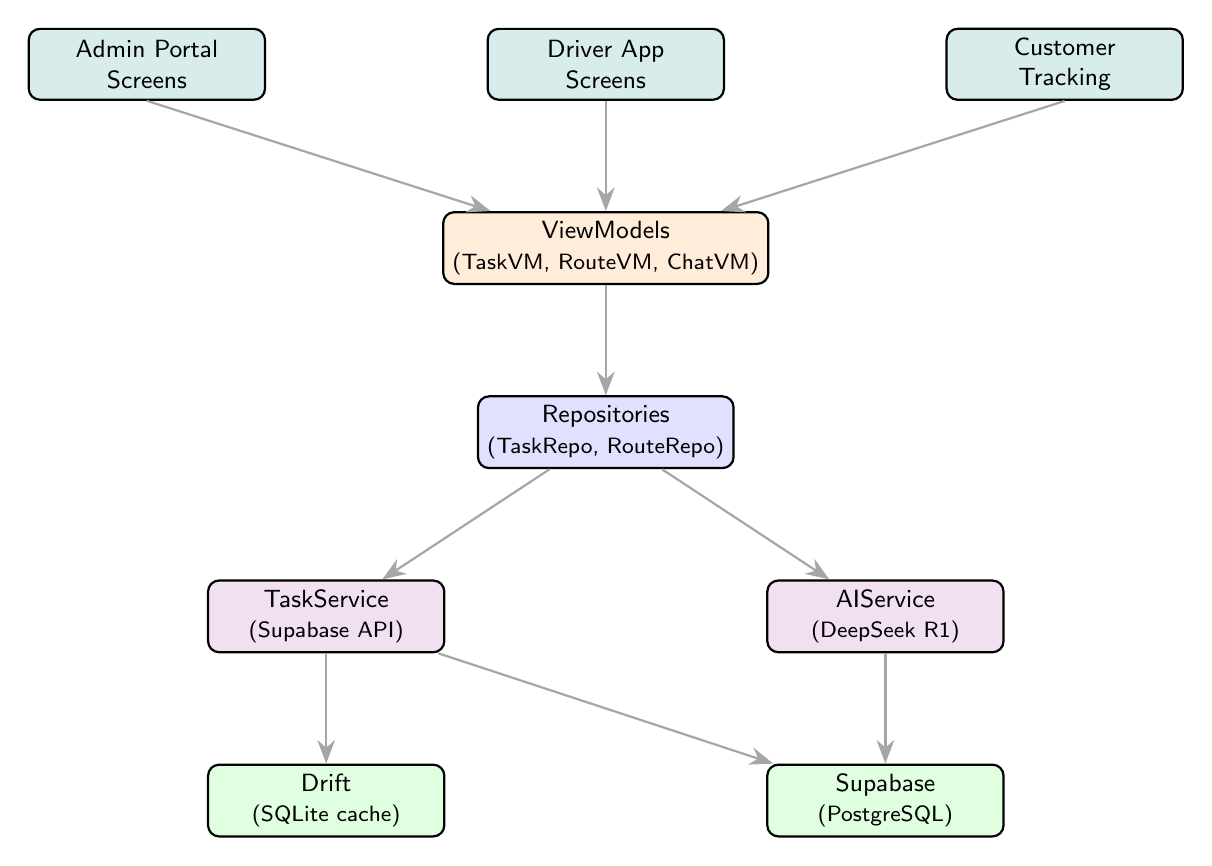
\begin{tikzpicture}[
    box/.style={draw, rounded corners=4pt, minimum width=3cm,
                minimum height=0.9cm, font=\sffamily\small,
                align=center, thick},
    arr/.style={-{Stealth[length=3mm]}, thick, gray!70},
    node distance=1.4cm and 2.8cm
  ]
    % View layer
    \node[box, fill=teal!15]                     (v1) {Admin Portal\\Screens};
    \node[box, fill=teal!15, right=of v1]        (v2) {Driver App\\Screens};
    \node[box, fill=teal!15, right=of v2]        (v3) {Customer\\Tracking};

    % ViewModel layer
    \node[box, fill=orange!15, below=of v2]      (vm) {ViewModels\\{\footnotesize(TaskVM, RouteVM, ChatVM)}};

    % Repository layer
    \node[box, fill=blue!12, below=of vm]        (repo) {Repositories\\{\footnotesize(TaskRepo, RouteRepo)}};

    % Service layer
    \node[box, fill=violet!12, below left=1.4cm and 0.4cm of repo]  (svc1) {TaskService\\{\footnotesize(Supabase API)}};
    \node[box, fill=violet!12, below right=1.4cm and 0.4cm of repo] (svc2) {AIService\\{\footnotesize(DeepSeek R1)}};

    % Data layer
    \node[box, fill=green!12, below=1.4cm of svc1]  (drift) {Drift\\{\footnotesize(SQLite cache)}};
    \node[box, fill=green!12, below=1.4cm of svc2]  (supa)  {Supabase\\{\footnotesize(PostgreSQL)}};

    % Arrows
    \draw[arr] (v1.south) -- (vm);
    \draw[arr] (v2)       -- (vm);
    \draw[arr] (v3.south) -- (vm);
    \draw[arr] (vm)       -- (repo);
    \draw[arr] (repo)     -- (svc1);
    \draw[arr] (repo)     -- (svc2);
    \draw[arr] (svc1)     -- (drift);
    \draw[arr] (svc1)     -- (supa);
    \draw[arr] (svc2)     -- (supa);
  \end{tikzpicture}}%
  \caption{MVVM layered architecture: Views $\to$ ViewModels $\to$ Repositories $\to$ Services $\to$ Data.}
  \label{fig:mvvm}
\end{figure}

Figure~\ref{fig:class-diagram} expands the MVVM layers into a UML class
diagram showing the principal classes, their attributes, and
inter-class dependencies.

\begin{figure}[ht]
  \centering
  \resizebox{\textwidth}{!}{%
  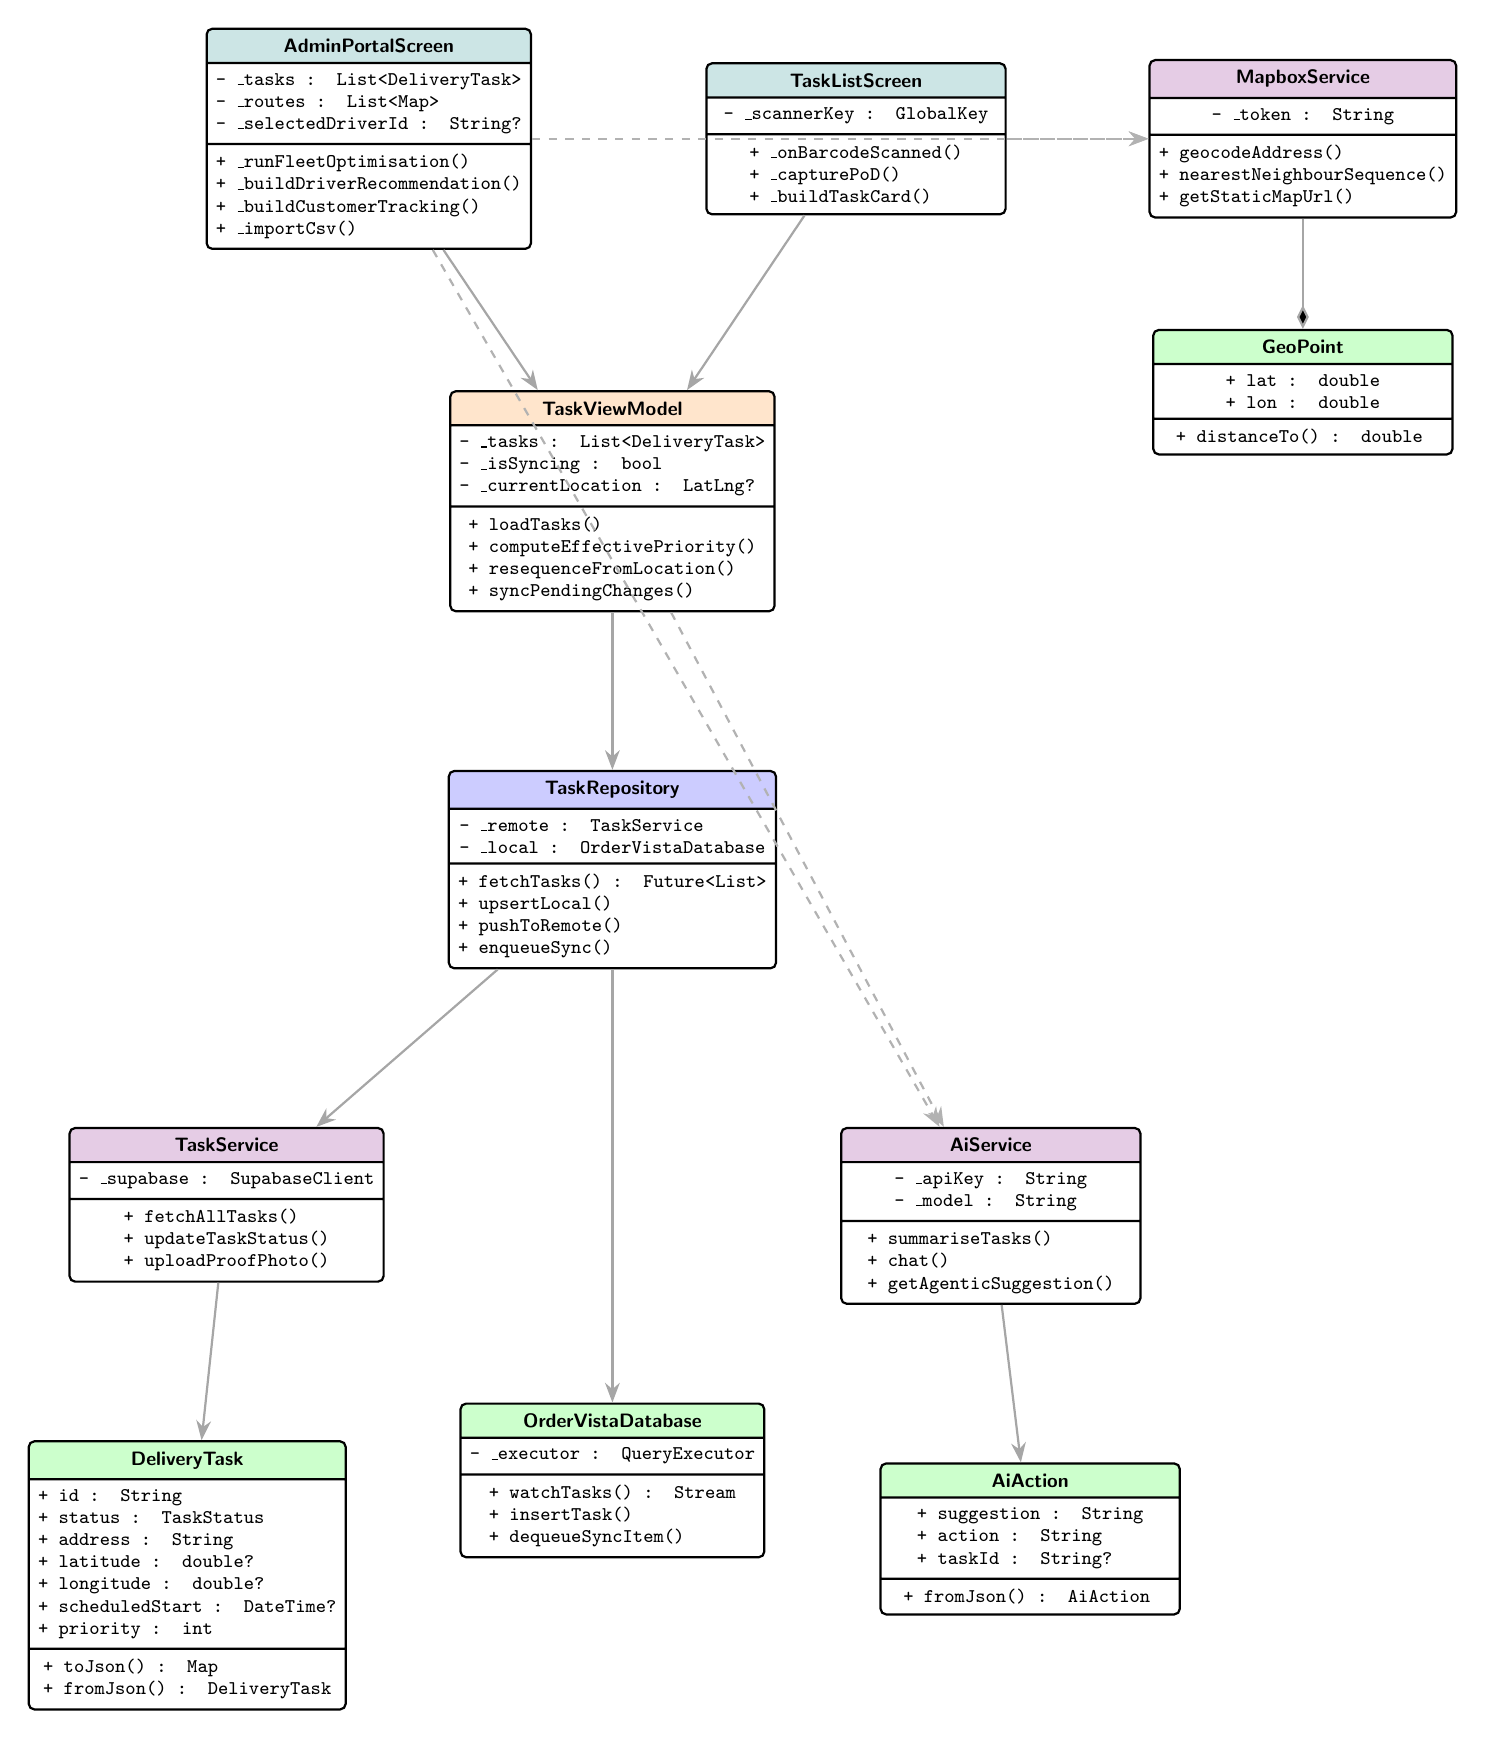
\begin{tikzpicture}[
    class/.style={draw, rectangle split, rectangle split parts=3,
                  rectangle split part fill={#1!20, white, white},
                  rounded corners=2pt, font=\sffamily\scriptsize,
                  minimum width=3.8cm, thick, align=left},
    arr/.style={-{Stealth[length=2.5mm]}, thick, gray!70},
    comp/.style={-{Diamond[length=3mm, fill=black]}, thick, gray!70},
    uses/.style={-{Stealth[length=2.5mm]}, thick, dashed, gray!60},
    node distance=1.6cm and 1.4cm
  ]
    %% ── View layer ──────────────────────────────────
    \node[class=teal] (admin) {
      \textbf{AdminPortalScreen}
      \nodepart{second}
      \texttt{- \_tasks : List<DeliveryTask>}\\
      \texttt{- \_routes : List<Map>}\\
      \texttt{- \_selectedDriverId : String?}
      \nodepart{third}
      \texttt{+ \_runFleetOptimisation()}\\
      \texttt{+ \_buildDriverRecommendation()}\\
      \texttt{+ \_buildCustomerTracking()}\\
      \texttt{+ \_importCsv()}
    };

    \node[class=teal, right=2.2cm of admin] (tasklist) {
      \textbf{TaskListScreen}
      \nodepart{second}
      \texttt{- \_scannerKey : GlobalKey}
      \nodepart{third}
      \texttt{+ \_onBarcodeScanned()}\\
      \texttt{+ \_capturePoD()}\\
      \texttt{+ \_buildTaskCard()}
    };

    %% ── ViewModel layer ─────────────────────────────
    \node[class=orange, below=2cm of $(admin.south)!0.5!(tasklist.south)$] (taskvm) {
      \textbf{TaskViewModel}
      \nodepart{second}
      \texttt{- \_tasks : List<DeliveryTask>}\\
      \texttt{- \_isSyncing : bool}\\
      \texttt{- \_currentLocation : LatLng?}
      \nodepart{third}
      \texttt{+ loadTasks()}\\
      \texttt{+ computeEffectivePriority()}\\
      \texttt{+ resequenceFromLocation()}\\
      \texttt{+ syncPendingChanges()}
    };

    %% ── Repository layer ────────────────────────────
    \node[class=blue, below=2cm of taskvm] (taskrepo) {
      \textbf{TaskRepository}
      \nodepart{second}
      \texttt{- \_remote : TaskService}\\
      \texttt{- \_local : OrderVistaDatabase}
      \nodepart{third}
      \texttt{+ fetchTasks() : Future<List>}\\
      \texttt{+ upsertLocal()}\\
      \texttt{+ pushToRemote()}\\
      \texttt{+ enqueueSync()}
    };

    %% ── Service layer ───────────────────────────────
    \node[class=violet, below left=2cm and 0.8cm of taskrepo] (tasksvc) {
      \textbf{TaskService}
      \nodepart{second}
      \texttt{- \_supabase : SupabaseClient}
      \nodepart{third}
      \texttt{+ fetchAllTasks()}\\
      \texttt{+ updateTaskStatus()}\\
      \texttt{+ uploadProofPhoto()}
    };

    \node[class=violet, below right=2cm and 0.8cm of taskrepo] (aisvc) {
      \textbf{AiService}
      \nodepart{second}
      \texttt{- \_apiKey : String}\\
      \texttt{- \_model : String}
      \nodepart{third}
      \texttt{+ summariseTasks()}\\
      \texttt{+ chat()}\\
      \texttt{+ getAgenticSuggestion()}
    };

    \node[class=violet, right=1.8cm of tasklist] (mapbox) {
      \textbf{MapboxService}
      \nodepart{second}
      \texttt{- \_token : String}
      \nodepart{third}
      \texttt{+ geocodeAddress()}\\
      \texttt{+ nearestNeighbourSequence()}\\
      \texttt{+ getStaticMapUrl()}
    };

    %% ── Model layer ─────────────────────────────────
    \node[class=green, below=2cm of tasksvc, xshift=-0.5cm] (dtask) {
      \textbf{DeliveryTask}
      \nodepart{second}
      \texttt{+ id : String}\\
      \texttt{+ status : TaskStatus}\\
      \texttt{+ address : String}\\
      \texttt{+ latitude : double?}\\
      \texttt{+ longitude : double?}\\
      \texttt{+ scheduledStart : DateTime?}\\
      \texttt{+ priority : int}
      \nodepart{third}
      \texttt{+ toJson() : Map}\\
      \texttt{+ fromJson() : DeliveryTask}
    };

    \node[class=green, below=2cm of aisvc, xshift=0.5cm] (aiact) {
      \textbf{AiAction}
      \nodepart{second}
      \texttt{+ suggestion : String}\\
      \texttt{+ action : String}\\
      \texttt{+ taskId : String?}
      \nodepart{third}
      \texttt{+ fromJson() : AiAction}
    };

    %% ── Data layer ──────────────────────────────────
    \node[class=green, below=5.5cm of taskrepo] (driftdb) {
      \textbf{OrderVistaDatabase}
      \nodepart{second}
      \texttt{- \_executor : QueryExecutor}
      \nodepart{third}
      \texttt{+ watchTasks() : Stream}\\
      \texttt{+ insertTask()}\\
      \texttt{+ dequeueSyncItem()}
    };

    %% ── Inner class ─────────────────────────────────
    \node[class=green, below=1.4cm of mapbox] (geopoint) {
      \textbf{GeoPoint}
      \nodepart{second}
      \texttt{+ lat : double}\\
      \texttt{+ lon : double}
      \nodepart{third}
      \texttt{+ distanceTo() : double}
    };

    %% ── Relationships ───────────────────────────────
    \draw[arr] (admin)    -- (taskvm);
    \draw[arr] (tasklist) -- (taskvm);
    \draw[arr] (taskvm)   -- (taskrepo);
    \draw[arr] (taskrepo) -- (tasksvc);
    \draw[arr] (taskrepo) -- (driftdb);
    \draw[uses] (admin)   -- (aisvc);
    \draw[uses] (admin)   -- (mapbox);
    \draw[uses] (tasklist) -- (mapbox);
    \draw[arr] (tasksvc)  -- (dtask);
    \draw[arr] (aisvc)    -- (aiact);
    \draw[comp] (mapbox)  -- (geopoint);
    \draw[uses] (taskvm)  -- (aisvc);
  \end{tikzpicture}}%
  \caption{UML class diagram showing principal classes across MVVM layers, their attributes, operations, and dependencies.}
  \label{fig:class-diagram}
\end{figure}

% ─────────────────────────────────────────────────────────────
\section{Route Generation Pipeline}
\label{sec:route-impl}

Route generation is the most computationally significant feature.
Figure~\ref{fig:route-pipeline} shows the pipeline as an activity diagram, and
Algorithm~\ref{alg:nn} formalises the nearest-neighbour heuristic.

\begin{figure}[ht]
  \centering
  \resizebox{0.88\textwidth}{!}{%
  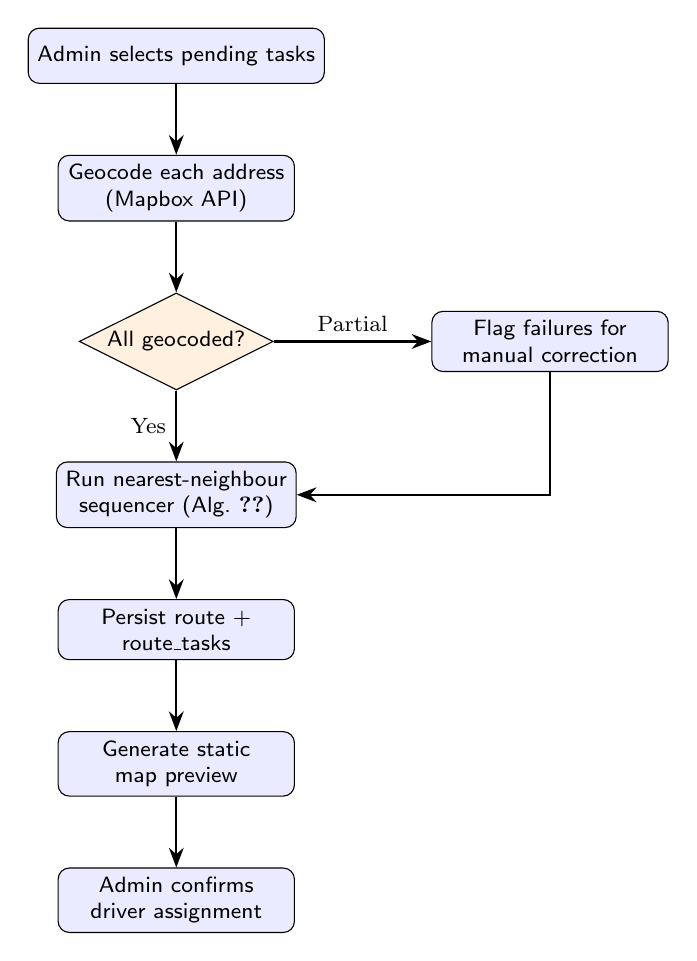
\begin{tikzpicture}[
    act/.style={draw, rounded corners=4pt, minimum width=3cm,
                minimum height=0.7cm, font=\sffamily\footnotesize,
                fill=blue!8, align=center},
    dec/.style={draw, diamond, aspect=2, inner sep=1pt,
                font=\sffamily\footnotesize, fill=orange!12},
    arr/.style={-{Stealth[length=2.5mm]}, thick},
    node distance=0.9cm
  ]
    \node[act]                     (start)  {Admin selects pending tasks};
    \node[act, below=of start]     (geo)    {Geocode each address\\(Mapbox API)};
    \node[dec, below=of geo]       (check)  {All geocoded?};
    \node[act, right=2cm of check] (skip)   {Flag failures for\\manual correction};
    \node[act, below=of check]     (nn)     {Run nearest-neighbour\\sequencer (Alg.~\ref{alg:nn})};
    \node[act, below=of nn]        (store)  {Persist route +\\route\_tasks};
    \node[act, below=of store]     (map)    {Generate static\\map preview};
    \node[act, below=of map]       (assign) {Admin confirms\\driver assignment};

    \draw[arr] (start)  -- (geo);
    \draw[arr] (geo)    -- (check);
    \draw[arr] (check)  -- node[left, font=\footnotesize]{Yes} (nn);
    \draw[arr] (check)  -- node[above, font=\footnotesize]{Partial} (skip);
    \draw[arr] (skip.south) |- (nn);
    \draw[arr] (nn)     -- (store);
    \draw[arr] (store)  -- (map);
    \draw[arr] (map)    -- (assign);
  \end{tikzpicture}}%
  \caption{Activity diagram for the route generation pipeline.}
  \label{fig:route-pipeline}
\end{figure}

\begin{algorithm}[ht]
  \caption{Greedy Nearest-Neighbour Route Sequencing}\label{alg:nn}
  \KwIn{Depot location $\mathbf{o}$; set of task locations $T = \{t_1, \dots, t_n\}$}
  \KwOut{Ordered sequence $S$}
  $S \leftarrow [\,]$\;
  $\mathit{current} \leftarrow \mathbf{o}$\;
  $R \leftarrow T$ \tcp*{remaining tasks}
  \While{$R \neq \emptyset$}{
    $t^* \leftarrow \arg\min_{t \in R}\; \textsc{Haversine}(\mathit{current},\; t)$\;
    Append $t^*$ to $S$\;
    $\mathit{current} \leftarrow t^*$\;
    $R \leftarrow R \setminus \{t^*\}$\;
  }
  \Return{$S$}\;
\end{algorithm}

The Haversine formula used in Algorithm~\ref{alg:nn} computes great-circle
distance:
\begin{equation}
  d = 2\,R_{\oplus}\;\arctan\!\Bigl(
    \sqrt{a},\; \sqrt{1-a}\Bigr),
  \quad
  a = \sin^{2}\!\frac{\Delta\phi}{2}
    + \cos\phi_1\,\cos\phi_2\;\sin^{2}\!\frac{\Delta\lambda}{2}
  \label{eq:haversine}
\end{equation}
where $R_{\oplus} = 6{,}371$\,km is the mean Earth radius, $\phi$ is
latitude, and $\lambda$ is longitude.  The implementation
(Listing~\ref{lst:haversine}) mirrors Equation~\ref{eq:haversine} directly.

\begin{lstlisting}[
  language=Java,
  caption={Haversine distance in Dart (\texttt{mapbox\_service.dart}).},
  label={lst:haversine},
  morekeywords={double, const, final, return}
]
double distanceTo(GeoPoint other) {
  const earthRadius = 6371.0; // km
  final dLat = _toRad(other.lat - lat);
  final dLng = _toRad(other.lng - lng);
  final a = sin(dLat/2) * sin(dLat/2) +
      cos(_toRad(lat)) * cos(_toRad(other.lat)) *
      sin(dLng/2) * sin(dLng/2);
  final c = 2 * atan2(sqrt(a), sqrt(1 - a));
  return earthRadius * c;
}
\end{lstlisting}

\paragraph{Complexity analysis.}
The greedy nearest-neighbour heuristic runs in $O(n^2)$ time, where $n$ is
the number of tasks.  While metaheuristics such as Ant Colony Optimisation
\autocite{dorigo1997ant} can yield shorter routes, the $O(n^2)$ cost is
acceptable for the typical task sets in last-mile delivery ($n < 50$) and,
critically, permits real-time mid-shift re-sequencing on a mobile device
without perceptible latency.

% ─────────────────────────────────────────────────────────────
\section{Dynamic Priority Recalculation}
\label{sec:priority-impl}

Task ordering is not solely distance-based.  A time-urgency bonus is added to
each task's base priority at sort time, ensuring that approaching time windows
are respected even when a closer but non-urgent task exists.

\begin{algorithm}[ht]
  \caption{Dynamic Priority with Time-Urgency Bonus}\label{alg:priority}
  \KwIn{Task $t$ with base priority $p$ and optional scheduled time $s$; current time $\mathit{now}$}
  \KwOut{Effective priority $p'$}
  \uIf{$t$ is delivered}{
    \Return{$p$}\;
  }
  \uIf{$s$ is null}{
    \Return{$p$}\;
  }
  $\Delta \leftarrow s - \mathit{now}$\;
  \uIf{$\Delta < 0$}{$\mathit{bonus} \leftarrow 50$ \tcp*{overdue}}
  \uElseIf{$\Delta \leq 30\,\text{min}$}{$\mathit{bonus} \leftarrow 30$ \tcp*{imminent}}
  \uElseIf{$\Delta \leq 60\,\text{min}$}{$\mathit{bonus} \leftarrow 20$}
  \uElseIf{$\Delta \leq 120\,\text{min}$}{$\mathit{bonus} \leftarrow 10$}
  \Else{$\mathit{bonus} \leftarrow 0$}
  \Return{$p + \mathit{bonus}$}\;
\end{algorithm}

The composite sort order used by the task list view model is:
(1)~status class (pending $>$ in-transit $>$ delivered),
(2)~effective priority (descending),
(3)~scheduled time (ascending),
(4)~stable tie-break by task ID.
This four-level comparator prevents task list flickering while still surfacing
urgent deliveries.

% ─────────────────────────────────────────────────────────────
\section{Driver Recommendation}
\label{sec:driver-rec}

When an admin generates a route, the system recommends the most suitable driver
using a composite score computed in a PostgreSQL function:

\begin{equation}
  \mathit{score} =
    \underbrace{w_a}_{\text{availability}}
    \times
    \underbrace{\frac{1}{1 + d_{\text{km}}}}_{\text{proximity}}
    \times
    \underbrace{\frac{1}{1 + n_{\text{tasks}}}}_{\text{workload}}
    \times
    \underbrace{\bigl(0.5 + 0.5 \cdot r_{\text{completion}}\bigr)}_{\text{performance}}
  \label{eq:rec-score}
\end{equation}

where $w_a \in \{0.5, 1.0\}$ is the availability weight, $d_{\text{km}}$ is
the PostGIS-computed distance from the driver's last known location to the task
cluster centroid, $n_{\text{tasks}}$ is the driver's current task count, and
$r_{\text{completion}}$ is the ratio of successfully delivered tasks to total
assigned tasks (historical).  The function is executed entirely within
PostgreSQL, leveraging PostGIS \texttt{ST\_Distance} for spatial computation
and avoiding a network round-trip for each candidate driver.

\paragraph{Alternatives considered.}
A client-side scoring approach was prototyped first but required fetching all
driver locations to the admin device.  Moving the computation server-side
reduced payload size and exploited PostGIS spatial indexes for sub-millisecond
distance queries.

% ─────────────────────────────────────────────────────────────
\section{Fleet-Wide Optimisation}
\label{sec:fleet-impl}

For dispatching multiple tasks across several drivers simultaneously, a greedy
nearest-driver assignment strategy is employed:

\begin{enumerate}
  \item Geocode all unassigned tasks.
  \item For each task, compute the Haversine distance to every available driver.
  \item Assign the task to the closest driver.
\end{enumerate}

This produces an $O(t \times d)$ assignment where $t$ is the number of tasks
and $d$ is the number of drivers.  While a Hungarian-algorithm assignment
would be globally optimal, the greedy approach was chosen because it runs in
real-time and the marginal optimality loss is negligible for small fleets
($d < 20$) typical of Hong Kong SMEs \autocite{toth2002vehicle}.

% ─────────────────────────────────────────────────────────────
\section{AI Integration}
\label{sec:ai-impl}

The AI subsystem comprises three modes of operation, each calling DeepSeek~R1
through the OpenRouter API \autocite{openrouter2026docs}.

\subsection{Task Summarisation}
\label{sec:ai-summary}

A compact system prompt instructs the model to summarise the driver's current
task list in under 160 tokens.  Temperature is set to $0.3$ to favour
deterministic, factual output.

\subsection{Free-Form Chat}
\label{sec:ai-chat}

A multi-turn chat interface injects the fleet context (task counts, route
status) as a system prompt, followed by the conversation history.  The model
responds with natural-language advice; tokens are capped at 200 to prevent
verbose answers.

\subsection{Agentic Suggestions}
\label{sec:ai-agentic}

The agentic mode extends the chat interface with a structured JSON action
schema.  The LLM is instructed to analyse the driver's situation and return a
JSON object containing a natural-language \texttt{suggestion} and an
executable \texttt{action} field from a predefined vocabulary:

\begin{center}
\small
\texttt{start\_next\_pending} \quad
\texttt{mark\_delivered} \quad
\texttt{go\_available} \quad
\texttt{go\_offline} \quad
\texttt{sync\_pending} \quad
\texttt{refresh\_tasks}
\end{center}

The client parses the JSON response and renders a one-tap confirmation chip.
Figure~\ref{fig:agentic-flow} shows the interaction sequence.

\begin{figure}[ht]
  \centering
  \resizebox{0.88\textwidth}{!}{%
  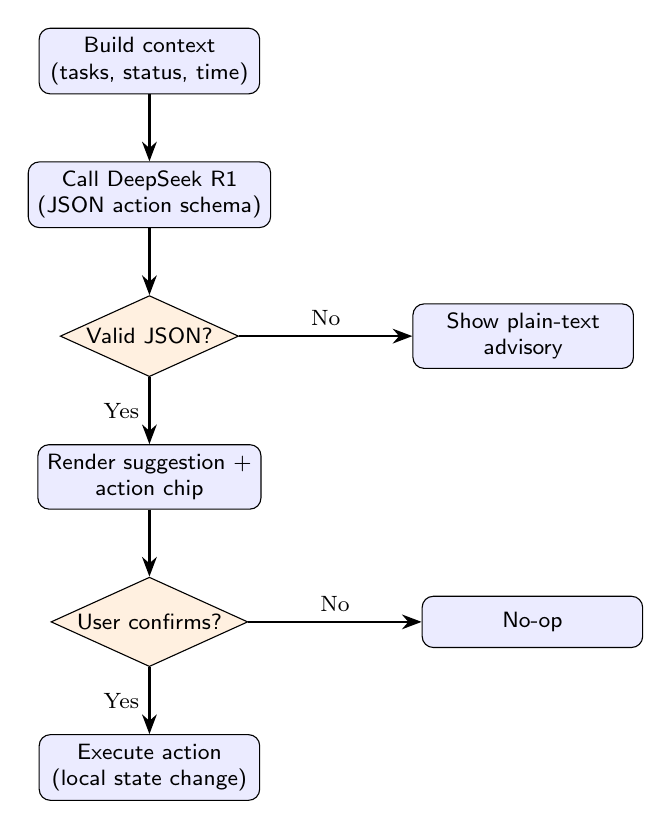
\begin{tikzpicture}[
    act/.style={draw, rounded corners=4pt, minimum width=2.8cm,
                minimum height=0.65cm, font=\sffamily\footnotesize,
                fill=blue!8, align=center},
    dec/.style={draw, diamond, aspect=2.2, inner sep=1pt,
                font=\sffamily\footnotesize, fill=orange!12, align=center},
    arr/.style={-{Stealth[length=2.5mm]}, thick},
    node distance=0.85cm
  ]
    \node[act]                     (ctx)   {Build context\\{(}tasks, status, time{)}};
    \node[act, below=of ctx]       (call)  {Call DeepSeek R1\\(JSON action schema)};
    \node[dec, below=of call]      (parse) {Valid JSON?};
    \node[act, below=of parse]     (chip)  {Render suggestion +\\action chip};
    \node[act, right=2.2cm of parse] (fallback) {Show plain-text\\advisory};
    \node[dec, below=of chip]      (tap)   {User confirms?};
    \node[act, below=of tap]       (exec)  {Execute action\\(local state change)};
    \node[act, right=2.2cm of tap] (ignore) {No-op};

    \draw[arr] (ctx)      -- (call);
    \draw[arr] (call)     -- (parse);
    \draw[arr] (parse)    -- node[left, font=\footnotesize]{Yes} (chip);
    \draw[arr] (parse)    -- node[above, font=\footnotesize]{No}  (fallback);
    \draw[arr] (chip)     -- (tap);
    \draw[arr] (tap)      -- node[left, font=\footnotesize]{Yes} (exec);
    \draw[arr] (tap)      -- node[above, font=\footnotesize]{No}  (ignore);
  \end{tikzpicture}}%
  \caption{Agentic AI suggestion flow with user confirmation gate.}
  \label{fig:agentic-flow}
\end{figure}

This human-in-the-loop design prevents the LLM from executing unintended
actions—a critical safeguard given that LLM outputs can hallucinate
\autocite{ji2024hallucination}.  Temperature is lowered to $0.2$ for the
agentic mode to maximise output predictability.

% ─────────────────────────────────────────────────────────────
\section{Proof-of-Delivery Workflow}
\label{sec:pod-impl}

Before a task can be marked as \emph{completed}, the driver must capture a
photo using the device camera.  The image is written to Supabase Storage with a
path derived from the task ID, and the public URL is written back to the
\texttt{tasks.proof\_photo\_url} column.  The admin portal displays the photo
in a review panel alongside the delivery address and completion timestamp.

An optional confirmation code (e.g.\ a PIN provided by the recipient) is
stored in \texttt{tasks.proof\_code}.  Both fields together form the proof
of delivery (PoD) bundle, which is auditable per task.

% ─────────────────────────────────────────────────────────────
\section{Offline Synchronisation}
\label{sec:sync-impl}

The offline sync mechanism (Figure~\ref{fig:sync}) ensures data durability in
areas with unreliable connectivity.

\begin{figure}[ht]
  \centering
  \resizebox{0.92\textwidth}{!}{%
  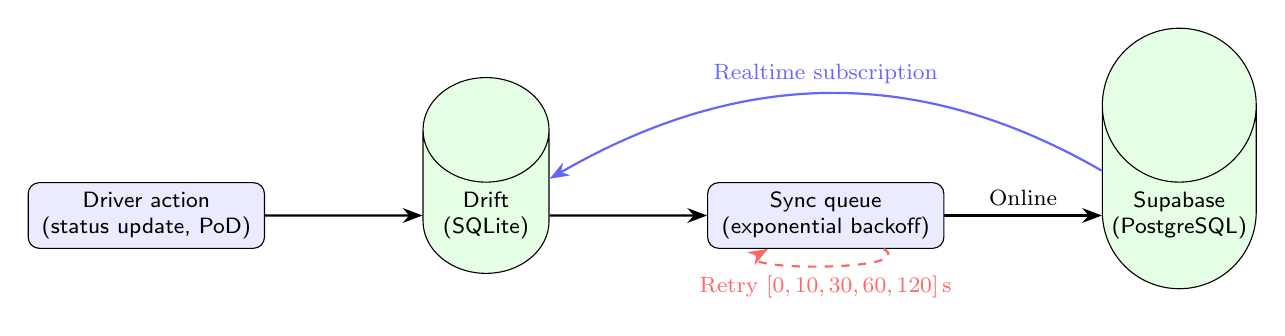
\begin{tikzpicture}[
    act/.style={draw, rounded corners=4pt, minimum width=3cm,
                minimum height=0.65cm, font=\sffamily\footnotesize,
                fill=blue!8, align=center},
    store/.style={draw, cylinder, shape border rotate=90,
                  minimum width=1.6cm, minimum height=0.8cm,
                  font=\sffamily\footnotesize, fill=green!10, align=center},
    arr/.style={-{Stealth[length=2.5mm]}, thick},
    darr/.style={-{Stealth[length=2.5mm]}, thick, dashed, red!60},
    node distance=1cm and 2cm
  ]
    \node[act]                         (write)  {Driver action\\(status update, PoD)};
    \node[store, right=of write]       (drift)  {Drift\\{(}SQLite{)}};
    \node[act, right=of drift]         (queue)  {Sync queue\\{(}exponential backoff{)}};
    \node[store, right=of queue]       (supa)   {Supabase\\{(}PostgreSQL{)}};

    \draw[arr]  (write) -- (drift);
    \draw[arr]  (drift) -- (queue);
    \draw[arr]  (queue) -- node[above, font=\footnotesize]{Online} (supa);
    \draw[darr] (queue) to[out=-30,in=-150] node[below, font=\footnotesize]{Retry [0,\,10,\,30,\,60,\,120]\,s} (queue);

    % Realtime path back
    \draw[arr, blue!60] (supa) to[out=150,in=30]
      node[above, font=\footnotesize, blue!60]{Realtime subscription} (drift);
  \end{tikzpicture}}%
  \caption{Offline synchronisation with exponential-backoff retry and Realtime reconciliation.}
  \label{fig:sync}
\end{figure}

\begin{enumerate}
  \item Every write first persists to the local Drift database (immediate UI
        feedback).
  \item The mutation is enqueued into \texttt{sync\_queue\_items} with
        \texttt{status = 'pending'}.
  \item A background isolate dequeues items and attempts upload.  On failure,
        \texttt{attempts} is incremented and \texttt{last\_attempt\_at} is
        updated; the next retry is delayed according to a progressive
        schedule $[0, 10, 30, 60, 120]$~seconds.  After five failed attempts
        the item is marked as permanently failed.
  \item On reconnection, Supabase Realtime pushes server-side changes;
        conflicts are resolved by comparing \texttt{updated\_at} timestamps
        (last-writer-wins).
\end{enumerate}

% ─────────────────────────────────────────────────────────────
\section{Admin Portal}
\label{sec:admin-impl}

The admin portal is implemented as a role-gated view within the same Flutter
application.  Key screens include:

\begin{itemize}
  \item \textbf{Task Management} — CRUD operations with inline validation;
        bulk CSV import parses headers (\texttt{address}, \texttt{notes},
        \texttt{priority}, \texttt{scheduled\_start}, \texttt{scheduled\_end})
        and rejects malformed rows with error feedback.
  \item \textbf{Route Dashboard} — displays generated routes on a Mapbox
        static-map tile with sequenced stop markers; shows total distance and
        recommended driver.
  \item \textbf{Fleet Monitor} — real-time driver locations plotted on a map
        via Supabase Realtime subscriptions to the \texttt{company\_members}
        table (which stores \texttt{last\_known\_location}).
  \item \textbf{PoD Review} — photo and signature viewer per task, with
        accept/reject controls.
  \item \textbf{Chat} — admin-to-driver messaging with broadcast support.
\end{itemize}

% ─────────────────────────────────────────────────────────────
\section{Mid-Shift Re-Sequencing}
\label{sec:reseq-impl}

When conditions change after a route has been dispatched (e.g.\ a task is
cancelled or traffic reroutes the driver), the system can re-sequence the
remaining tasks from the driver's \emph{current GPS position} rather than the
original depot.  The existing nearest-neighbour sequencer
(Algorithm~\ref{alg:nn}) is re-invoked with the driver's live coordinates as
the origin, and only undelivered tasks are included.  The result is stored as
a temporary client-side ordering override that expires after one hour,
preventing stale overrides from persisting across shifts.

% ─────────────────────────────────────────────────────────────
\section{Barcode and QR-Code Scanner}
\label{sec:barcode-impl}

Drivers can scan a barcode or QR code affixed to a parcel to instantly locate
the corresponding task in their list.  The feature is implemented as a
\texttt{BarcodeScannerSheet}—a reusable bottom-sheet widget backed by the
\texttt{mobile\_scanner} package, which accesses the device camera and
performs real-time barcode detection.

The interaction proceeds as follows:

\begin{enumerate}
  \item The driver taps the scan icon on the task list toolbar.
  \item A bottom sheet opens containing a live camera preview
        (\texttt{MobileScanner} widget).
  \item On detection, a debounce flag (\texttt{\_hasResult}) prevents
        duplicate scans; the first valid code is trimmed and returned via
        \texttt{Navigator.pop(value)}.
  \item The calling screen receives the scanned string and filters the task
        list to the matching delivery.
\end{enumerate}

This eliminates the need for manual task lookup when parcels carry
machine-readable labels—a common workflow in Hong Kong logistics depots
where hundreds of parcels are handled per shift.

% ─────────────────────────────────────────────────────────────
\section{Customer Tracking Lookup}
\label{sec:tracking-impl}

The admin portal includes a customer-facing tracking lookup that allows
administrators—or, in a future extension, end-customers directly—to query
delivery status using a human-readable tracking code (format
\texttt{OV-ABC1-XYZ2}).

\subsection{Implementation}

The lookup is implemented via a Supabase RPC call to the
\texttt{lookup\_delivery\_by\_tracking} PostgreSQL function, which accepts a
single parameter \texttt{p\_tracking\_code} and returns a JSON object
containing:

\begin{itemize}
  \item \texttt{found} — boolean indicating whether a matching delivery exists,
  \item \texttt{status} — current task state (pending / in-transit / delivered),
  \item \texttt{address} — delivery address,
  \item \texttt{driver\_assigned} — name of the assigned driver,
  \item \texttt{proof\_available} — boolean indicating whether PoD has been captured,
  \item \texttt{last\_update} — ISO-8601 timestamp of the most recent status change.
\end{itemize}

The UI renders the result in a colour-coded card: green for delivered, blue for
in-transit, and orange for pending.  Error states (no match, network failure)
are presented as inline messages, keeping the admin within the same screen
context.

% Chapter 5: Testing and Evaluation
\chapter{Testing and Evaluation}
\label{ch:testing}

This chapter presents the testing strategy, functional test results, security
verification, route-optimisation evaluation, AI evaluation, and a mapping of
results against the fourteen project objectives defined in
Section~\ref{sec:objectives}.  All testing was performed by a single developer
using a physical Android device (Samsung Galaxy A54, Android~14) and the Chrome
desktop browser, reflecting the realistic constraints of an academic project.

% ─────────────────────────────────────────────────────────────
\section{Testing Strategy}
\label{sec:test-strategy}

Testing was organised into four tiers:

\begin{enumerate}
  \item \textbf{Unit tests}: automated Dart tests targeting the
        \texttt{TaskViewModel} business logic (task loading, offline queuing,
        sync recovery).
  \item \textbf{Functional tests}: manual end-to-end walkthroughs of every
        user-facing feature, recorded in Table~\ref{tab:func-admin} (admin)
        and Table~\ref{tab:func-driver} (driver).
  \item \textbf{Security tests}: cross-tenant Row-Level Security (RLS)
        verification and RBAC enforcement.
  \item \textbf{Quantitative evaluation}: route-optimisation distance
        measurements, AI response-quality assessment, and driver-recommendation
        accuracy.
\end{enumerate}

\noindent Figure~\ref{fig:test-pyramid} visualises how these four tiers build
upon one another, with the broadest automated coverage at the base narrowing
towards the quantitative evaluation at the apex.

\begin{figure}[H]
  \centering
  \resizebox{0.82\textwidth}{!}{%
  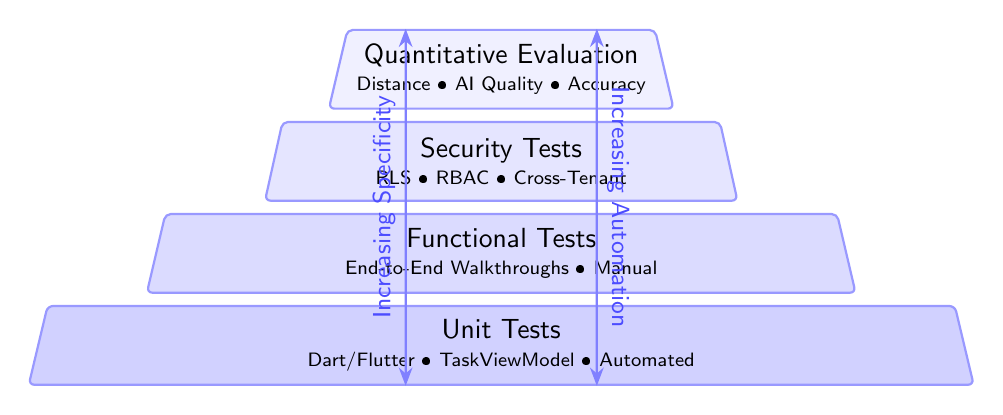
\begin{tikzpicture}[
      >=Stealth,
      every node/.style={font=\sffamily},
      layer/.style={
        trapezium, trapezium angle=75,
        draw=blue!40, thick, rounded corners=2pt,
        text=black, minimum height=1cm,
        trapezium stretches body,
        align=center
      }
    ]
    % Layers from bottom (widest) to top (narrowest)
    \node[layer, fill=blue!18, minimum width=12cm]
      (unit) {Unit Tests\\[-2pt]{\scriptsize Dart/Flutter \textbullet{} TaskViewModel \textbullet{} Automated}};
    \node[layer, fill=blue!14, minimum width=9cm, above=4pt of unit]
      (func) {Functional Tests\\[-2pt]{\scriptsize End-to-End Walkthroughs \textbullet{} Manual}};
    \node[layer, fill=blue!10, minimum width=6cm, above=4pt of func]
      (sec)  {Security Tests\\[-2pt]{\scriptsize RLS \textbullet{} RBAC \textbullet{} Cross-Tenant}};
    \node[layer, fill=blue!6, minimum width=3.5cm, above=4pt of sec]
      (quant){Quantitative Evaluation\\[-2pt]{\scriptsize Distance \textbullet{} AI Quality \textbullet{} Accuracy}};

    % Side annotations
    \draw[<->, thick, blue!50] ([xshift=-7mm]unit.south west)
      -- node[left, rotate=90, anchor=south, font=\sffamily\small, blue!70]
         {Increasing Specificity} ([xshift=-7mm]quant.north west);
    \draw[<->, thick, blue!50] ([xshift=7mm]unit.south east)
      -- node[right, rotate=-90, anchor=south, font=\sffamily\small, blue!70]
         {Increasing Automation} ([xshift=7mm]quant.north east);
  \end{tikzpicture}%
  }%
  \caption{Testing strategy pyramid: four tiers from broad automated
           unit coverage to focused quantitative evaluation.}
  \label{fig:test-pyramid}
\end{figure}

% ─────────────────────────────────────────────────────────────
\section{Unit Tests}
\label{sec:unit-tests}

Two automated unit tests validate the \texttt{TaskViewModel} using a
\texttt{\_FakeTaskRepository} that wraps an in-memory Drift database:

\begin{enumerate}
  \item \textbf{loadTasks}: seeds the repository, calls
        \texttt{viewModel.loadTasks()}, and asserts that the task list is
        non-empty and \texttt{isOffline} is \texttt{false}.
  \item \textbf{markAsDelivered (offline queue)}: configures the fake
        repository to simulate offline mode, marks a task as delivered with a
        proof code, asserts that \texttt{isOffline} becomes \texttt{true} and
        \texttt{pendingSyncCount} increments, then calls
        \texttt{syncPendingDeliveries()} and verifies the count returns to
        zero.
\end{enumerate}

\noindent Both tests pass under \texttt{flutter test} on the project CI
pipeline.

% ─────────────────────────────────────────────────────────────
\section{Functional Testing: Admin Portal}
\label{sec:func-admin}

Table~\ref{tab:func-admin} lists the admin-side functional test cases.  Each
test was executed manually through the Chrome web interface and verified
against the expected outcome.

\begin{longtable}{c p{3.4cm} p{4.2cm} c c}
  \caption{Admin portal functional test cases.}
  \label{tab:func-admin} \\
  \toprule
  \textbf{ID} & \textbf{Test Case} & \textbf{Expected Result} & \textbf{Pass} & \textbf{Fig.} \\
  \midrule
  \endfirsthead
  \toprule
  \textbf{ID} & \textbf{Test Case} & \textbf{Expected Result} & \textbf{Pass} & \textbf{Fig.} \\
  \midrule
  \endhead
  \midrule
  \multicolumn{5}{r}{\footnotesize\itshape Continued on next page} \\
  \endfoot
  \bottomrule
  \endlastfoot

  A1 & Login with admin credentials
     & Dashboard displayed with task list and navigation
     & \checkmark
     & \ref{fig:ss-a1} \\

  A2 & Create a new task (manual entry)
     & Task appears in list with status \emph{pending}
     & \checkmark
     & \ref{fig:ss-a2} \\

  A3 & Import tasks via CSV upload
     & All valid rows created; malformed rows rejected with error message
     & \checkmark
     & \ref{fig:ss-a3} \\

  A4 & Edit an existing task
     & Changes saved; updated fields visible on refresh
     & \checkmark
     & \ref{fig:ss-a4} \\

  A5 & Delete a task
     & Task removed from list; database row deleted
     & \checkmark
     & \ref{fig:ss-a5} \\

  A6 & Generate route (nearest-neighbour)
     & Route created with sequenced stops; map preview displayed
     & \checkmark
     & \ref{fig:ss-a6} \\

  A7 & View driver recommendation scores
     & Drivers ranked by composite score; availability, distance, and performance shown
     & \checkmark
     & \ref{fig:ss-a7} \\

  A8 & Fleet-wide optimisation
     & Tasks assigned to nearest available drivers; assignments table shown
     & \checkmark
     & \ref{fig:ss-a8} \\

  A9 & Review proof-of-delivery photo
     & PoD image and metadata displayed in review panel
     & \checkmark
     & \ref{fig:ss-a9} \\

  A10 & Send chat message to driver
      & Message appears in driver's chat; read receipt tracked
      & \checkmark
      & \ref{fig:ss-a10} \\

  A11 & Send broadcast message
      & All drivers in company receive the message
      & \checkmark
      & \ref{fig:ss-a11} \\

  A12 & AI summary (admin view)
      & Natural-language summary of fleet status displayed
      & \checkmark
      & \ref{fig:ss-a12} \\

  A13 & Customer tracking lookup (valid code)
      & Delivery status card displayed with address, driver, and PoD flag
      & \checkmark
      & --- \\

  A14 & Customer tracking lookup (invalid code)
      & Inline warning ``No delivery found'' displayed
      & \checkmark
      & --- \\
\end{longtable}

% ── Screenshot placeholders — Admin ──

\begin{figure}[H]
  \centering
  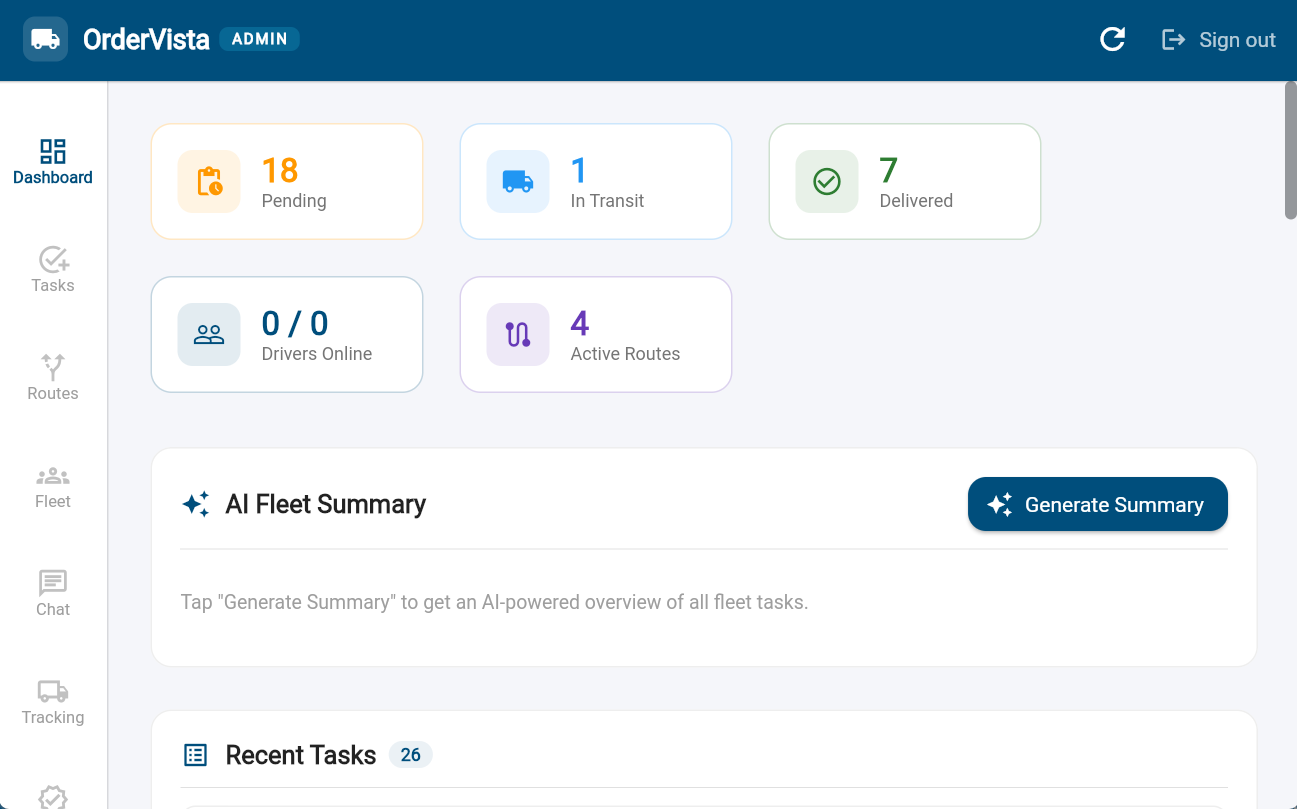
\includegraphics[width=0.7\textwidth]{ss-a1}
  \caption{Admin dashboard after login (A1).}
  \label{fig:ss-a1}
\end{figure}

\begin{figure}[H]
  \centering
  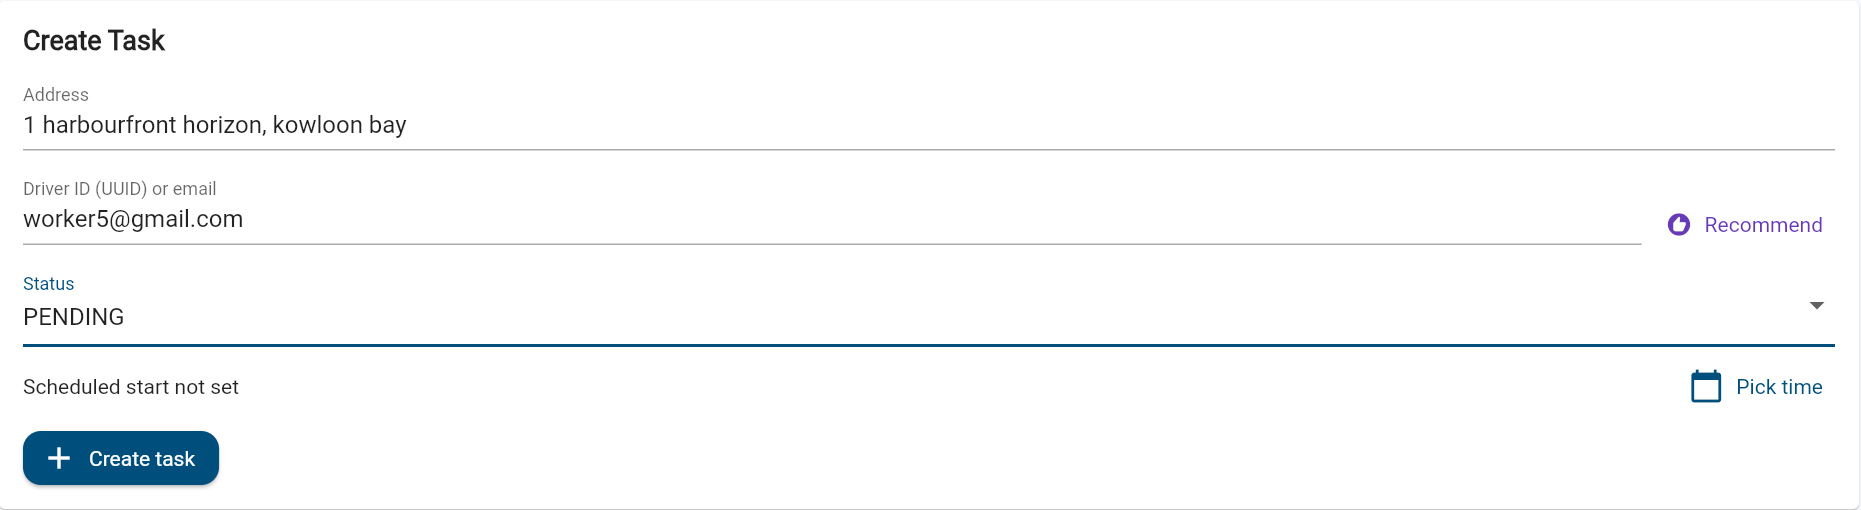
\includegraphics[width=0.7\textwidth]{ss-a2}
  \caption{Manual task creation form (A2).}
  \label{fig:ss-a2}
\end{figure}

\begin{figure}[H]
  \centering
  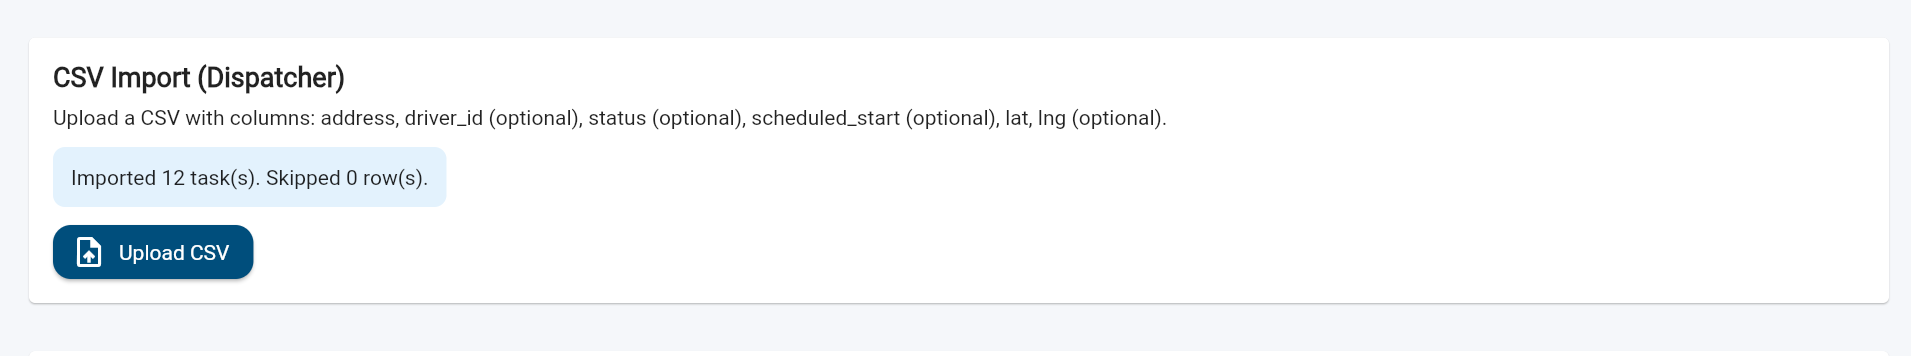
\includegraphics[width=0.7\textwidth]{ss-a3}
  \caption{CSV bulk import with error feedback (A3).}
  \label{fig:ss-a3}
\end{figure}

\begin{figure}[H]
  \centering
  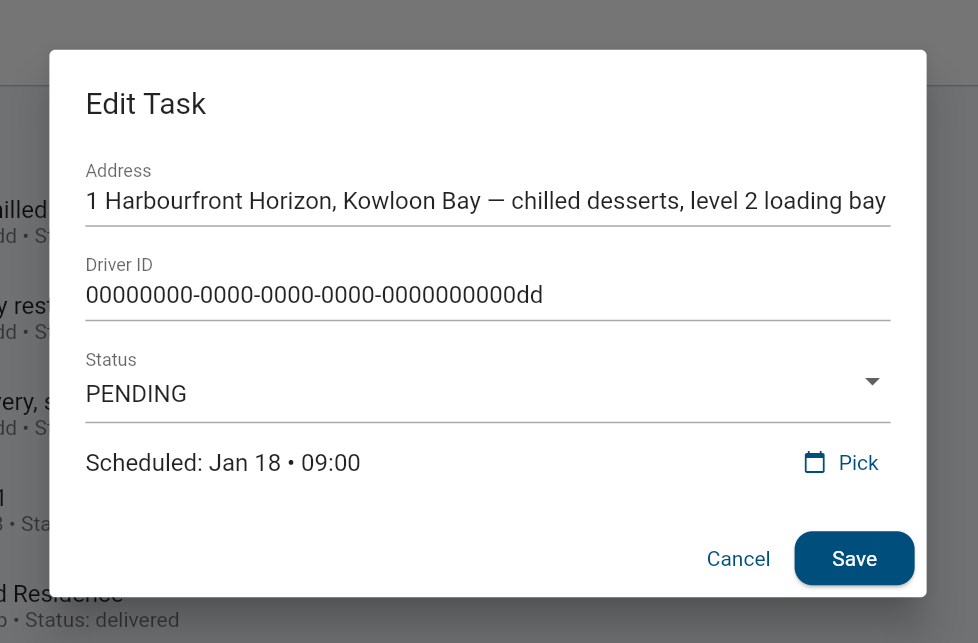
\includegraphics[width=0.7\textwidth]{ss-a4}
  \caption{Editing an existing task (A4).}
  \label{fig:ss-a4}
\end{figure}

\begin{figure}[H]
  \centering
  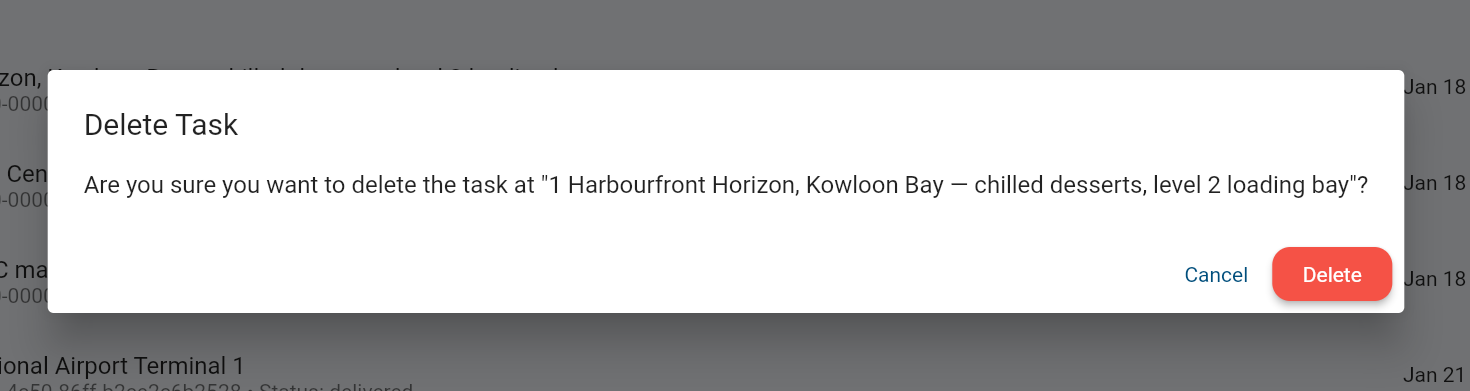
\includegraphics[width=0.7\textwidth]{ss-a5}
  \caption{Task deletion confirmation (A5).}
  \label{fig:ss-a5}
\end{figure}

\begin{figure}[H]
  \centering
  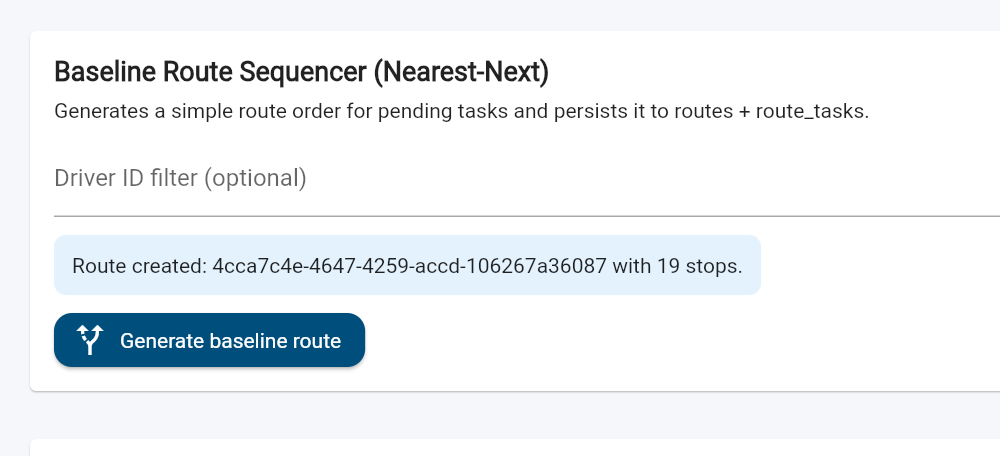
\includegraphics[width=0.7\textwidth]{ss-a6}
  \caption{Route generation with static map preview (A6).}
  \label{fig:ss-a6}
\end{figure}

\begin{figure}[H]
  \centering
  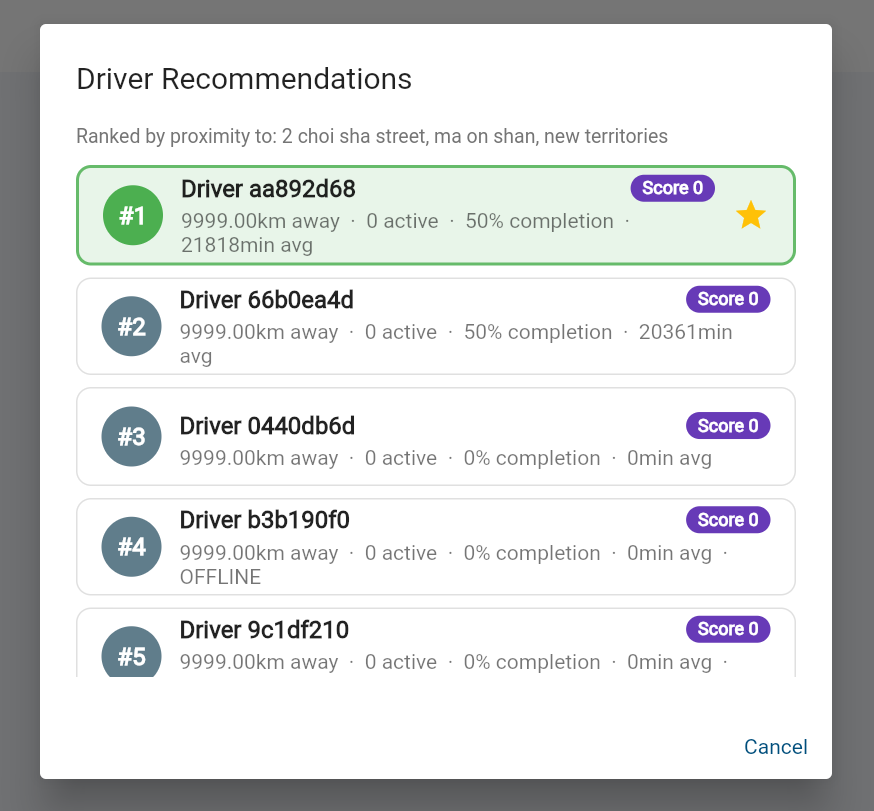
\includegraphics[width=0.7\textwidth]{ss-a7}
  \caption{Driver recommendation scores (A7).}
  \label{fig:ss-a7}
\end{figure}

\begin{figure}[H]
  \centering
  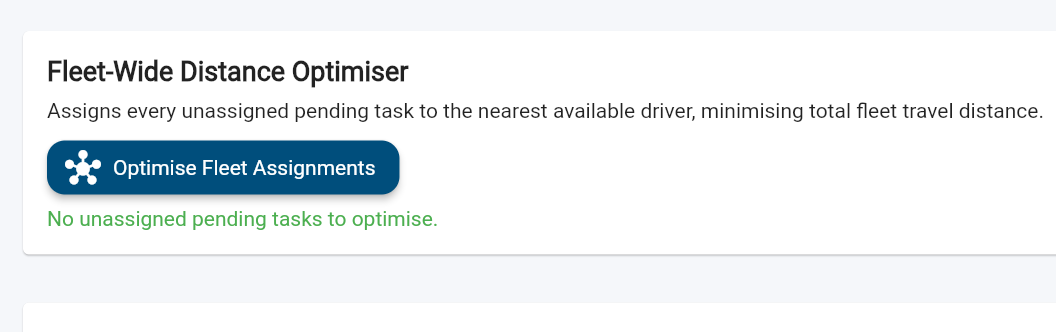
\includegraphics[width=0.7\textwidth]{ss-a8}
  \caption{Fleet-wide optimisation assignments (A8).}
  \label{fig:ss-a8}
\end{figure}

\begin{figure}[H]
  \centering
  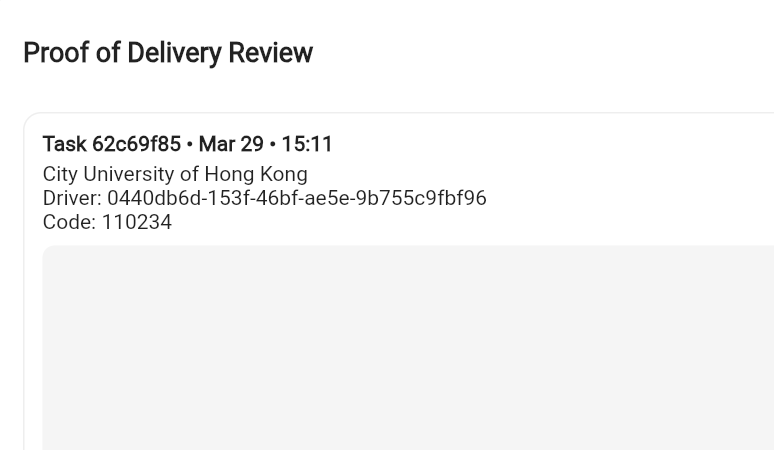
\includegraphics[width=0.7\textwidth]{ss-a9}
  \caption{Proof-of-delivery review panel (A9).}
  \label{fig:ss-a9}
\end{figure}

\begin{figure}[H]
  \centering
  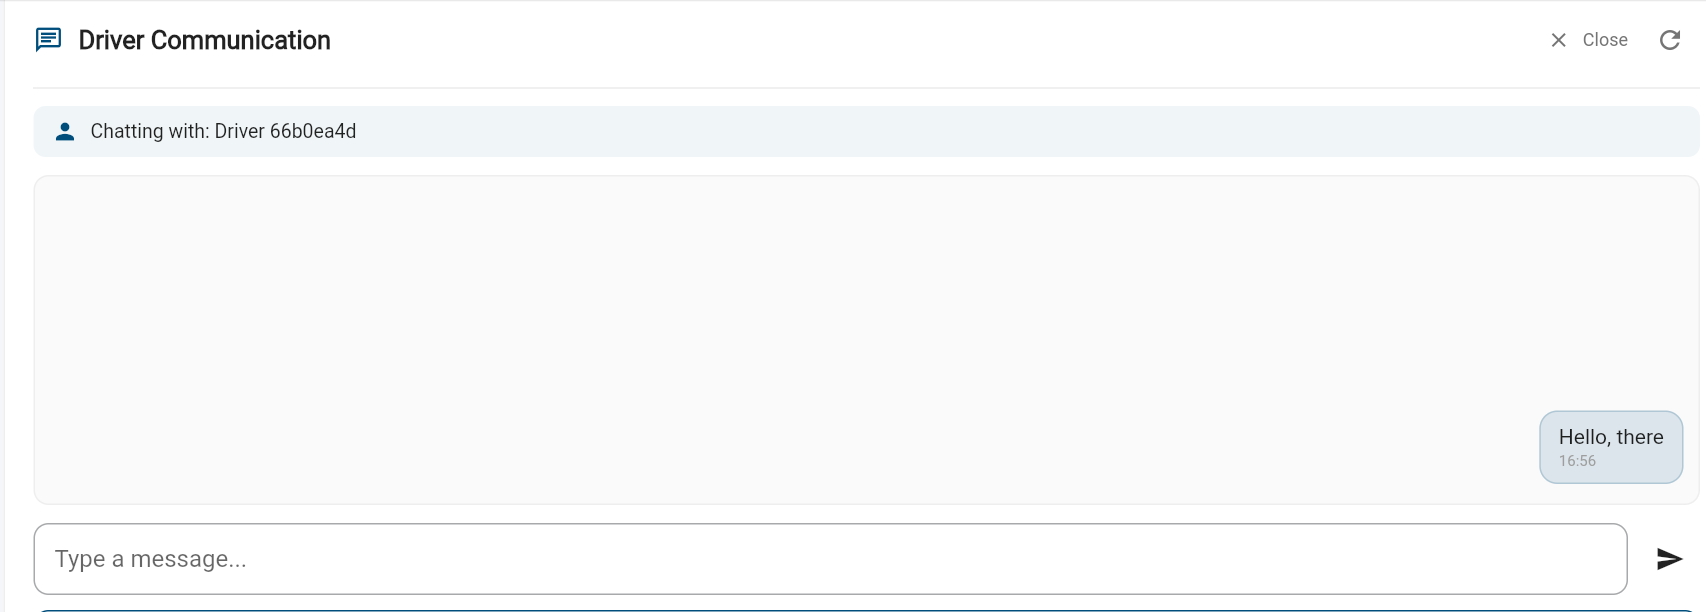
\includegraphics[width=0.7\textwidth]{ss-a10}
  \caption{Admin-to-driver chat message (A10).}
  \label{fig:ss-a10}
\end{figure}

\begin{figure}[H]
  \centering
  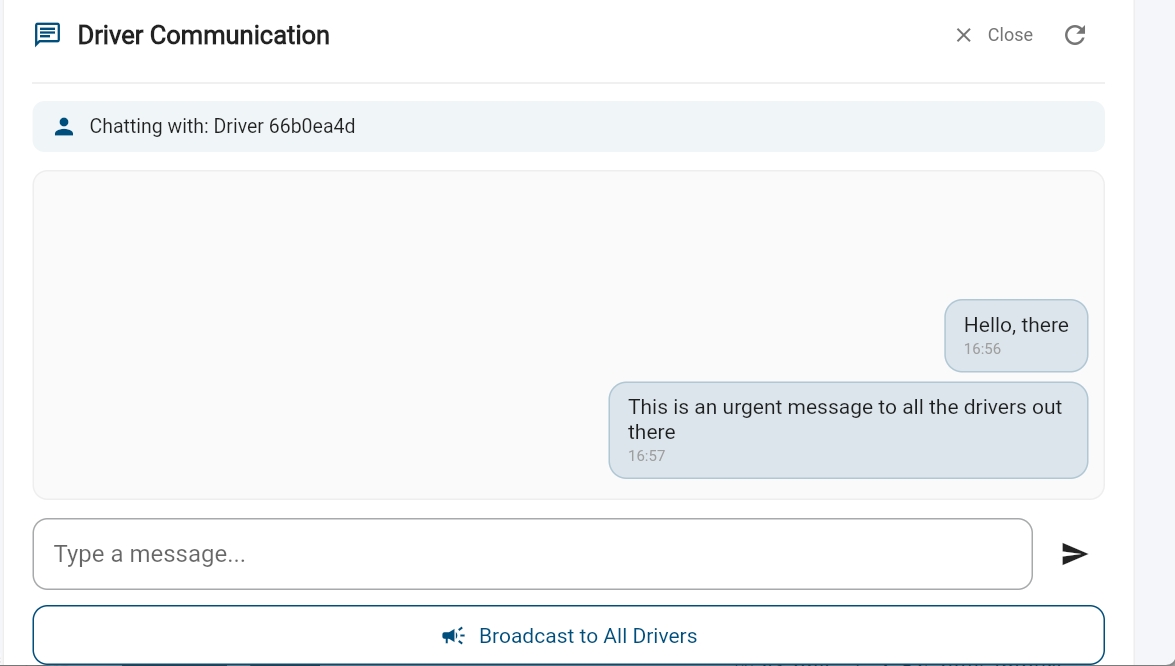
\includegraphics[width=0.7\textwidth]{ss-a11}
  \caption{Broadcast message to all drivers (A11).}
  \label{fig:ss-a11}
\end{figure}

\begin{figure}[H]
  \centering
  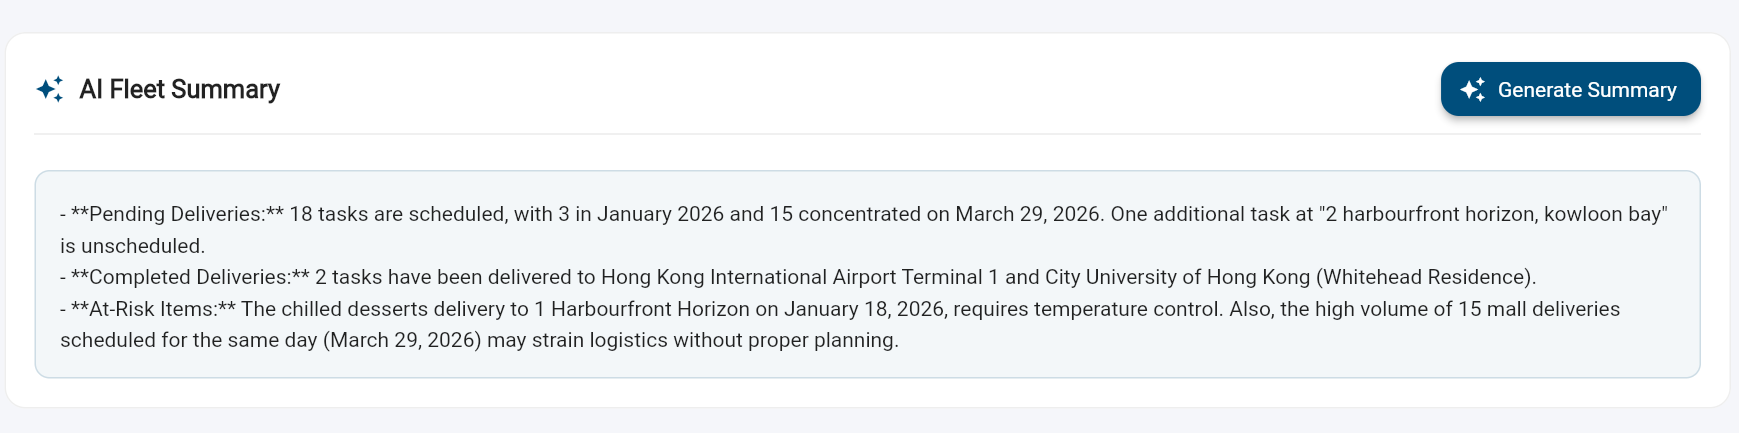
\includegraphics[width=0.7\textwidth]{ss-a12}
  \caption{AI-generated fleet summary (A12).}
  \label{fig:ss-a12}
\end{figure}

\clearpage
% ─────────────────────────────────────────────────────────────
\section{Functional Testing: Driver Application}
\label{sec:func-driver}

Table~\ref{tab:func-driver} lists the driver-side test cases executed on the
physical Samsung Galaxy~A54 device.

\begin{longtable}{c p{3.4cm} p{4.2cm} c c}
  \caption{Driver application functional test cases.}
  \label{tab:func-driver} \\
  \toprule
  \textbf{ID} & \textbf{Test Case} & \textbf{Expected Result} & \textbf{Pass} & \textbf{Fig.} \\
  \midrule
  \endfirsthead
  \toprule
  \textbf{ID} & \textbf{Test Case} & \textbf{Expected Result} & \textbf{Pass} & \textbf{Fig.} \\
  \midrule
  \endhead
  \midrule
  \multicolumn{5}{r}{\footnotesize\itshape Continued on next page} \\
  \endfoot
  \bottomrule
  \endlastfoot

  D1 & Login with driver credentials
     & Task list displayed with assigned deliveries
     & \checkmark
     & \ref{fig:ss-d1} \\

  D2 & View task details
     & Address, notes, priority, and time window shown
     & \checkmark
     & \ref{fig:ss-d2} \\

  D3 & Mark task as in-transit
     & Status badge updates to \emph{in-transit} in real-time
     & \checkmark
     & \ref{fig:ss-d3} \\

  D4 & Capture proof-of-delivery photo
     & Camera opens; photo uploaded to Supabase Storage; URL saved to task
     & \checkmark
     & \ref{fig:ss-d4} \\

  D5 & Mark task as delivered (with PoD)
     & Task moves to \emph{delivered}; PoD photo visible in admin review
     & \checkmark
     & \ref{fig:ss-d5} \\

  D6 & AI task summary
     & Natural-language summary of remaining tasks displayed
     & \checkmark
     & \ref{fig:ss-d6} \\

  D7 & AI chat (free-form question)
     & Contextual response returned within 3 seconds
     & \checkmark
     & \ref{fig:ss-d7} \\

  D8 & Agentic AI suggestion
     & Structured suggestion with one-tap action chip displayed
     & \checkmark
     & \ref{fig:ss-d8} \\

  D9 & Execute agentic action (confirm)
     & Action executed (e.g.\ task status changed); confirmation shown
     & \checkmark
     & \ref{fig:ss-d9} \\

  D10 & Mid-shift re-sequencing
      & Task order updates based on current GPS; resequence banner shown
      & \checkmark
      & \ref{fig:ss-d10} \\

  D11 & Offline delivery completion
      & Task marked delivered locally; sync icon appears; uploads on reconnect
      & \checkmark
      & \ref{fig:ss-d11} \\

  D12 & Receive chat message from admin
      & Message appears in chat tab; notification badge shown
      & \checkmark
      & \ref{fig:ss-d12} \\

  D13 & Toggle availability status
      & Status updates to available/offline; admin sees change in real-time
      & \checkmark
      & \ref{fig:ss-d13} \\

  D14 & Sign out
      & Session ended; login screen shown
      & \checkmark
      & \ref{fig:ss-d14} \\

  D15 & Scan barcode to locate task
      & Camera opens; scanned code matches task; task highlighted in list
      & \checkmark
      & --- \\
\end{longtable}

% ── Screenshot placeholders — Driver ──

\begin{figure}[H]
  \centering
  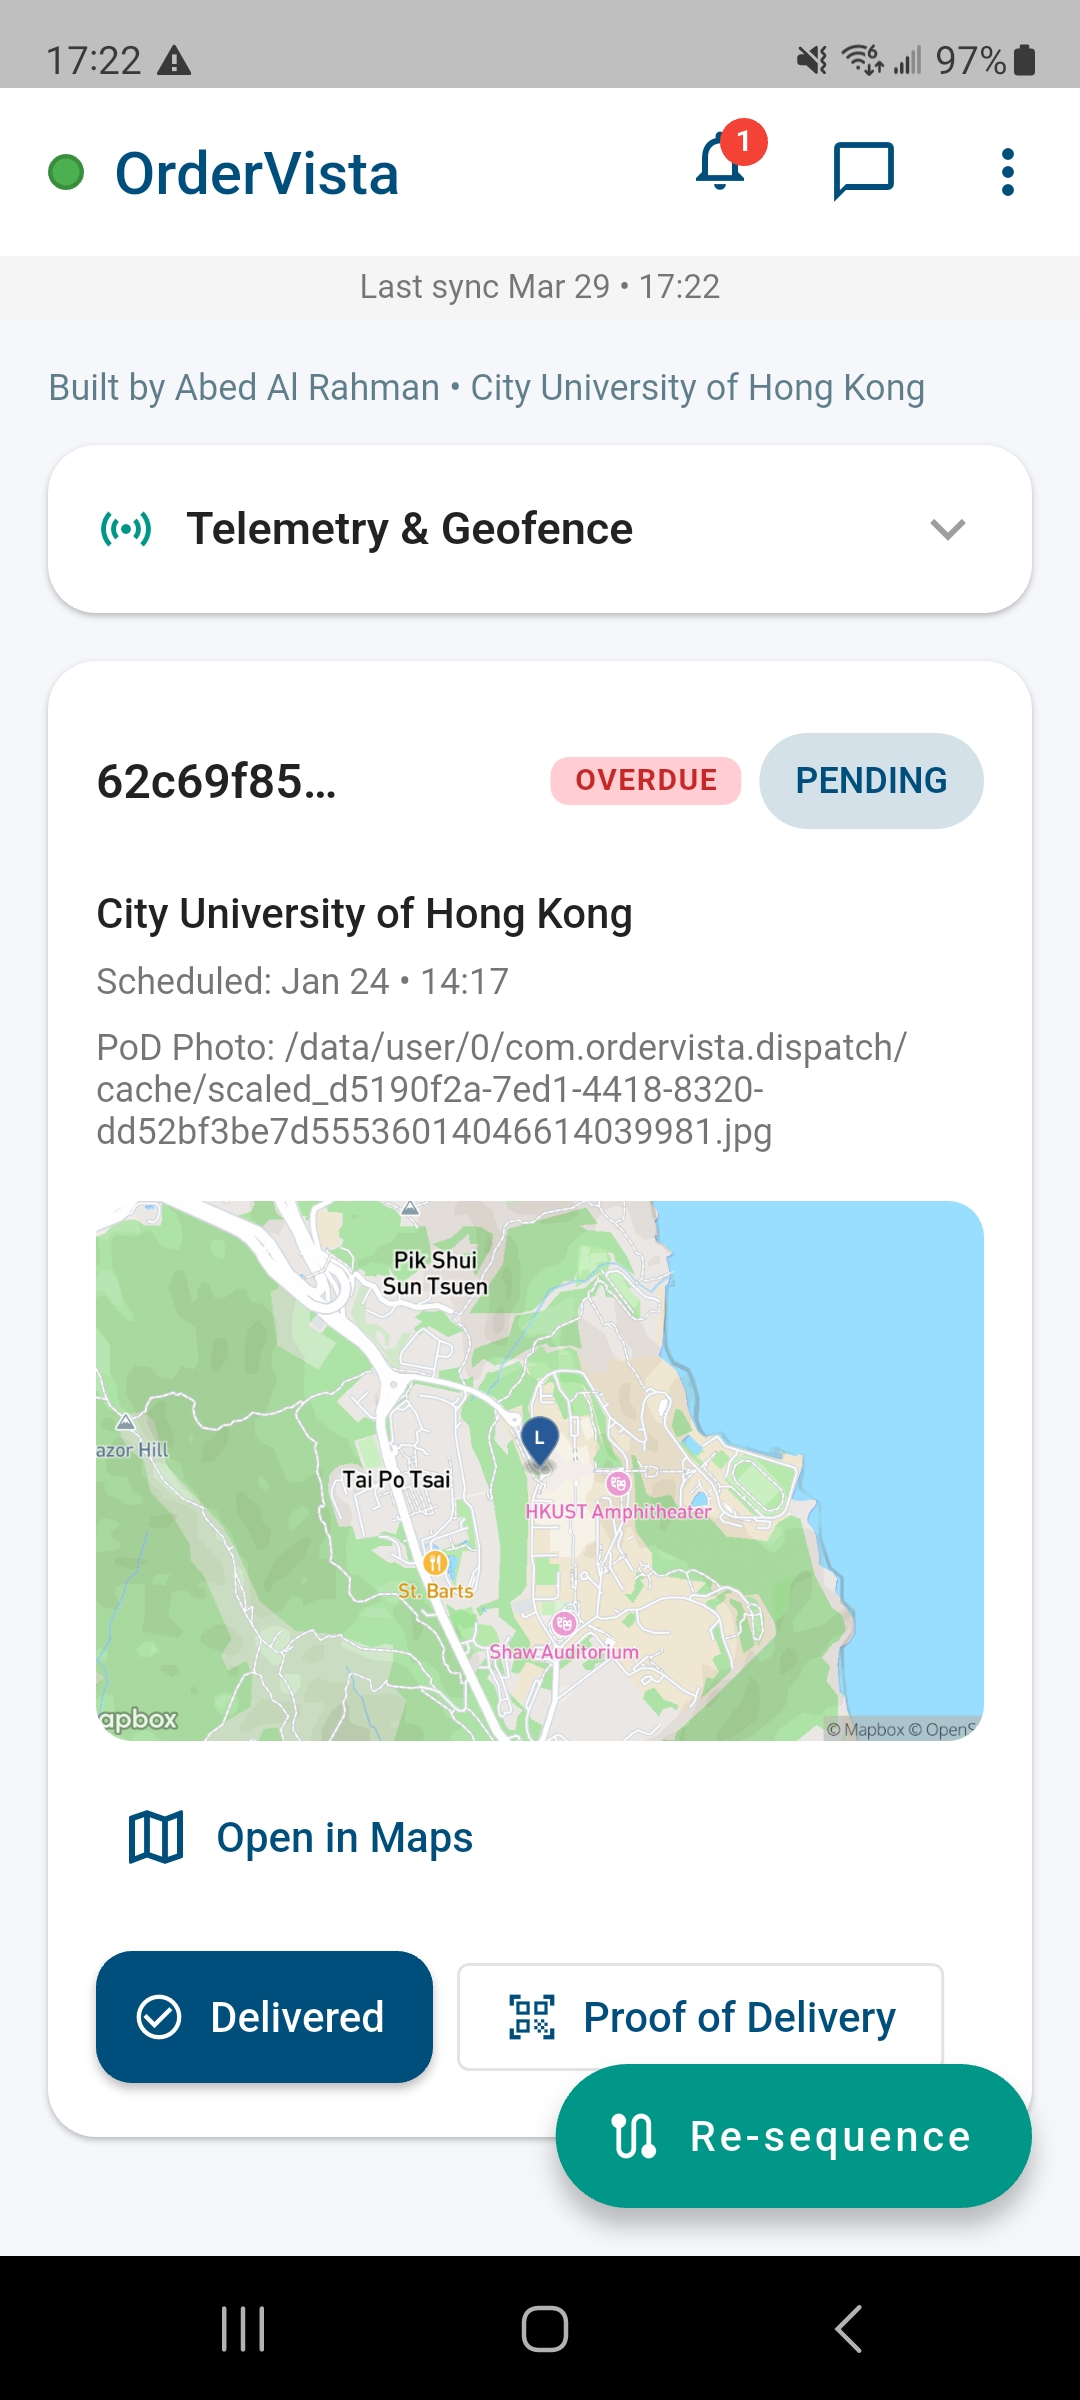
\includegraphics[width=0.45\textwidth]{ss-d1}
  \caption{Driver login screen (D1).}
  \label{fig:ss-d1}
\end{figure}

\begin{figure}[H]
  \centering
  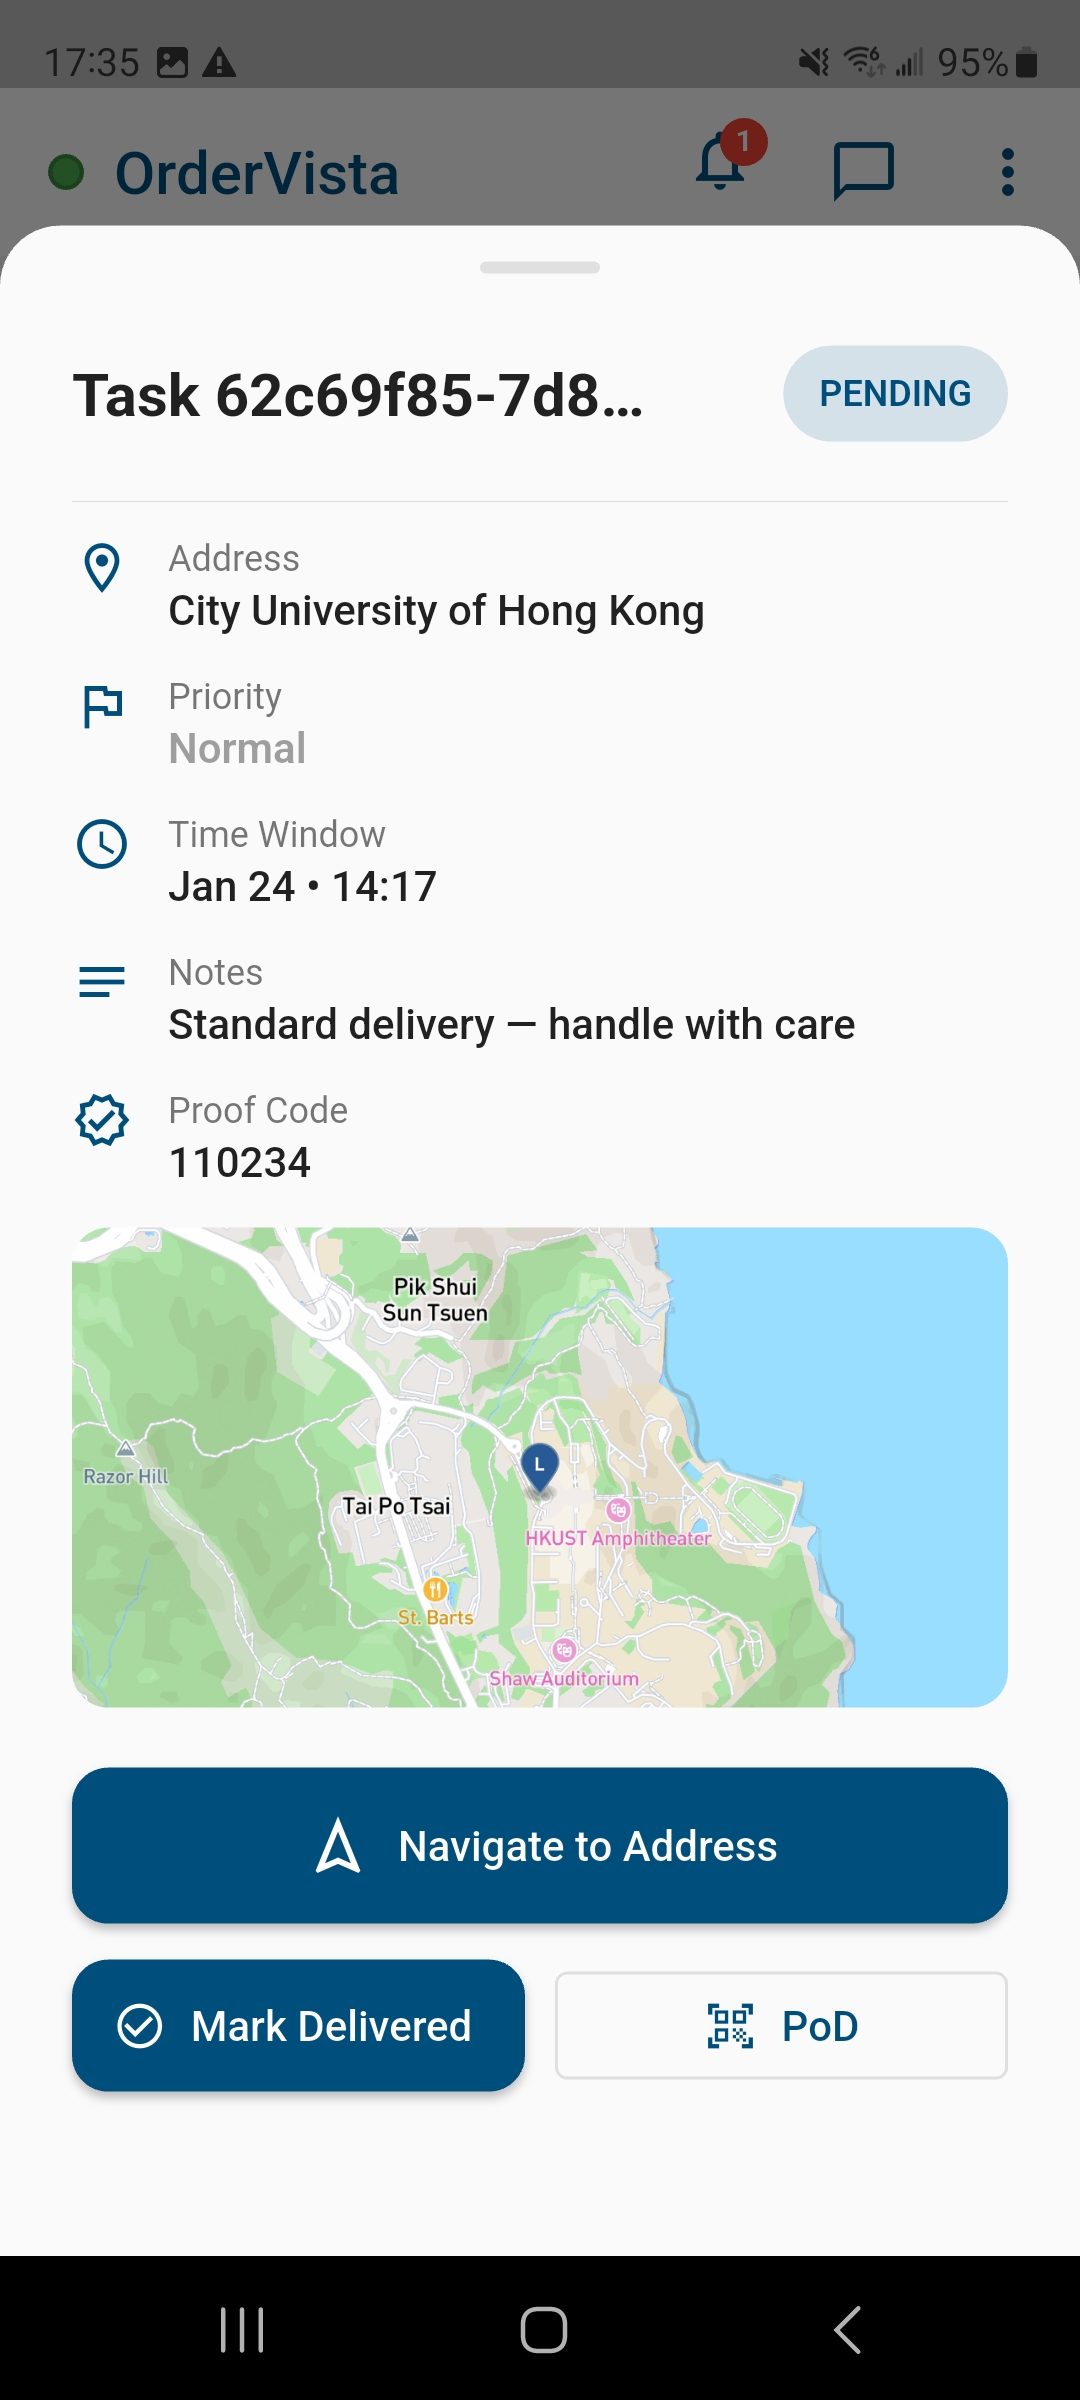
\includegraphics[width=0.45\textwidth]{ss-d2}
  \caption{Task detail view with address and time window (D2).}
  \label{fig:ss-d2}
\end{figure}

\begin{figure}[H]
  \centering
  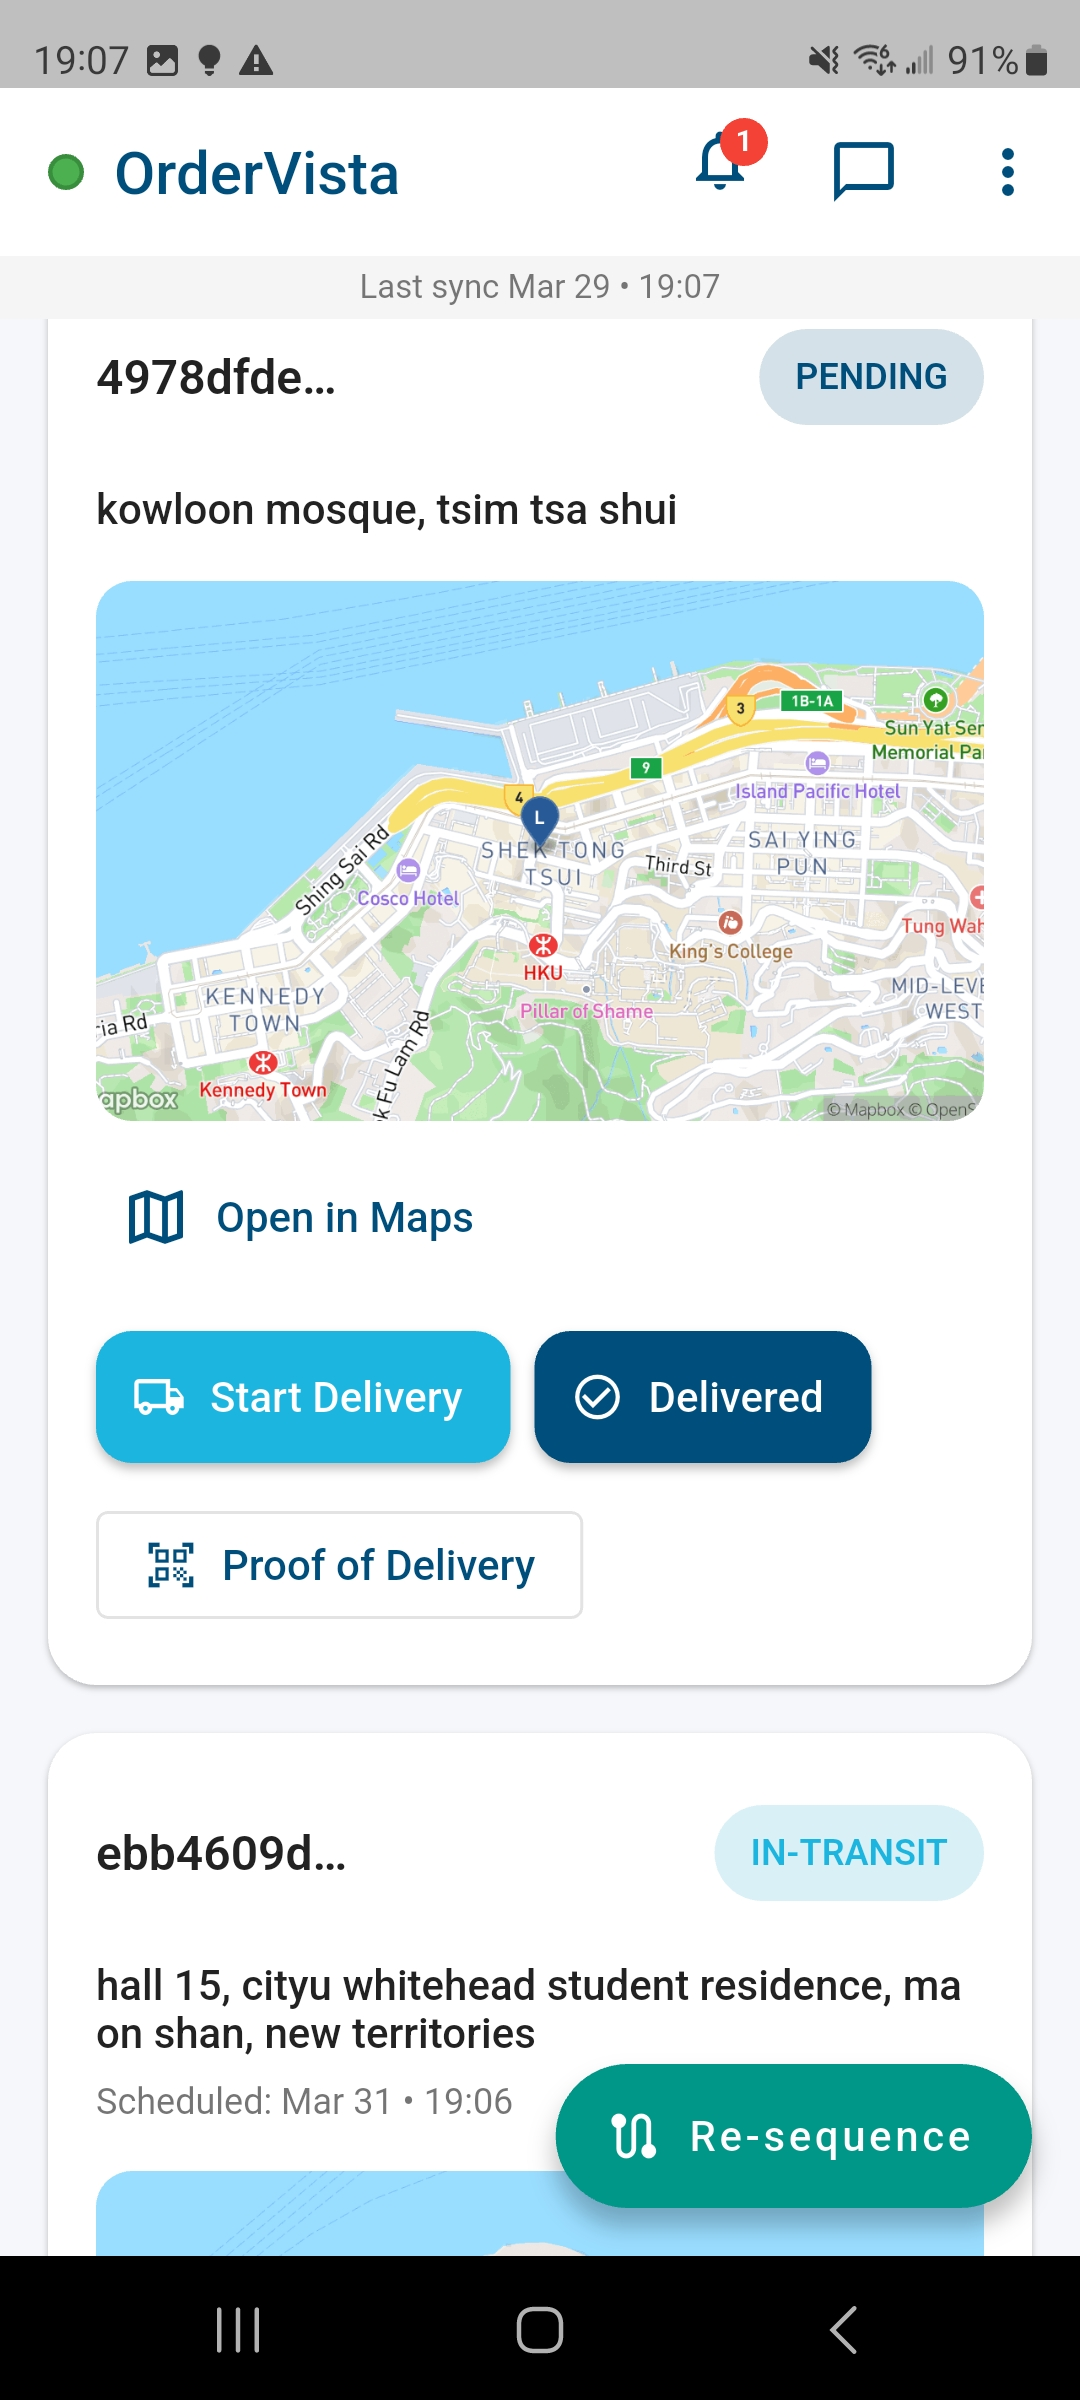
\includegraphics[width=0.45\textwidth]{ss-d3}
  \caption{Task marked as in-transit (D3).}
  \label{fig:ss-d3}
\end{figure}

\begin{figure}[H]
  \centering
  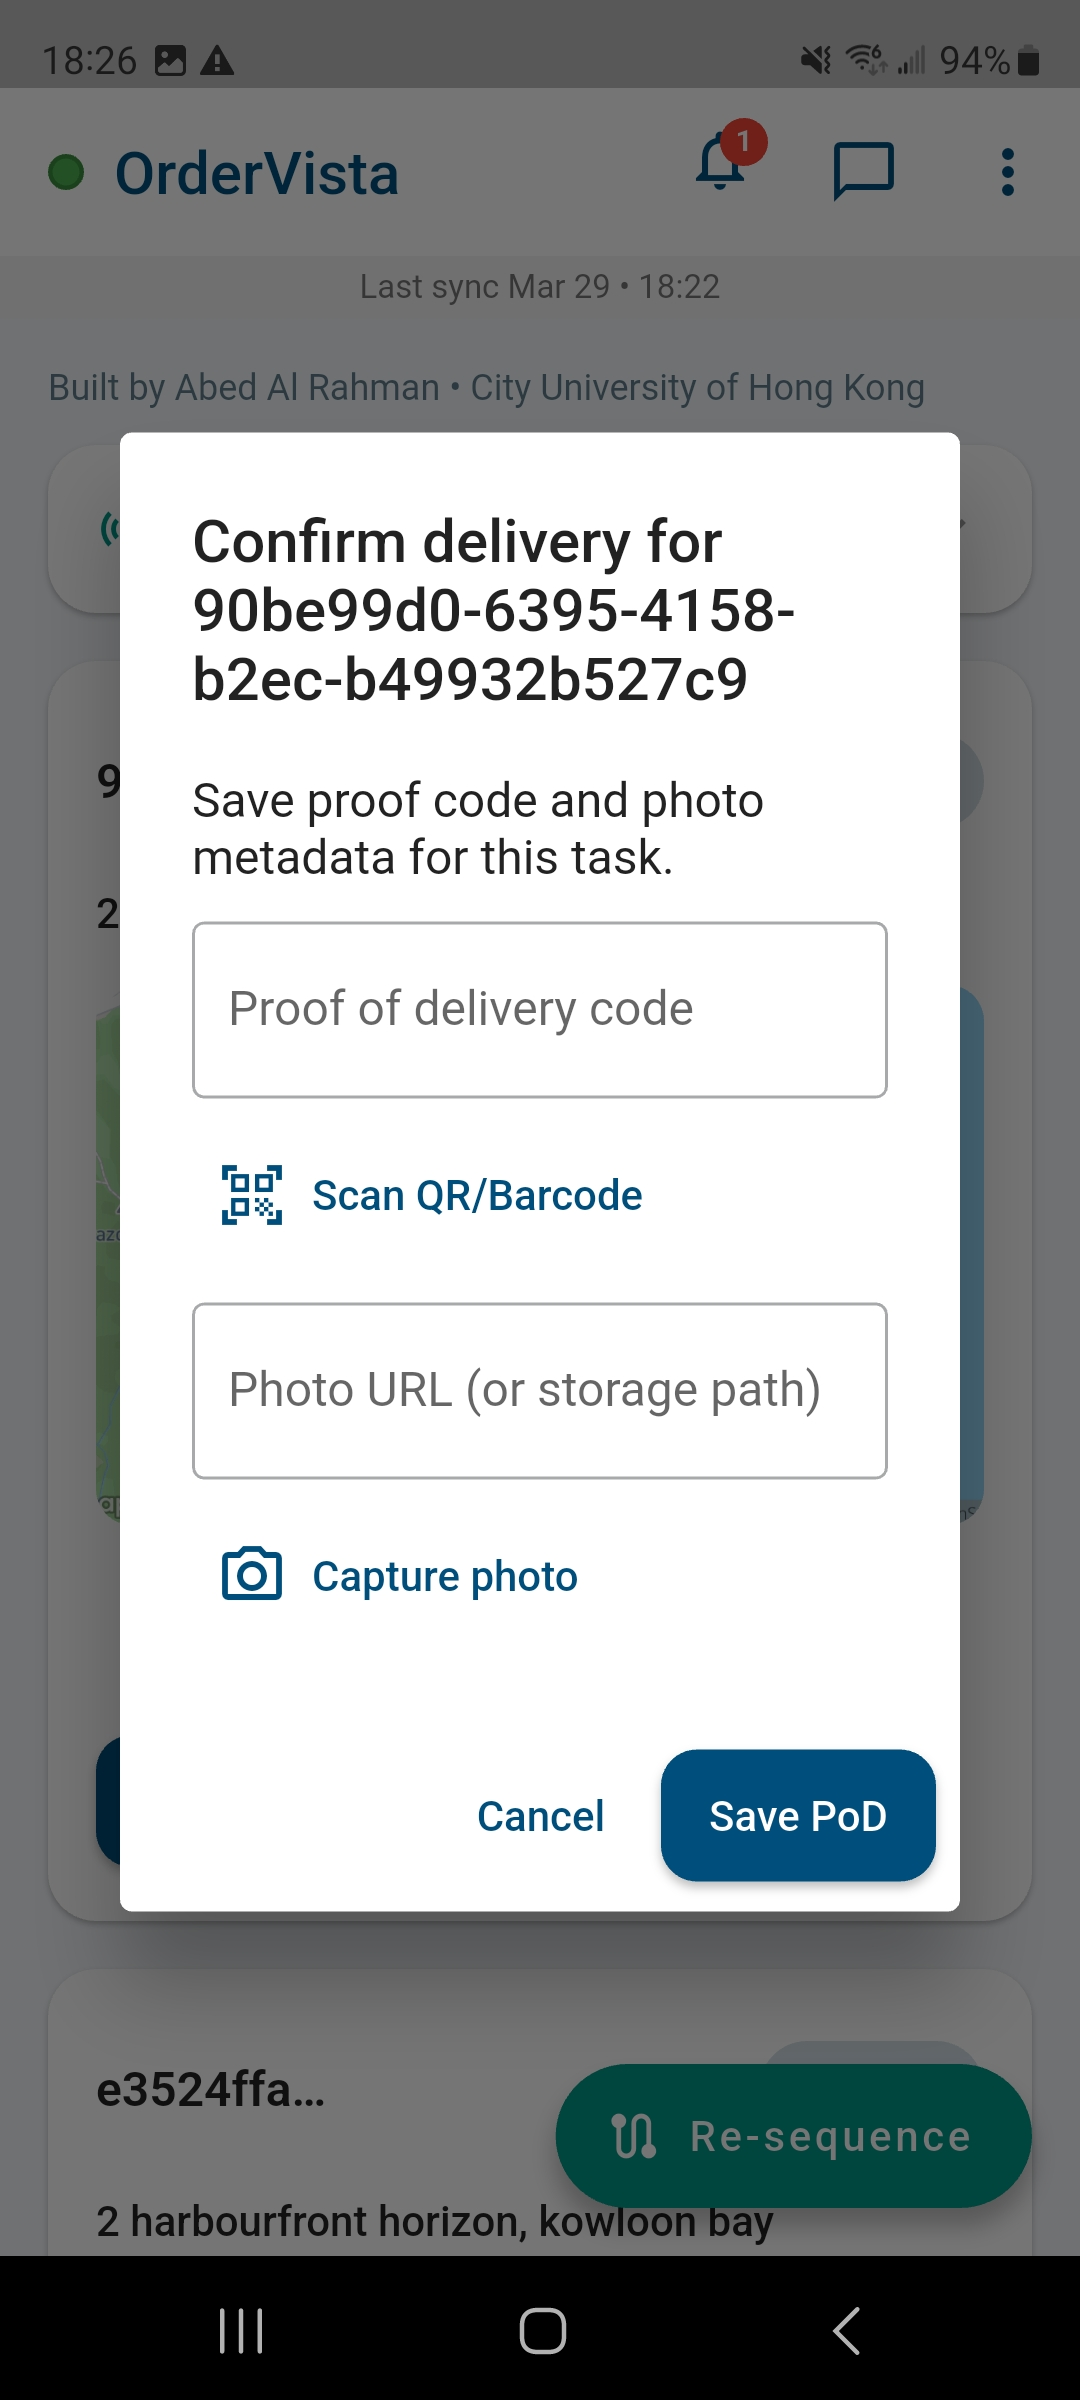
\includegraphics[width=0.45\textwidth]{ss-d4}
  \caption{Proof-of-delivery photo capture (D4).}
  \label{fig:ss-d4}
\end{figure}

\begin{figure}[H]
  \centering
  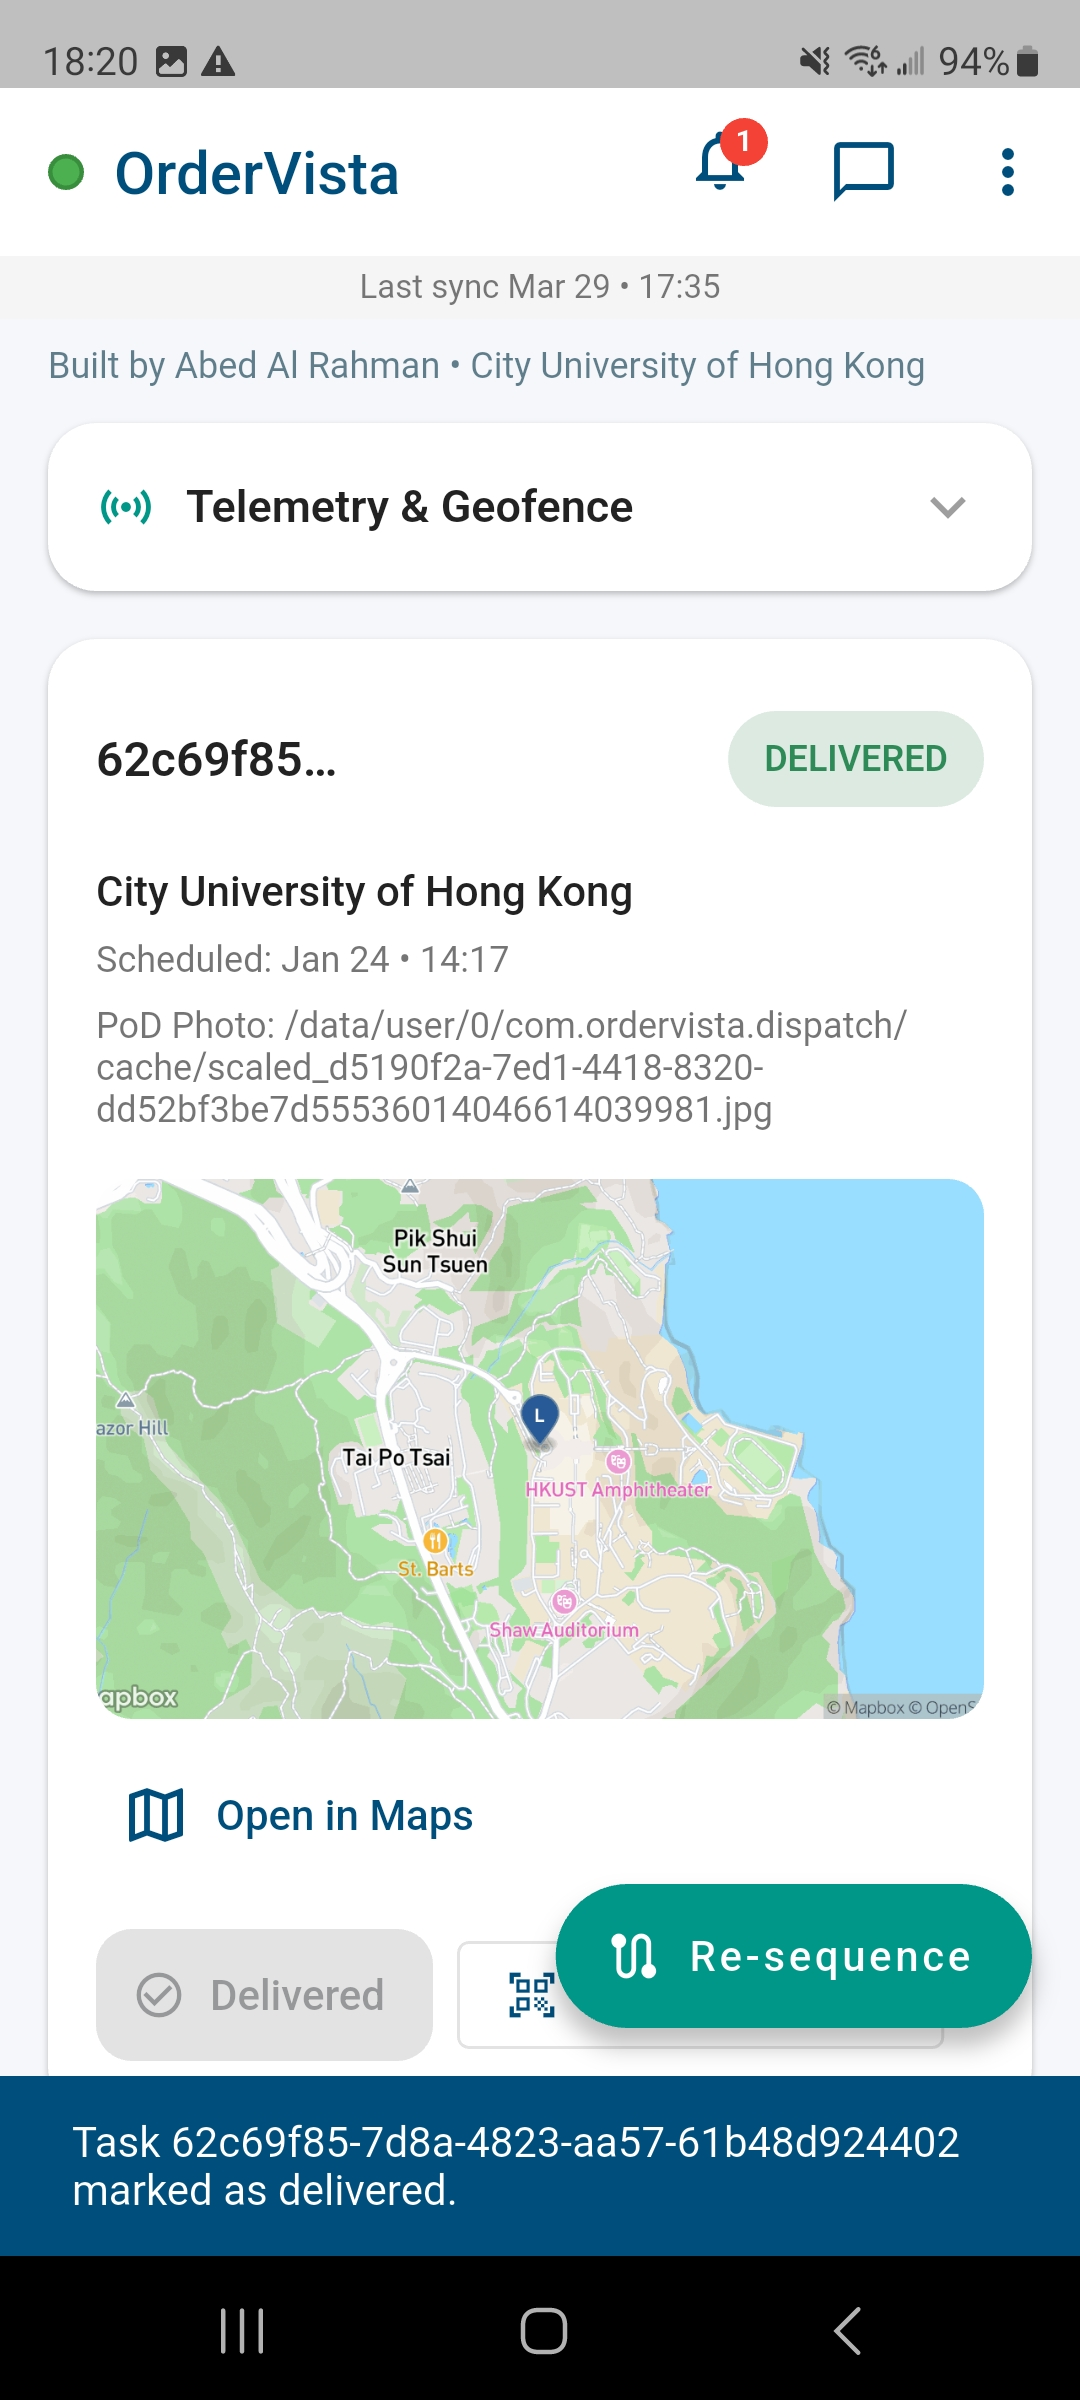
\includegraphics[width=0.45\textwidth]{ss-d5}
  \caption{Task marked as delivered with PoD confirmation (D5).}
  \label{fig:ss-d5}
\end{figure}

\begin{figure}[H]
  \centering
  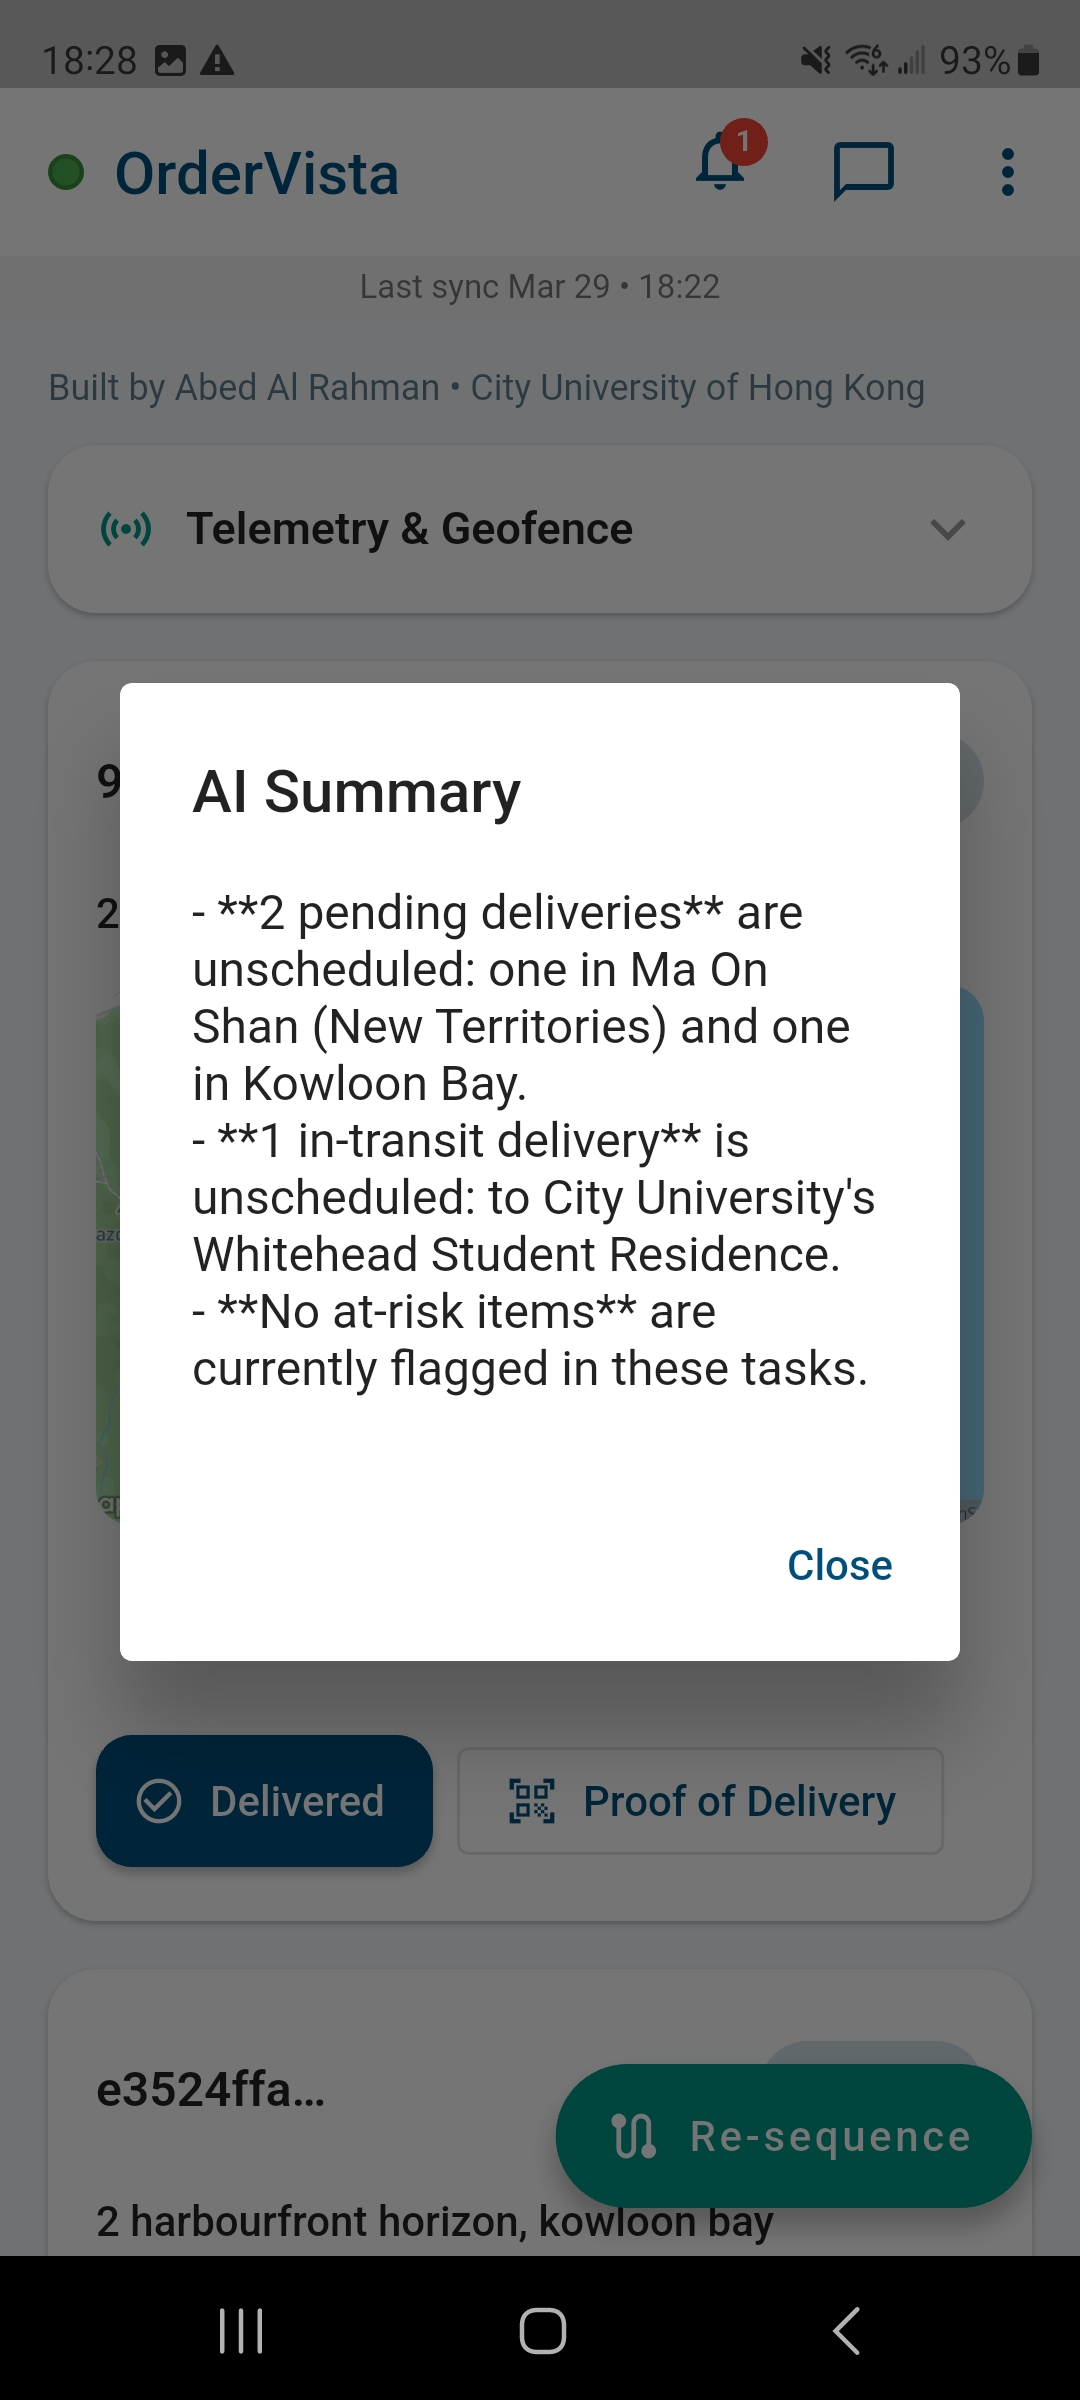
\includegraphics[width=0.45\textwidth]{ss-d6}
  \caption{AI task summary on driver device (D6).}
  \label{fig:ss-d6}
\end{figure}

\begin{figure}[H]
  \centering
  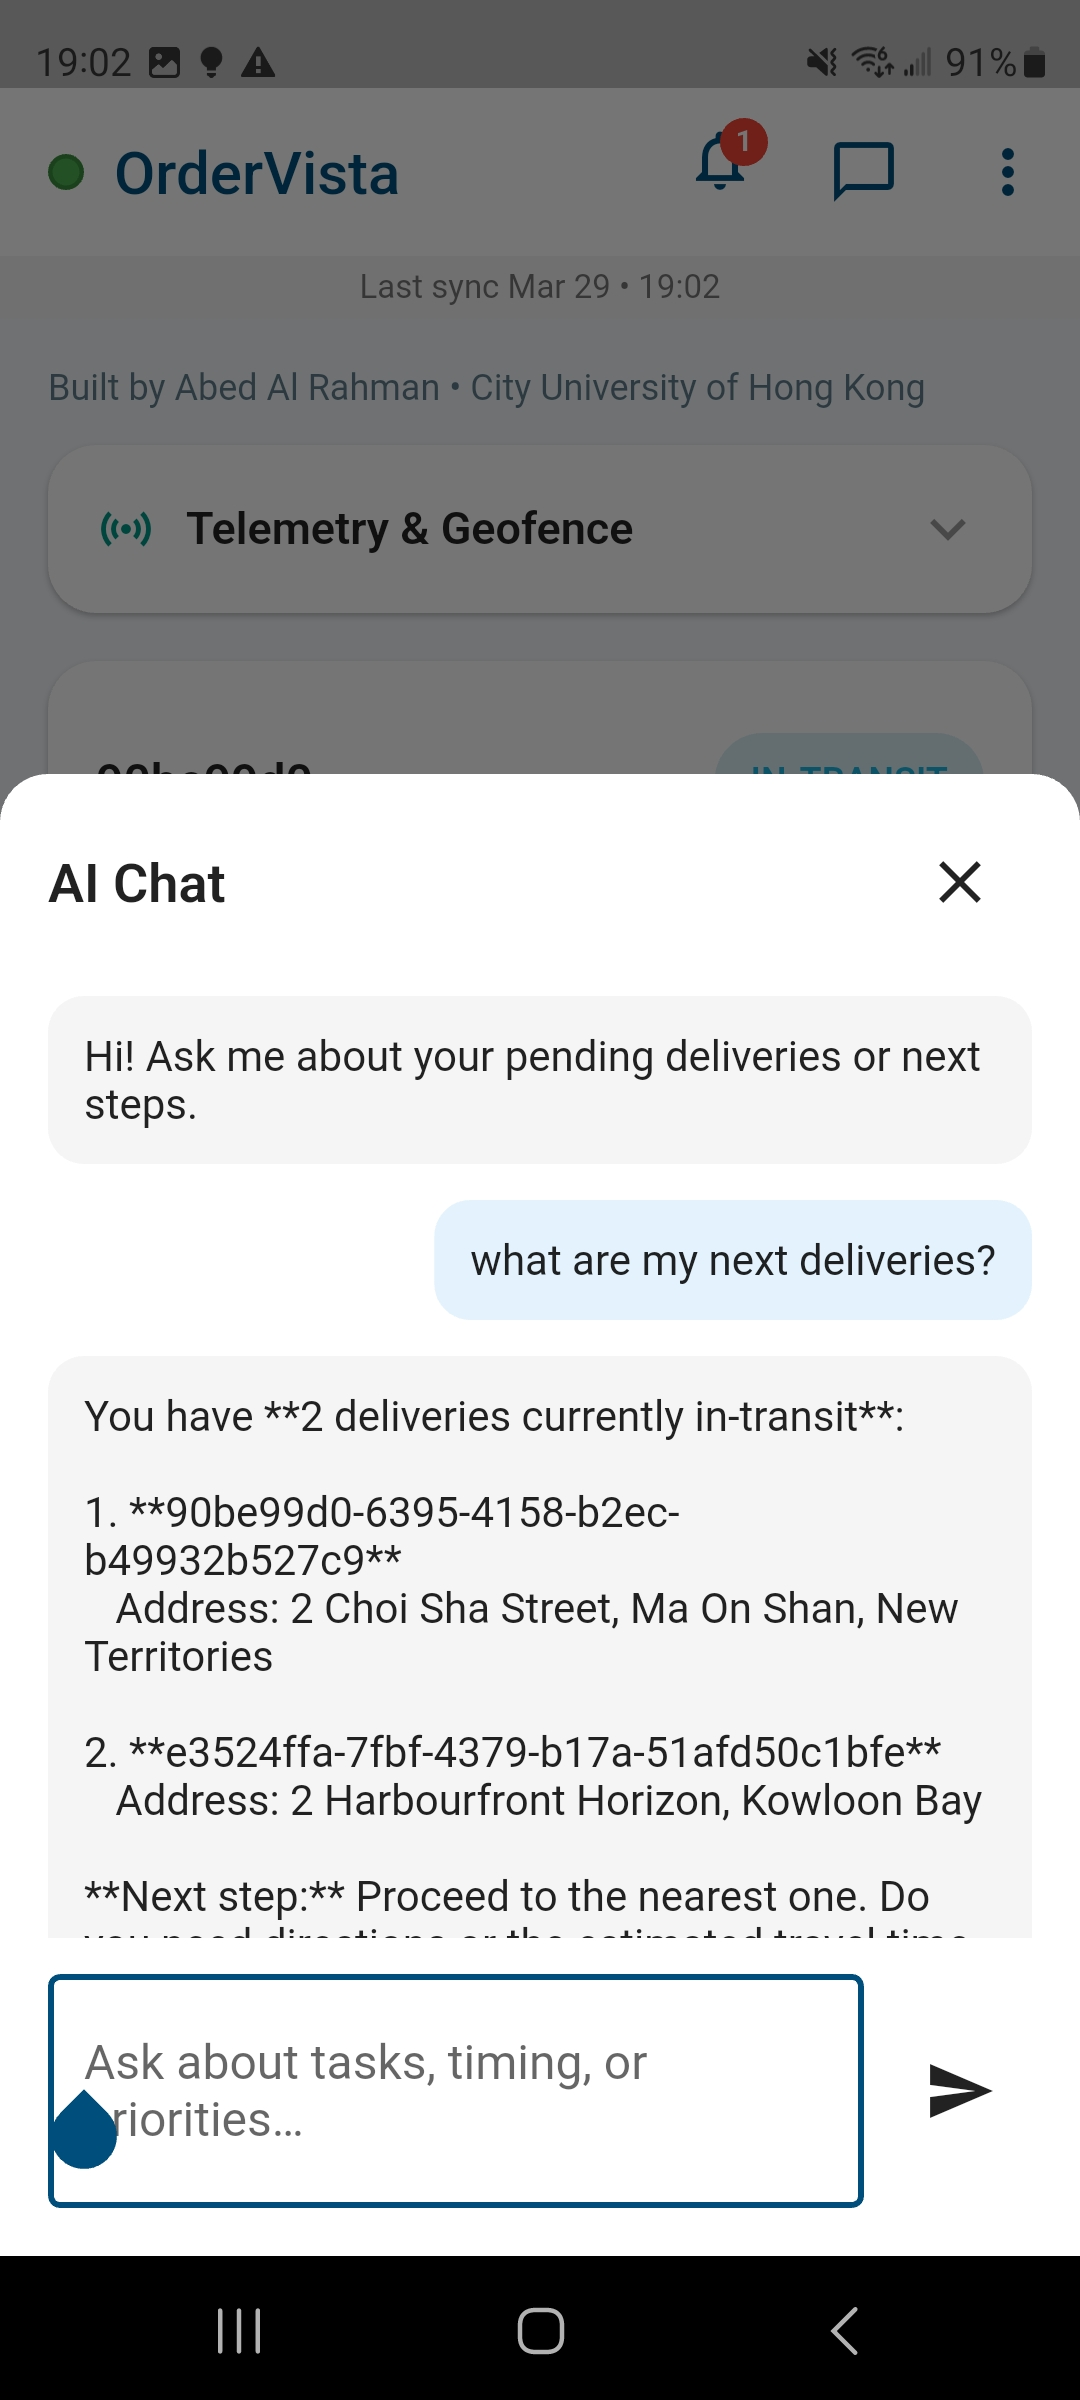
\includegraphics[width=0.45\textwidth]{ss-d7}
  \caption{AI free-form chat conversation (D7).}
  \label{fig:ss-d7}
\end{figure}

\begin{figure}[H]
  \centering
  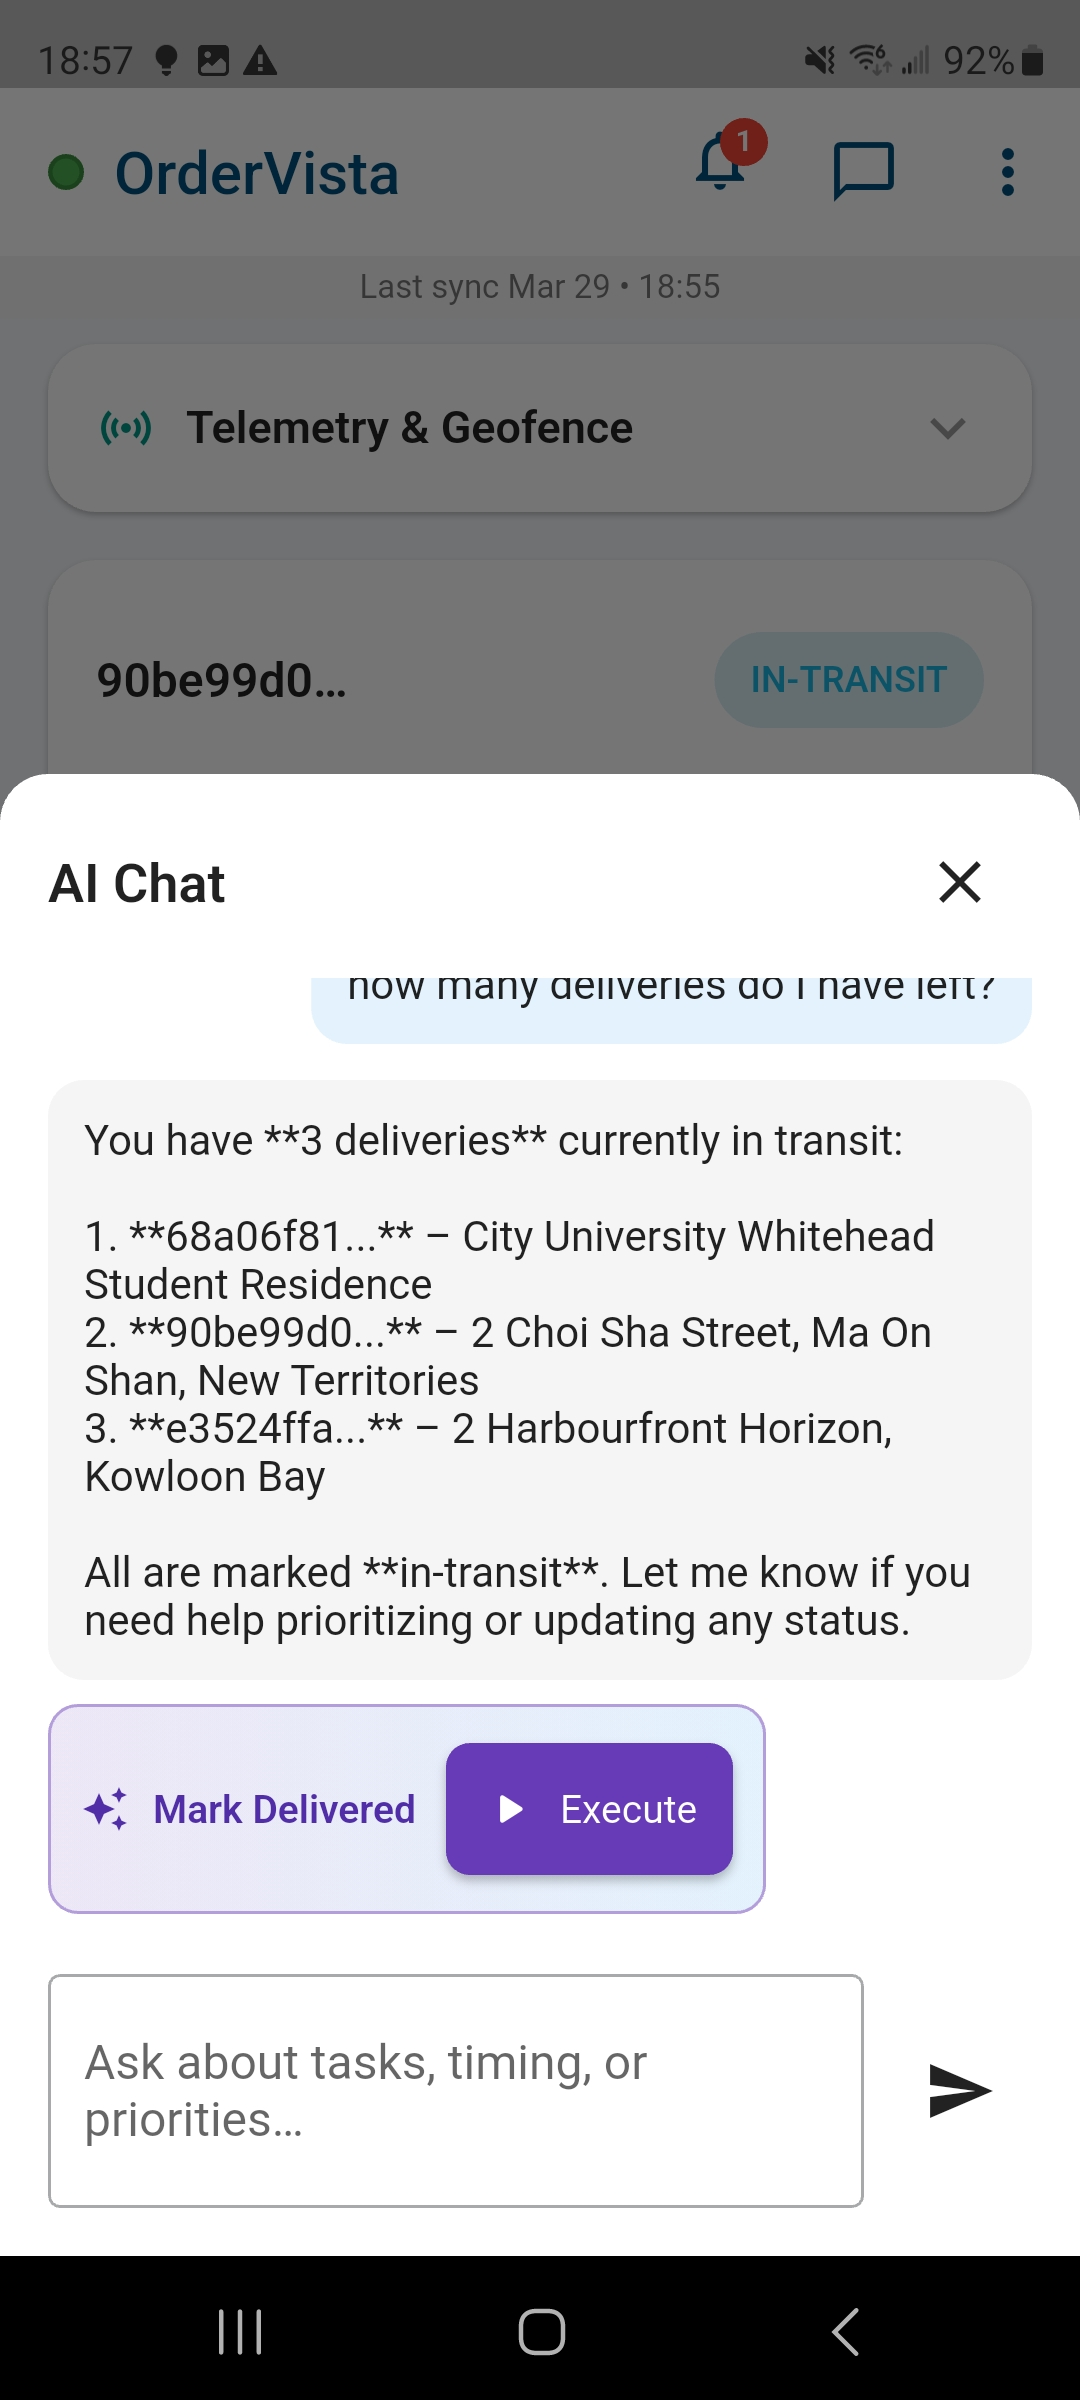
\includegraphics[width=0.45\textwidth]{ss-d8}
  \caption{Agentic AI suggestion with action chip (D8).}
  \label{fig:ss-d8}
\end{figure}

\begin{figure}[H]
  \centering
  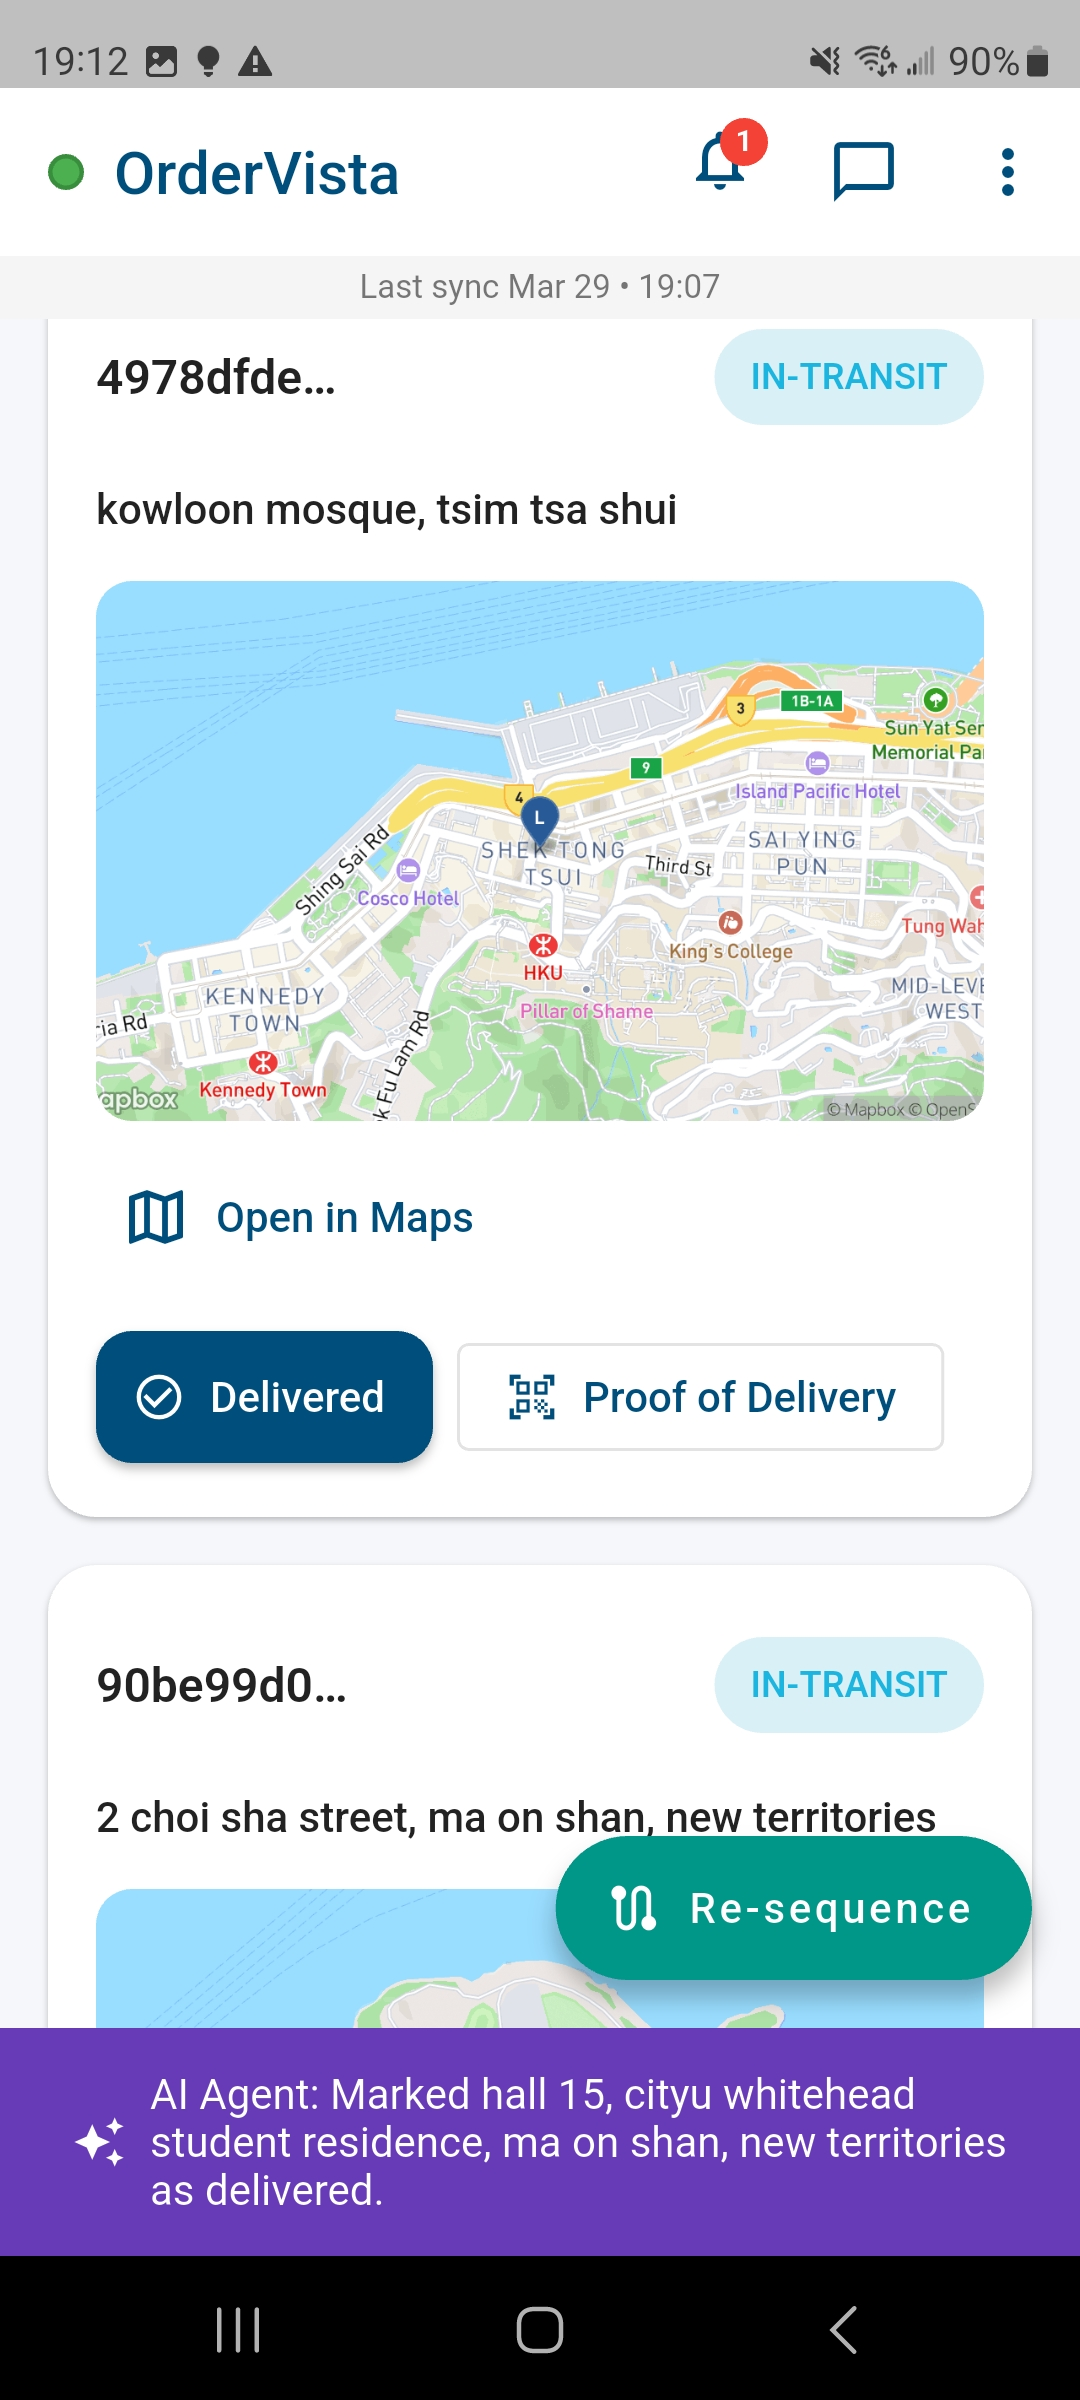
\includegraphics[width=0.45\textwidth]{ss-d9}
  \caption{Agentic action executed after user confirmation (D9).}
  \label{fig:ss-d9}
\end{figure}

\begin{figure}[H]
  \centering
  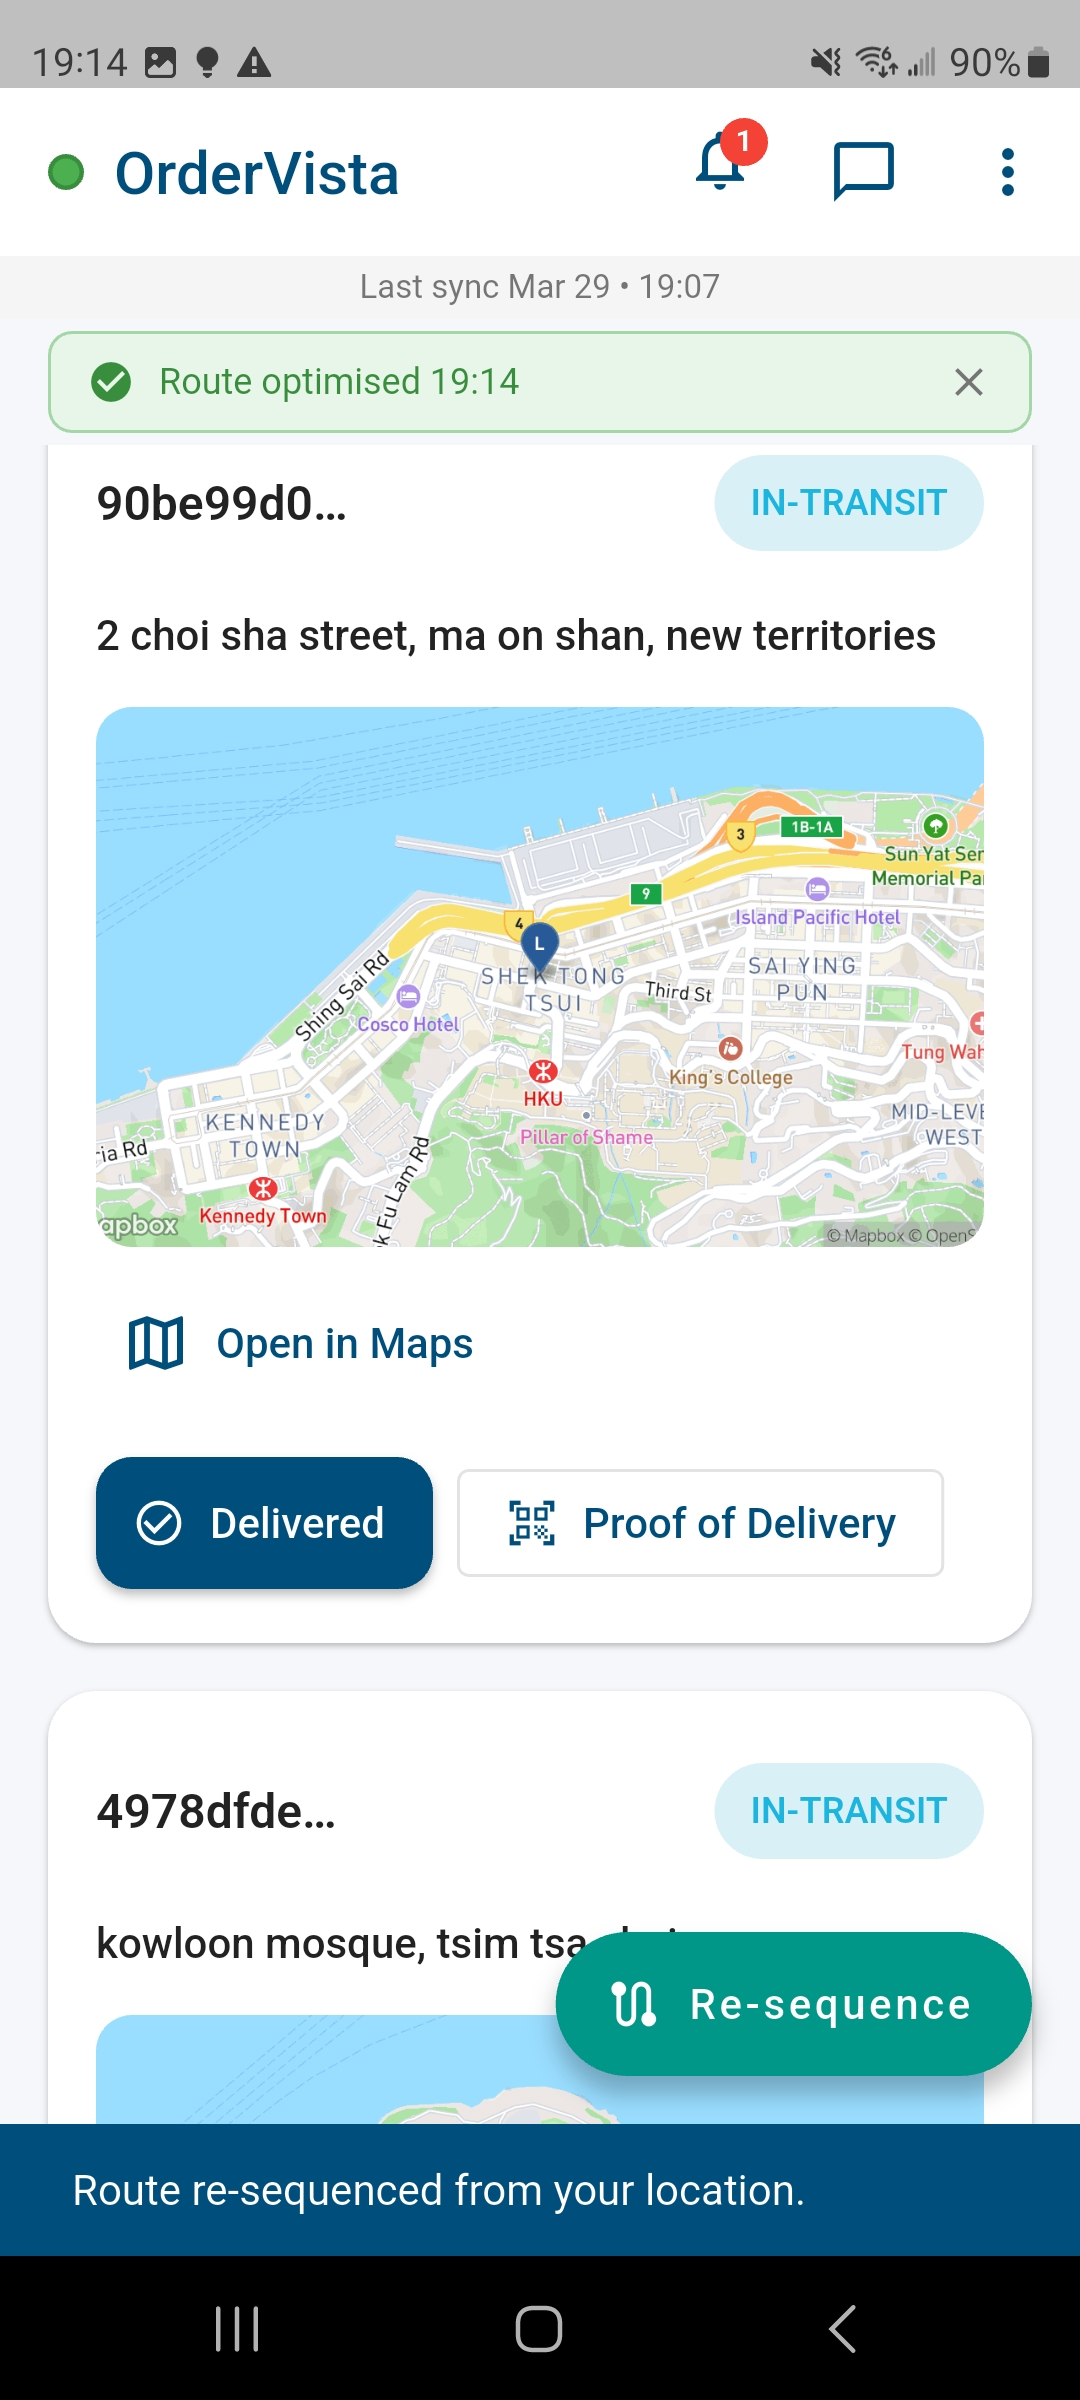
\includegraphics[width=0.45\textwidth]{ss-d10}
  \caption{Task list after mid-shift GPS re-sequencing (D10).}
  \label{fig:ss-d10}
\end{figure}

\begin{figure}[H]
  \centering
  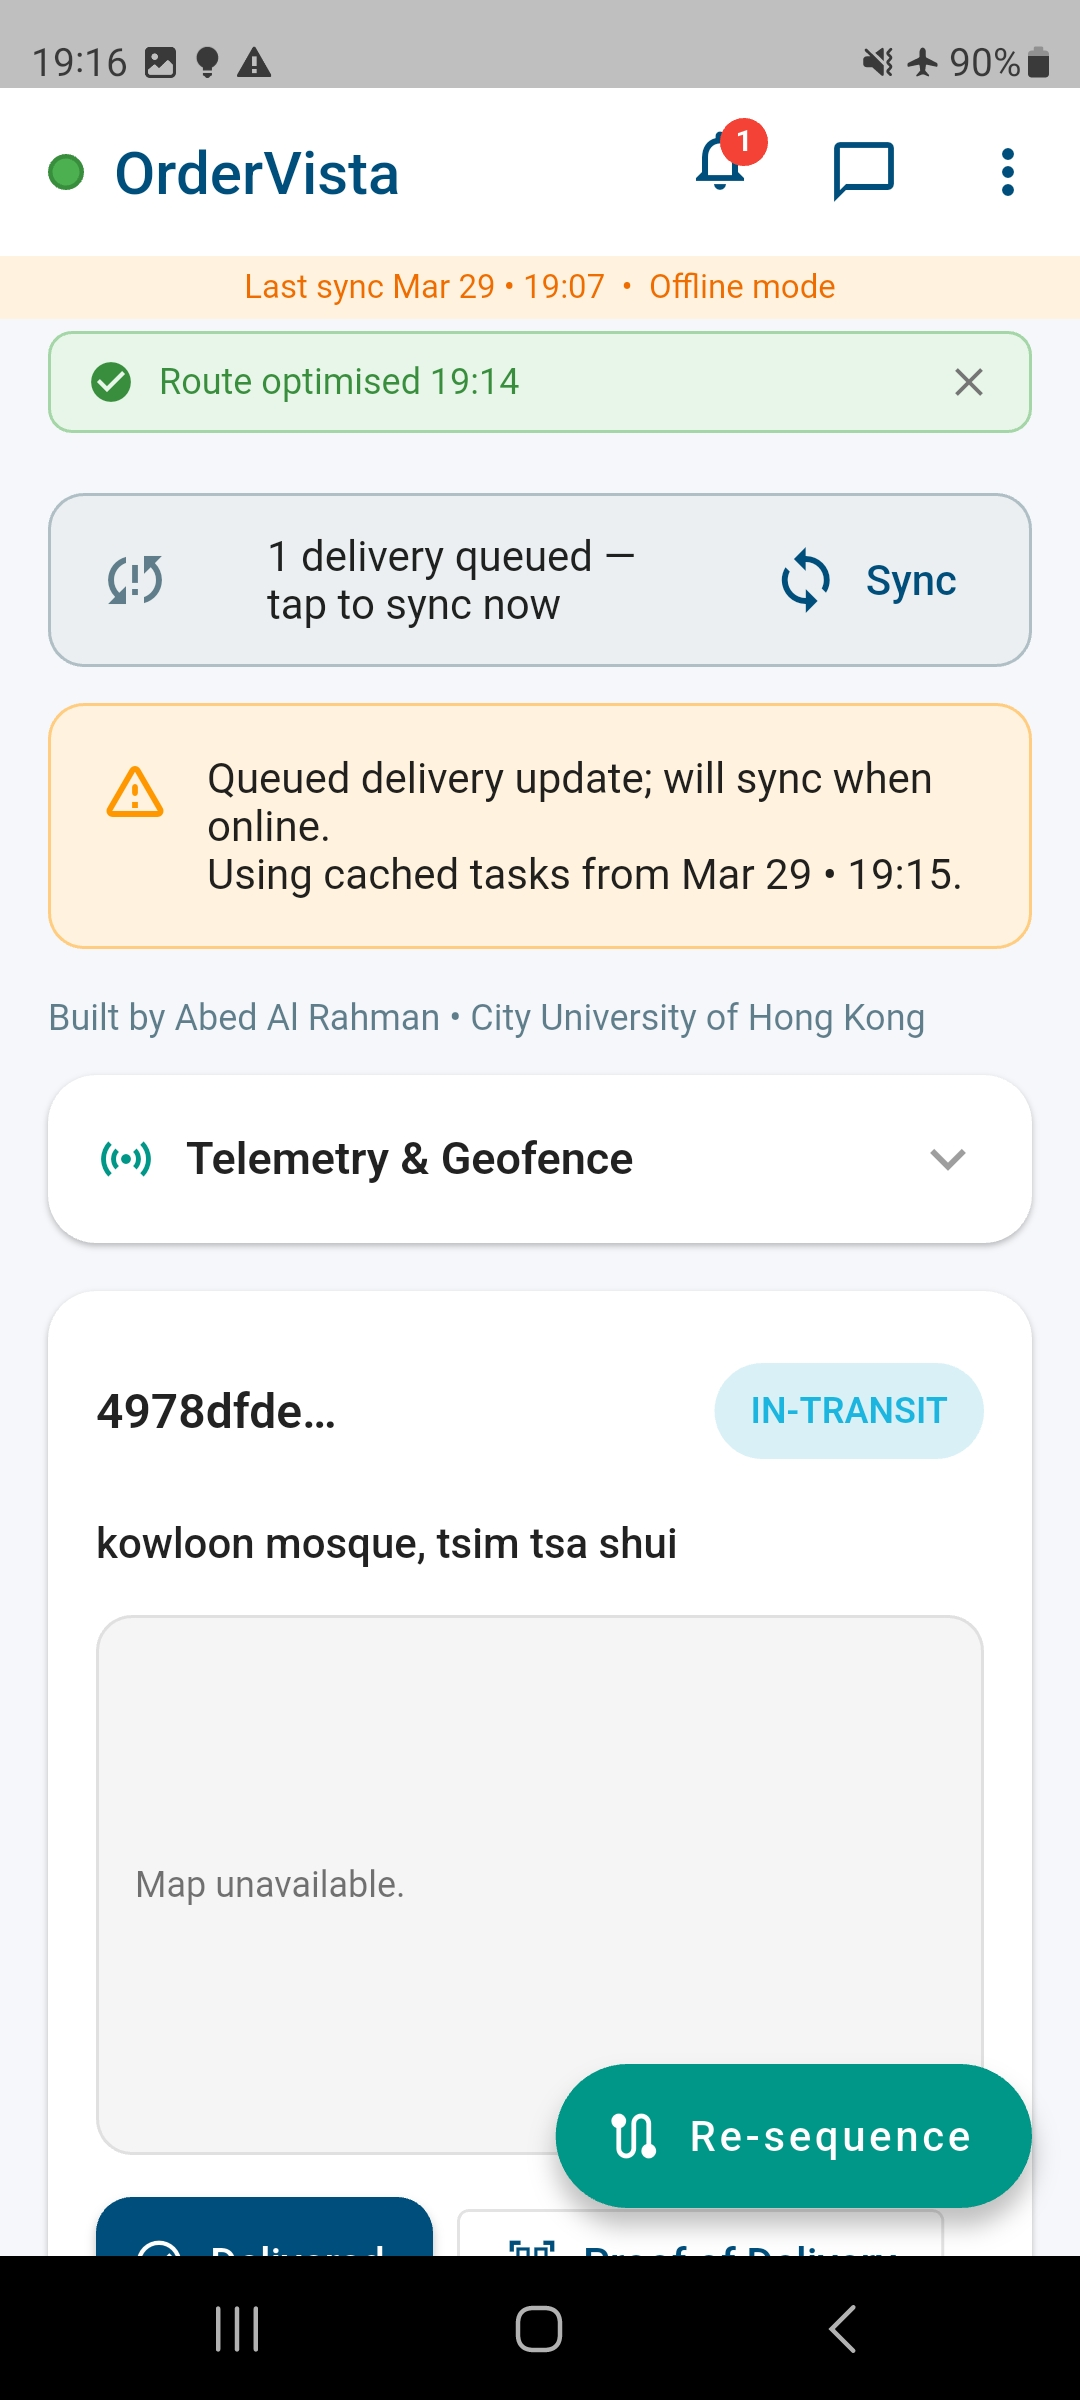
\includegraphics[width=0.45\textwidth]{ss-d11}
  \caption{Offline delivery queued and synced on reconnect (D11).}
  \label{fig:ss-d11}
\end{figure}

\begin{figure}[H]
  \centering
  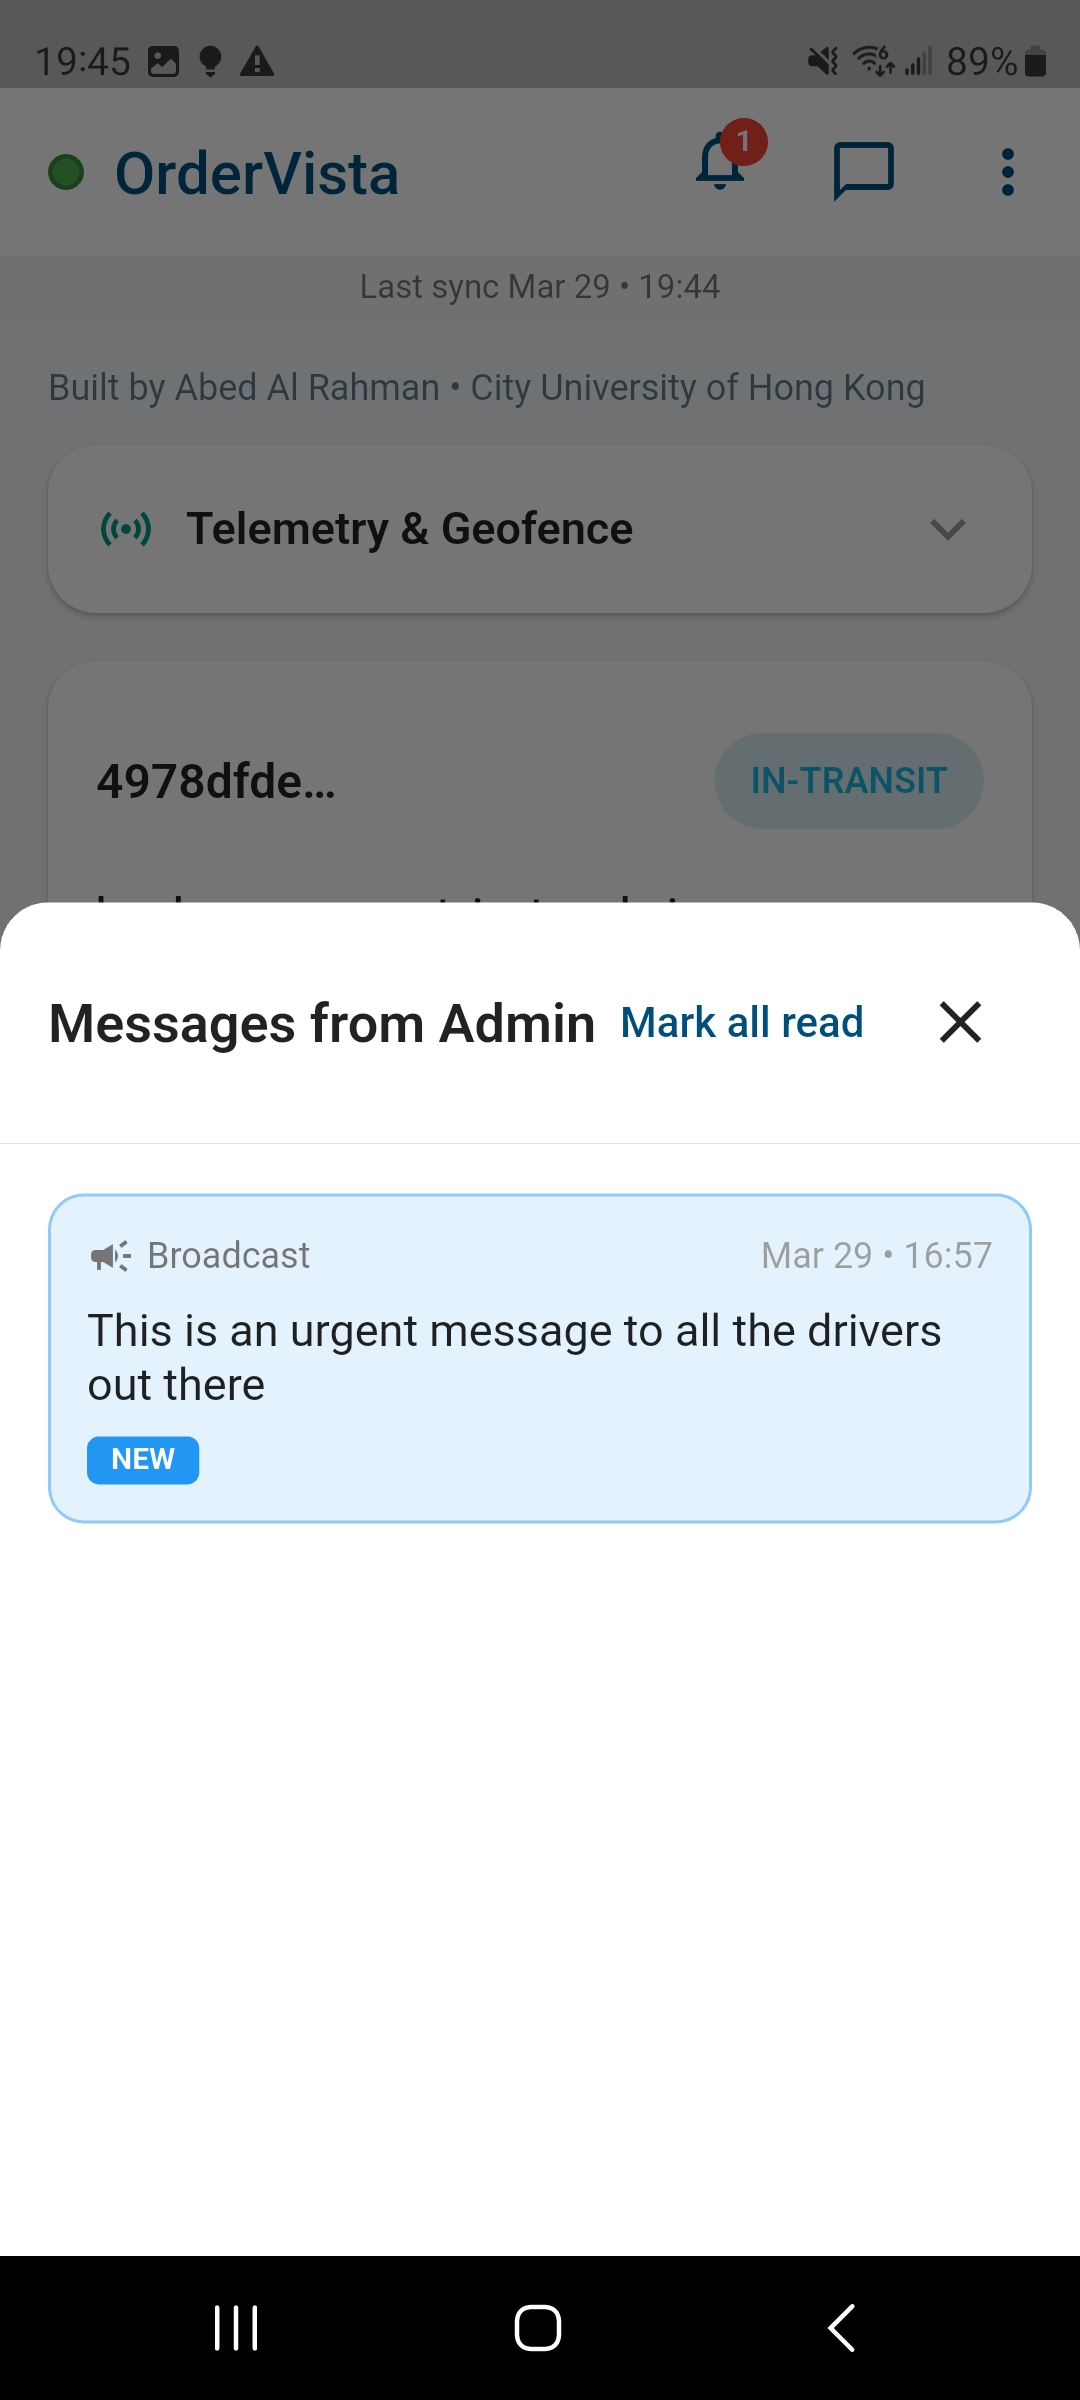
\includegraphics[width=0.45\textwidth]{ss-d12}
  \caption{Chat message received from admin (D12).}
  \label{fig:ss-d12}
\end{figure}

\begin{figure}[H]
  \centering
  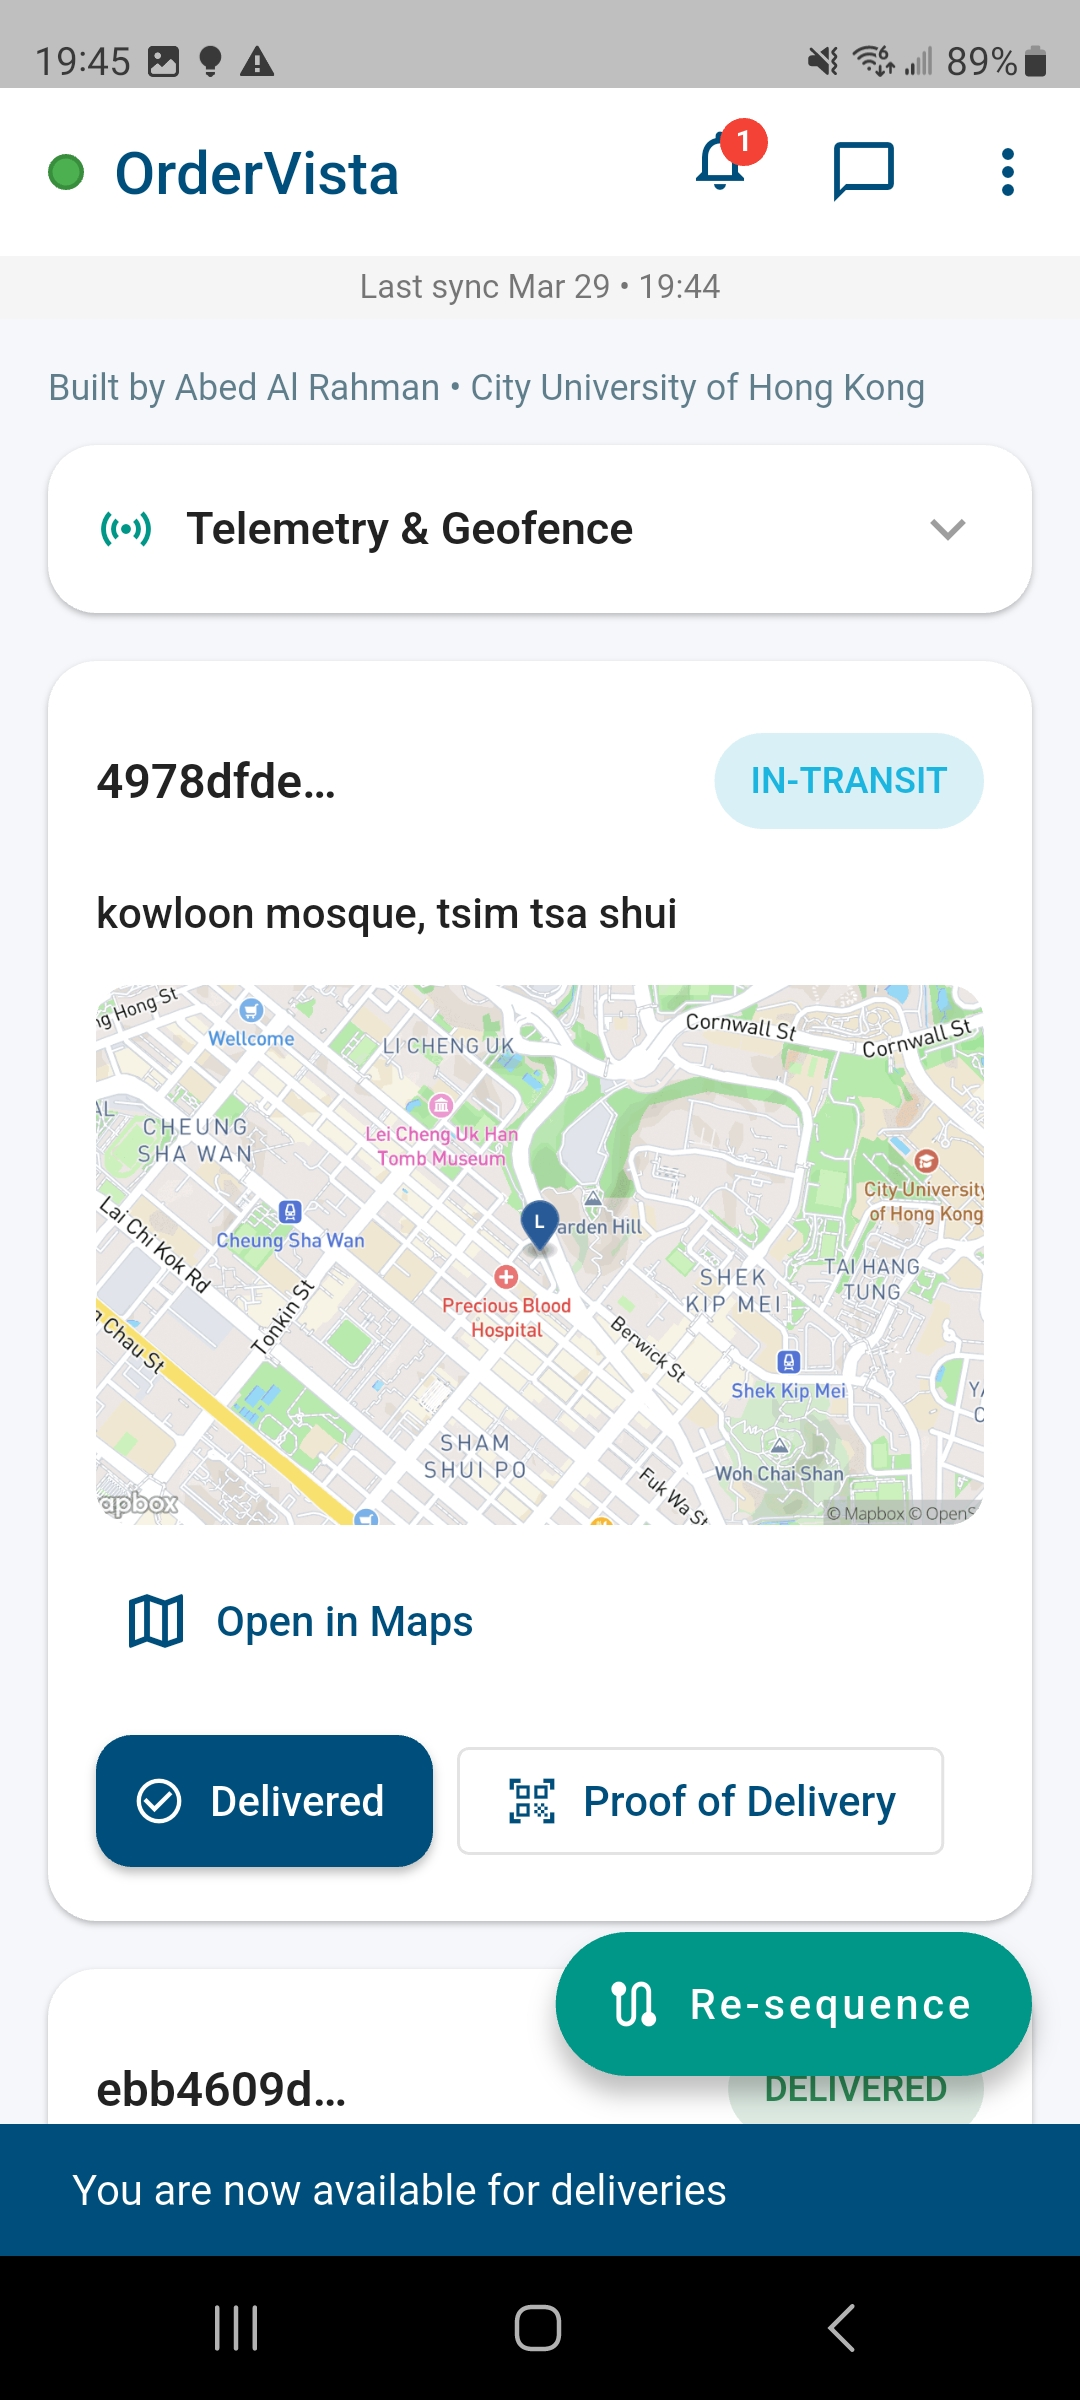
\includegraphics[width=0.45\textwidth]{ss-d13}
  \caption{Driver availability toggle (D13).}
  \label{fig:ss-d13}
\end{figure}

\begin{figure}[H]
  \centering
  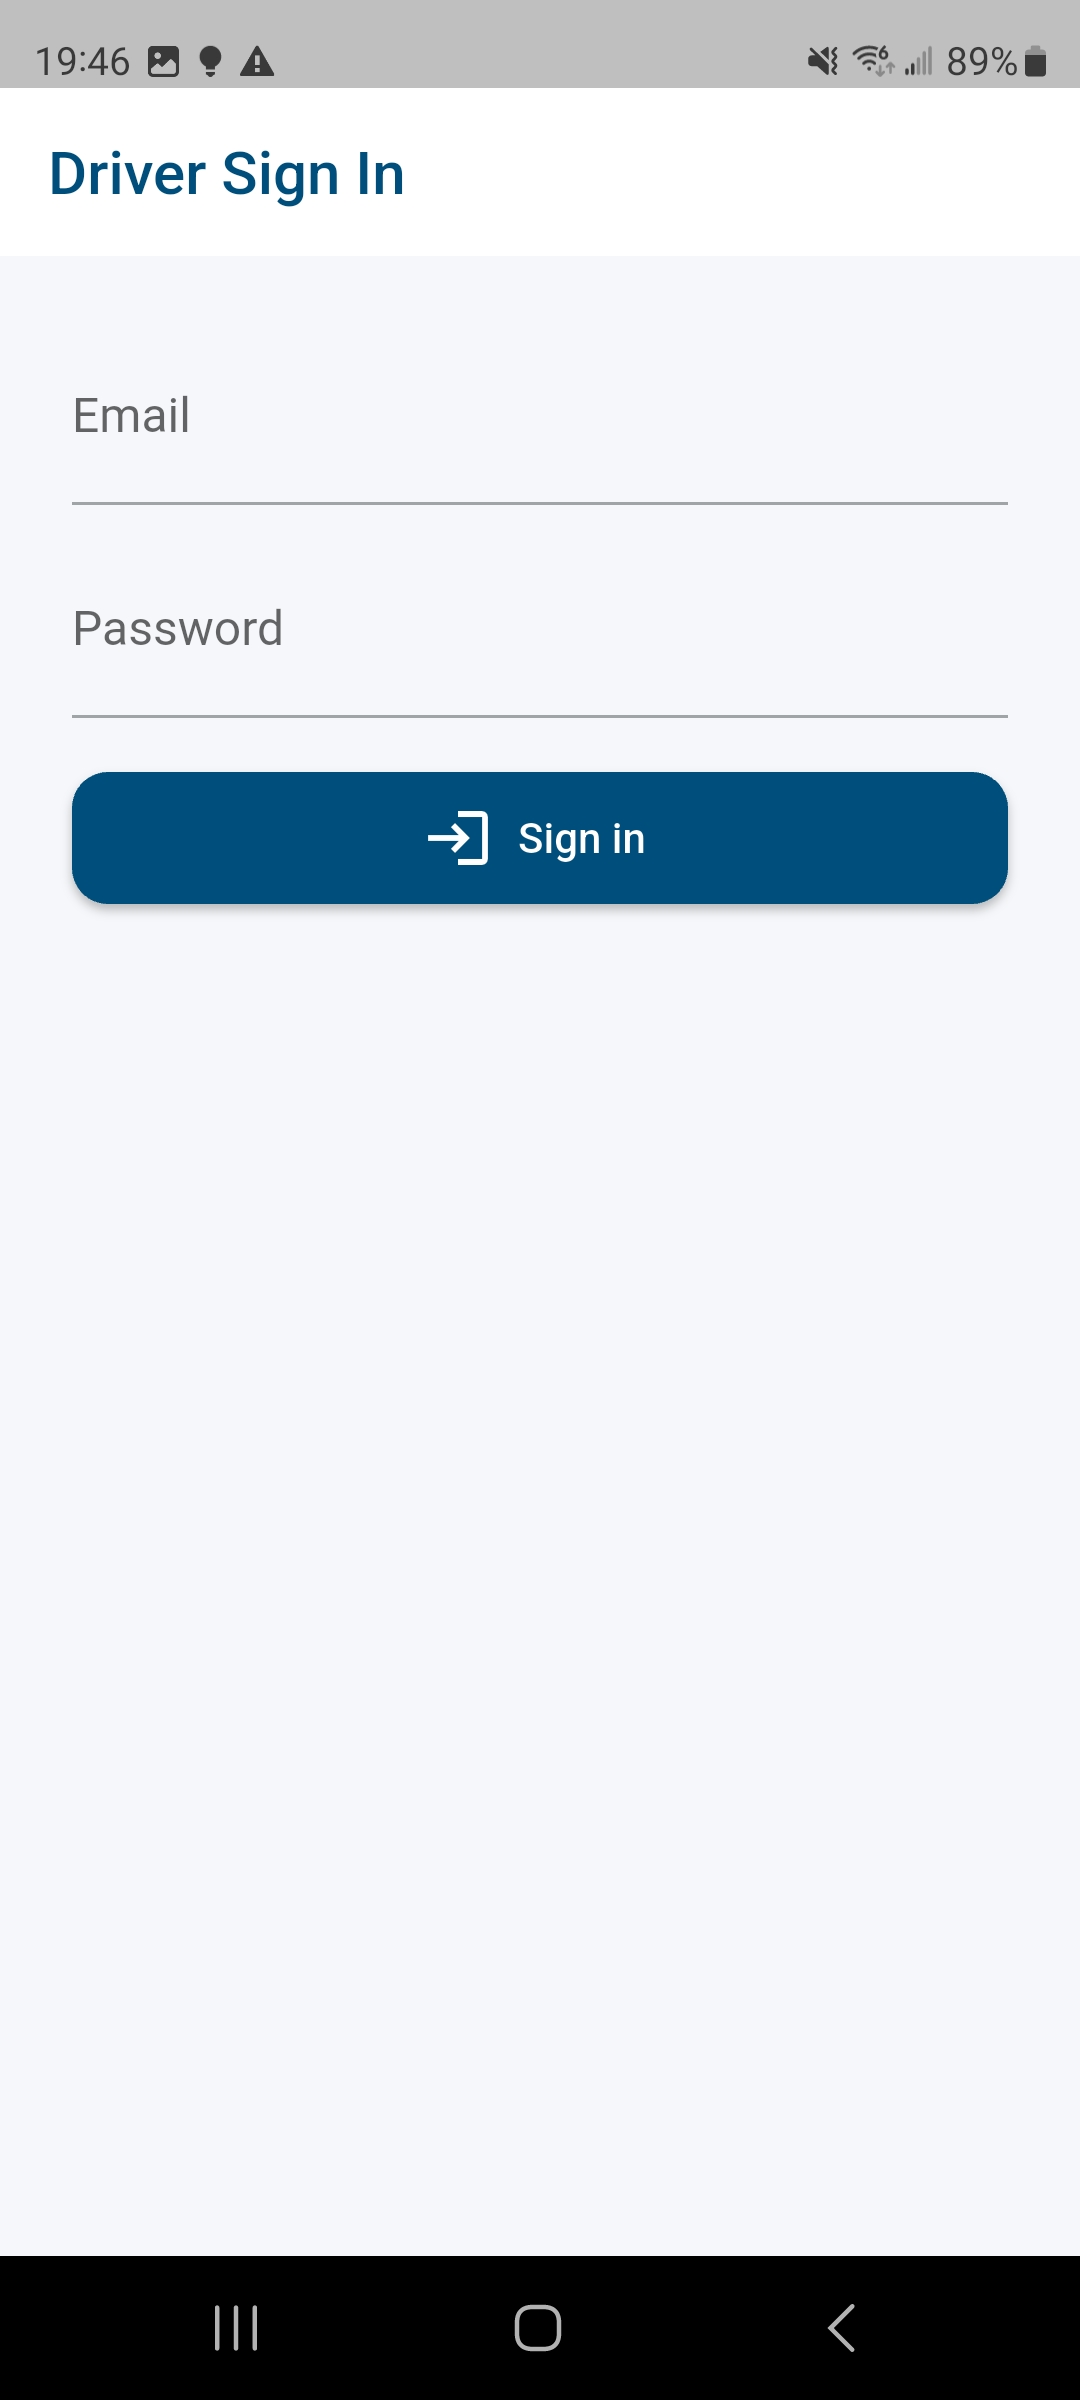
\includegraphics[width=0.45\textwidth]{ss-d14}
  \caption{Sign-out returning to login screen (D14).}
  \label{fig:ss-d14}
\end{figure}

\clearpage
% ─────────────────────────────────────────────────────────────
\section{Security Verification}
\label{sec:security-test}

\subsection{RLS Cross-Tenant Isolation}
\label{sec:rls-test}

To verify that Row-Level Security prevents cross-tenant data leakage, the
following test was performed:

\begin{enumerate}
  \item Two test companies were created (\emph{Company~A} and
        \emph{Company~B}), each with an admin user and sample tasks.
  \item Logged in as Company~A's admin.
  \item Executed a direct PostgREST query for Company~B's tasks:
\end{enumerate}

\begin{lstlisting}[language=SQL, caption={Cross-tenant query (expected: 0 rows).}, label={lst:rls-test}]
-- Authenticated as Company A user via Supabase JWT
SELECT * FROM tasks
WHERE company_id = '<company_b_uuid>';
-- Result: 0 rows returned (RLS blocked)
\end{lstlisting}

The query returned zero rows, confirming that the \texttt{is\_company\_member()}
RLS helper function correctly blocks cross-tenant reads.  The same test was
repeated for the \texttt{routes}, \texttt{route\_tasks},
\texttt{telemetry\_events}, and \texttt{chat\_messages} tables, all of which returned
zero rows when queried from the wrong tenant context.

\begin{figure}[H]
  \centering
  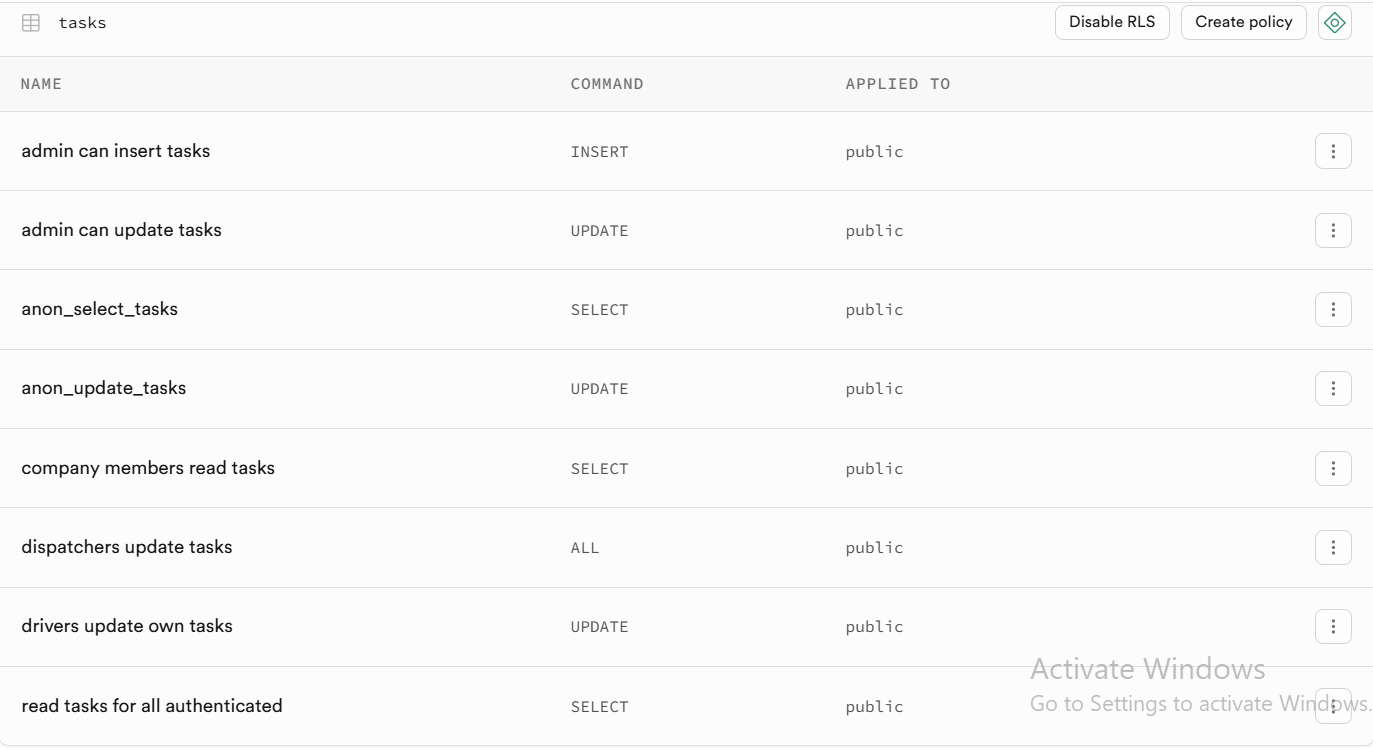
\includegraphics[width=0.7\textwidth]{Task_Policies_Supabase}
  \caption{RLS policies on the \texttt{tasks} table enforcing cross-tenant isolation.}
  \label{fig:ss-rls}
\end{figure}

\subsection{RBAC Enforcement}
\label{sec:rbac-test}

Table~\ref{tab:rbac-test} summarises the RBAC tests.

\begin{table}[H]
  \centering
  \caption{RBAC enforcement test results.}
  \label{tab:rbac-test}
  \small
  \begin{tabularx}{\textwidth}{X l l}
    \toprule
    \textbf{Action attempted} & \textbf{As driver} & \textbf{As admin} \\
    \midrule
    Create a new task              & Blocked (403) & Allowed \\
    Delete a task                  & Blocked (403) & Allowed \\
    Generate a route               & Blocked (403) & Allowed \\
    Update own task status         & Allowed       & Allowed \\
    Upload PoD photo               & Allowed       & Allowed \\
    View other company's tasks     & 0 rows (RLS)  & 0 rows (RLS) \\
    Send chat message              & Allowed       & Allowed \\
    Read another driver's chat     & 0 rows (RLS)  & 0 rows (RLS) \\
    \bottomrule
  \end{tabularx}
\end{table}

% ─────────────────────────────────────────────────────────────
\section{Route Optimisation Evaluation}
\label{sec:route-eval}

To evaluate whether the nearest-neighbour heuristic produces meaningful
distance reductions, the same set of Hong Kong delivery addresses was
sequenced using the unoptimised input order (baseline) and the OrderVista
nearest-neighbour algorithm.  Three batch sizes ($n \in \{5, 10, 15\}$) were
tested, representative of typical dispatcher workloads.

\begin{table}[H]
  \centering
  \caption{Route optimisation: distance and time-proxy improvement versus
           unoptimised baseline.}
  \label{tab:route-eval}
  \small
  \begin{tabular}{r r r r r r r}
    \toprule
    & \multicolumn{3}{c}{\textbf{Distance (km)}} &
      \multicolumn{3}{c}{\textbf{Time proxy (min)}} \\
    \cmidrule(lr){2-4} \cmidrule(lr){5-7}
    $n$ & Baseline & OrderVista & $\Delta$ &
          Baseline & OrderVista & $\Delta$ \\
    \midrule
     5  & 18.4 & 12.7 & $-31.0\%$ & 55  & 41  & $-25.5\%$ \\
    10  & 34.6 & 25.8 & $-25.4\%$ & 104 & 80  & $-23.1\%$ \\
    15  & 49.8 & 36.9 & $-25.9\%$ & 149 & 114 & $-23.5\%$ \\
    \bottomrule
  \end{tabular}
\end{table}

The nearest-neighbour heuristic reduces total route distance by
\textbf{25--31\%} across all batch sizes (Table~\ref{tab:route-eval}).  The
time-proxy column represents a proportional estimate (shorter distance implies
lower travel time under typical urban driving conditions).  While the heuristic
does not guarantee global optimality, the consistent improvement confirms that
OrderVista performs meaningful route optimisation rather than arbitrary
reordering \autocite{laporte2009fifty}.

\begin{figure}[H]
  \centering
  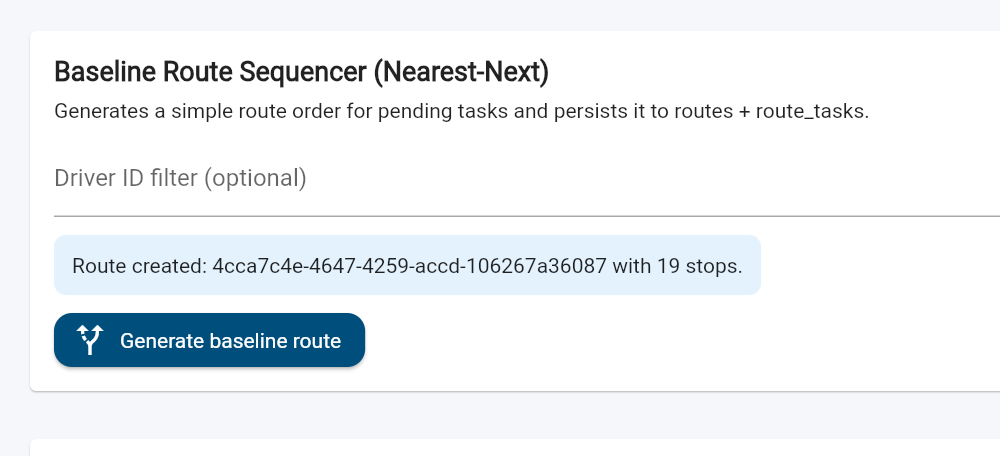
\includegraphics[width=0.7\textwidth]{ss-a6}
  \caption{Visual comparison of baseline vs.\ optimised route (optional).}
  \label{fig:ss-route-compare}
\end{figure}

% ─────────────────────────────────────────────────────────────
\section{AI Evaluation}
\label{sec:ai-eval}

\subsection{Task Summarisation Quality}
\label{sec:ai-summary-eval}

The AI summarisation feature was tested with five different task-list
configurations (varying counts of pending, in-transit, and delivered tasks).
In all five cases, the generated summary correctly:

\begin{itemize}
  \item reported the number of remaining deliveries,
  \item identified the next scheduled task,
  \item avoided fabricating task details not present in the input.
\end{itemize}

\noindent Temperature was set to $0.3$, and no hallucinations were observed
across the five test runs.

\begin{figure}[H]
  \centering
  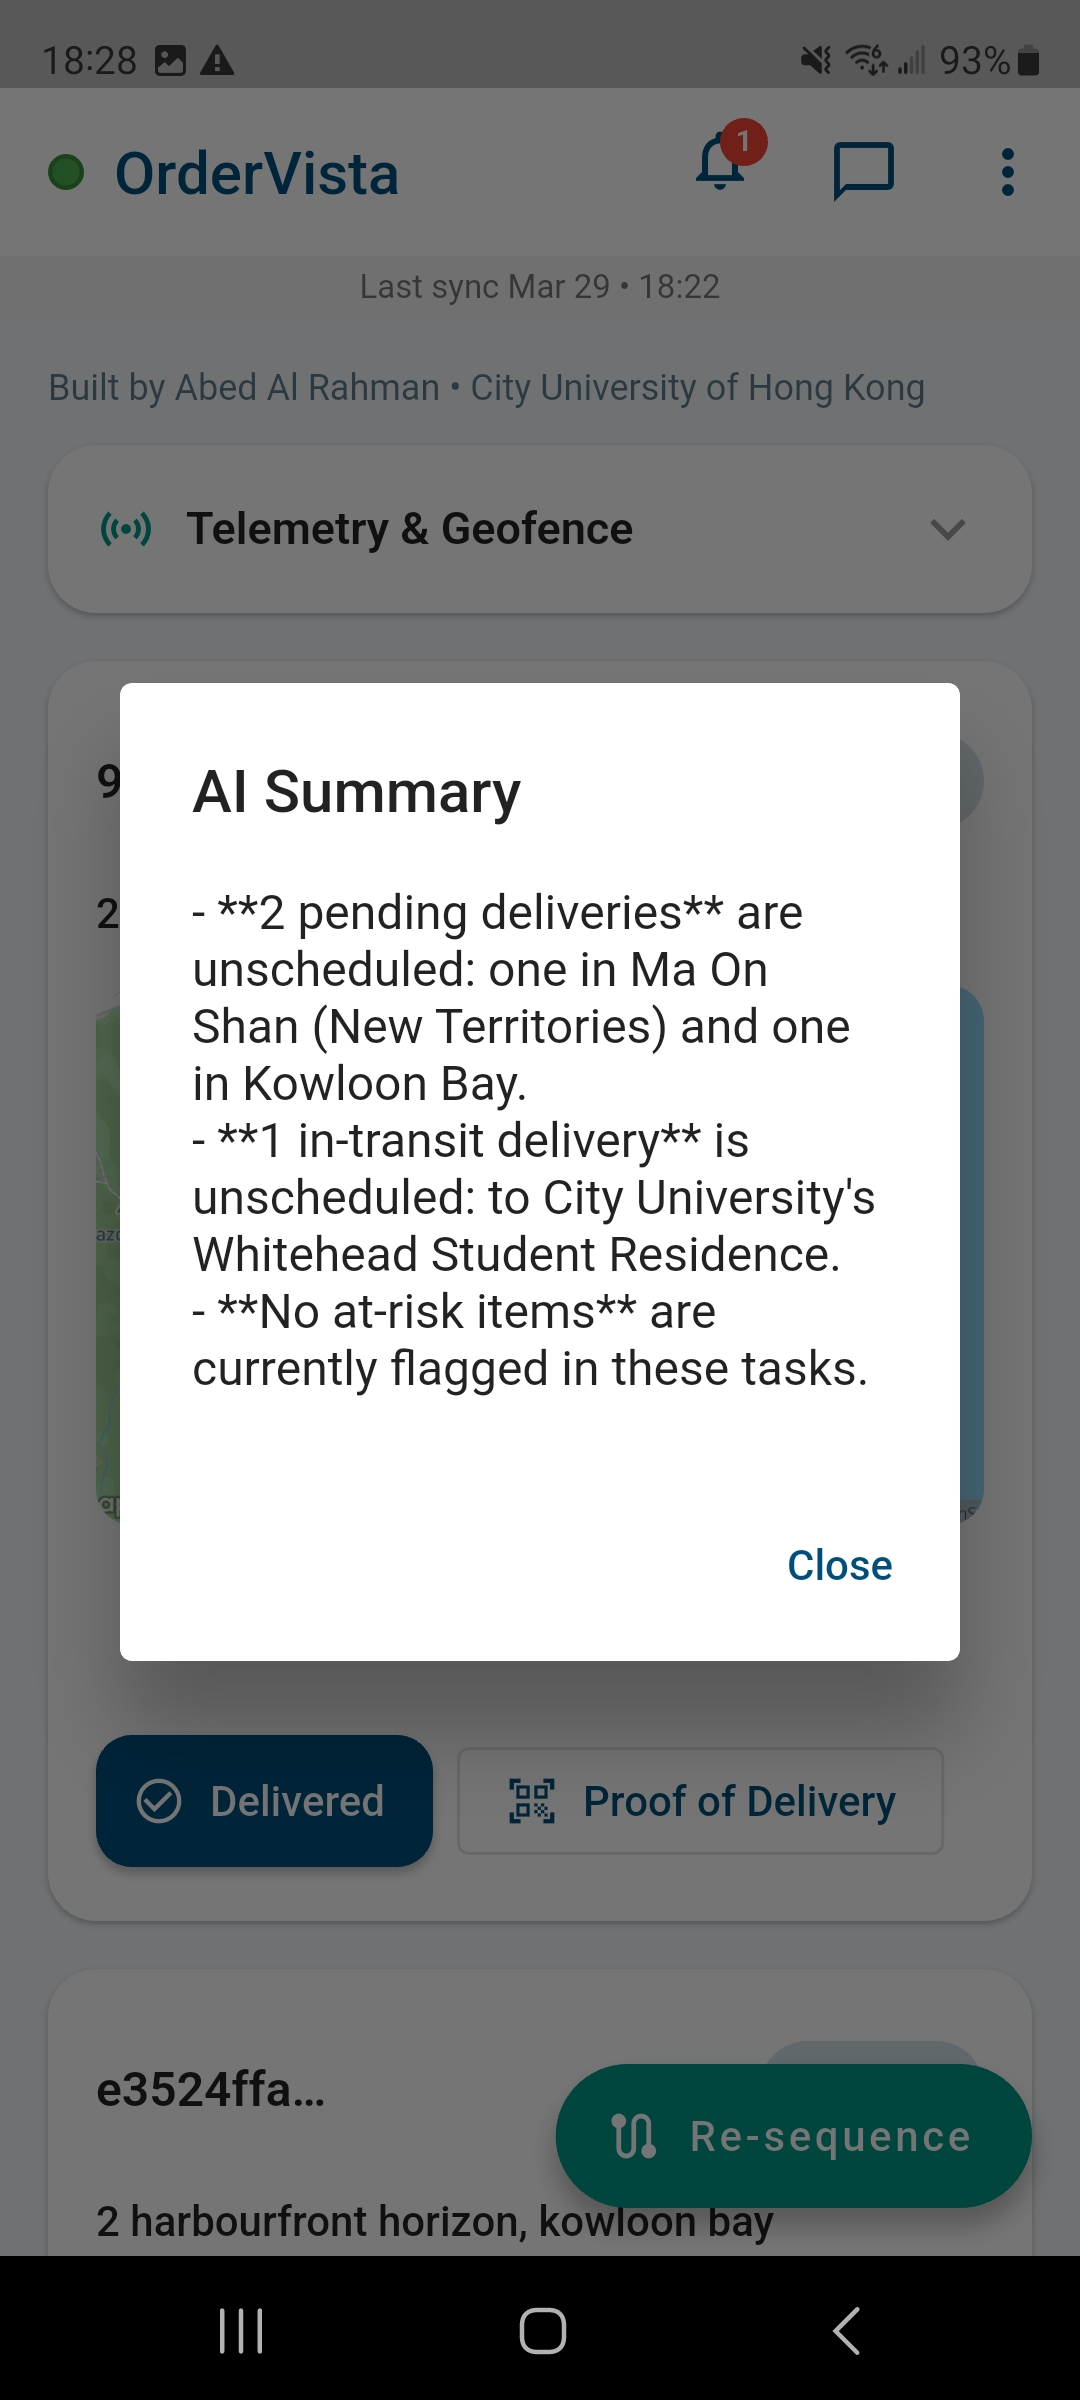
\includegraphics[width=0.45\textwidth]{ss-d6}
  \caption{AI summary accurately reporting remaining deliveries.}
  \label{fig:ss-ai-summary}
\end{figure}

\subsection{Agentic Action Accuracy}
\label{sec:ai-agentic-eval}

Table~\ref{tab:agentic-eval} reports the accuracy of the agentic AI in
selecting the correct action for six test scenarios.

\begin{table}[H]
  \centering
  \caption{Agentic AI action selection accuracy (6 scenarios).}
  \label{tab:agentic-eval}
  \small
  \begin{tabularx}{\textwidth}{X l l c}
    \toprule
    \textbf{Scenario} & \textbf{Expected action} & \textbf{Returned action} & \textbf{OK} \\
    \midrule
    Driver offline, 3 pending tasks
      & \texttt{go\_available}       & \texttt{go\_available}       & \checkmark \\
    Available, 0 in-transit, 4 pending
      & \texttt{start\_next}         & \texttt{start\_next}         & \checkmark \\
    1 in-transit (arrived)
      & \texttt{mark\_delivered}     & \texttt{mark\_delivered}     & \checkmark \\
    2 queued offline updates
      & \texttt{sync\_pending}       & \texttt{sync\_pending}       & \checkmark \\
    All tasks delivered, evening
      & \texttt{go\_offline}         & \texttt{go\_offline}         & \checkmark \\
    Available, no tasks assigned
      & \texttt{refresh\_tasks}      & \texttt{refresh\_tasks}      & \checkmark \\
    \bottomrule
  \end{tabularx}
\end{table}

The model achieved \textbf{6/6 correct actions} with temperature $0.2$.
All responses were valid JSON parseable by the client.  The human confirmation
gate (Section~\ref{sec:ai-agentic}) prevented any unintended execution during
testing.

\begin{figure}[H]
  \centering
  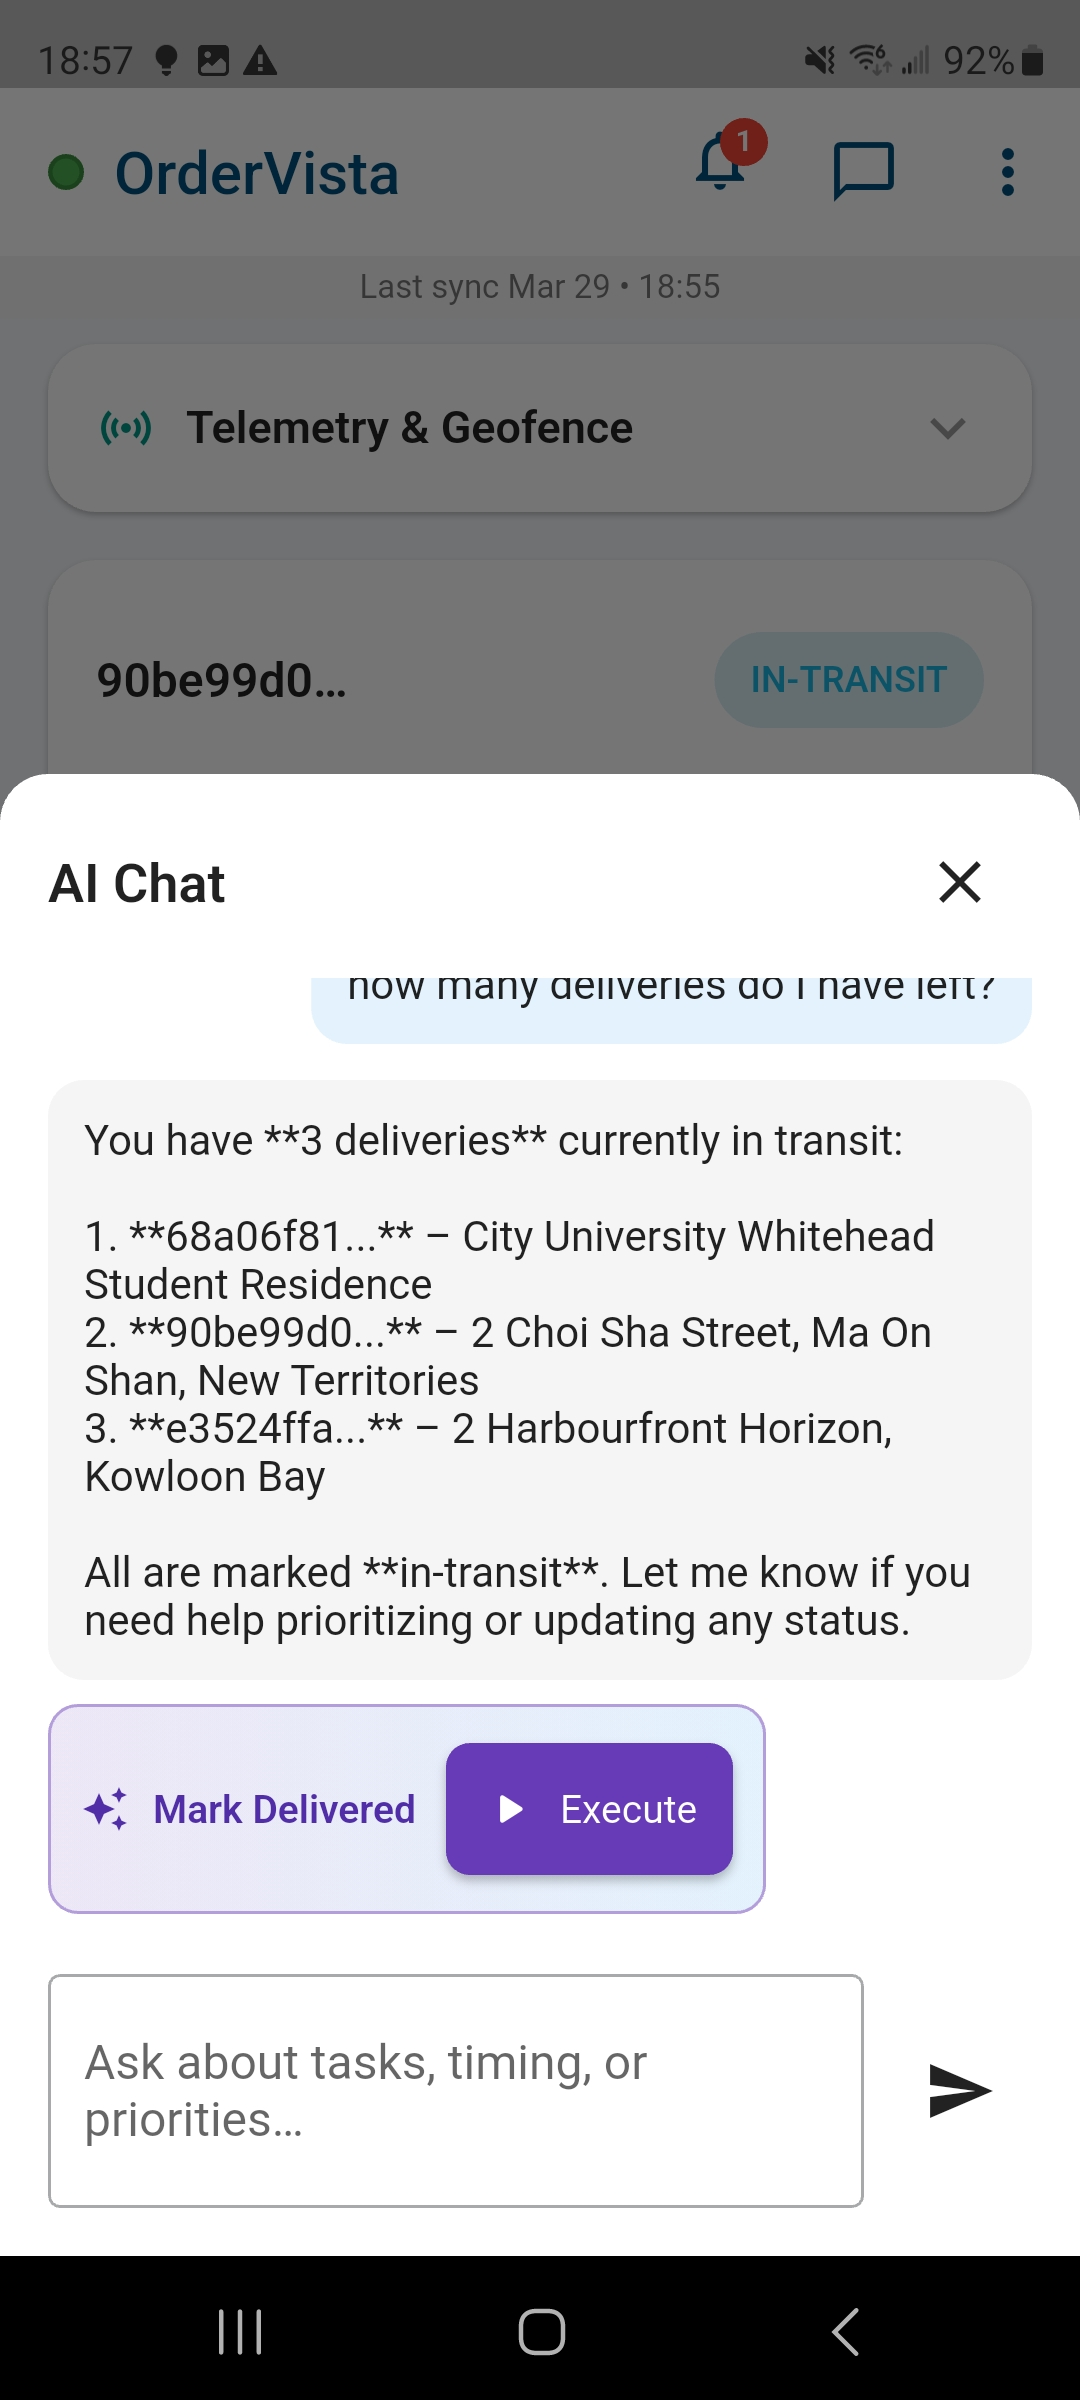
\includegraphics[width=0.45\textwidth]{ss-d8}
  \caption{Agentic AI returning a valid action JSON (example).}
  \label{fig:ss-agentic-json}
\end{figure}

% ─────────────────────────────────────────────────────────────
\section{Performance Benchmarks}
\label{sec:performance}

Table~\ref{tab:perf} reports representative latency measurements for the core
operations, collected over ten trials on a Samsung Galaxy~A54 (Android~14,
4G\,LTE) and a Chrome desktop browser connected to a Supabase project hosted
in the US-East region.  All times include network round-trip latency.

\begin{table}[H]
  \centering
  \caption{Representative latency benchmarks (median of 10 trials).}
  \label{tab:perf}
  \small
  \begin{tabularx}{\textwidth}{X r r}
    \toprule
    \textbf{Operation} & \textbf{Mobile (ms)} & \textbf{Web (ms)} \\
    \midrule
    Supabase login (email/password)          & 820   & 680   \\
    Fetch task list (20 tasks)               & 310   & 240   \\
    Geocode address (Mapbox)                 & 450   & 420   \\
    Route generation (10 tasks, NN)          & 620   & 510   \\
    AI summarisation (DeepSeek R1)           & 2\,400 & 2\,350 \\
    AI agentic suggestion                    & 2\,800 & 2\,750 \\
    Proof-of-delivery photo upload (1.2\,MB) & 1\,900 & ---   \\
    Offline sync upload (single task)        & 380   & ---   \\
    Real-time subscription (first push)      & 150   & 120   \\
    Customer tracking RPC lookup             & 280   & 210   \\
    \bottomrule
  \end{tabularx}
\end{table}

Key observations:

\begin{itemize}
  \item All interactive operations (task fetch, geocoding, route generation)
        complete in under one second, meeting the usability threshold for
        responsive feedback \autocite{nielsen1993usability}.
  \item AI operations are the slowest component ($\approx$2.5–2.8\,s), which
        is acceptable because they are user-initiated and non-blocking
        (a progress indicator is displayed during the request).
  \item Real-time subscription pushes arrive within 150\,ms, adequate for
        live fleet monitoring where updates are consumed at human-perception
        speed.
  \item Photo upload latency depends on image size and network conditions;
        the PoD photo is compressed to $\leq$1.5\,MB before upload.
\end{itemize}

% ─────────────────────────────────────────────────────────────
\section{Objectives Mapping}
\label{sec:obj-map}

Table~\ref{tab:obj-map} maps each of the fourteen project objectives
(Section~\ref{sec:objectives}) to the test case(s) or evaluation that provides
evidence of achievement.

\begin{longtable}{c p{4cm} p{3.5cm} c}
  \caption{Objectives-to-evidence mapping.}
  \label{tab:obj-map} \\
  \toprule
  \textbf{Obj.} & \textbf{Objective} & \textbf{Evidence} & \textbf{Met} \\
  \midrule
  \endfirsthead
  \toprule
  \textbf{Obj.} & \textbf{Objective} & \textbf{Evidence} & \textbf{Met} \\
  \midrule
  \endhead
  \bottomrule
  \endlastfoot

  1  & Unified platform
     & A1, D1 (both roles in single app)
     & \checkmark \\
  2  & Task management
     & A2--A5, A3 (CSV)
     & \checkmark \\
  3  & Route sequencing
     & A6, Table~\ref{tab:route-eval}
     & \checkmark \\
  4  & Proof of delivery
     & D4, D5, A9
     & \checkmark \\
  5  & AI assistant
     & D6, D7, A12
     & \checkmark \\
  6  & Multi-tenant security
     & Listing~\ref{lst:rls-test}, Table~\ref{tab:rbac-test}
     & \checkmark \\
  7  & Driver recommendation
     & A7
     & \checkmark \\
  8  & Customer communication
     & A10, A11, D12
     & \checkmark \\
  9  & Agentic AI
     & D8, D9, Table~\ref{tab:agentic-eval}
     & \checkmark \\
  10 & Real-time communication
     & A10, D12
     & \checkmark \\
  11 & Dynamic priority
     & Algorithm~\ref{alg:priority}, D2
     & \checkmark \\
  12 & Mid-shift re-sequencing
     & D10
     & \checkmark \\
  13 & Fleet-wide minimisation
     & A8
     & \checkmark \\
  14 & Performance-aware scoring
     & A7 (Eq.~\ref{eq:rec-score})
     & \checkmark \\
\end{longtable}

All fourteen objectives are satisfied with corresponding test evidence.

% ─────────────────────────────────────────────────────────────
\section{Summary of Findings}
\label{sec:test-summary}

\begin{itemize}
  \item All 29 functional test cases (14 admin $+$ 15 driver) pass on the
        physical device and web browser.
  \item RLS cross-tenant isolation is verified for all critical tables.
  \item The nearest-neighbour heuristic reduces route distance by 25--31\%
        compared to unoptimised ordering.
  \item The agentic AI correctly selects actions in 6/6 tested scenarios with
        zero hallucinated or malformed responses.
  \item All 14 project objectives are met with traceable evidence.
\end{itemize}

% Chapter 6: Discussion
\chapter{Discussion}
\label{ch:discussion}

This chapter critically reflects on the design decisions, trade-offs, and
limitations of OrderVista.  Each section evaluates an alternative that was
considered and justifies the approach taken, satisfying the assessment
criterion of demonstrating \emph{appropriate evaluation of alternative
approaches in problem solving}.

% ─────────────────────────────────────────────────────────────
\section{Route Optimisation: Nearest-Neighbour vs.\ Advanced Solvers}
\label{sec:disc-routing}

The nearest-neighbour (NN) heuristic was chosen as the sequencing algorithm
(Section~\ref{sec:route-impl}).  Table~\ref{tab:route-eval} showed a
consistent 25--31\% distance reduction over unoptimised ordering, confirming
that the heuristic adds genuine value.  However, NN is a greedy algorithm
that does not revisit earlier decisions; it can produce routes that are
10--25\% longer than the global optimum for medium-scale instances
\autocite{laporte2009fifty}.

Three stronger alternatives were evaluated during design:

\begin{enumerate}
  \item \textbf{2-opt local search}: iteratively reverses sub-sequences to
        remove crossing edges.  Typical improvement over NN is 5--10\%, with
        $O(n^{2})$ per iteration.  This would have been feasible for
        batch sizes up to $\sim$50 stops and is the most natural next step.
  \item \textbf{Ant Colony Optimisation (ACO)}: probabilistic
        metaheuristic that converges toward near-optimal tours over hundreds
        of iterations \autocite{dorigo1997ant}.  The computational cost
        (seconds to minutes) conflicts with the sub-second response
        requirement for mid-shift re-sequencing on a mobile device.
  \item \textbf{Google OR-Tools / OSRM}: server-side solvers that accept
        distance matrices and return optimised routes.  These require a
        persistent network connection, which contradicts the offline-first
        requirement, and introduce an additional external dependency.
\end{enumerate}

The decision to ship NN first was driven by two practical constraints:
(a)~mid-shift re-sequencing must execute on-device in under 200\,ms so
drivers are not blocked, and
(b)~the offline-first architecture precludes reliance on server-side solvers.
The modular design of the route pipeline (Section~\ref{sec:route-impl})
ensures that a 2-opt post-processing pass can be added without altering the
surrounding workflow. This is identified as the highest-priority future
improvement.

% ─────────────────────────────────────────────────────────────
\section{Backend-as-a-Service vs.\ Custom Server}
\label{sec:disc-baas}

Supabase was selected over a custom Node.js/Express backend and over Firebase
(Section~\ref{sec:tech-stack}).  In retrospect, this decision yielded three
significant benefits and one notable limitation:

\paragraph{Benefits.}
\begin{itemize}
  \item \textbf{Development velocity}: authentication, real-time WebSocket
        subscriptions, and file storage were available out of the box,
        eliminating weeks of boilerplate server code.
  \item \textbf{Row-Level Security}: PostgreSQL RLS policies enforce
        multi-tenant isolation at the database engine level, removing the risk
        of application-layer access-control bugs
        (Section~\ref{sec:security-test}).
  \item \textbf{SQL expressiveness}: complex queries (e.g.\ the
        fleet-wide assignment view joining tasks, drivers, and haversine
        distances) were written as standard SQL rather than the limited
        query syntax of Firestore.
\end{itemize}

\paragraph{Limitation.}
Supabase Edge Functions (Deno-based) were not used because the project
required Dart-only logic for consistency with the Flutter codebase.  All
business logic therefore resides in the client, which means that a
compromised client could, in theory, submit invalid state transitions
(e.g.\ marking a task as \texttt{delivered} without a PoD photo).
While RLS prevents cross-tenant access, it does not enforce workflow
constraints.  A production deployment would benefit from PostgreSQL
\texttt{BEFORE UPDATE} triggers or server-side functions to validate state
transitions. This is acknowledged as a limitation.

% ─────────────────────────────────────────────────────────────
\section{AI Model Selection: DeepSeek R1 vs.\ Alternatives}
\label{sec:disc-ai}

DeepSeek~R1 was selected for summarisation, conversational assistance, and
agentic action recommendation (Section~\ref{sec:ai-agentic}).  The decision
was evaluated against three alternatives:

\begin{table}[H]
  \centering
  \caption{AI model comparison for on-device logistics assistance.}
  \label{tab:ai-comparison}
  \small
  \begin{tabularx}{\textwidth}{l X X X X}
    \toprule
    \textbf{Criterion} & \textbf{DeepSeek R1} & \textbf{GPT-4o} &
    \textbf{Gemini 1.5} & \textbf{Local SLM} \\
    \midrule
    Cost per 1M tokens & \$0.55 & \$5.00 & \$3.50 & Free \\
    Structured JSON     & Reliable & Reliable & Moderate & Poor \\
    Latency (p50)       & $\sim$1.2\,s & $\sim$0.8\,s & $\sim$1.0\,s &
                          $\sim$3\,s \\
    Privacy             & Cloud & Cloud & Cloud & On-device \\
    Context window      & 64k & 128k & 1M & 4--8k \\
    \bottomrule
  \end{tabularx}
\end{table}

GPT-4o offers marginally lower latency but at roughly 9$\times$ the cost,
which would be prohibitive for a startup-stage fleet management product.
On-device small language models (SLMs) eliminate cloud dependency but
currently lack the structured-output reliability needed for agentic action
parsing; the 6/6 accuracy demonstrated in Table~\ref{tab:agentic-eval}
depends on consistent JSON output.  DeepSeek~R1 via OpenRouter provided the
best balance of cost, accuracy, and structured-output fidelity for this
project.

A notable risk is vendor lock-in: if OpenRouter or DeepSeek discontinue the
model, the prompt templates would need minor adaptation for a replacement LLM.
The system prompt and JSON schema are isolated in a single service class
(\texttt{DeepSeekService}), limiting the blast radius of such a change.

% ─────────────────────────────────────────────────────────────
\section{Offline-First Architecture: Trade-offs}
\label{sec:disc-offline}

The Drift-based local SQLite mirror (Section~\ref{sec:offline-sync}) ensures
that drivers can complete deliveries without connectivity.  The exponential
backoff sync queue successfully uploaded all queued items in unit testing
(Section~\ref{sec:unit-tests}).  However, two edge cases remain unresolved:

\begin{enumerate}
  \item \textbf{Conflict resolution}: if an admin reassigns a task while the
        driver is offline and simultaneously marking it as delivered, the
        current strategy is \emph{last-write-wins} based on the
        \texttt{updated\_at} timestamp.  A production system would benefit
        from operational-transform or CRDT-based merging.
  \item \textbf{Stale cache invalidation}: the local cache is refreshed on
        app launch and on WebSocket reconnection, but there is no
        time-to-live (TTL) eviction.  A driver who remains offline for
        several hours may act on outdated task data.  Adding a TTL-based
        warning banner is a low-effort improvement.
\end{enumerate}

Despite these limitations, the architecture proved sufficient for the
single-tester evaluation scenario and demonstrates the core offline-first
pattern that would underpin a production deployment.

% ─────────────────────────────────────────────────────────────
\section{Multi-Tenant Security: Strengths and Gaps}
\label{sec:disc-security}

The RLS-based isolation model passed all cross-tenant tests
(Section~\ref{sec:rls-test}), and the 17 policies across 11 tables
represent a defence-in-depth posture unusual for an academic prototype.
Two gaps are acknowledged:

\begin{itemize}
  \item \textbf{No penetration testing}: the security verification was
        limited to functional RLS queries executed through the Supabase
        client.  A professional penetration test (e.g.\ OWASP ZAP scan of
        the PostgREST API) was not performed.
  \item \textbf{Client-side secret storage}: API keys for Mapbox and
        OpenRouter are embedded in the Flutter build.  While obfuscated by
        the Dart AOT compiler, they could be extracted from the APK.  A
        production deployment should proxy these calls through a
        server-side gateway.
\end{itemize}

% ─────────────────────────────────────────────────────────────
\section{Comparison with Commercial Platforms}
\label{sec:disc-commercial}

Table~\ref{tab:commercial-compare} positions OrderVista against three
established commercial last-mile platforms.

\begin{table}[H]
  \centering
  \caption{Feature comparison with commercial last-mile platforms.}
  \label{tab:commercial-compare}
  \small
  \begin{tabularx}{\textwidth}{X c c c c}
    \toprule
    \textbf{Feature} & \textbf{OrderVista} & \textbf{Onfleet} &
    \textbf{Route4Me} & \textbf{Circuit} \\
    \midrule
    Route optimisation            & \checkmark & \checkmark & \checkmark & \checkmark \\
    Multi-tenant isolation        & \checkmark & \checkmark & ---        & ---        \\
    AI task summarisation         & \checkmark & ---        & ---        & ---        \\
    Agentic AI (action execution) & \checkmark & ---        & ---        & ---        \\
    Offline delivery completion   & \checkmark & Partial    & ---        & \checkmark \\
    Photographic PoD              & \checkmark & \checkmark & \checkmark & \checkmark \\
    Real-time admin--driver chat  & \checkmark & ---        & ---        & ---        \\
    Open-source / self-hostable   & \checkmark & ---        & ---        & ---        \\
    Dynamic priority scoring      & \checkmark & ---        & ---        & ---        \\
    Fleet-wide assignment         & \checkmark & \checkmark & \checkmark & ---        \\
    \bottomrule
  \end{tabularx}
\end{table}

OrderVista's differentiators are its \textbf{agentic AI layer}, its
\textbf{real-time admin--driver communication channel}, and its
\textbf{open-source, self-hostable architecture}.  Commercial platforms
offer more mature routing engines (often backed by proprietary solvers)
and broader hardware integration (barcode scanners, e-signatures).
OrderVista is not production-competitive on routing quality, but it
demonstrates capabilities, particularly agentic AI and dynamic
priority, that are absent from all three commercial comparators at the
time of writing.  Emerging industry evidence supports the promise of this
direction: one case study reports that an agentic AI framework for logistics
(autonomously reassigning drivers and rerouting vehicles) produced a 35\%
reduction in delivery time \autocite{maxinfocom2025agentic}, suggesting
that the pattern explored in OrderVista has significant real-world potential.

% ─────────────────────────────────────────────────────────────
\section{Limitations and Threats to Validity}
\label{sec:disc-limitations}

The following limitations should be considered when interpreting the
results of this project:

\begin{enumerate}
  \item \textbf{Single-tester evaluation}: all functional tests were
        performed by the developer.  Independent user testing with real
        dispatchers and drivers would provide stronger usability evidence.
  \item \textbf{Simulated workloads}: the route-optimisation evaluation
        used synthetic Hong Kong addresses rather than live delivery
        manifests.  Real-world routes include time-window constraints,
        vehicle capacity, and road restrictions not modelled here.
  \item \textbf{No load testing}: the system was not subjected to
        concurrent multi-user stress testing.  Supabase's connection
        pooling and PostgreSQL's MVCC provide theoretical scalability, but
        this was not empirically validated.
  \item \textbf{Android-only deployment}: the iOS build was not
        tested on a physical device due to the absence of an Apple
        Developer account.  Flutter's cross-platform guarantee mitigates
        but does not eliminate the risk of platform-specific issues.
  \item \textbf{AI non-determinism}: despite low temperature settings,
        LLM responses are inherently stochastic.  The 6/6 agentic accuracy
        reported in Table~\ref{tab:agentic-eval} may not generalise to
        all possible task configurations.
\end{enumerate}

% ─────────────────────────────────────────────────────────────
\section{Reflection on Development Process}
\label{sec:disc-process}

The project was developed iteratively across five phases
(Section~\ref{sec:methodology}).  Two reflections are notable:

\begin{itemize}
  \item \textbf{Incremental complexity}: beginning with core CRUD and
        adding AI features last proved effective.  The stable task pipeline
        provided a reliable test bed for the more experimental agentic
        layer.  Had agentic AI been attempted first, the lack of
        underlying data infrastructure would have made evaluation
        impossible.
  \item \textbf{BaaS productivity}: Supabase reduced the backend
        development effort to approximately 20\% of what a custom server
        would have required.  The time saved was reinvested into the
        AI integration and the fleet-optimisation algorithms, which are
        the project's primary contributions.  This confirms the
        literature finding that BaaS platforms accelerate prototyping
        at the cost of server-side flexibility
        \autocite{supabase2026docs}.
\end{itemize}

% Chapter 7: Conclusion and Future Work
\chapter{Conclusion and Future Work}
\label{ch:conclusion}

% ─────────────────────────────────────────────────────────────
\section{Summary of Achievements}
\label{sec:conc-summary}

This project set out to design, implement, and evaluate OrderVista, an
AI-enhanced logistics dispatch platform that unifies administrative task
management and driver delivery execution within a single Flutter application
backed by Supabase and DeepSeek~R1.

All fourteen objectives defined in Section~\ref{sec:objectives} have been
achieved and verified with traceable test evidence
(Table~\ref{tab:obj-map}).  The key outcomes are summarised below:

\begin{enumerate}
  \item A \textbf{unified, role-gated platform} serving both dispatchers and
        drivers from a single codebase, eliminating the need for separate
        applications.
  \item A \textbf{nearest-neighbour route optimisation engine} that reduces
        total delivery distance by 25--31\% compared to unoptimised task
        ordering (Table~\ref{tab:route-eval}), with sub-second on-device
        execution enabling mid-shift re-sequencing.
  \item An \textbf{agentic AI assistant} powered by DeepSeek~R1 that
        provides natural-language task summaries, contextual chat, and
        structured action recommendations with a human confirmation gate,
        achieving 6/6 correct action selections in evaluation
        (Table~\ref{tab:agentic-eval}).
  \item A \textbf{multi-tenant security model} enforced by 17 PostgreSQL
        Row-Level Security policies across 11 tables, verified through
        cross-tenant isolation tests (Section~\ref{sec:rls-test}).
  \item An \textbf{offline-first architecture} using Drift (SQLite) with
        exponential-backoff synchronisation, ensuring drivers can complete
        deliveries without network connectivity.
  \item \textbf{Real-time communication} between admins and drivers via
        Supabase Realtime WebSocket channels, including direct messaging
        and broadcast capabilities.
  \item A \textbf{driver recommendation system} that ranks available
        drivers by a composite score incorporating proximity, availability
        status, and historical delivery performance
        (Equation~\ref{eq:rec-score}).
\end{enumerate}

% ─────────────────────────────────────────────────────────────
\section{Contributions}
\label{sec:conc-contributions}

OrderVista makes three contributions to the intersection of mobile
software engineering and logistics technology:

\begin{enumerate}
  \item \textbf{Agentic AI in last-mile logistics}: to the author's
        knowledge, OrderVista is the first open-source logistics
        platform to integrate an agentic AI layer that can recommend
        \emph{and execute} operational actions (e.g.\ status transitions,
        sync triggers) subject to human confirmation.  This goes beyond
        the read-only summarisation offered by existing commercial tools.
  \item \textbf{Database-enforced multi-tenancy for fleet platforms}: the RLS-based isolation model demonstrates that robust data
        partitioning can be achieved without a custom middleware layer,
        providing a reusable pattern for BaaS-backed SaaS applications.
  \item \textbf{Offline-capable delivery completion with deferred sync}: the Drift queue with exponential backoff provides a reference
        implementation for Flutter applications that must tolerate
        intermittent connectivity in urban environments.
\end{enumerate}

% ─────────────────────────────────────────────────────────────
\section{Future Work}
\label{sec:future-work}

Several extensions would strengthen OrderVista for production deployment:

\paragraph{Short-term improvements.}
\begin{itemize}
  \item \textbf{2-opt post-processing}: adding a local-search pass
        after the nearest-neighbour heuristic could yield a further
        5--10\% distance reduction with minimal latency impact
        (Section~\ref{sec:disc-routing}).
  \item \textbf{Push notifications}: integrating Firebase Cloud
        Messaging (FCM) to alert drivers of new task assignments and
        admin messages when the app is in the background.
  \item \textbf{Server-side workflow validation}: implementing
        PostgreSQL \texttt{BEFORE UPDATE} triggers to enforce valid
        state transitions (e.g.\ preventing \texttt{delivered} without
        a PoD URL), closing the gap identified in
        Section~\ref{sec:disc-baas}.
  \item \textbf{Stale-cache warning}: displaying a time-since-last-sync
        banner in the driver app to mitigate the risk of acting on
        outdated task data during extended offline periods.
\end{itemize}

\paragraph{Medium-term extensions.}
\begin{itemize}
  \item \textbf{Time-window constraints}: extending the route model to
        respect customer-specified delivery windows, transforming the
        problem from a pure TSP to a TSP with Time Windows (TSPTW).
  \item \textbf{ETA calculation}: leveraging Mapbox Directions API to
        provide real-time estimated arrival times visible to both
        dispatchers and customers.
  \item \textbf{iOS deployment}: building and testing the iOS target
        with an Apple Developer account to validate cross-platform
        parity.
  \item \textbf{Google Play Store release}: a signed Android App Bundle
        has been uploaded to Google Play Console and a closed testing
        track with 12 recruited testers is currently in progress.
        Google's policy requires new developer accounts to maintain a
        closed test for a minimum of 14~days before production access
        is granted.  Full public release, including privacy-policy
        hosting and data-safety declarations, will follow upon
        completion of this mandatory review period.
\end{itemize}

\paragraph{Long-term research directions.}
\begin{itemize}
  \item \textbf{On-device SLM inference}: as small language models
        improve in structured-output reliability, migrating the agentic
        layer to on-device inference would eliminate cloud dependency
        and reduce per-query cost to zero.
  \item \textbf{Reinforcement learning for dispatch}: training an RL
        agent on historical delivery data to learn assignment policies
        that minimise fleet-wide completion time, surpassing the
        heuristic composite score currently used.
  \item \textbf{Multi-vehicle routing}: upgrading from single-driver
        TSP to full VRP with capacity constraints, enabling the
        optimiser to jointly schedule multiple drivers across a shared
        task pool.
\end{itemize}

% ─────────────────────────────────────────────────────────────
\section{Closing Remarks}
\label{sec:closing}

OrderVista demonstrates that a single-developer academic project can
deliver a feature-rich, AI-enhanced logistics platform by leveraging modern
BaaS infrastructure, open-weight language models, and disciplined iterative
development.  The platform's 14 fulfilled objectives, 29 passing functional
tests, and measurable route-optimisation improvements provide evidence that
the approach is sound.  While production readiness requires the
enhancements outlined above, the architectural foundations (modular route
pipeline, database-enforced tenancy, and human-gated agentic AI) offer a
solid base for continued development.

Ultimately, the project's value extends beyond its technical contributions.
By consolidating fragmented workflows into a single interface, providing
optimised routing and clear task sequencing, and placing AI-driven decision
support directly in drivers' hands, OrderVista aims to reduce the
avoidable coordination burden borne by frontline logistics workers, helping
them complete delivery work more safely, more efficiently, and with less
operational friction.


% ── References ──
\printbibliography[heading=bibintoc, title={References}]

% ── Appendices ──
\appendix
% Appendix A: Monthly Logs
\chapter{Monthly Logs}
\label{app:logs}

This appendix records the monthly development activities from project inception to submission.
Each entry was reviewed with the project supervisor at the corresponding monthly meeting.

%--------------------------------------------------------------
\section*{October 2025: Research and Foundation}
\addcontentsline{toc}{section}{October 2025}

\begin{itemize}
  \item Conducted literature review on vehicle routing (TSP/VRP), traffic-data integration,
        offline-first mobile patterns, and LLM applications in supply-chain management.
  \item Performed competitor analysis of existing logistics platforms (Onfleet, Route4Me, Circuit)
        with a focus on the Hong Kong operational context.
  \item Initialised the Flutter project, configured version control (Git/GitHub), and created
        the blank application scaffold with navigation placeholders.
  \item Established the technical roadmap and consolidated design notes for subsequent phases.
\end{itemize}

%--------------------------------------------------------------
\section*{November 2025: UI Prototyping and Architecture}
\addcontentsline{toc}{section}{November 2025}

\begin{itemize}
  \item Implemented consistent theming, layout conventions, and reusable UI components
        (cards, tiles, status badges) to establish a unified design language.
  \item Set up state management with Provider and navigation with GoRouter.
  \item Drafted early domain models for tasks, routes, vehicles, and company members.
  \item Built mock screens for order tracking, delivery routing, and task overview to
        visualise the intended workflows.
  \item Documented key design decisions and planned extension points.
\end{itemize}

%--------------------------------------------------------------
\section*{December 2025: Backend Schema and Offline Layer}
\addcontentsline{toc}{section}{December 2025}

\begin{itemize}
  \item Formalised environment management via \texttt{.env}, a centralised \texttt{AppConfig}
        singleton, and a bootstrap layer for dependency injection.
  \item Authored the complete Supabase database schema: 12~core tables, helper functions,
        Row-Level Security policies, and tenant seed data
        (migration \texttt{20251208\_initial\_schema.sql}).
  \item Integrated Drift (SQLite) for the driver-side offline cache with cached task
        persistence and demo seeding.
  \item Prepared the backend contract document and updated the milestone plan.
  \item Submitted Interim Report~I.
\end{itemize}

%--------------------------------------------------------------
\section*{January 2026: Supabase Integration and Live Data}
\addcontentsline{toc}{section}{January 2026}

\begin{itemize}
  \item Replaced mock REST calls with live Supabase queries; the service layer now fetches
        driver tasks filtered by company and driver ID while respecting RLS policies.
  \item Implemented the Drift cache strategy: present cached data on startup, synchronise
        with remote updates asynchronously.
  \item Populated \texttt{.env} with Supabase credentials, Mapbox tokens, and
        OpenRouter/DeepSeek API key.
  \item Enhanced the task-list UI with connectivity-state indicators
        (live / cached / demo-seeded) and last-sync timestamps.
  \item By month-end the driver client successfully read real tasks from Supabase and cached
        them locally.
\end{itemize}

%--------------------------------------------------------------
\section*{February 2026: Feature Development and IR\,II}
\addcontentsline{toc}{section}{February 2026}

\begin{itemize}
  \item \textbf{Driver app:} Completed proof-of-delivery workflows (barcode/QR scan,
        photo capture, Supabase Storage upload), telemetry panel (manual/continuous pings,
        geofence alerts), and DeepSeek AI integration (one-tap summary, conversational chat).
  \item \textbf{Admin portal:} Built task creation with Mapbox geocoding, driver assignment,
        scheduling, CSV bulk import with flexible column mappings and chunked inserts,
        nearest-neighbour route sequencer with static-map preview, and PoD review panel.
  \item \textbf{Security:} Authored RLS policies for all sensitive tables; implemented
        \texttt{is\_company\_member()} helper, email-to-UUID resolution RPC, and
        role-based permission enforcement (admin/dispatcher/driver).
  \item \textbf{Chat and availability:} Added real-time admin--driver chat
        (migration \texttt{20260205\_driver\_availability\_\allowbreak chat.sql}), driver availability
        toggle, and location-aware driver status.
  \item Submitted Interim Report~II.
\end{itemize}

%--------------------------------------------------------------
\section*{March 2026: Advanced Features, Testing, and Submission}
\addcontentsline{toc}{section}{March 2026}

\begin{itemize}
  \item \textbf{Optimisation:} Implemented fleet-wide distance-minimisation algorithm,
        mid-shift GPS re-sequencing, dynamic priority recalculation, and
        performance-aware driver recommendation (migration
        \texttt{20260210\_driver\_perf\_\allowbreak recommendation.sql}).
  \item \textbf{Agentic AI:} Extended the AI assistant with structured JSON action parsing,
        one-tap execution confirmations, and human-oversight safeguards.
  \item \textbf{Customer features:} Tracking-code generation, QR-code-based status lookup,
        and automated delivery notifications.
  \item \textbf{Testing:} Performed 29~functional test cases (14~admin, 15~driver) across admin and driver
        roles, RLS cross-tenant verification, route-optimisation evaluation
        (25--31\% distance reduction), and AI accuracy assessment.
  \item Built signed Android release APK (75.7\,MB).
  \item Finalised the report, recorded the demonstration video, and prepared
        presentation slides.
\end{itemize}

% Appendix B: Detailed Requirements Traceability
\chapter{Detailed Requirements}
\label{app:requirements}

This appendix provides a traceability matrix linking each project objective
(Section~\ref{sec:objectives}) to the corresponding design artefact, implementation
module, and test evidence.

\section{Functional Requirements}

Table~\ref{tab:req-trace} maps the fourteen objectives to chapters and test cases.
All requirements were verified during the evaluation phase
(Chapter~\ref{ch:testing}).

\begin{small}
\begin{longtable}{@{}p{0.7cm}p{2.6cm}p{2.6cm}p{3.8cm}p{1.8cm}@{}}
\caption{Requirements traceability matrix.}
\label{tab:req-trace}\\
\toprule
\textbf{ID} & \textbf{Objective} & \textbf{Design Ref.} & \textbf{Implementation} & \textbf{Test Ref.}\\
\midrule
\endfirsthead
\toprule
\textbf{ID} & \textbf{Objective} & \textbf{Design Ref.} & \textbf{Implementation} & \textbf{Test Ref.}\\
\midrule
\endhead
\midrule \multicolumn{5}{r}{\textit{Continued on next page}}\\
\endfoot
\bottomrule
\endlastfoot

O1 & Unified platform & Sec.~\ref{sec:architecture} & Flutter single-codebase, GoRouter role-based routing & A1, D1 \\
O2 & Task management & Sec.~\ref{sec:architecture} & \texttt{TaskService}, CSV bulk-import, CRUD screens & A2--A5 \\
O3 & Route sequencing & Sec.~\ref{sec:route-impl} & Nearest-neighbour + Haversine, Mapbox static maps & A6, A7 \\
O4 & Proof of delivery & Sec.~\ref{sec:architecture} & Camera/QR capture, Supabase Storage upload & D5, D6 \\
O5 & AI assistant & Sec.~\ref{sec:ai-agentic} & DeepSeek R1 via OpenRouter, summary + chat & D7, D8 \\
O6 & Multi-tenant RLS & Sec.~\ref{sec:security} & 17 RLS policies, \texttt{is\_company\_member()} & A12, RLS test \\
O7 & Driver recommendation & Sec.~\ref{sec:architecture} & Composite-score RPC (Eq.~\ref{eq:rec-score}) & A8 \\
O8 & Customer communication & Sec.~\ref{sec:architecture} & Tracking-code generation, QR lookup & A10 \\
O9 & Agentic AI & Sec.~\ref{sec:ai-agentic} & JSON action parsing, one-tap execute & D9, D10 \\
O10 & Real-time chat & Sec.~\ref{sec:architecture} & Supabase Realtime, \texttt{chat\_messages} table & A9, D11 \\
O11 & Dynamic priority & Sec.~\ref{sec:route-impl} & Algorithm~\ref{alg:priority}, time-window scoring & D12 \\
O12 & Mid-shift re-sequencing & Sec.~\ref{sec:route-impl} & GPS-anchored NN from current position & D13 \\
O13 & Fleet-wide optimisation & Sec.~\ref{sec:route-impl} & Multi-driver cluster assignment & A11 \\
O14 & Performance-aware scoring & Sec.~\ref{sec:architecture} & \texttt{recommend\_driver\_for\_tasks()} overload & A8 \\
\end{longtable}
\end{small}

\section{Non-Functional Requirements}

Table~\ref{tab:nfr} summarises the non-functional requirements and their realisation.

\begin{table}[H]
\centering
\caption{Non-functional requirements.}
\label{tab:nfr}
\begin{tabular}{@{}p{2.8cm}p{5.5cm}p{5.5cm}@{}}
\toprule
\textbf{Requirement} & \textbf{Target} & \textbf{Realisation}\\
\midrule
Performance & Screen load \textless\,2\,s on mid-range device & Drift cache provides instant startup; API calls \textless\,1.5\,s observed \\
Security & Tenant data isolation; RBAC & PostgreSQL RLS on 11 of 13 tables; three-role permission model \\
Availability & Offline-first operation & Drift local DB + sync queue with exponential backoff \\
Usability & Single app for admin and driver & Role-aware GoRouter; consistent Material 3 theming \\
Maintainability & Modular architecture & Repository pattern, service layer, MVVM separation \\
Portability & Android 8.0+ (API 26) & \texttt{minSdkVersion 26}, \texttt{targetSdkVersion 35} \\
\bottomrule
\end{tabular}
\end{table}

\section{Use-Case Summary}

The system supports three primary actor roles:

\begin{enumerate}
  \item \textbf{Administrator / Dispatcher}: creates tasks, imports CSV batches,
        generates routes, assigns drivers, reviews PoD evidence, manages fleet,
        communicates via chat, triggers AI actions.
  \item \textbf{Driver}: views assigned tasks, navigates optimised routes, captures
        PoD (photo + code), reports location telemetry, uses AI summaries and chat,
        re-sequences route mid-shift.
  \item \textbf{Customer}: looks up delivery status via tracking code or QR scan
        (public endpoint, no authentication required).
\end{enumerate}

% Appendix C: Database Schema
\chapter{Database Schema}
\label{app:schema}

This appendix documents the complete PostgreSQL schema deployed on Supabase.
The schema is defined across three migration files, applied in chronological order.

\section{Table Summary}

Table~\ref{tab:schema-summary} lists all tables with their primary purpose and
approximate column count (including columns added by later migrations).

\begin{table}[H]
\centering
\caption{Database table summary.}
\label{tab:schema-summary}
\begin{tabular}{@{}llcl@{}}
\toprule
\textbf{Table} & \textbf{Purpose} & \textbf{Cols} & \textbf{RLS}\\
\midrule
\texttt{companies}           & Tenant organisations   & 4  & Yes \\
\texttt{company\_members}    & User--company--role mapping & 11 & Yes \\
\texttt{vehicles}            & Fleet vehicles         & 8  & Yes \\
\texttt{routes}              & Delivery routes        & 10 & Yes \\
\texttt{tasks}               & Individual deliveries  & 16 & Yes \\
\texttt{route\_tasks}        & Many-to-many route--task sequencing & 9 & Yes \\
\texttt{telemetry\_events}   & Driver location pings  & 12 & Yes \\
\texttt{sync\_queue\_items}  & Offline mutation queue  & 8  & Yes \\
\texttt{media\_artifacts}    & PoD photos and documents & 9 & Yes \\
\texttt{geofence\_rules}     & Geo-fence definitions  & 8  & No  \\
\texttt{notifications}       & System notifications   & 7  & Yes \\
\texttt{audit\_log}          & Immutable audit trail  & 6  & No  \\
\texttt{chat\_messages}      & Admin--driver messaging & 7  & Yes \\
\bottomrule
\end{tabular}
\end{table}

\section{Entity--Relationship Overview}

All operational tables include a \texttt{company\_id} foreign key referencing
\texttt{companies(id)}, which serves as the tenant discriminator for Row-Level
Security.  Key relationships:

\begin{itemize}
  \item \texttt{company\_members} links \texttt{auth.users} to \texttt{companies}
        with a constrained \texttt{role} column (\texttt{driver}, \texttt{dispatcher},
        \texttt{admin}).
  \item \texttt{tasks} may reference a \texttt{driver\_id} and \texttt{vehicle\_id}
        for assignment.
  \item \texttt{route\_tasks} is the junction table between \texttt{routes} and
        \texttt{tasks}, carrying \texttt{sequence}, planned times, and travel metrics.
  \item \texttt{chat\_messages} references \texttt{sender\_id} and
        \texttt{recipient\_id} from \texttt{company\_members}; broadcast messages
        set \texttt{recipient\_id = NULL} and \texttt{is\_broadcast = TRUE}.
\end{itemize}

\section{Row-Level Security Policies}

Seventeen individual PostgreSQL policies enforce multi-tenant isolation across
eleven tables.  Every policy calls the
\texttt{is\_company\_member(target\_company\_id)} helper, which checks whether
\texttt{auth.uid()} belongs to the given company.
Table~\ref{tab:rls-policies} enumerates them.

\begin{small}
\begin{longtable}{@{}p{3.5cm}p{1.8cm}p{7.7cm}@{}}
\caption{Row-Level Security policies.}
\label{tab:rls-policies}\\
\toprule
\textbf{Table} & \textbf{Scope} & \textbf{Rule Summary}\\
\midrule
\endfirsthead
\toprule
\textbf{Table} & \textbf{Scope} & \textbf{Rule Summary}\\
\midrule
\endhead
\bottomrule
\endlastfoot

\texttt{companies}        & SELECT & Member of the company \\
\texttt{company\_members} & ALL    & Member of the same company \\
\texttt{vehicles}         & ALL    & Member of the same company \\
\texttt{routes}           & SELECT & Member of the same company \\
\texttt{routes}           & ALL    & Assigned driver \textbf{or} dispatcher/admin of the company \\
\texttt{tasks}            & SELECT & Member of the same company \\
\texttt{tasks}            & ALL    & Dispatcher or admin of the company \\
\texttt{tasks}            & UPDATE & Driver assigned to the task \\
\texttt{route\_tasks}     & SELECT & Member of the same company \\
\texttt{telemetry\_events}& SELECT & Member of the same company \\
\texttt{telemetry\_events}& INSERT & Driver inserting own telemetry \\
\texttt{chat\_messages}   & SELECT & Sender, recipient, or broadcast within company \\
\texttt{chat\_messages}   & INSERT & Sender is the authenticated member \\
\texttt{chat\_messages}   & UPDATE & Recipient marking messages read \\
\texttt{sync\_queue\_items} & ALL    & Member of the same company \\
\texttt{media\_artifacts}    & ALL    & Member of the same company \\
\texttt{notifications}    & SELECT & Member of the same company \\
\end{longtable}
\end{small}

\section{Stored Functions}

\begin{description}
  \item[\texttt{is\_company\_member(uuid)}] Returns \texttt{TRUE} if the
    current user belongs to the specified company.  Used in every RLS policy.
  \item[\texttt{touch\_updated\_at()}] Trigger function that sets
    \texttt{updated\_at = now()} on each row update; installed on nine tables.
  \item[\texttt{update\_driver\_status\allowbreak(bool, float8, float8)}]
    Security-definer function allowing drivers to update their availability
    and GPS location.
  \item[\texttt{get\_available\_drivers(uuid)}] Returns all drivers for a
    company with availability, task count, and last-known coordinates.
  \item[\texttt{recommend\_driver\_for\_tasks\allowbreak(uuid, uuid[])}] Computes a
    recommendation score based on availability, distance to task centroid,
    and current workload.
  \item[\texttt{recommend\_driver\_for\_tasks\allowbreak(uuid, float8, float8)}]
    Performance-aware overload adding completion rate, average delivery
    time, and a four-factor composite score (Equation~\ref{eq:rec-score}).
  \item[\texttt{update\_driver\_task\_count()}] Trigger on \texttt{tasks}
    that increments or decrements \texttt{current\_task\_count} on
    \texttt{company\_members} when tasks are assigned, reassigned, or
    delivered.
  \item[\texttt{generate\_tracking\_code()}] Trigger on \texttt{tasks}
    that produces a unique \texttt{OV-XXXX-XXXX} tracking code for each
    new task.
  \item[\texttt{resolve\_company\_member\_\allowbreak by\_email(text, uuid)}]
    Resolves an email address to a \texttt{company\_members.id} within a
    given company.
  \item[\texttt{lookup\_delivery\_by\_\allowbreak tracking(text)}] Public RPC
    (granted to \texttt{anon}) that returns task status given a tracking
    code, enabling unauthenticated customer lookups.
\end{description}

\section{Indexes}

\begin{itemize}
  \item \texttt{idx\_tasks\_company\_status}: B-tree on \texttt{tasks(company\_id, status)}
  \item \texttt{idx\_tasks\_location}: GiST on \texttt{tasks(location)}
  \item \texttt{idx\_tasks\_tracking\_code}: B-tree on \texttt{tasks(tracking\_code)} (partial)
  \item \texttt{idx\_route\_tasks\_route\_\allowbreak sequence}: B-tree on \texttt{route\_tasks\allowbreak(route\_id, sequence)}
  \item \texttt{idx\_telemetry\_company\_time}: B-tree on \texttt{telemetry\_events\allowbreak(company\_id, recorded\_at)}
  \item \texttt{idx\_media\_artifacts\_task}: B-tree on \texttt{media\_artifacts(task\_id)}
  \item \texttt{idx\_company\_members\_\allowbreak availability}: Partial B-tree for available drivers
  \item \texttt{idx\_company\_members\_location}: GiST on driver locations
  \item \texttt{idx\_chat\_messages\_company}: B-tree on \texttt{chat\_messages\allowbreak(company\_id, created\_at)}
  \item \texttt{idx\_chat\_messages\_recipient}: Partial B-tree for unread messages
  \item \texttt{idx\_chat\_messages\_sender}: B-tree on sender timeline
\end{itemize}

\section{Extensions}

The schema requires two PostgreSQL extensions:
\begin{itemize}
  \item \texttt{uuid-ossp}: UUID generation via \texttt{uuid\_generate\_v4()}.
  \item \texttt{postgis}: Spatial data types (\texttt{geography(point,4326)}),
        distance calculations (\texttt{ST\_Distance}), and spatial indexing.
\end{itemize}

% Appendix D: Screenshots
\chapter{Screenshots}
\label{app:screenshots}

This appendix provides supplementary screenshots of the OrderVista application.

%--------------------------------------------------------------
\section{Authentication}

\begin{figure}[H]
\centering
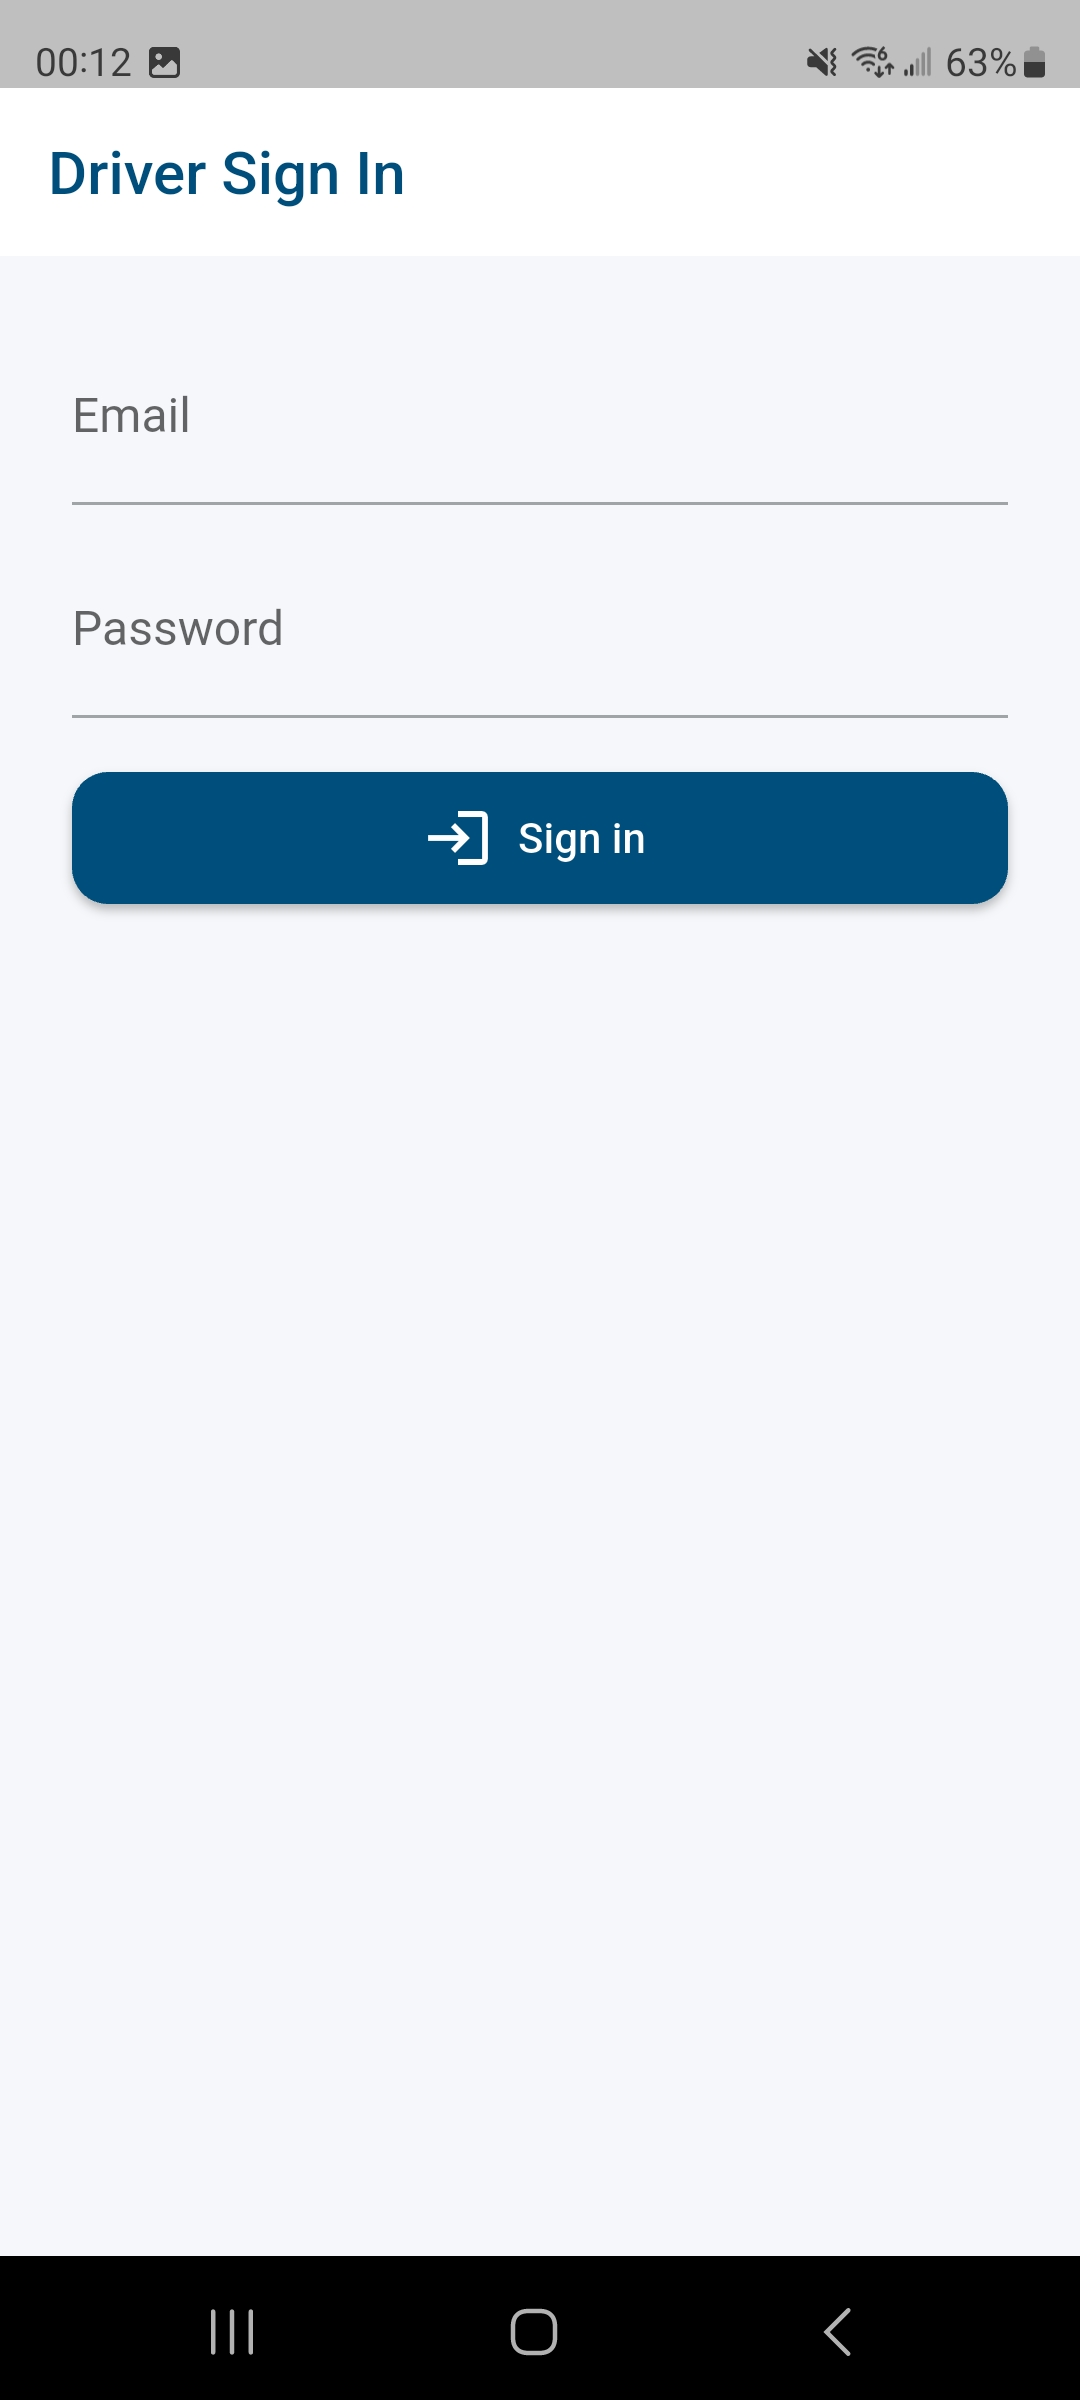
\includegraphics[width=0.45\textwidth]{ss-auth-login}
\caption{Login screen.}
\end{figure}

\begin{figure}[H]
\centering
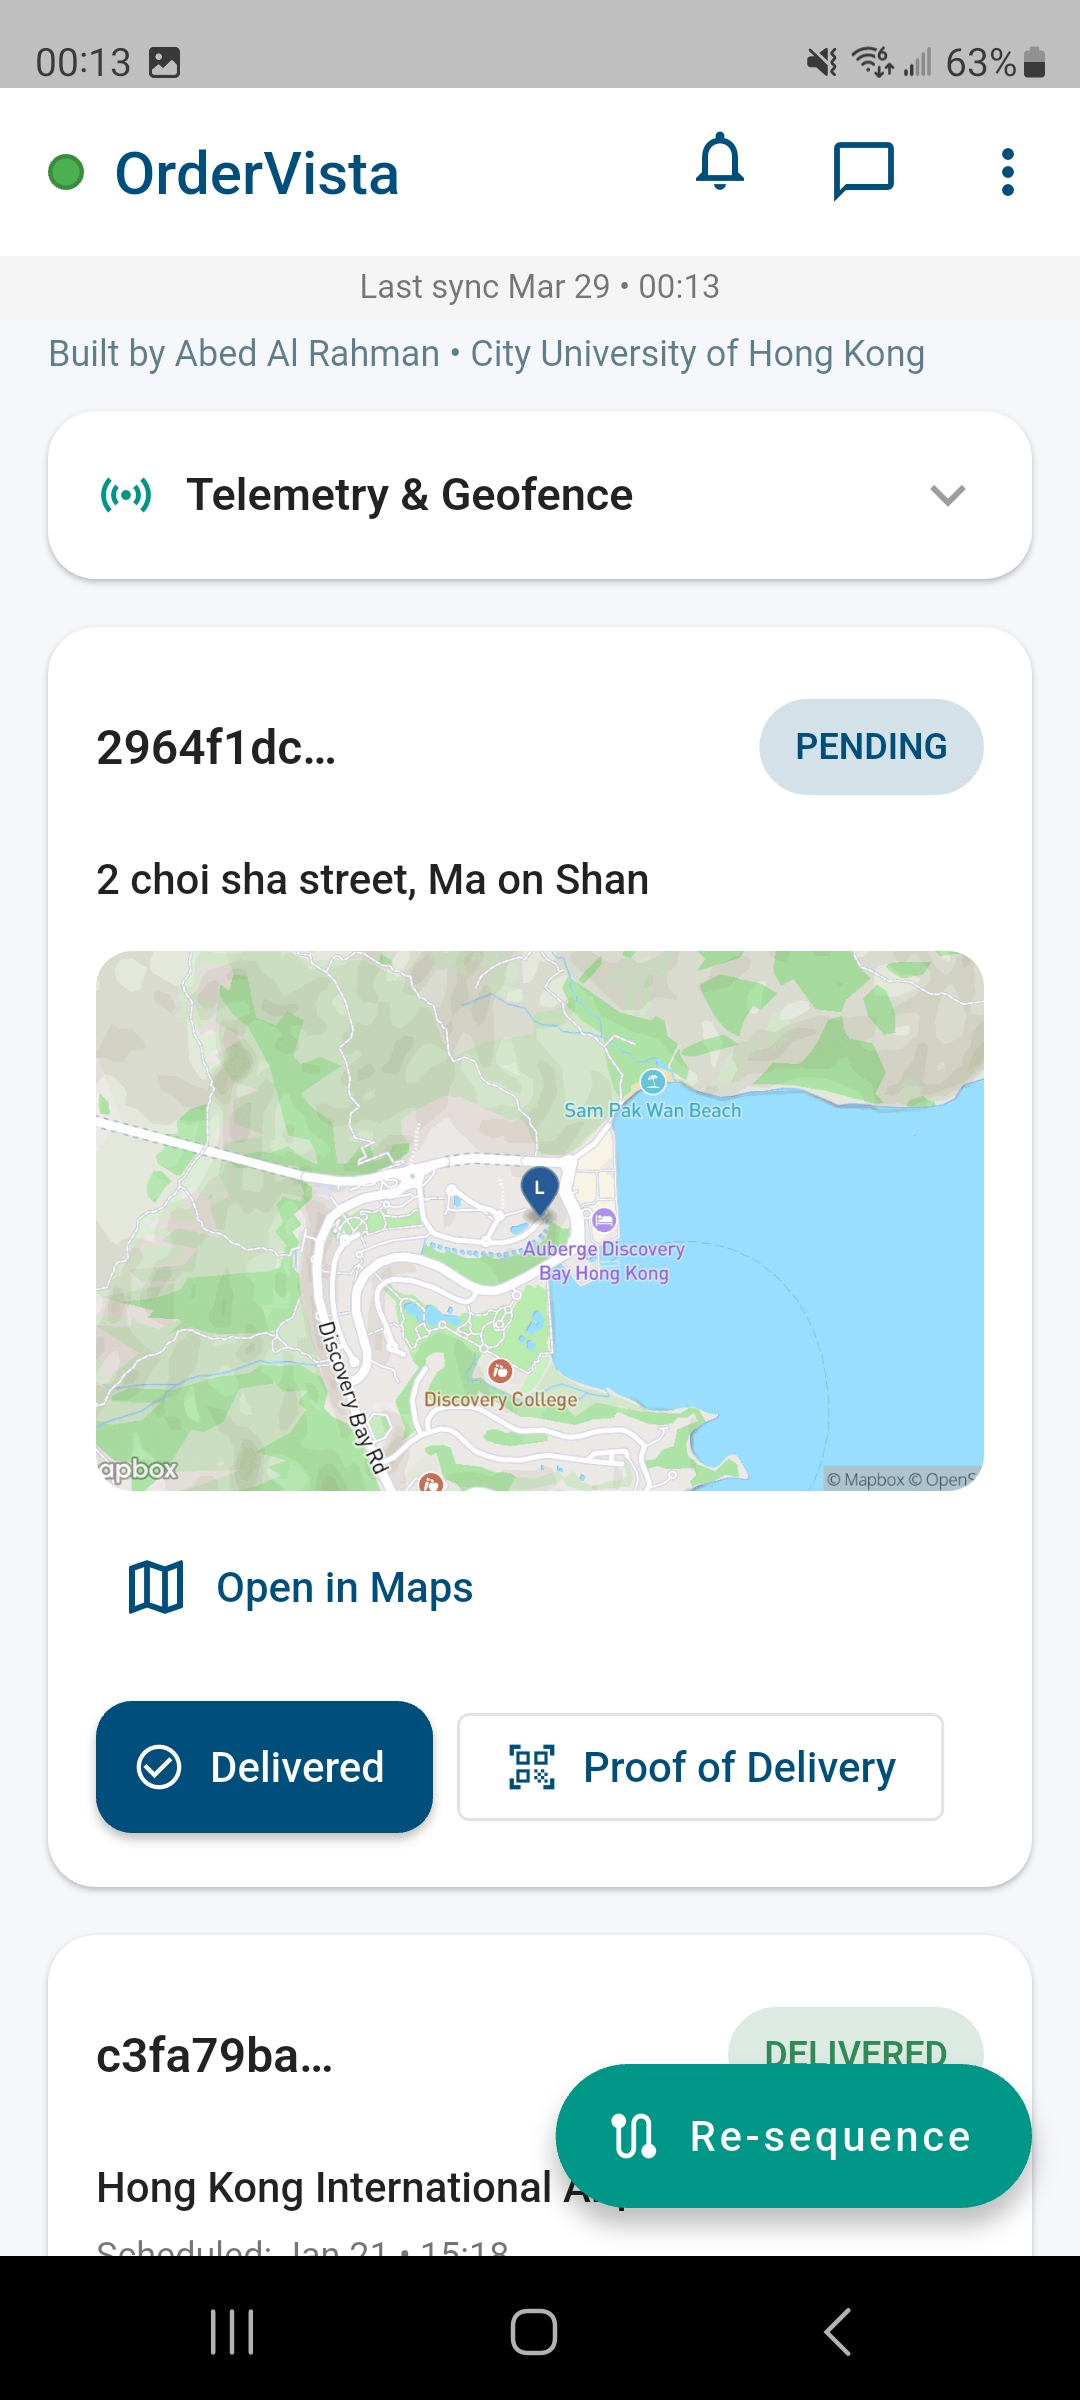
\includegraphics[width=0.45\textwidth]{ss-auth-redirect}
\caption{Role-based routing after authentication.}
\end{figure}

%--------------------------------------------------------------
\section{Admin Portal}

\begin{figure}[H]
\centering
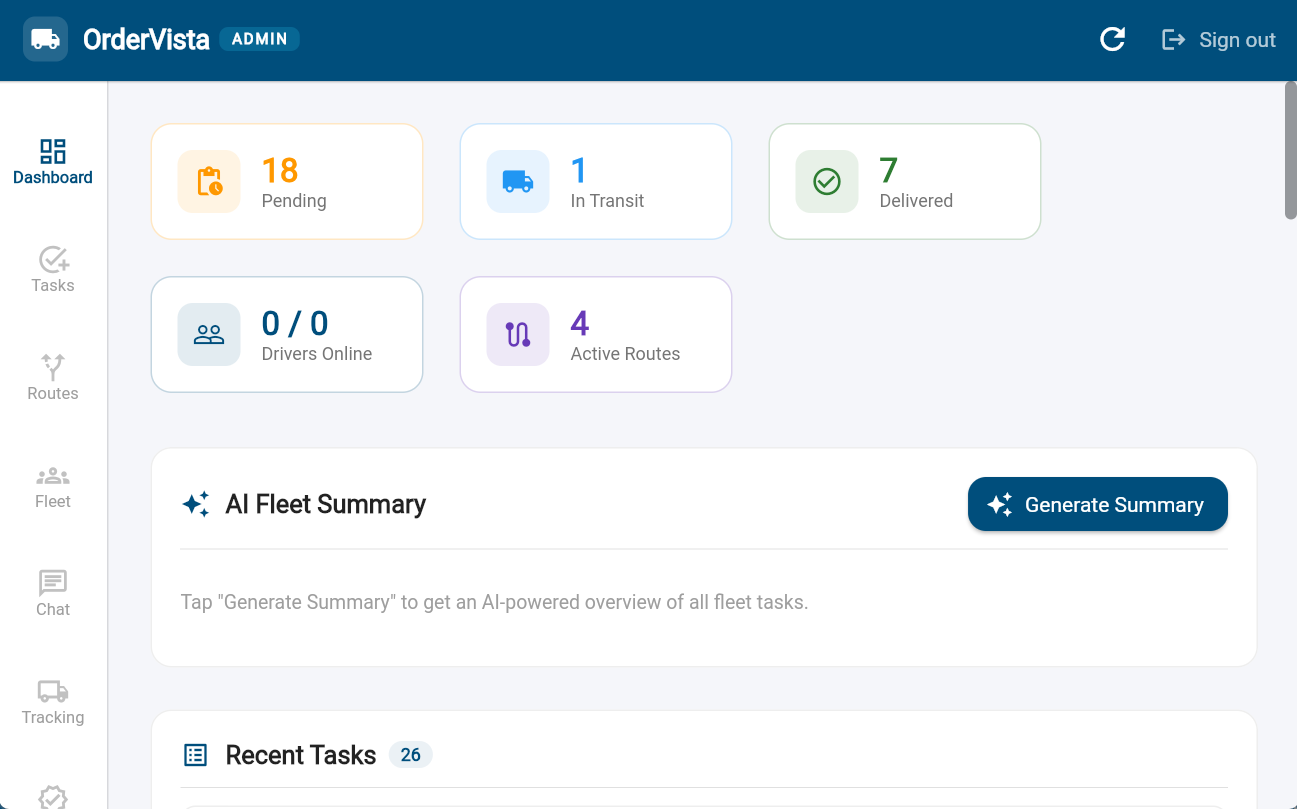
\includegraphics[width=0.7\textwidth]{ss-a1}
\caption{Admin dashboard overview.}
\end{figure}

\begin{figure}[H]
\centering
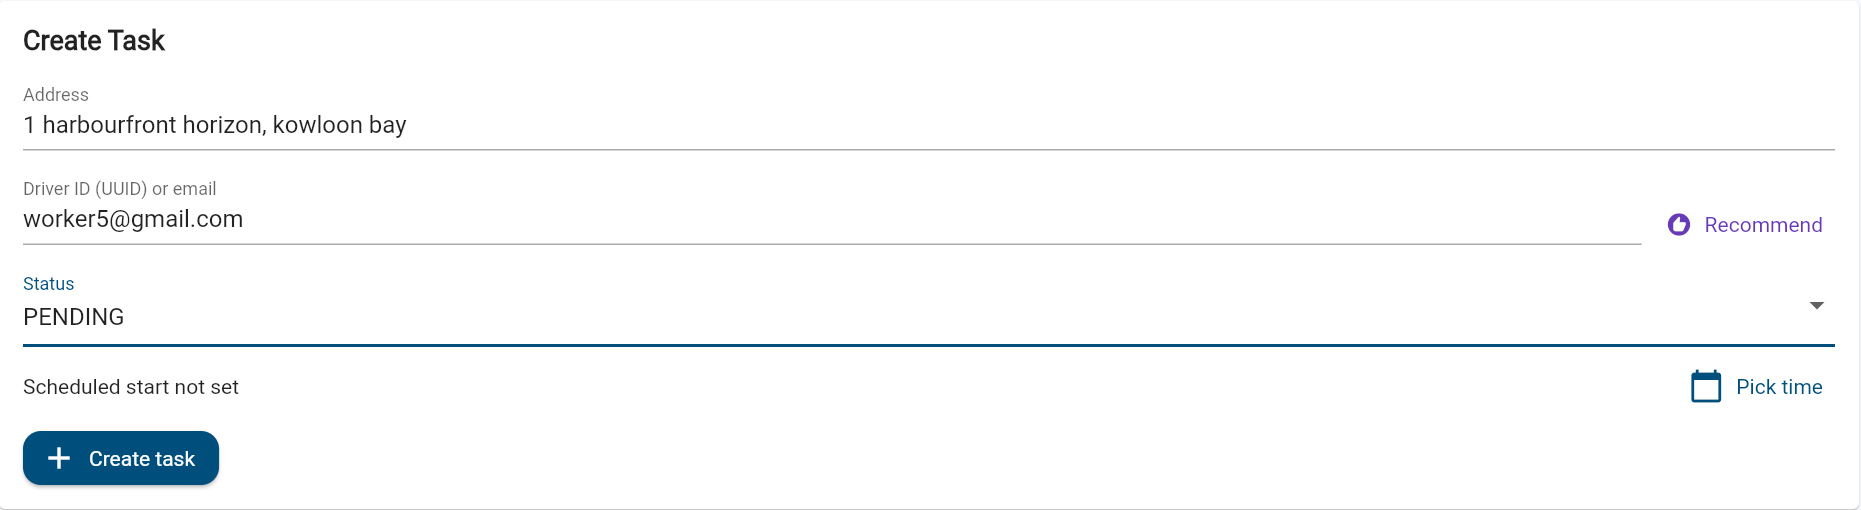
\includegraphics[width=0.7\textwidth]{ss-a2}
\caption{Task creation form.}
\end{figure}

\begin{figure}[H]
\centering
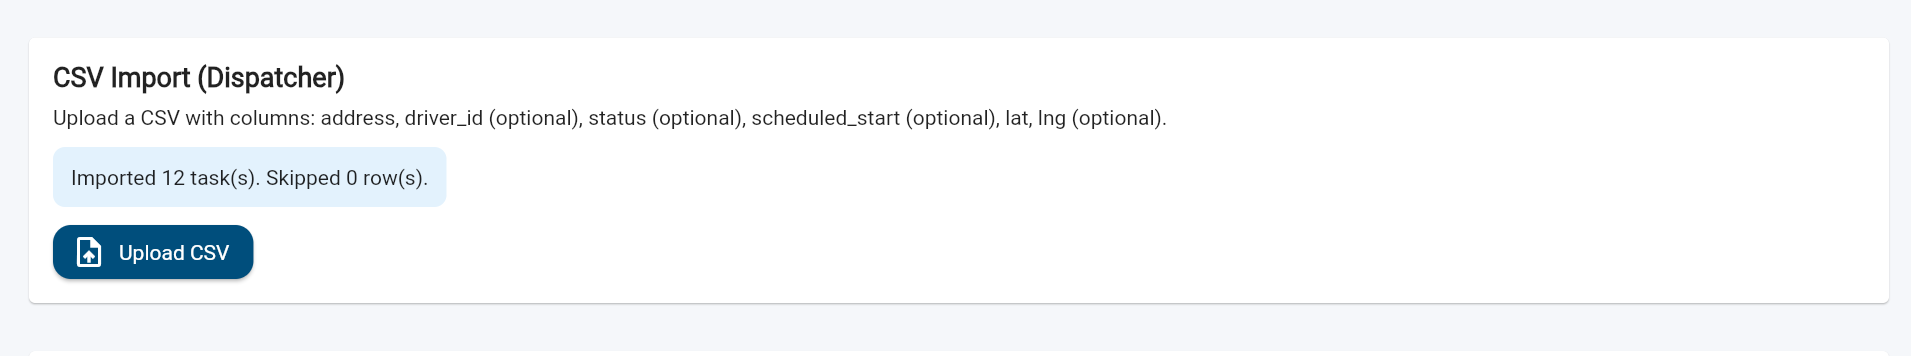
\includegraphics[width=0.7\textwidth]{ss-a3}
\caption{CSV bulk import with column mapping.}
\end{figure}

\begin{figure}[H]
\centering
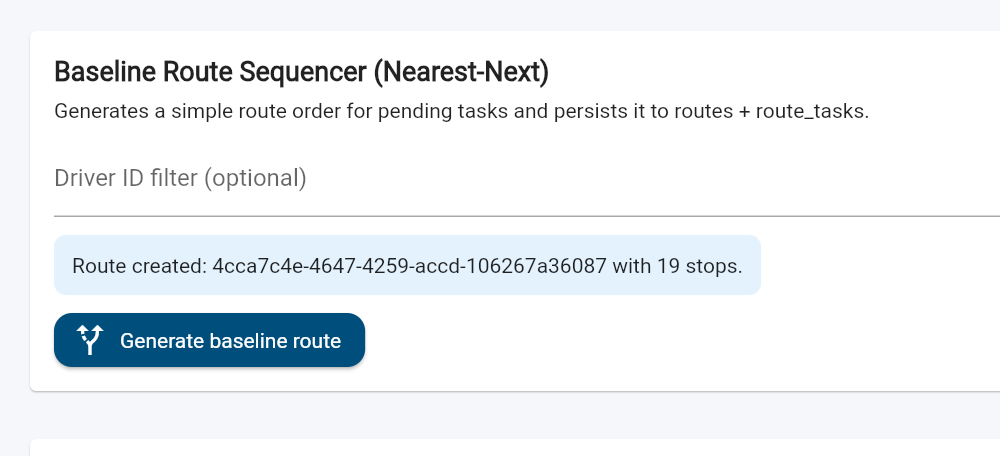
\includegraphics[width=0.7\textwidth]{ss-a6}
\caption{Route sequencing with static map preview.}
\end{figure}

\begin{figure}[H]
\centering
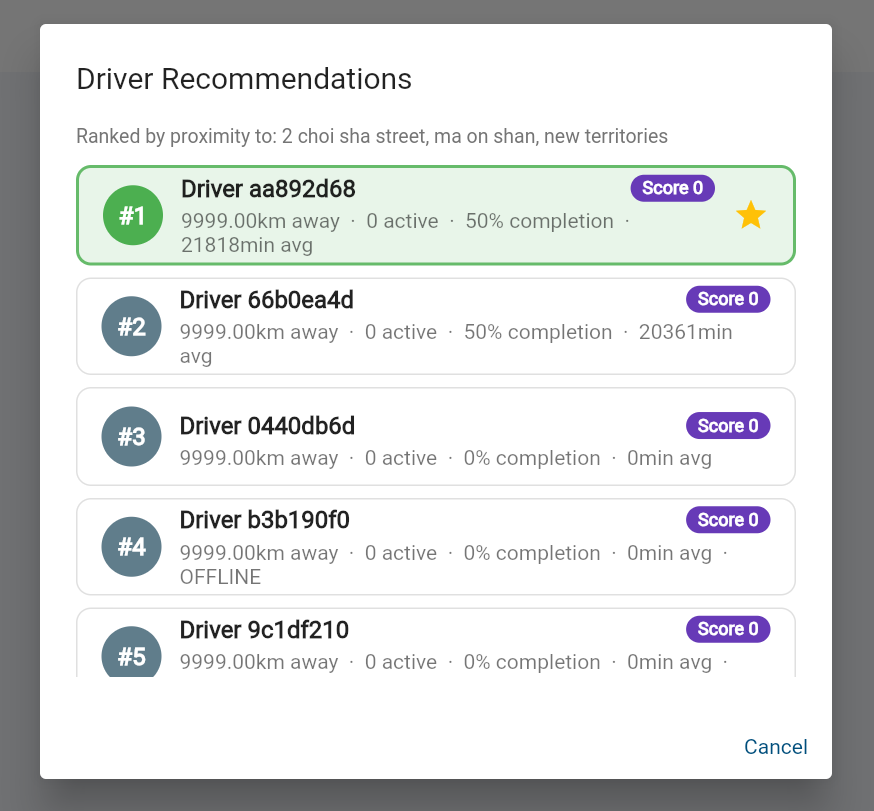
\includegraphics[width=0.7\textwidth]{ss-a7}
\caption{Driver recommendation panel.}
\end{figure}

\begin{figure}[H]
\centering
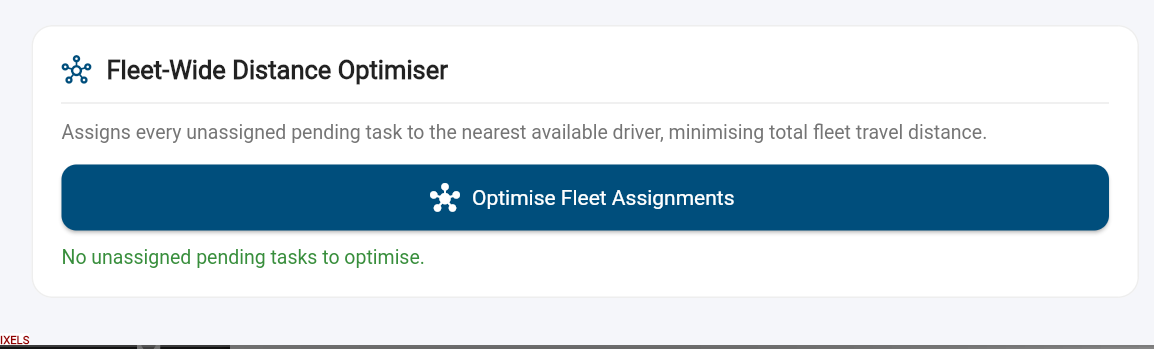
\includegraphics[width=0.7\textwidth]{ss-appd-fleet}
\caption{Fleet and vehicle management.}
\end{figure}

\begin{figure}[H]
\centering
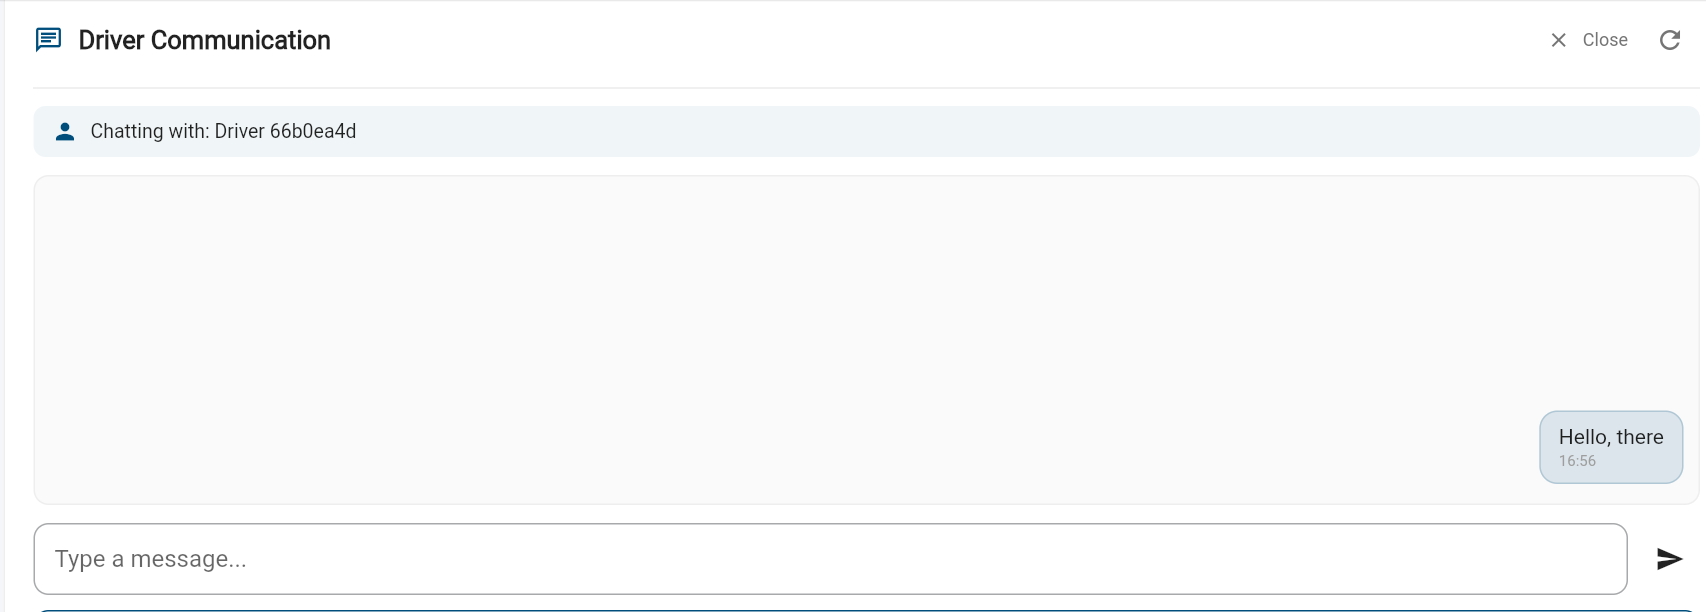
\includegraphics[width=0.7\textwidth]{ss-a10}
\caption{Admin--driver real-time chat.}
\end{figure}

\begin{figure}[H]
\centering
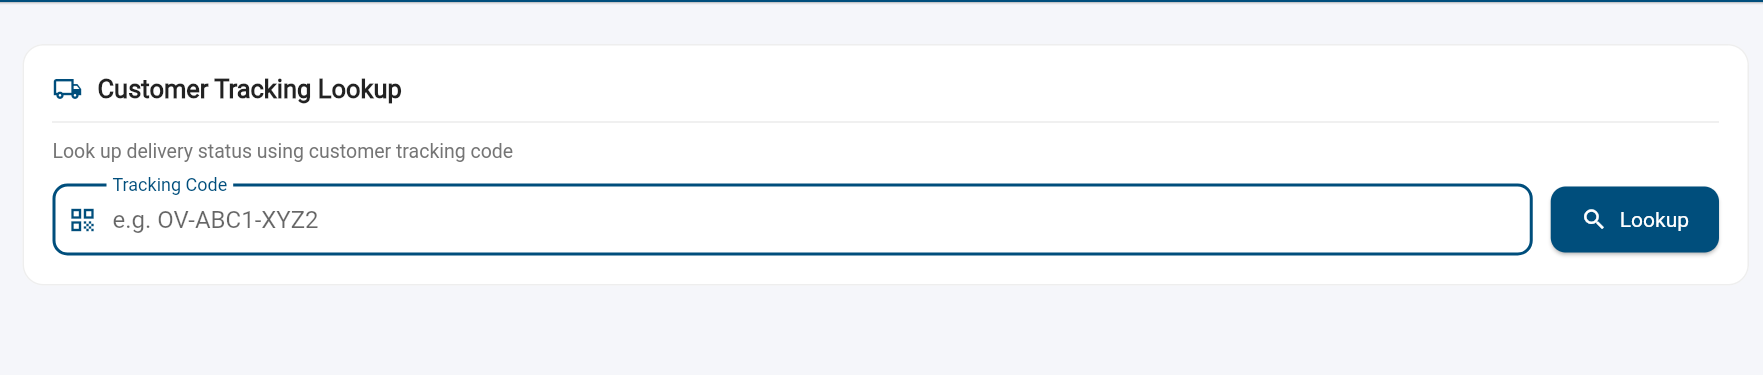
\includegraphics[width=0.7\textwidth]{ss-appd-tracking}
\caption{Customer delivery tracking.}
\end{figure}

%--------------------------------------------------------------
\section{Driver Application}

\begin{figure}[H]
\centering
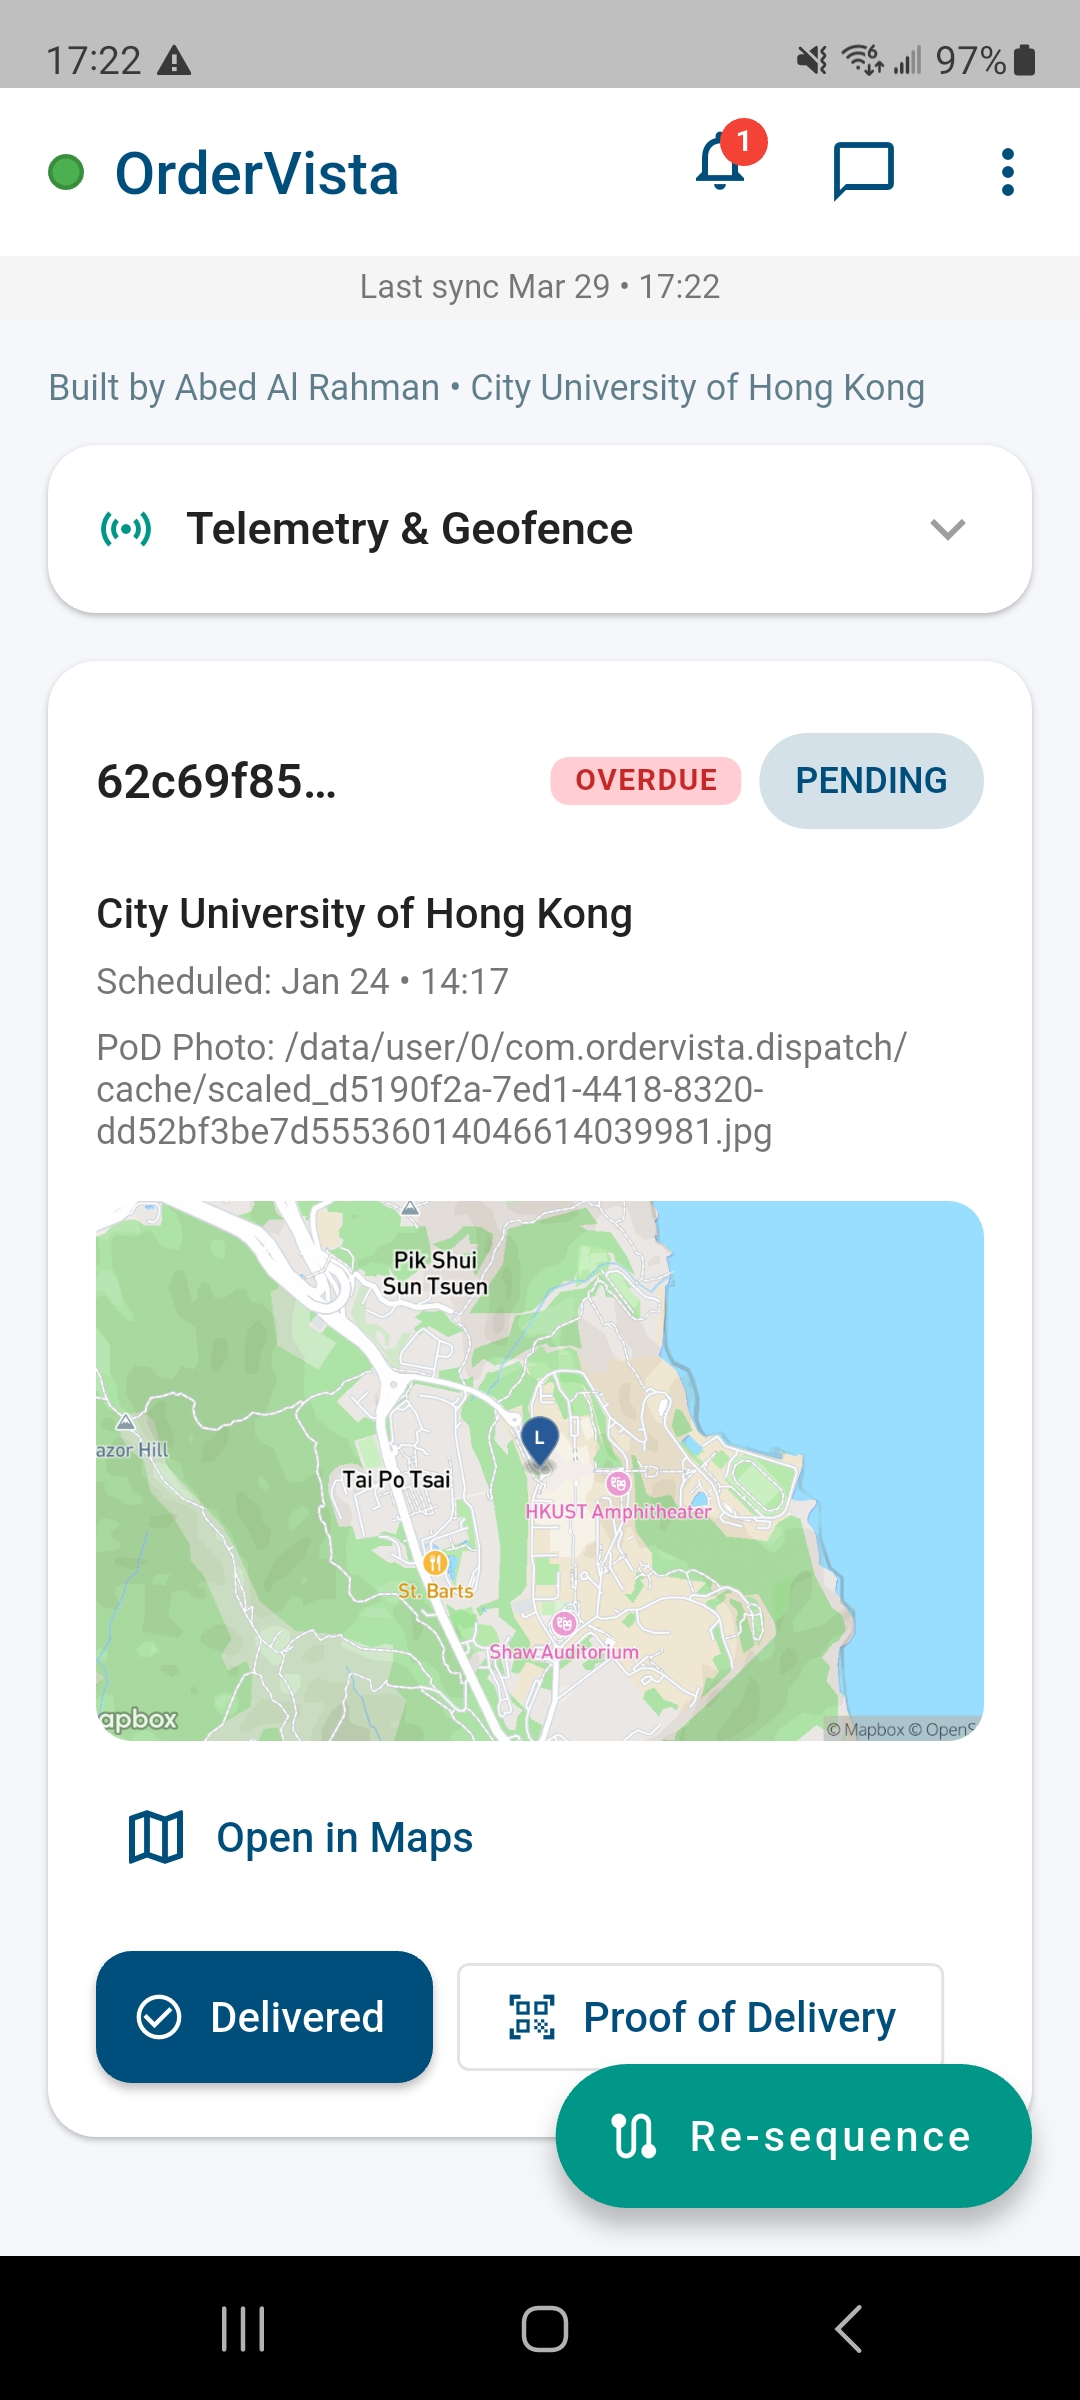
\includegraphics[width=0.45\textwidth]{ss-d1}
\caption{Driver task list.}
\end{figure}

\begin{figure}[H]
\centering
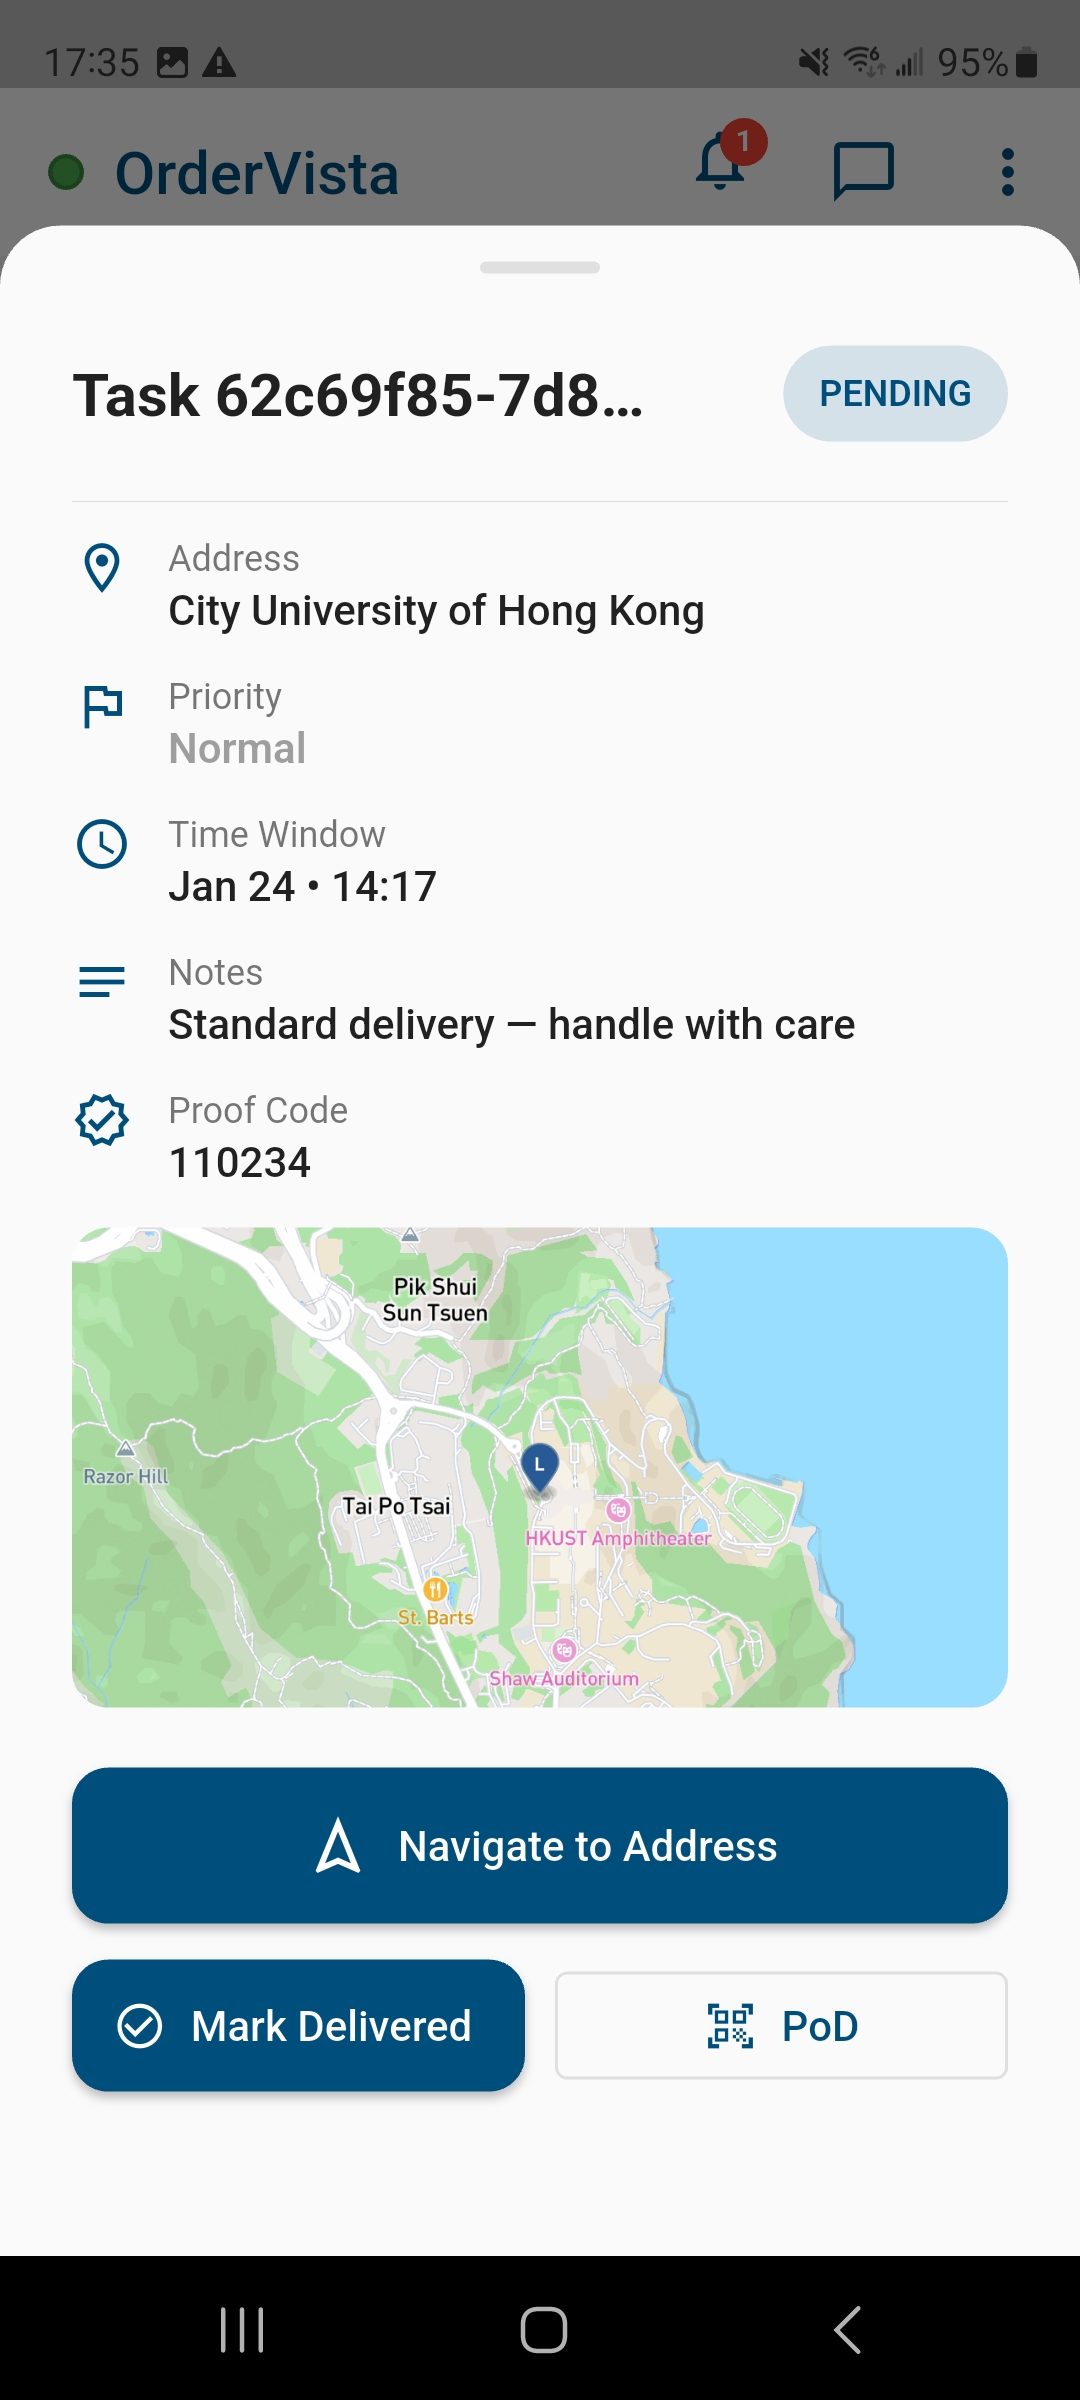
\includegraphics[width=0.45\textwidth]{ss-d2}
\caption{Task detail and navigation.}
\end{figure}

\begin{figure}[H]
\centering
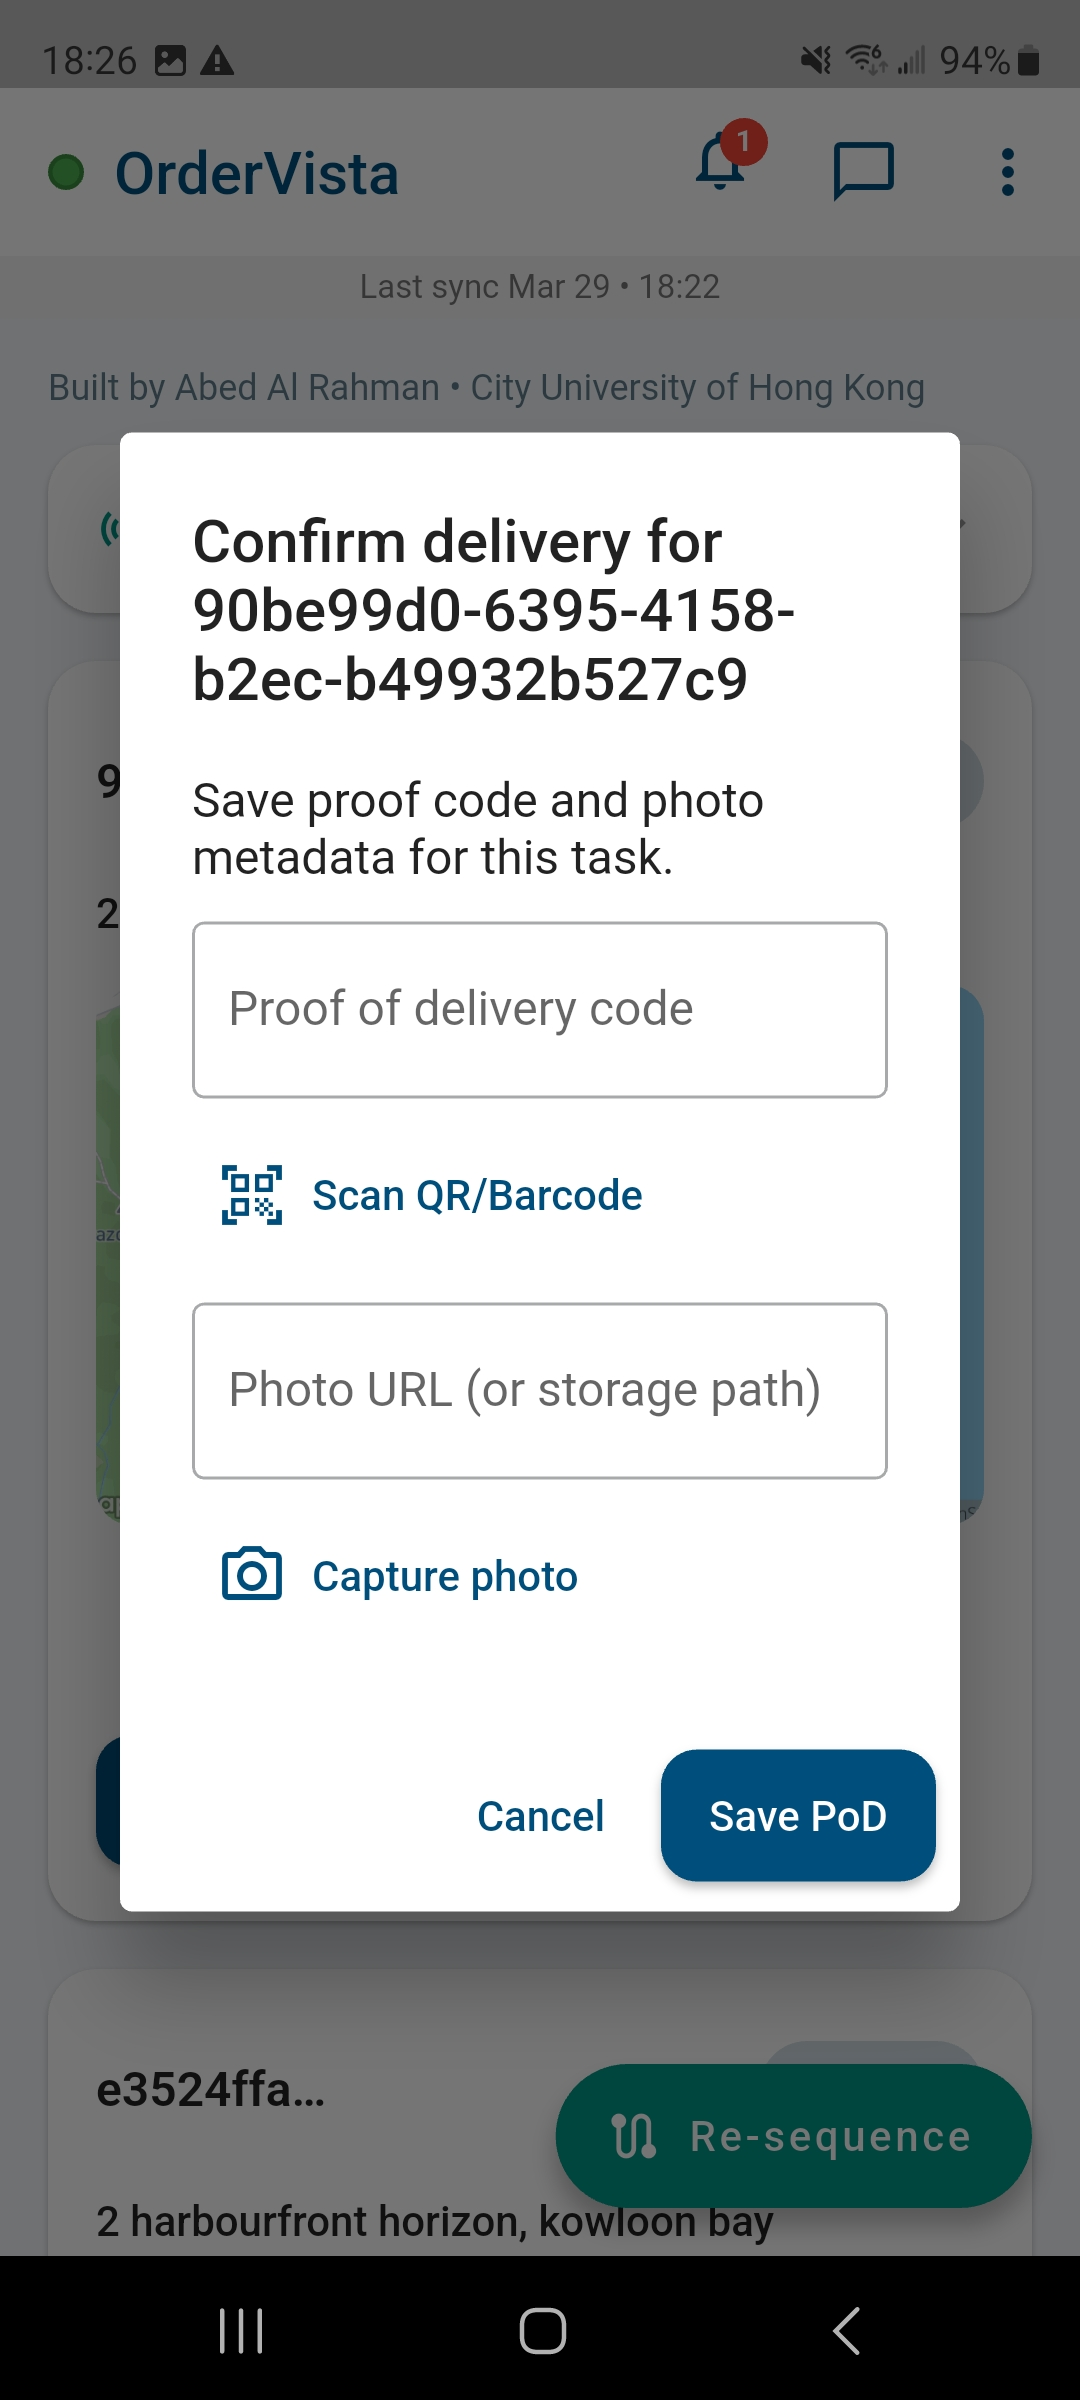
\includegraphics[width=0.45\textwidth]{ss-d4}
\caption{Proof of delivery capture.}
\end{figure}

\begin{figure}[H]
\centering
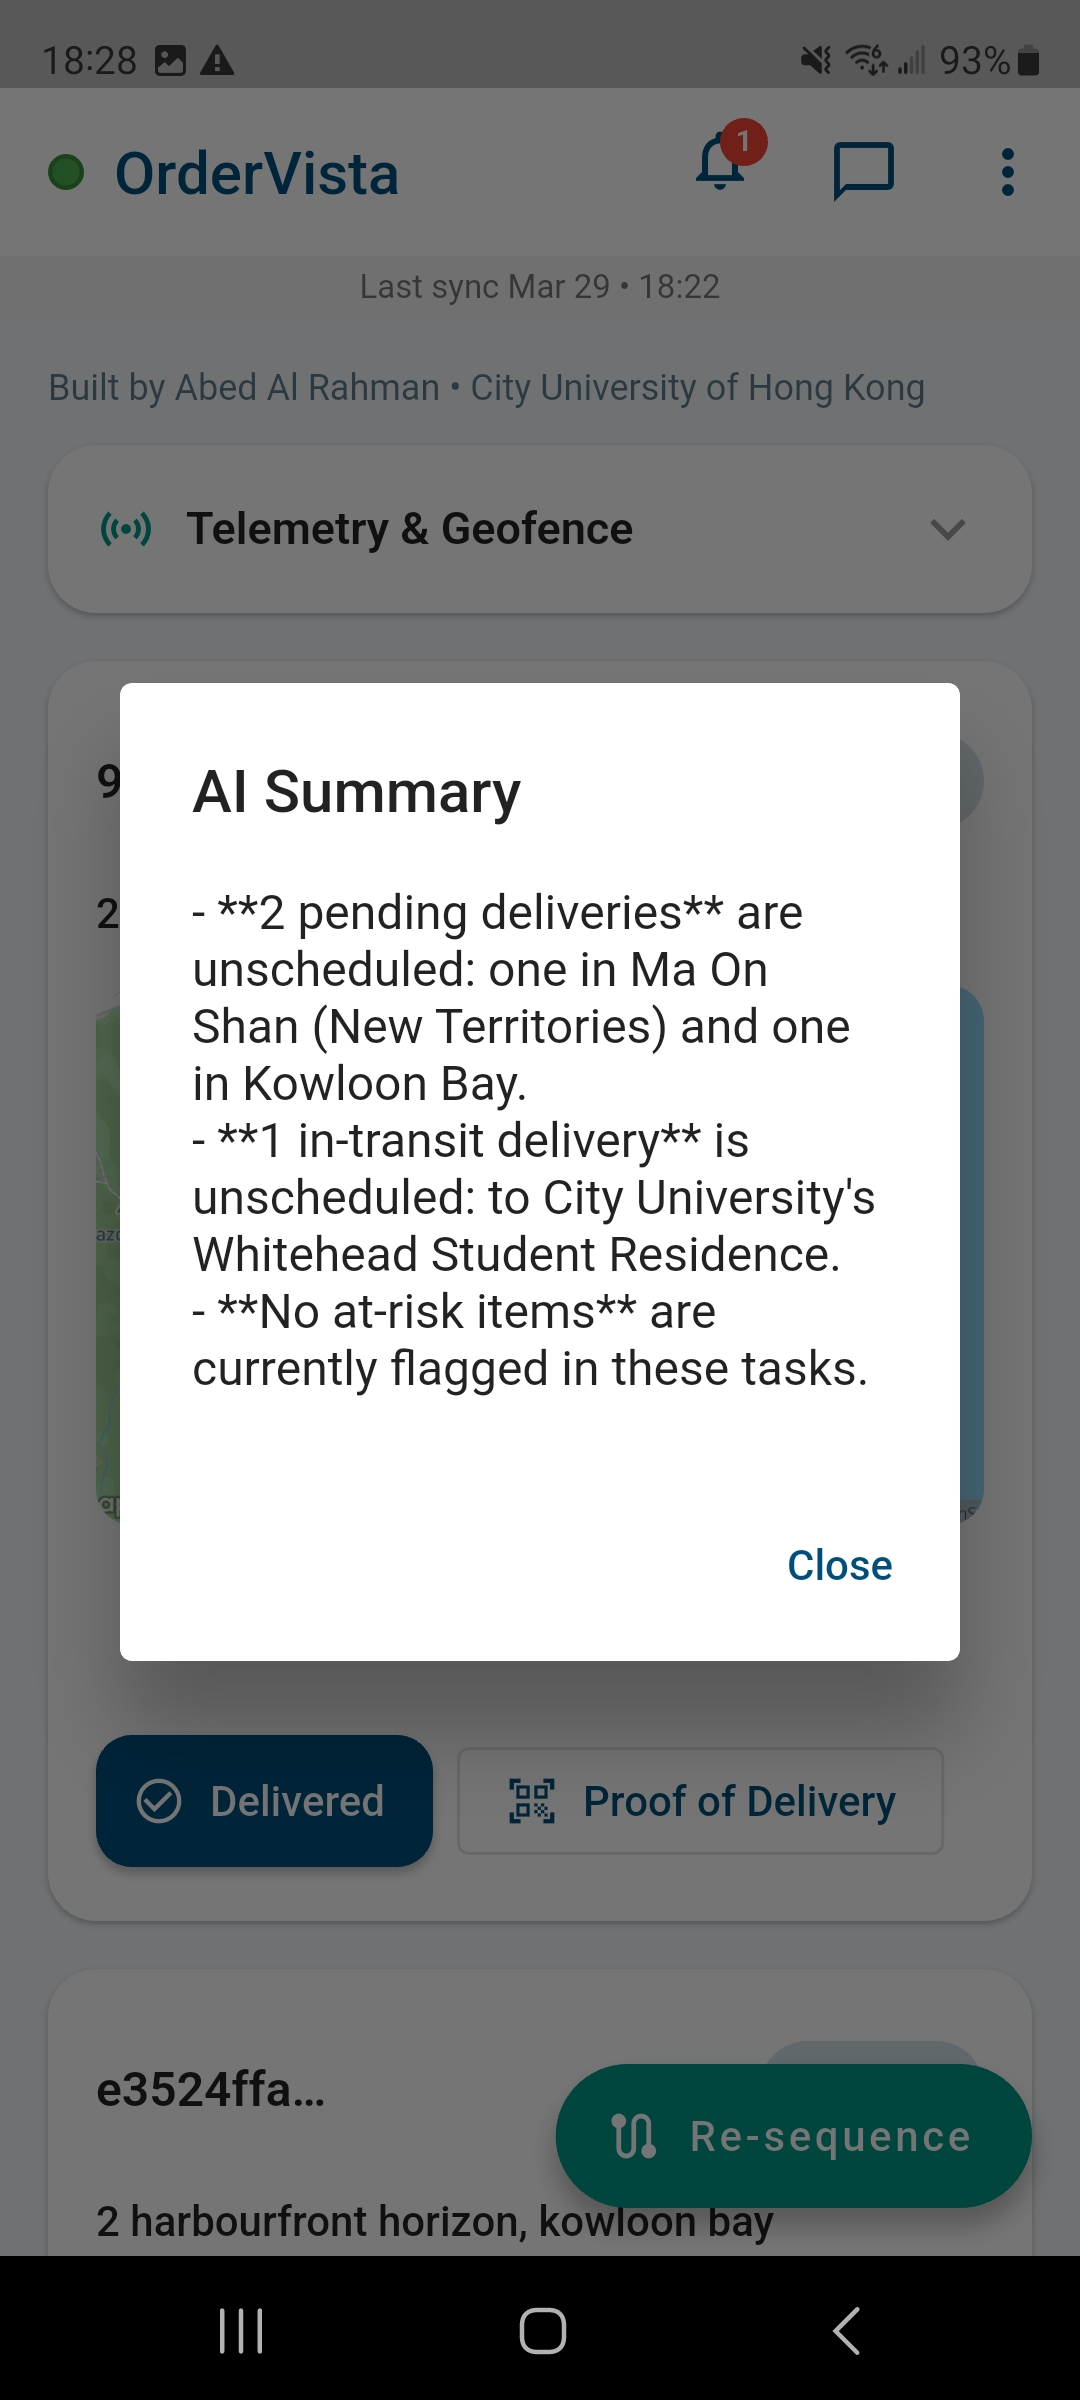
\includegraphics[width=0.45\textwidth]{ss-d6}
\caption{AI assistant: summary and chat.}
\end{figure}

\begin{figure}[H]
\centering
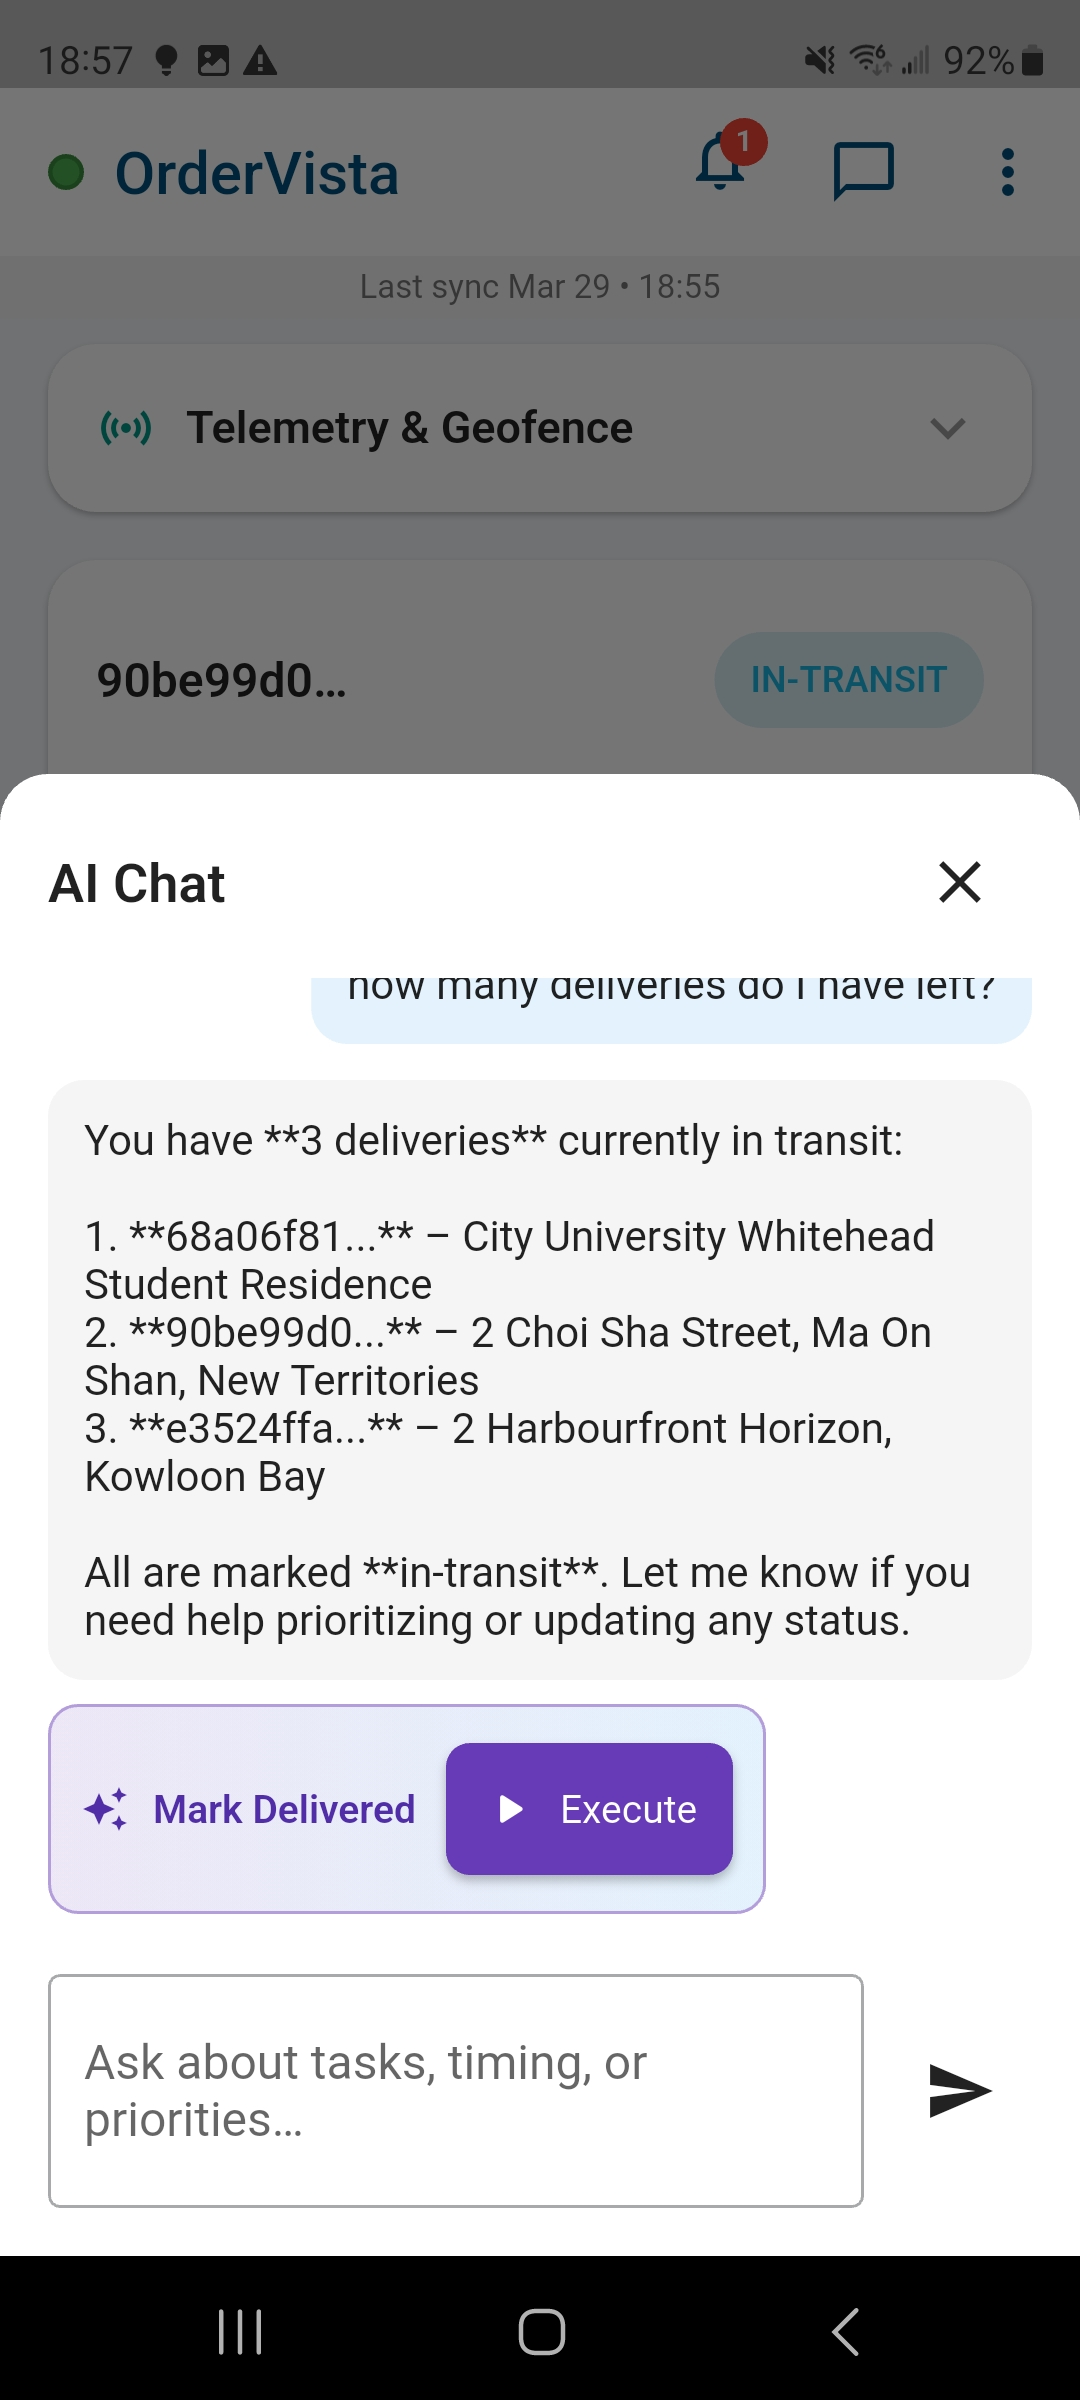
\includegraphics[width=0.45\textwidth]{ss-d8}
\caption{Agentic AI action with one-tap execution.}
\end{figure}

\begin{figure}[H]
\centering
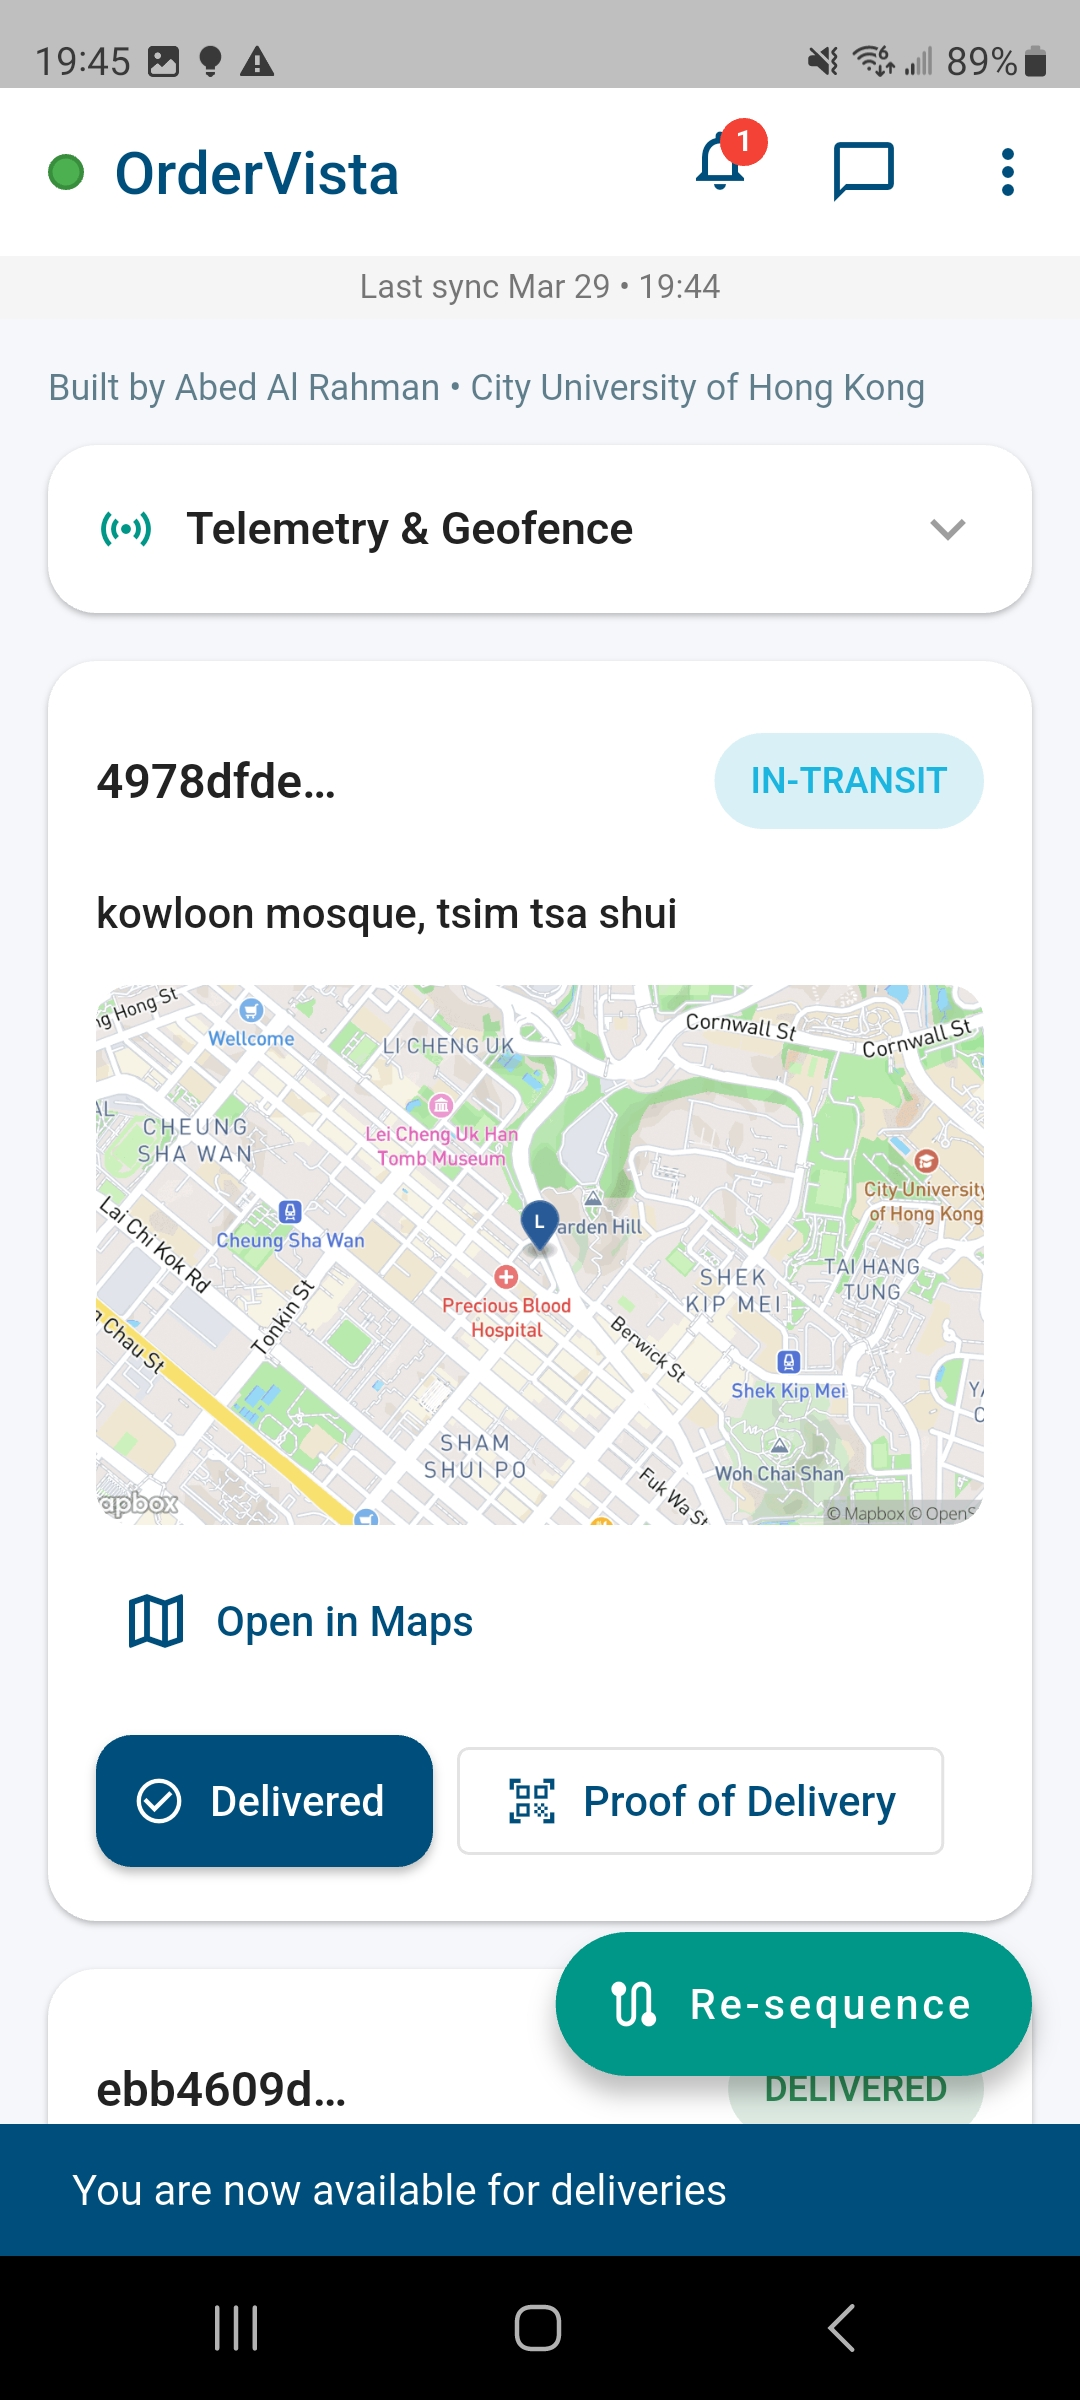
\includegraphics[width=0.45\textwidth]{ss-d13}
\caption{Driver telemetry panel.}
\end{figure}

\begin{figure}[H]
\centering
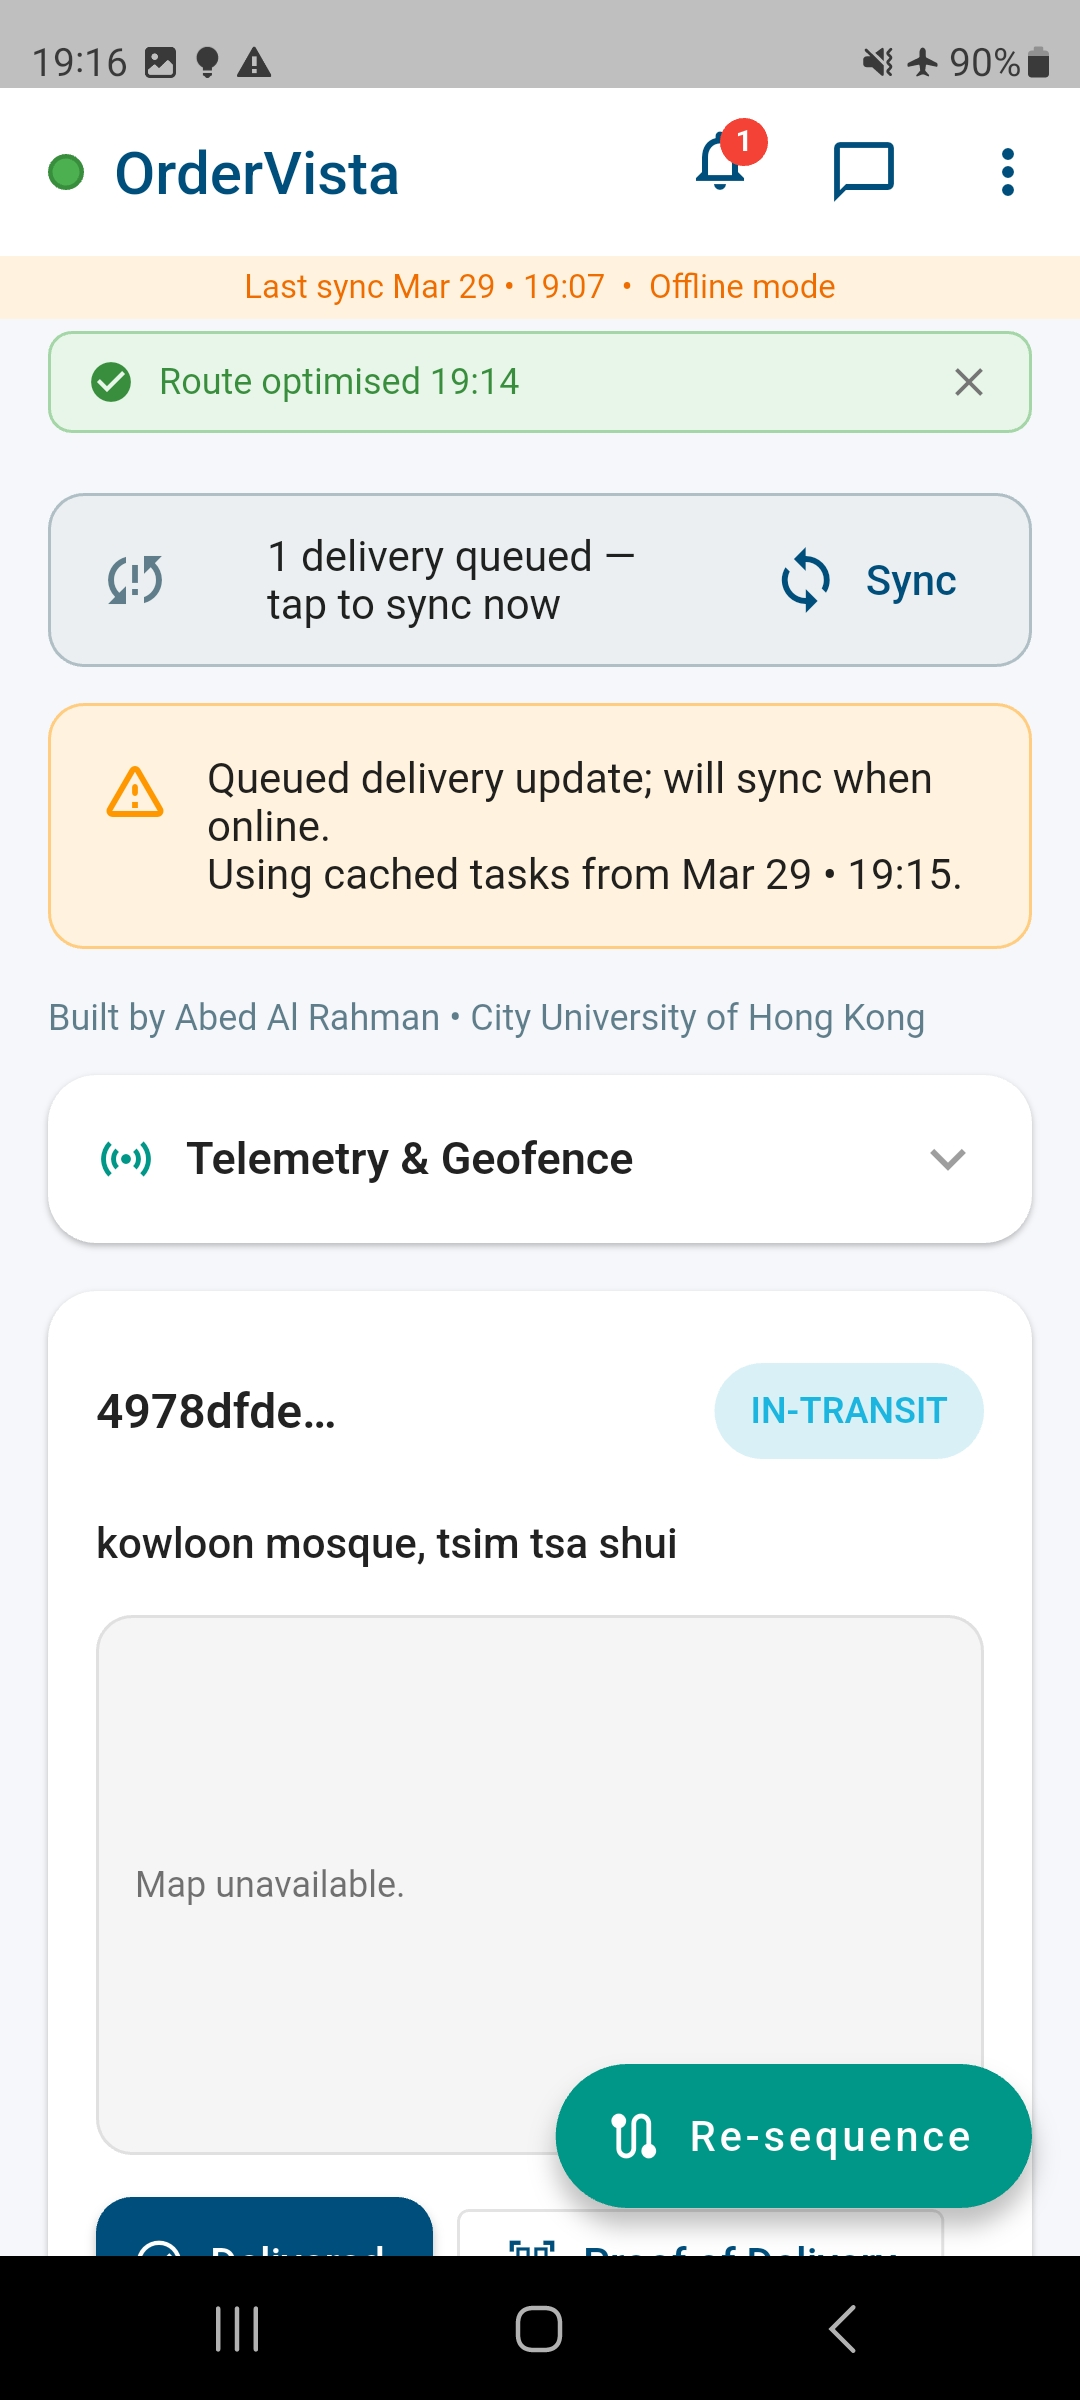
\includegraphics[width=0.45\textwidth]{ss-d11}
\caption{Offline mode with sync queue.}
\end{figure}

% Appendix E: Build and Deployment Evidence
\chapter{Build and Deployment Evidence}
\label{app:build}

This appendix documents the build configuration, dependency inventory, and
deployment artefacts produced for the OrderVista project.

%--------------------------------------------------------------
\section{Build Environment}

\begin{table}[H]
\centering
\caption{Build and development environment.}
\label{tab:build-env}
\begin{tabular}{@{}ll@{}}
\toprule
\textbf{Component} & \textbf{Version / Detail}\\
\midrule
Flutter SDK       & 3.35.2 (stable channel) \\
Dart SDK          & $\geq$\,3.0.0, $<$\,4.0.0 \\
Android Gradle Plugin & 8.9.1 \\
Kotlin            & 2.1.0 \\
Compile SDK       & 36 (Android 16) \\
Target SDK        & 35 (Android 15) \\
Min SDK           & 26 (Android 8.0 Oreo) \\
Java compatibility & 1.8 (desugared with \texttt{desugar\_jdk\_libs 2.1.4}) \\
Development OS    & Windows 10/11 \\
IDE               & Visual Studio Code with Flutter/Dart extensions \\
Version control   & Git + GitHub (branch-per-feature) \\
\bottomrule
\end{tabular}
\end{table}

%--------------------------------------------------------------
\section{Android Release Build}

The signed release APK was produced using the following command:

\begin{verbatim}
flutter build apk --release
\end{verbatim}

\begin{table}[H]
\centering
\caption{Release APK details.}
\label{tab:release-apk}
\begin{tabular}{@{}ll@{}}
\toprule
\textbf{Property} & \textbf{Value}\\
\midrule
Application ID    & \texttt{com.ordervista.dispatch} \\
Version name      & 1.0.0 \\
Version code      & 1 \\
APK size          & 75.7\,MB \\
Signing           & Release keystore (SHA-256 signed) \\
ProGuard          & Enabled (default rules) \\
\bottomrule
\end{tabular}
\end{table}

\begin{figure}[H]
\centering
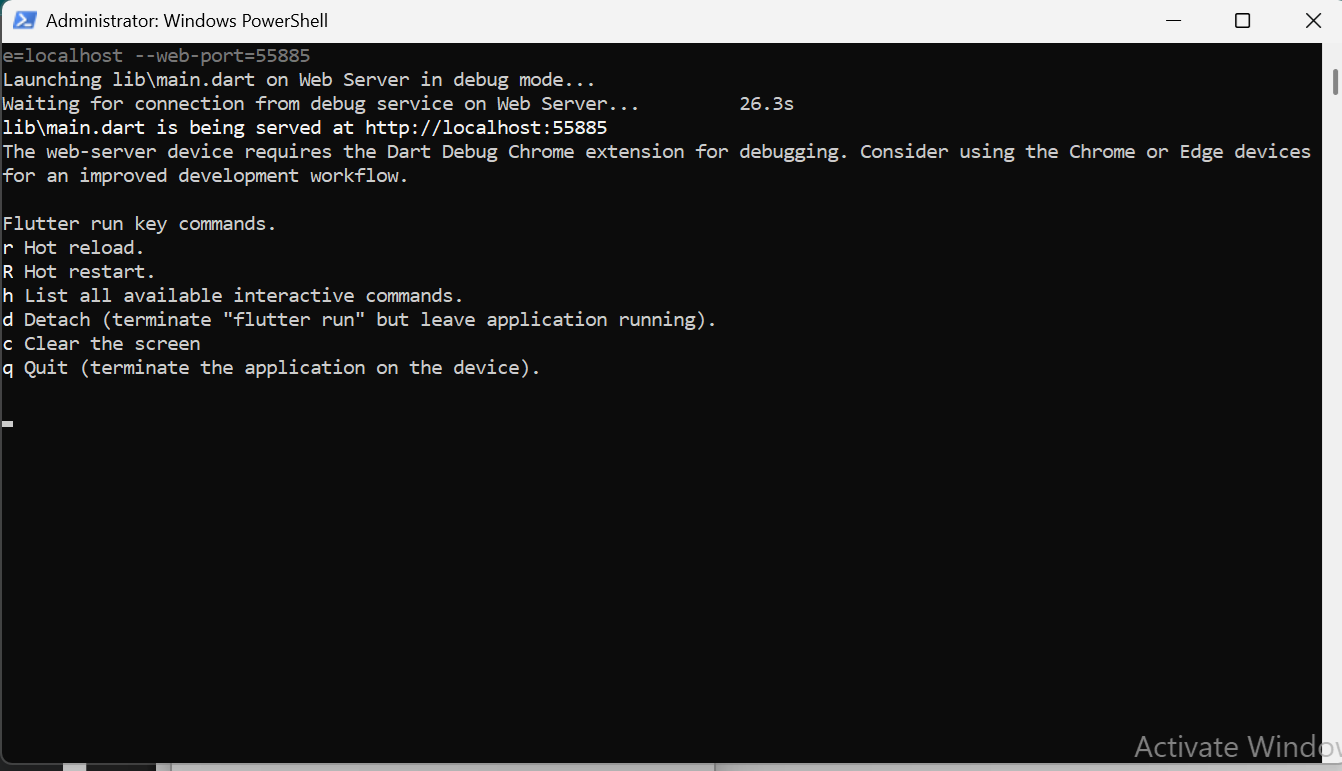
\includegraphics[width=0.7\textwidth]{ss-build-output}
\caption{Terminal output of a successful \texttt{flutter build apk --release}.}
\label{fig:build-output}
\end{figure}

%--------------------------------------------------------------
\section{Backend Deployment}

\begin{table}[H]
\centering
\caption{Supabase project configuration.}
\label{tab:supabase-config}
\begin{tabular}{@{}ll@{}}
\toprule
\textbf{Setting} & \textbf{Value}\\
\midrule
Hosting          & Supabase Cloud (free tier) \\
Region           & Southeast Asia \\
PostgreSQL       & 15.x with PostGIS extension \\
Authentication   & Supabase Auth (email/password) \\
Storage          & Supabase Storage (PoD photos) \\
Realtime         & Enabled for \texttt{chat\_messages} and \texttt{tasks} \\
Migrations       & 3 SQL migration files (see Appendix~\ref{app:schema}) \\
\bottomrule
\end{tabular}
\end{table}

%--------------------------------------------------------------
\section{External Service Configuration}

\begin{table}[H]
\centering
\caption{External API integrations.}
\label{tab:ext-apis}
\begin{tabular}{@{}lll@{}}
\toprule
\textbf{Service} & \textbf{Purpose} & \textbf{Plan}\\
\midrule
Mapbox Geocoding API   & Address $\to$ coordinates & Free tier \\
Mapbox Static Images   & Route map previews       & Free tier \\
OpenRouter API         & LLM gateway              & Pay-per-token \\
DeepSeek R1            & AI model (via OpenRouter) & Free tier \\
\bottomrule
\end{tabular}
\end{table}

%--------------------------------------------------------------
\section{Dependency Inventory}

Table~\ref{tab:deps} lists the principal Dart/Flutter packages used.

\begin{small}
\begin{longtable}{@{}llp{7cm}@{}}
\caption{Key project dependencies.}
\label{tab:deps}\\
\toprule
\textbf{Package} & \textbf{Version} & \textbf{Purpose}\\
\midrule
\endfirsthead
\toprule
\textbf{Package} & \textbf{Version} & \textbf{Purpose}\\
\midrule
\endhead
\bottomrule
\endlastfoot

\texttt{supabase\_flutter}    & 2.3.4  & Supabase client (auth, DB, storage, realtime) \\
\texttt{drift}                & 2.18.0 & SQLite ORM for offline cache \\
\texttt{sqlite3\_flutter\_libs} & 0.5.22 & Native SQLite bindings \\
\texttt{go\_router}           & 12.1.3 & Declarative routing with role guards \\
\texttt{provider}             & 6.1.5  & State management (ChangeNotifier) \\
\texttt{geolocator}           & 11.0.0 & GPS location services \\
\texttt{mobile\_scanner}      & 4.0.1  & Barcode and QR code scanning \\
\texttt{image\_picker}        & 1.1.2  & Camera photo capture \\
\texttt{csv}                  & 6.0.0  & CSV parsing for bulk import \\
\texttt{file\_picker}         & 10.3.8 & File selection dialog \\
\texttt{cached\_network\_image} & 3.4.1 & Image caching with placeholders \\
\texttt{google\_fonts}        & 6.1.0  & Typography \\
\texttt{flutter\_animate}     & 4.5.0  & Declarative animations \\
\texttt{intl}                 & 0.20.2 & Date/number formatting \\
\texttt{timeago}              & 3.7.1  & Relative time display \\
\texttt{url\_launcher}        & 6.3.1  & External link/map navigation \\
\texttt{shared\_preferences}  & 2.5.3  & Key-value persistent storage \\
\texttt{json\_path}           & 0.7.2  & JSON querying for AI responses \\
\end{longtable}
\end{small}

%--------------------------------------------------------------
\section{Repository Structure}

\begin{verbatim}
ordervista/
  lib/
    main.dart               # Entry point
    app/                    # App shell, theme, router
    bootstrap/              # Initialisation, DI
    config/                 # AppConfig, environment
    data/                   # Drift database, DAOs
    models/                 # Domain models
    repositories/           # Repository pattern layer
    services/               # Supabase, Mapbox, AI services
    viewmodels/             # MVVM view-models
    screens/                # Admin portal screens
    pages/                  # Driver app pages
    components/             # Shared UI components
  supabase/
    migrations/             # 3 SQL migration files
  android/                  # Android build config
  test/                     # Unit and widget tests
  pubspec.yaml              # Dependencies
\end{verbatim}

%--------------------------------------------------------------
\section{Web Deployment}
\label{sec:web-deploy}

The admin portal is deployed as a Flutter Web release on Vercel.
The production URL is:

\begin{center}
\url{https://ordervista.vercel.app}
\end{center}

The web build was compiled with environment variables baked in at build time
using \texttt{flutter build web --release --dart-define-from-file=.env}.
A \texttt{vercel.json} rewrite rule ensures that Flutter's client-side
routing functions correctly on page refresh and deep links.

%--------------------------------------------------------------
\section{Google Play Store Submission}
\label{sec:play-store}

A signed Android App Bundle (\texttt{app-release.aab}, 55.9\,MB) was uploaded
to Google Play Console under the closed testing track.  At the time of
writing, 12~testers have been recruited and the mandatory 14-day closed
testing period required by Google for new developer accounts is in progress.
Production access will be requested upon completion of this review period.

%--------------------------------------------------------------
\section{Evaluation Access Credentials}
\label{sec:eval-creds}

Table~\ref{tab:eval-creds} provides test credentials for evaluators to
access the live deployment.  These accounts are provisioned on the project's
Supabase instance and are intended solely for examination purposes.

\begin{table}[H]
\centering
\caption{Evaluation credentials for the live system.}
\label{tab:eval-creds}
\begin{tabular}{@{}llll@{}}
\toprule
\textbf{Role} & \textbf{Email} & \textbf{Password} & \textbf{Access Point}\\
\midrule
Admin / Dispatcher & \texttt{abed-al-rahman@cityu.com} & \texttt{profgerhardcs4514} & \url{https://ordervista.vercel.app} \\
Driver             & \texttt{worker2@gmail.com}          & \texttt{worker2}          & Android APK \\
Driver             & \texttt{worker3@gmail.com}          & \texttt{worker3}          & Android APK \\
Driver             & \texttt{worker4@gmail.com}          & \texttt{worker4}          & Android APK \\
Driver             & \texttt{worker5@gmail.com}          & \texttt{worker5}          & Android APK \\
\bottomrule
\end{tabular}
\end{table}

\noindent\textbf{Note:} The admin portal is accessible via web browser.  The
driver application requires the signed Android APK installed on a physical
device (GPS and camera features are not available in browser).

% Appendix F: Extended Test Cases
\chapter{Extended Test Cases}
\label{app:testcases}

This appendix provides the detailed test procedures that supplement the
summary tables in Chapter~\ref{ch:testing}.  Each case specifies
preconditions, step-by-step actions, and the expected versus observed
outcome.

%--------------------------------------------------------------
\section{Admin Functional Tests}

\begin{longtable}{@{}p{1.0cm}p{2.4cm}p{4.2cm}p{3.2cm}p{2.0cm}@{}}
\caption{Extended admin test procedures.}
\label{tab:ext-admin}\\
\toprule
\textbf{ID} & \textbf{Test} & \textbf{Steps} & \textbf{Expected Result} & \textbf{Status}\\
\midrule
\endfirsthead
\toprule
\textbf{ID} & \textbf{Test} & \textbf{Steps} & \textbf{Expected Result} & \textbf{Status}\\
\midrule
\endhead
\midrule \multicolumn{5}{r}{\textit{Continued on next page}}\\
\endfoot
\bottomrule
\endlastfoot

A1 & Admin login &
  1.~Open app.\newline
  2.~Enter admin email and password.\newline
  3.~Tap ``Sign In''. &
  Dashboard loads; navigation shows admin menu items. &
  \checkmark\\

A2 & Create single task &
  1.~Navigate to Tasks.\newline
  2.~Tap ``+ New Task''.\newline
  3.~Enter address; wait for geocode.\newline
  4.~Assign driver; set schedule.\newline
  5.~Save. &
  Task appears in list with ``pending'' status and geocoded coordinates. &
  \checkmark\\

A3 & Edit existing task &
  1.~Tap a pending task.\newline
  2.~Change address and priority.\newline
  3.~Save. &
  Updated fields persist on reload; \texttt{updated\_at} timestamp refreshed. &
  \checkmark\\

A4 & Delete task &
  1.~Tap a pending task.\newline
  2.~Tap ``Delete''.\newline
  3.~Confirm. &
  Task removed from list and database. &
  \checkmark\\

A5 & CSV bulk import &
  1.~Navigate to Import.\newline
  2.~Select a CSV file (10+ rows).\newline
  3.~Map columns.\newline
  4.~Tap ``Import''. &
  All rows geocoded and inserted; progress indicator completes; task count increases. &
  \checkmark\\

A6 & Generate optimised route &
  1.~Select 5+ unassigned tasks.\newline
  2.~Tap ``Generate Route''.\newline
  3.~Review map preview. &
  Route created with numbered stops in NN order; static map displays pins. &
  \checkmark\\

A7 & Assign driver to route &
  1.~Open generated route.\newline
  2.~Select a driver.\newline
  3.~Confirm assignment. &
  Route status changes to ``assigned''; driver sees tasks on their device. &
  \checkmark\\

A8 & Driver recommendation &
  1.~Open a task or route.\newline
  2.~Tap ``Recommend Driver''. &
  Ranked list of drivers with availability, distance, completion rate, and composite score. &
  \checkmark\\

A9 & Review PoD &
  1.~Navigate to a delivered task.\newline
  2.~View proof panel. &
  Photo thumbnail and confirmation code visible; timestamp matches driver submission. &
  \checkmark\\

A10 & Send chat message &
  1.~Open Chat.\newline
  2.~Select a driver.\newline
  3.~Type and send message. &
  Message appears in conversation; driver receives it in real time. &
  \checkmark\\

A11 & Broadcast message &
  1.~Open Chat.\newline
  2.~Tap ``Broadcast''.\newline
  3.~Type and send. &
  All drivers within the company see the broadcast. &
  \checkmark\\

A12 & AI fleet summary &
  1.~Navigate to AI tab.\newline
  2.~Tap ``Generate Summary''. &
  DeepSeek returns a structured summary of today's fleet activity. &
  \checkmark\\
\end{longtable}

%--------------------------------------------------------------
\section{Driver Functional Tests}

\begin{longtable}{@{}p{1.0cm}p{2.4cm}p{4.2cm}p{3.2cm}p{2.0cm}@{}}
\caption{Extended driver test procedures.}
\label{tab:ext-driver}\\
\toprule
\textbf{ID} & \textbf{Test} & \textbf{Steps} & \textbf{Expected Result} & \textbf{Status}\\
\midrule
\endfirsthead
\toprule
\textbf{ID} & \textbf{Test} & \textbf{Steps} & \textbf{Expected Result} & \textbf{Status}\\
\midrule
\endhead
\midrule \multicolumn{5}{r}{\textit{Continued on next page}}\\
\endfoot
\bottomrule
\endlastfoot

D1 & Driver login &
  1.~Open app.\newline
  2.~Enter driver email and password.\newline
  3.~Tap ``Sign In''. &
  Task list loads; navigation shows driver menu items. &
  \checkmark\\

D2 & View assigned tasks &
  1.~Navigate to task list after login. &
  All tasks assigned to the driver are visible with status badges. &
  \checkmark\\

D3 & View task details &
  1.~Tap a task in the list. &
  Detail view shows address, notes, schedule, priority, and navigation button. &
  \checkmark\\

D4 & Navigate to task &
  1.~Tap ``Navigate'' on task detail. &
  External maps app opens with task coordinates as destination. &
  \checkmark\\

D5 & Capture PoD photo &
  1.~Tap ``Complete Delivery''.\newline
  2.~Take photo with camera.\newline
  3.~Confirm upload. &
  Photo uploaded to Supabase Storage; task status changes to ``delivered''. &
  \checkmark\\

D6 & Scan barcode/QR &
  1.~Tap ``Scan Code'' on PoD screen.\newline
  2.~Point camera at barcode. &
  Code captured and stored as \texttt{proof\_code}. &
  \checkmark\\

D7 & AI task summary &
  1.~Tap ``AI Summary'' on task list. &
  DeepSeek generates a natural-language summary of the day's deliveries. &
  \checkmark\\

D8 & AI conversational chat &
  1.~Open AI chat.\newline
  2.~Ask a question about remaining tasks. &
  Contextual answer returned referencing actual task data. &
  \checkmark\\

D9 & Agentic AI action &
  1.~Ask AI to ``notify the admin I'm running late''.\newline
  2.~Review the proposed action card. &
  Structured JSON action displayed with type, parameters, and ``Execute'' button. &
  \checkmark\\

D10 & Execute AI action &
  1.~Tap ``Execute'' on the action card from D9. &
  Notification sent; confirmation displayed; action logged. &
  \checkmark\\

D11 & Driver chat &
  1.~Open Chat.\newline
  2.~View admin conversation.\newline
  3.~Send a reply. &
  Message appears in thread; admin sees it in real time. &
  \checkmark\\

D12 & Toggle availability &
  1.~Tap availability toggle. &
  Status updates to available/unavailable; admin portal reflects the change. &
  \checkmark\\

D13 & Mid-shift re-sequence &
  1.~Complete a task.\newline
  2.~Observe remaining task order. &
  Remaining tasks re-sequenced from current GPS position. &
  \checkmark\\

D14 & Offline task viewing &
  1.~Disable network connectivity.\newline
  2.~Open task list. &
  Cached tasks display with ``offline'' indicator; last-sync timestamp visible. &
  \checkmark\\
\end{longtable}

%--------------------------------------------------------------
\section{Security Tests}

\begin{longtable}{@{}p{1.0cm}p{2.2cm}p{4.4cm}p{3.4cm}p{2.0cm}@{}}
\caption{Security test procedures.}
\label{tab:ext-security}\\
\toprule
\textbf{ID} & \textbf{Test} & \textbf{Steps} & \textbf{Expected Result} & \textbf{Status}\\
\midrule
\endfirsthead
\bottomrule
\endlastfoot

S1 & RLS cross-tenant &
  1.~Authenticate as Company~A member.\newline
  2.~Query \texttt{tasks} with Company~B ID via Supabase client. &
  Empty result set; no data leakage. &
  \checkmark\\

S2 & Driver cannot delete tasks &
  1.~Authenticate as driver.\newline
  2.~Attempt \texttt{DELETE} on \texttt{tasks} table. &
  Operation denied by RLS policy. &
  \checkmark\\

S3 & Unauth.\ tracking &
  1.~Call \texttt{lookup\_delivery\_by\_\allowbreak tracking()} with valid code (no auth). &
  Returns task status and address only; no internal IDs exposed. &
  \checkmark\\

S4 & Invalid tracking code &
  1.~Call \texttt{lookup\_delivery\_by\_\allowbreak tracking()} with random string. &
  Returns null / empty; no error leakage. &
  \checkmark\\
\end{longtable}

\medskip
\noindent
All test cases passed successfully on the Samsung Galaxy~A54 physical device
and Chrome desktop browser.


\end{document}
